% All fonts, including those for sub- and superscripts, must be 10
% points or larger.  Recommended sizes are 14-point for chapter
% headings, 12-point for the main body of text and figure/table
% titles, and 10-point for footnotes, sub- and super-scripts, and text
% in figures and tables.
%
% Notes: Add short title to figures, sections, via square brackets,
% e.g. \section[short]{long}.
%
%\documentclass[12pt,fleqn]{style/ucithesis}
\documentclass[11pt]{style/ucithesis}

% A few common packages
\usepackage{amsmath}
\usepackage{amsthm}
\usepackage{amssymb}
\usepackage{array}
\usepackage{graphicx}
\usepackage{relsize}
\usepackage{geometry}

% Some other useful packages
\usepackage{caption}
\usepackage{subcaption}  % \begin{subfigure}...\end{subfigure} within figure
\usepackage{multirow}
\usepackage{tabularx}
\usepackage{gensymb}
\usepackage{bm}
\usepackage{slashed}
%\usepackage{makecell}
%\usepackage{cellspace}
\usepackage{braket}
\usepackage{lineno}
%\linenumbers

% plainpages=false fixes the "duplicate ignored" error with page counters
% Set pdfborder to 0 0 0 to disable colored borders around PDF hyperlinks
\usepackage[plainpages=false,pdfborder={0 0 0}]{hyperref}
\usepackage{epigraph}
\setlength{\epigraphwidth}{0.8\textwidth}
\setlength\epigraphrule{0pt}

\usepackage[sorting=none,hyperref,backend=biber,backref,backrefstyle=none]{biblatex}
\bibliography{bib/intro.bib,
              bib/sm.bib,
              bib/dm.bib,
              bib/atlas.bib
              bib/common_ana.bib,
              bib/analysismethod.bib,
              bib/resolved.bib,
              bib/ATLAS.bib,
              bib/CMS.bib,
              bib/ConfNotes.bib,
              bib/PubNotes.bib,
              bib/other.bib,
              bib/dimuon.bib
          }
%                bib/sm_final.bib,
%                bib/chapter2.bib,
%                bib/bsm.bib,
%                bib/chapter3.bib,
%                bib/simulation.bib,
%                bib/nsw.bib,
%                bib/common_ana.bib,
%                bib/general.bib,
%                bib/systematics.bib,
%                bib/stats_hypo.bib,
%                bib/stop2l.bib,
%                bib/bbll.bib,
%                bib/conclusion.bib,
%                bib/previous_theses.bib
%}

\usepackage{tabularx}
\usepackage{booktabs}

\usepackage{array}
\usepackage{makecell}
\usepackage{graphicx}
\usepackage{arydshln}
\usepackage{stackengine}
\usepackage{xcolor}
\usepackage{amsmath}
\usepackage{placeins}
\usepackage{mathtools}

\usepackage{}
\usepackage{pdfpages}



%\usepackage[sorting=none]{biblatex}
%\addbibresource{bib/references.bib}

% Uncomment the following two lines to use the algorithm package,
% which provides an algorithm environment similar to figure and table
% ("\begin{algorithm}...\end{algorithm}"). A list of algorithms will
% automatically be added in the preliminary pages. Note that you
% probably want a package for the actual code to go with this (e.g.,
% algorithmic).
%\usepackage{algorithm}
%\renewcommand{\listalgorithmname}{\protect\centering\protect\Large LIST OF ALGORITHMS}

% Uncomment the following line to enable Unicode support. This will allow you
% to enter non-ASCII characters (such as accented characters) directly without
% having to use LaTeX's awkward escape syntax (e.g., \'{e})
% NOTE: You may have to install the ucs.sty package for this to work. See:
% http://www.unruh.de/DniQ/latex/unicode/
%\usepackage[utf8x]{inputenc}

% Uncomment the following to avoid "widowing", where page breaks cause
% single lines of paragraphs to float onto the next page (this is not
% a UCI requirement but more of an aesthetic choice).
%\widowpenalty=10000
%\clubpenalty=10000

% Modify or extend these at will.
\newtheorem{theorem}{\textsc{Theorem}}[chapter]
\newtheorem{definition}{\textsc{Definition}}[chapter]
\newtheorem{example}{\textsc{Example}}[chapter]

% Macros for title, author, abstract, etc.
%\thesistitle{
%    Sweet Little Nothings: Searching for a Pairs of Supersymmetric Tops,
%        a Pair of Higgs Bosons, and a Pair of New Small Wheels for the 
%        Upgrade of the ATLAS Forward Muon System
%}

\thesistitle{
Searches for Anomalous Resonances in the Large Hadron Collider for New Physics
}

%"Dissertation" for PhD, "Thesis" for master's
\documenttitle{Dissertation}

\degreename{Doctor of Philosophy}

% Use the wording given in the official list of degrees awarded by UCI:
% http://www.rgs.uci.edu/grad/academic/degrees_offered.htm
\degreefield{
Physics
}

% Your name as it appears on official UCI records.
\authorname{
Yvonne Ng
}

% Use the full name of each committee member.
\committeechair{Professor Daniel Whiteson}
\othercommitteemembers
{
  Professor Tim Tait\\
  Professor Andrew Lankford
}

\degreeyear{2021}

\copyrightdeclaration
{
  {\copyright} {\Degreeyear} \Authorname
}

% If you have previously published parts of your manuscript, you must list the
% copyright holders; see Section 3.2 of the UCI Thesis and Dissertation Manual.
% Otherwise, this section may be omitted.
% \prepublishedcopyrightdeclaration
% {
% 	Chapter 4 {\copyright} 2003 Springer-Verlag \\
% 	Portion of Chapter 5 {\copyright} 1999 John Wiley \& Sons, Inc. \\
% 	All other materials {\copyright} {\Degreeyear} \Authorname
% }

% The dedication page is optional
% (comment out to exclude).
\dedications
{
  (Optional dedication page)
  
  To ...
}

\acknowledgments
{
    %That ``we don't accomplish anything in this world alone'' is never more true than in the
case of attempting a doctorate in physics, especially in the sub-field of experimental
high energy particle physics that, nowadays, likely has you stretched across the globe
in your work on large-scale experiments operated by international collaborations.

I have had the opportunity to be based at CERN for essentially the entirety of my doctorate.
This would not have been possible without the many people who have helped me along the way.
Their number is many, too far to count or list here.
They know who they are, though, and without them I would not have succeeded.
Not professionally and most definitely not personally.

As a result, the importance of my friends and family has never felt stronger.
Without them none of this means a thing and I am surely indebted to them forever.
They have given me the opportunity to climb mountains (figuratively and literally), not feel alone in the world,
and to establish a true home in France and Switzerland.
The pain and suffering that a young researcher sometimes feels, whether in pushing out a physics analysis or in confronting the
rather unscientific bureaucracies inherent in a large collaboration like ATLAS, are far outweighed by their measure.
The biggest takeaways from my time at CERN are therefore not technical at all and boil down to
a few of the ``strongest of all warriors'' that are requisite in our dealings and goings-on about
the world: patience and compassion.
I have been damn lucky to have been surrounded by exemplars of these two during my doctorate.
I hope to follow along in their footsteps as we move forward.

Also thanks to Dan.

     First of all, I would like to thank my advisor Daniel Whiteson and Andy Lankford for the guidance, support, trust, and freedom they have given me over the years. I am especially grateful for Daniel's continuous encouragement towards my growth into an independent researcher. 

I would also like to thank my postdocs Dan Guest and Mike Fenton. Thank you for all the big and small advice on my work and personal encouragements over the years- sometime in the form of French Kabob runs or pandemic zoom coffees sessions. A special thank you is also dedicated to Kate Pachal, for your generous support through my first major analysis, for teaching me so much that I know now, and for the afternoon cake time at R1. I will strive to be like what you all were to me to my future students.

I am grateful for my colleagues at CERN, especially Verena Martinez, Bill Murray, Ben Nachman, Bogdan Malaescu, Caterina Doglioni, Christopher Haynes, Ljiljana Morvaj, Heather Russell, and Kyle Cranmer. The end product of this thesis would not have the same rigor without your technical comments and contributions.

A gratitude is also extended to my informal advisors in Irvine, Tim Tait, Muchun Chen, Simona Murgia, and Michael Ratz for the intellectual support and advice. I also want to thank Flip Tanedo for all the coffee and restaurant runs in my first two years of grad school. I was nourished in the mind, in my stomach, and also in my caffeine level. I also want to thank Chase and Seyda for all the thought-provoking chats.

If I am allowed the indulgence to take it back to where the journey begins, I want to thank my middle science teacher Miss Chau, thank you for always having so much trust in my abilities and for showing me how practical and relatable science is. I also want to thank my math teacher Miss Fung: for both the lessons in math and outside of math. Some words outside of math took me many years more years to understand after class was over. I am grateful to my undergraduate friends and
``Senpais" David and Jason, for showing me the fun of solving technical problems with science and engineering and for being great friends. I am also thankful for research time from MC Chu in his lab. I learned not just the rigor of scientific research but also responsibility as a scientist to society. I aspire to continue my efforts of scientific outreach as a postdoc like you have done for so many. 

%NAthan , Chase, seyda matt and jennifer, 
It only took 3 continents to finish my Ph.D. These would not have been possible without the support of my friends across all three continents. Special shout out to Andy, Clare, Diane, Haidee, Alexis, Ros, Yanyi, CY, Rhoda, Alice, Joakim, Lily, Arianna, Freida, Kit, Ho, Amber, Tamara, Kiwi, Shelly, Danny, friends in Kindle Hills. My life in the last few years both instead and outside of physics really wouldn't have been the same without you.

Finally to my family: mom and dad, I hope I made you proud. To my brother Rene, I am lucky to have your support and to have you as a partner in crime through all of life's adventures.

This thesis is for all of you.


%  I would like to thank...
%  
%  (You must acknowledge grants and other funding assistance. 
%  
%  You may also acknowledge the contributions of professors and
%  friends.
%  
%  You also need to acknowledge any publishers of your previous
%  work who have given you permission to incorporate that work
%  into your dissertation. See Section 3.2 of the UCI Thesis and
%  Dissertation Manual.)
}


% Some custom commands for your list of publications and software.
\newcommand{\mypubentry}[3]{
  \begin{tabular*}{1\textwidth}{@{\extracolsep{\fill}}p{4.5in}r}
    \textbf{#1} & \textbf{#2} \\ 
    \multicolumn{2}{@{\extracolsep{\fill}}p{.95\textwidth}}{#3}\vspace{6pt} \\
  \end{tabular*}
}
\newcommand{\mysoftentry}[3]{
  \begin{tabular*}{1\textwidth}{@{\extracolsep{\fill}}lr}
    \textbf{#1} & \url{#2} \\
    \multicolumn{2}{@{\extracolsep{\fill}}p{.95\textwidth}}
    {\emph{#3}}\vspace{-6pt} \\
  \end{tabular*}
}

% Include, at minimum, a listing of your degrees and educational
% achievements with dates and the school where the degrees were
% earned. This should include the degree currently being
% attained. Other than that it's mostly up to you what to include here
% and how to format it, below is just an example.
%
% CV is required for PhD theses, but not Master's
% comment out to exclude
\curriculumvitae
{
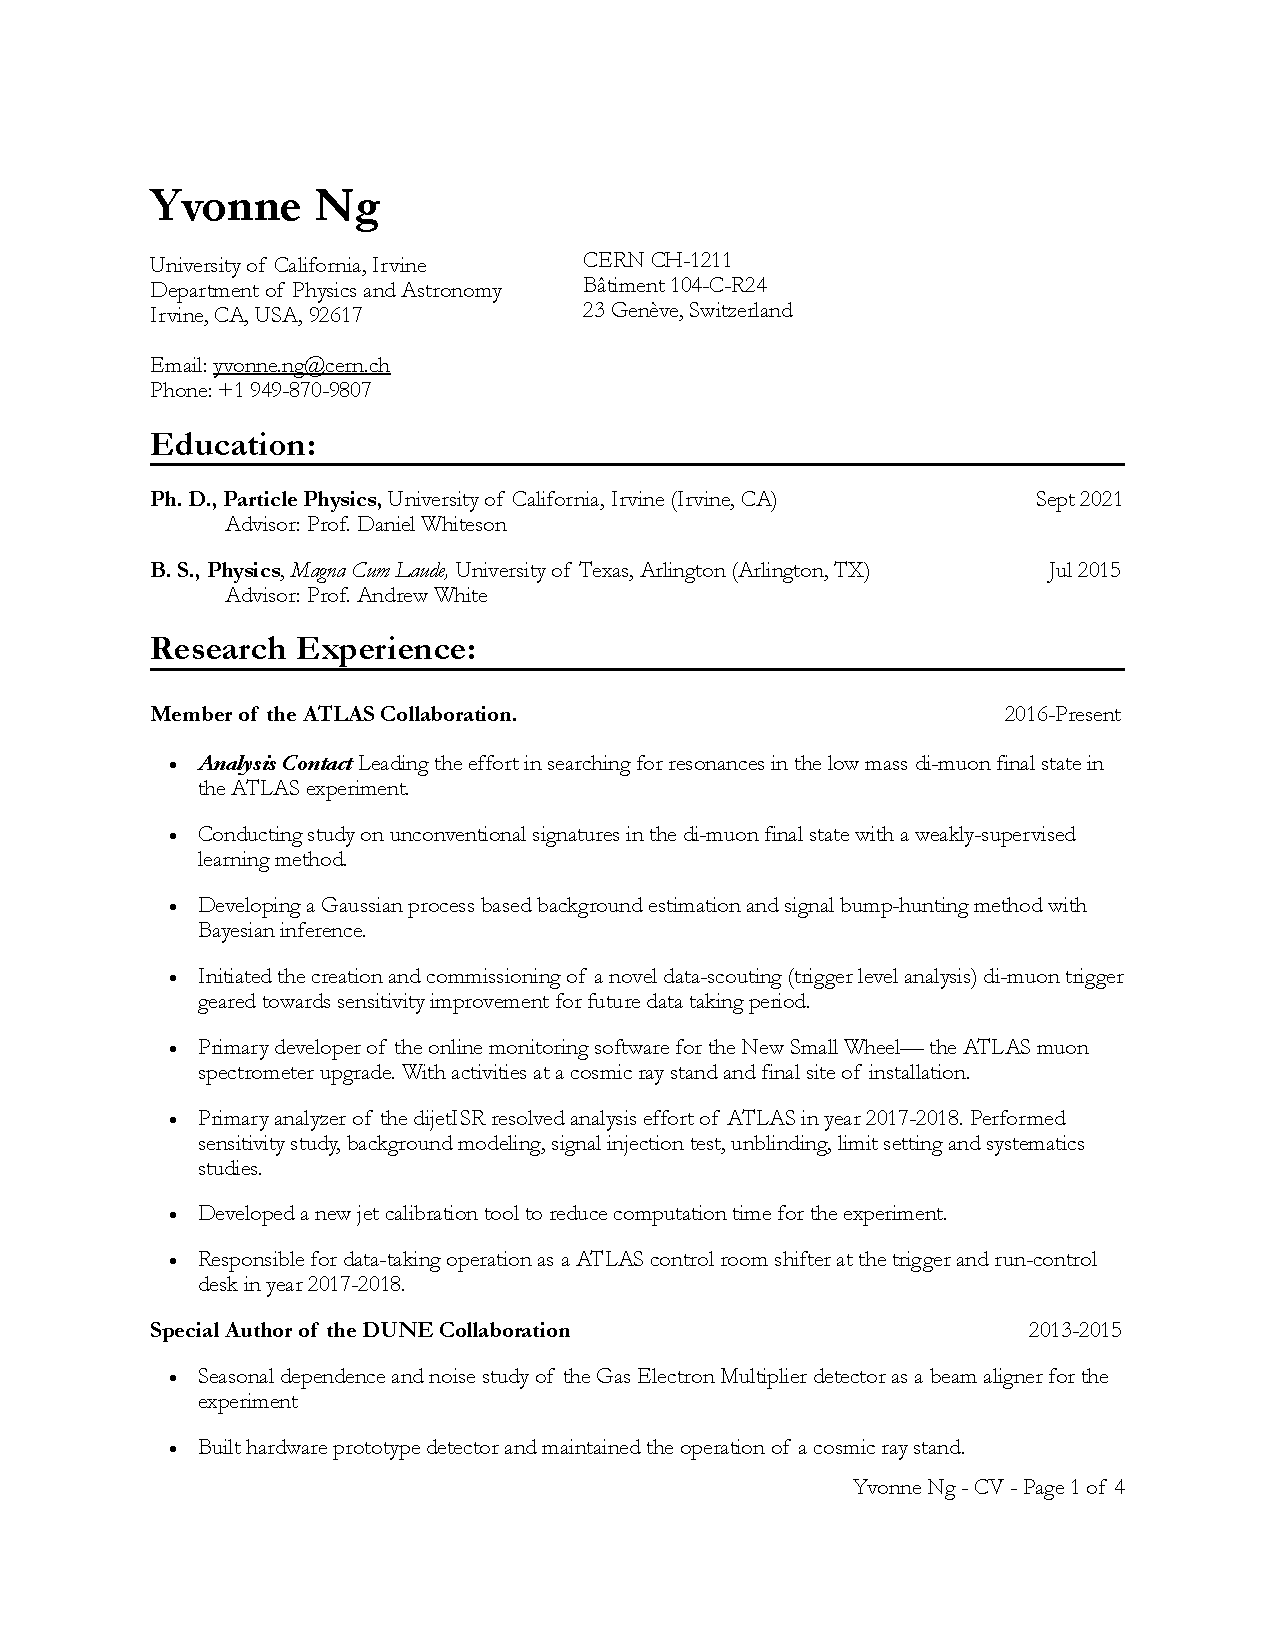
\includepdf[pages=-]{/Users/yvonne/WorkSpace/phd_thesis/phd_thesis/thesis/misc_metadata/cv/YWYvonneNg_CV_FermiLab.pdf}



%\textbf{EDUCATION}
%  
%  \begin{tabular*}{1\textwidth}{@{\extracolsep{\fill}}lr}
%    \textbf{Doctor of Philosophy in Computer Science} & \textbf{2012} \\
%    \vspace{6pt}
%    University name & \emph{City, State} \\
%    \textbf{Bachelor of Science in Computational Sciences} & \textbf{2007} \\
%    \vspace{6pt}
%    Another university name & \emph{City, State} \\
%  \end{tabular*}
%
%\vspace{12pt}
%\textbf{RESEARCH EXPERIENCE}
%
%  \begin{tabular*}{1\textwidth}{@{\extracolsep{\fill}}lr}
%    \textbf{Graduate Research Assistant} & \textbf{2007--2012} \\
%    \vspace{6pt}
%    University of California, Irvine & \emph{Irvine, California} \\
%  \end{tabular*}
%
%\vspace{12pt}
%\textbf{TEACHING EXPERIENCE}
%
%  \begin{tabular*}{1\textwidth}{@{\extracolsep{\fill}}lr}
%    \textbf{Teaching Assistant} & \textbf{2009--2010} \\
%    \vspace{6pt}
%    University name & \emph{City, State} \\
%  \end{tabular*}
%
%\pagebreak
%
%\textbf{REFEREED JOURNAL PUBLICATIONS}
%
%  \mypubentry{Ground-breaking article}{2012}{Journal name}
%
%\vspace{12pt}
%\textbf{REFEREED CONFERENCE PUBLICATIONS}
%
%  \mypubentry{Awesome paper}{Jun 2011}{Conference name}
%  \mypubentry{Another awesome paper}{Aug 2012}{Conference name}
%
%\vspace{12pt}
%\textbf{SOFTWARE}
%
%  \mysoftentry{Magical tool}{http://your.url.here/}
%  {C++ algorithm that solves TSP in polynomial time.}
%
}

% The abstract was previously limited to a maximum of 350 words, 
% but the UCI manual at https://etd.lib.uci.edu/electronic/td2e#2.2.1.
% currently does not indicate that there is any word limit for the abstract
\thesisabstract
{
  Many empirical evidence points to the existence of beyond-the-standard-model physics. In the LHC, different theoretical and experiemntal tehcniques are used to look for new particles as for new physics. One method with theoretical elegance and clean experimental reconstruction, is the resonance finding method. The method has enjoyed much sucesses in the past, W, Z and the Higgs boson are some of the few particles discovered this way. However, the early beyond-the-standard-model resonance search program of the LHC has returned empty handed. 
In this thesis, I ask the question of whether the standard approach could be modified to look for "weird resonances", particles that exist in the LHC dataset but goes beyond the standard program. Their discovery can provide important clue to beyond-the-standard-model physics. 

Three physics analyses beyond the usual search program are covered in this thesis. The first two on the dijetISR final state and the last one on dimuon final state. In the dijetISR searches, an ISR object is used to boost the final state. By triggering on the ISR object rather than the resonance formming final state, lower mass resonances can be covered. These two analysis set the lowest ATLAS low mass limit below the standard dijet search. In the dimuon search, as previous searches has neglected the low mass region below the Z peak, the search seeks to cover the region from 12-70 GeV. A novel statistical method driven by Gaussian Process is used. The method allow for a simple background estimation for a similar class of future analyses where Monte Carlo is limited.

All of these analyses provide competitive exclusion in the dark matter benchmark model of the LHC in places not previously covered.

As a future discussion, a new stream from trigger level analysis could be implemented to the dimuon search to improve the low mass sensitivity. Data driven approach like CWOLA can also be used to look for resonances free of an assumed signal model.

The thesis also covers involvement jet in-situ calibration as well as the new small wheel online monitoring software development.

"Weird resonances" are the "out-of-ordinary" ones: They are not a part of the current knowledge model; they break existing laws; they defies our knowledge about the world and human-beings; they are already somewhere out there, but only from its discovery it can be realized that we are more than what we think we are. The search for weird resonanances is a search for authenticity.

  %The abstract of your contribution goes here.
}


%%% Local Variables: ***
%%% mode: latex ***
%%% TeX-master: "thesis.tex" ***
%%% End: ***


% Add PDF document info fields
\hypersetup{
	pdftitle={\Thesistitle},
	pdfauthor={\Authorname},
	pdfsubject={\Degreefield},
}

% Uncomment the following to have numbered subsubsections (by default
% numbering goes only to subsections).
%\setcounter{secnumdepth}{4}


% Set this to only select a subset of the includes directives below.
% Very handy to speed up compilation if you're working on a certain
% part of your thesis. It conserves page numbers, references, etc.
% even for non-included files.

%% commands
\newcommand{\SUewk}{$\mathcal{SU}(2)_{L} \times \mathcal{U}(1)_{Y}$}
\newcommand*{\Uone}{$\mathcal{U}(1)$}
\newcommand{\SUtwo}{$\mathcal{SU}(2)$}
\newcommand{\SUthree}{$\mathcal{SU}(3)$}

\newcommand{\SML}{$\mathcal{L}_{\text{SM}}$}
\newcommand{\fieldQi}{$Q_i$}
\newcommand{\fieldUri}{$u_{\text{R},i}$}
\newcommand{\fieldDri}{$d_{\text{R},i}$}
\newcommand{\fieldLi}{$L_i$}
\newcommand{\fieldEri}{$e_{\text{R},i}$}
\newcommand{\fieldB}{$B$}
\newcommand{\fieldW}{$W$}
\newcommand{\fieldWone}{$W_1$}
\newcommand{\fieldWtwo}{$W_2$}
\newcommand{\fieldWthree}{$W_3$}
\newcommand{\fieldWp}{$W^+$}
\newcommand{\fieldWm}{$W^-$}
\newcommand{\fieldWzero}{$W^0$}
\newcommand{\fieldWpm}{$W^{\pm}$}
\newcommand{\fieldZ}{$Z$}
\newcommand{\fieldZzero}{$Z^0$}
\newcommand{\fieldPhoton}{$\gamma$}
\newcommand{\fieldG}{$G$}
\newcommand{\quarkU}{$u$}
\newcommand{\quarkD}{$d$}
\newcommand{\quarkC}{$c$}
\newcommand{\quarkS}{$s$}
\newcommand{\quarkT}{$t$}
\newcommand{\quarkB}{$b$}
\newcommand{\leptonE}{$e$}
\newcommand{\leptonMu}{$\mu$}
\newcommand{\leptonTau}{$\tau$}
\newcommand{\neutrinoE}{$\nu_e$}
\newcommand{\neutrinoMu}{$\nu_{\mu}$}
\newcommand{\neutrinoTau}{$\nu_{\tau}$}
\newcommand{\fieldUl}{$u_{\text{L}}$}
\newcommand{\fieldDl}{$d_{\text{L}}$}
\newcommand{\fieldCl}{$c_{\text{L}}$}
\newcommand{\fieldSl}{$s_{\text{L}}$}
\newcommand{\fieldTl}{$t_{\text{L}}$}
\newcommand{\fieldBl}{$b_{\text{L}}$}
\newcommand{\fieldUr}{$u_{\text{R}}$}
\newcommand{\fieldDr}{$d_{\text{R}}$}
\newcommand{\fieldCr}{$c_{\text{R}}$}
\newcommand{\fieldSr}{$s_{\text{R}}$}
\newcommand{\fieldTr}{$t_{\text{R}}$}
\newcommand{\fieldBr}{$b_{\text{R}}$}
\newcommand{\fieldEl}{$e_{\text{L}}$}
\newcommand{\fieldMul}{$\mu_{\text{L}}$}
\newcommand{\fieldTaul}{$\tau_{\text{L}}$}
\newcommand{\fieldEr}{$e_{\text{R}}$}
\newcommand{\fieldMur}{$\mu_{\text{R}}$}
\newcommand{\fieldTaur}{$\tau_{\text{R}}$}
\newcommand{\fieldNuEl}{$\nu_{e,\text{L}}$}
\newcommand{\fieldNuMul}{$\nu_{\mu,\text{L}}$}
\newcommand{\fieldNuTaul}{$\nu_{\tau,\text{L}}$}
\newcommand{\fieldNuR}{$\nu_{\text{R}}$}
\newcommand{\fieldPhi}{$\mathcal{\phi}$}
\newcommand{\fieldPhip}{$\mathcal{\phi}^+$}
\newcommand{\fieldPhizero}{$\mathcal{\phi}^0$}
\newcommand{\fieldH}{$h$}
\newcommand*{\TeV}{\ensuremath{\text{Te\kern -0.1em V}}}
\newcommand*{\GeV}{\ensuremath{\text{Ge\kern -0.1em V}}}
\newcommand*{\MeV}{\ensuremath{\text{Me\kern -0.1em V}}}
\newcommand*{\pT}{\ensuremath{p_{T}}}
\newcommand*{\micron}{\ensuremath{\mu m}}

\usepackage{xspace}
\newcommand*{\ptmiss}{\ensuremath{\mathbf{p}_{\text{T}}^{\text{miss}}}\xspace}
\newcommand*{\met}{\ensuremath{E_{\text{T}}^{\text{miss}}}\xspace}
\newcommand*{\antikt}{\ensuremath{\text{anti-}k_t}\xspace}
\newcommand*{\npv}{\ensuremath{N_{\text{PV}}}\xspace}

\newcommand*{\micromegas}{MicroMegas\xspace}
\newcommand*{\stgc}{sTGC\xspace}

\newcommand*{\ttbar}{\ensuremath{t\bar{t}}}
\newcommand*{\wt}{\ensuremath{Wt}}
\newcommand*{\zhf}{$Z$+HF}
\newcommand*{\vv}{\ensuremath{VV}}
\newcommand*{\cls}{\ensuremath{\text{CL}_{\text{s}}}\xspace}

% BSM

\newcommand*{\nino}{\ensuremath{\mathchoice%
      {\displaystyle\raise.4ex\hbox{$\displaystyle\tilde\chi^0$}}%
         {\textstyle\raise.4ex\hbox{$\textstyle\tilde\chi^0$}}%
       {\scriptstyle\raise.3ex\hbox{$\scriptstyle\tilde\chi^0$}}%
 {\scriptscriptstyle\raise.3ex\hbox{$\scriptscriptstyle\tilde\chi^0$}}}\xspace}
\newcommand*{\ninoone}{\ensuremath{\mathchoice%
      {\displaystyle\raise.4ex\hbox{$\displaystyle\tilde\chi^0_1$}}%
         {\textstyle\raise.4ex\hbox{$\textstyle\tilde\chi^0_1$}}%
       {\scriptstyle\raise.3ex\hbox{$\scriptstyle\tilde\chi^0_1$}}%
 {\scriptscriptstyle\raise.3ex\hbox{$\scriptscriptstyle\tilde\chi^0_1$}}}\xspace}
\newcommand*{\ninotwo}{\ensuremath{\mathchoice%
      {\displaystyle\raise.4ex\hbox{$\displaystyle\tilde\chi^0_2$}}%
         {\textstyle\raise.4ex\hbox{$\textstyle\tilde\chi^0_2$}}%
       {\scriptstyle\raise.3ex\hbox{$\scriptstyle\tilde\chi^0_2$}}%
 {\scriptscriptstyle\raise.3ex\hbox{$\scriptscriptstyle\tilde\chi^0_2$}}}\xspace}
\newcommand*{\ninothree}{\ensuremath{\mathchoice%
      {\displaystyle\raise.4ex\hbox{$\displaystyle\tilde\chi^0_3$}}%
         {\textstyle\raise.4ex\hbox{$\textstyle\tilde\chi^0_3$}}%
       {\scriptstyle\raise.3ex\hbox{$\scriptstyle\tilde\chi^0_3$}}%
 {\scriptscriptstyle\raise.3ex\hbox{$\scriptscriptstyle\tilde\chi^0_3$}}}\xspace}
\newcommand*{\ninofour}{\ensuremath{\mathchoice%
      {\displaystyle\raise.4ex\hbox{$\displaystyle\tilde\chi^0_4$}}%
         {\textstyle\raise.4ex\hbox{$\textstyle\tilde\chi^0_4$}}%
       {\scriptstyle\raise.3ex\hbox{$\scriptstyle\tilde\chi^0_4$}}%
 {\scriptscriptstyle\raise.3ex\hbox{$\scriptscriptstyle\tilde\chi^0_4$}}}\xspace}
\newcommand*{\chinoonep}{\ensuremath{\mathchoice%
      {\displaystyle\raise.4ex\hbox{$\displaystyle\tilde\chi^+_1$}}%
         {\textstyle\raise.4ex\hbox{$\textstyle\tilde\chi^+_1$}}%
       {\scriptstyle\raise.3ex\hbox{$\scriptstyle\tilde\chi^+_1$}}%
 {\scriptscriptstyle\raise.3ex\hbox{$\scriptscriptstyle\tilde\chi^+_1$}}}\xspace}
\newcommand*{\chinoonem}{\ensuremath{\mathchoice%
      {\displaystyle\raise.4ex\hbox{$\displaystyle\tilde\chi^-_1$}}%
         {\textstyle\raise.4ex\hbox{$\textstyle\tilde\chi^-_1$}}%
       {\scriptstyle\raise.3ex\hbox{$\scriptstyle\tilde\chi^-_1$}}%
 {\scriptscriptstyle\raise.3ex\hbox{$\scriptscriptstyle\tilde\chi^-_1$}}}\xspace}
\newcommand*{\chinoonepm}{\ensuremath{\mathchoice%
      {\displaystyle\raise.4ex\hbox{$\displaystyle\tilde\chi^\pm_1$}}%
         {\textstyle\raise.4ex\hbox{$\textstyle\tilde\chi^\pm_1$}}%
       {\scriptstyle\raise.3ex\hbox{$\scriptstyle\tilde\chi^\pm_1$}}%
 {\scriptscriptstyle\raise.3ex\hbox{$\scriptscriptstyle\tilde\chi^\pm_1$}}}\xspace}

\newcommand*{\chinotwop}{\ensuremath{\mathchoice%
      {\displaystyle\raise.4ex\hbox{$\displaystyle\tilde\chi^+_2$}}%
         {\textstyle\raise.4ex\hbox{$\textstyle\tilde\chi^+_2$}}%
       {\scriptstyle\raise.3ex\hbox{$\scriptstyle\tilde\chi^+_2$}}%
 {\scriptscriptstyle\raise.3ex\hbox{$\scriptscriptstyle\tilde\chi^+_2$}}}\xspace}
\newcommand*{\chinotwom}{\ensuremath{\mathchoice%
      {\displaystyle\raise.4ex\hbox{$\displaystyle\tilde\chi^-_2$}}%
         {\textstyle\raise.4ex\hbox{$\textstyle\tilde\chi^-_2$}}%
       {\scriptstyle\raise.3ex\hbox{$\scriptstyle\tilde\chi^-_2$}}%
 {\scriptscriptstyle\raise.3ex\hbox{$\scriptscriptstyle\tilde\chi^-_2$}}}\xspace}
\newcommand*{\chinotwopm}{\ensuremath{\mathchoice%
      {\displaystyle\raise.4ex\hbox{$\displaystyle\tilde\chi^\pm_2$}}%
         {\textstyle\raise.4ex\hbox{$\textstyle\tilde\chi^\pm_2$}}%
       {\scriptstyle\raise.3ex\hbox{$\scriptstyle\tilde\chi^\pm_2$}}%
 {\scriptscriptstyle\raise.3ex\hbox{$\scriptscriptstyle\tilde\chi^\pm_2$}}}\xspace}
\newcommand*{\chinop}{\ensuremath{\mathchoice%
      {\displaystyle\raise.4ex\hbox{$\displaystyle\tilde\chi^+$}}%
         {\textstyle\raise.4ex\hbox{$\textstyle\tilde\chi^+$}}%
       {\scriptstyle\raise.3ex\hbox{$\scriptstyle\tilde\chi^+$}}%
 {\scriptscriptstyle\raise.3ex\hbox{$\scriptscriptstyle\tilde\chi^+$}}}\xspace}
\newcommand*{\chinom}{\ensuremath{\mathchoice%
      {\displaystyle\raise.4ex\hbox{$\displaystyle\tilde\chi^-$}}%
         {\textstyle\raise.4ex\hbox{$\textstyle\tilde\chi^-$}}%
       {\scriptstyle\raise.3ex\hbox{$\scriptstyle\tilde\chi^-$}}%
 {\scriptscriptstyle\raise.3ex\hbox{$\scriptscriptstyle\tilde\chi^-$}}}\xspace}
\newcommand*{\chinopm}{\ensuremath{\mathchoice%
      {\displaystyle\raise.4ex\hbox{$\displaystyle\tilde\chi^\pm$}}%
         {\textstyle\raise.4ex\hbox{$\textstyle\tilde\chi^\pm$}}%
       {\scriptstyle\raise.3ex\hbox{$\scriptstyle\tilde\chi^\pm$}}%
 {\scriptscriptstyle\raise.3ex\hbox{$\scriptscriptstyle\tilde\chi^\pm$}}}\xspace}
\newcommand*{\chinomp}{\ensuremath{\mathchoice%
      {\displaystyle\raise.4ex\hbox{$\displaystyle\tilde\chi^\mp$}}%
         {\textstyle\raise.4ex\hbox{$\textstyle\tilde\chi^\mp$}}%
       {\scriptstyle\raise.3ex\hbox{$\scriptstyle\tilde\chi^\mp$}}%
 {\scriptscriptstyle\raise.3ex\hbox{$\scriptscriptstyle\tilde\chi^\mp$}}}\xspace}
\newcommand*{\squark}{\ensuremath{\tilde{q}}\xspace}
\newcommand*{\squarkL}{\ensuremath{\tilde{q}_{\mathrm{L}}}\xspace}
\newcommand*{\squarkR}{\ensuremath{\tilde{q}_{\mathrm{R}}}\xspace}
\newcommand*{\gluino}{\ensuremath{\tilde{g}}\xspace}
\renewcommand*{\stop}{\ensuremath{\tilde{t}}\xspace}
\newcommand*{\stopone}{\ensuremath{\tilde{t}_1}\xspace}
\newcommand*{\stoptwo}{\ensuremath{\tilde{t}_2}\xspace}
\newcommand*{\stopL}{\ensuremath{\tilde{t}_{\mathrm{L}}}\xspace}
\newcommand*{\stopR}{\ensuremath{\tilde{t}_{\mathrm{R}}}\xspace}
\newcommand*{\sbottom}{\ensuremath{\tilde{b}}\xspace}
\newcommand*{\sbottomone}{\ensuremath{\tilde{b}_1}\xspace}
\newcommand*{\sbottomtwo}{\ensuremath{\tilde{b}_2}\xspace}
\newcommand*{\sbottomL}{\ensuremath{\tilde{b}_{\mathrm{L}}}\xspace}
\newcommand*{\sbottomR}{\ensuremath{\tilde{b}_{\mathrm{R}}}\xspace}
\newcommand*{\slepton}{\ensuremath{\tilde{\ell}}\xspace}
\newcommand*{\sleptonL}{\ensuremath{\tilde{\ell}_{\mathrm{L}}}\xspace}
\newcommand*{\sleptonR}{\ensuremath{\tilde{\ell}_{\mathrm{R}}}\xspace}
\newcommand*{\sel}{\ensuremath{\tilde{e}}\xspace}
\newcommand*{\selL}{\ensuremath{\tilde{e}_{\mathrm{L}}}\xspace}
\newcommand*{\selR}{\ensuremath{\tilde{e}_{\mathrm{R}}}\xspace}
\newcommand*{\smu}{\ensuremath{\tilde{\mu}}\xspace}
\newcommand*{\smuL}{\ensuremath{\tilde{\mu}_{\mathrm{L}}}\xspace}
\newcommand*{\smuR}{\ensuremath{\tilde{\mu}_{\mathrm{R}}}\xspace}
\newcommand*{\stau}{\ensuremath{\tilde{\tau}}\xspace}
\newcommand*{\stauL}{\ensuremath{\tilde{\tau}_{\mathrm{L}}}\xspace}
\newcommand*{\stauR}{\ensuremath{\tilde{\tau}_{\mathrm{R}}}\xspace}
\newcommand*{\stauone}{\ensuremath{\tilde{\tau}_1}\xspace}
\newcommand*{\stautwo}{\ensuremath{\tilde{\tau}_2}\xspace}
\newcommand*{\snu}{\ensuremath{\tilde{\nu}}\xspace}
\newcommand*{\sdiff}{\ensuremath{\Delta m (\stopone, \ninoone)}\xspace}

% RJR VAR
\newcommand*{\dpb}{\ensuremath{\Delta \phi (\vec{\beta}_{PP}^{\,\text{LAB}}, \vec{p}_V^{\,PP})}\xspace}
\newcommand*{\mdr}{\ensuremath{E_V^P}\xspace}
\newcommand*{\gaminv}{\ensuremath{1/\gamma_P^{PP}}\xspace}
\newcommand*{\cosb}{\ensuremath{\cos\theta_b}\xspace}
\newcommand*{\rpt}{\ensuremath{R_{p_T}}\xspace}
\newcommand*{\bWN}{\ensuremath{\stopone\rightarrow b W \ninoone}\xspace}
\newcommand*{\msn}{\ensuremath{(m_{\stopone}, m_{\ninoone})}\xspace}

% HH
\newcommand*{\sigmaUL}{\ensuremath{\sigma^{\text{UL}}}\xspace}
\newcommand*{\sigmaSM}{\ensuremath{\sigma^{\text{SM}}}\xspace}
\newcommand*{\sigmaHH}{\ensuremath{\sigma_{hh}}\xspace}
\newcommand*{\sigmaHHSM}{\ensuremath{\sigma_{hh}^{\text{SM}}}\xspace}
\newcommand*{\sigmaHHUL}{\ensuremath{\sigma_{hh}^{\text{UL}}}\xspace}
\newcommand*{\sigmaRatio}{\ensuremath{\sigmaUL / \sigmaSM}\xspace}
\newcommand*{\bbbb}{\ensuremath{4b}\xspace}
\newcommand*{\bbtautau}{\ensuremath{bb\tau\tau}\xspace}
\newcommand*{\bbyy}{\ensuremath{bb\gamma\gamma}\xspace}
\newcommand*{\bbll}{\ensuremath{bb\ell\ell}\xspace}
\newcommand*{\bbww}{\ensuremath{bbWW^*}\xspace}
\newcommand*{\bbllX}{\ensreumath{bbWW^*+bbZZ^*+bb\tau\tau}\xspace}
\newcommand*{\wwww}{\ensuremath{4W}\xspace}
\newcommand*{\wwyy}{\ensuremath{WW^*\gamma\gamma}\xspace}
\newcommand*{\bbwwtwo}{\ensuremath{\bbww,2\ell}\xspace}

\newcommand*{\mll}{\ensuremath{m_{\ell\ell}}\xspace}
\newcommand*{\ptll}{\ensuremath{p_{\text{T}}^{\ell\ell}}\xspace}
\newcommand*{\dphimetll}{\ensuremath{\Delta \phi (\bm{p}_{\text{T}}^{\text{miss}}, \bm{p}_{\text{T}}^{\ell\ell})}\xspace}
\newcommand*{\metll}{\ensuremath{\bm{p}_{\text{T}}^{\text{miss}} + \bm{p}_{\text{T}}^{\ell \ell}}\xspace}
\newcommand*{\dphibb}{\ensuremath{\Delta \phi_{bb}}\xspace}
\newcommand*{\httwo}{\ensuremath{H_{\text{T2}}}\xspace}
\newcommand*{\htratio}{\ensuremath{H_{\text{T2}}^{R}}\xspace}
\newcommand*{\mttwo}{\ensuremath{m_{\text{T2}}}\xspace}
\newcommand*{\mtbb}{\ensuremath{m_{\text{T2}}^{bb}}\xspace}
\newcommand*{\drll}{\ensuremath{\Delta R_{\ell\ell}}\xspace}
\newcommand*{\drbb}{\ensuremath{\Delta R_{bb}}\xspace}
\newcommand*{\dphill}{\ensuremath{\Delta \phi_{\ell\ell}}\xspace}
\newcommand*{\phh}{\ensuremath{ p_{hh}}\xspace}
\newcommand*{\ptop}{\ensuremath{ p_{\text{Top}}}\xspace}
\newcommand*{\pzsf}{\ensuremath{ p_{Z-\text{SF}}}\xspace}
\newcommand*{\pztt}{\ensuremath{ p_{Z-\tau\tau}}\xspace}
\newcommand*{\dhh}{\ensuremath{ d_{hh}}\xspace}
\newcommand*{\dtop}{\ensuremath{ d_{\text{Top}}}\xspace}
\newcommand*{\dzsf}{\ensuremath{ d_{Z-\text{SF}}}\xspace}
\newcommand*{\dztt}{\ensuremath{ d_{Z-\tau\tau}}\xspace}

\newcommand*{\htnum}{\ensuremath{|\bm{p}_{\text{T}}^{\text{miss}} + \bm{p}_{\text{T}}^{\ell,0} + \bm{p}_{\text{T}}^{\ell,1}| + | \bm{p}_{\text{T}}^{b,0} + \bm{p}_{\text{T}}^{b,1}|}\xspace}
\newcommand*{\htden}{\ensuremath{|\bm{p}_{\text{T}}^{\text{miss}}| + |\bm{p}_{\text{T}}^{\ell,0}| + |\bm{p}_{\text{T}}^{\ell,1}| + |\bm{p}_{\text{T}}^{b,0}| + |\bm{p}_{\text{T}}^{b,1}|}\xspace}
\newcommand{\ptvec}[2]{\ensuremath{\mathbf{p}_{\text{T}}^{#1#2}}\xspace}

\DeclareMathAlphabet\mathbfcal{OMS}{cmsy}{b}{n}

\begin{document}
% Preliminary pages are always loaded (TOC, CV, etc.})
\preliminarypages

% if doing minimal compilation just add the table of contents here, otherwise use the "\preliminarypages" command above
%\tableofcontents

% set the linespacing for the internal text
\onehalfspacing

% Include the different components of your thesis, in separate files.
% Using \include allows you to set \includeonly above.
%\include{chapter1}
%\include{chapter2}
% ... and so on

% start START
\setcounter{page}{0}

\chapter{Introduction}

% Searching for truth is part of what makes us human. 
An eagerness for the truth is part of what makes us human. This has been true across cultures through different times: ancient Greeks who toyed with mathematics of trigonometric objects saw an eternal truth in their beauty; in the Eastern Zhou Dynasty of China\footnote{Eastern Zhou is a Chinese dynasty that existed between 771 to 476 BCE. Influential scholars include \textit{Confucious}, \textit{Lao-tse}, and \textit{Mo-tse}.}, influential scholars debated the truthful nature of humans and,
therefore, their subsequent duty; driven by the same thirst, in modern days humans took to space, went on the moon and began exploring the extra-terrestrial frontier for beyond earth. The aspiration for truth formed knowledge. It has advanced technology, medicine, law, science, and human psychology. \textit{Everything} in our civilization derives from this ambition in humans to seek truth.

%advance different technology, allow human to live for longer with greater convenience and provide a deeper understanding on the human nature. 
%different streams of Indian philosophers debates and discuss the Satya (loosly translate to truth) and its practice.
%distinction between the world of phenomenon and nomenon, the latter describe a part of world that is beyond our senses but describe the fundamental nature of things. 

Human's endeavor for the truth is always to uncover something more than what is already known: over two thousand years ago, Plato saw the truth in the \textit{ideal forms} beyond the shadow projections of everyday things~\cite{plato1961republic}; Amongst the mechanical industrial world view 19th century, Immanuel Kant postulated a world of the \textit{transcendental},  a world of the fundamental
nature of things, behind the world of \textit{phenomena}, of human senses~\cite{kant1908critique}.\footnote{Kant in his famous book the Critque of Pure Reasons~\cite{kant1908critique} call this world of the transcedentals the \textit{noumenon} (contrasting with the world
of \textit{phenomenon} that can be perceived by human senses.
Kant believes this \textit{transcendental} realm that we have no access to is actually the true nature of things. The \textit{transcendental} is sometime referred to as the \textit{thing-in-itself}.)}. In contemporary times of the $21^{st}$ century, faced with the clash of cultures and perspectives facilitated by the internet and modern transportation, truth is no longer seen as a static set of doctrine or statements of facts in the older days\footnote{The view of truth as a
direct correspondence to facts is known as the Correspondence theory
of truth~\cite{sep-truth-correspondence}. Detail objections to the theory can be found in the reference.}, but humans' endeavor to the truth has not stopped.

Combined with the idea of subjectivity, contemporary philosopher Alain Badiou has formulated the logic for the search for truth as "truth procedures": truth is the subsequent discourses and knowledge re-development that follows from a rupture or an accident\footnote{Badiou called such rupture or accident an \textit{Event}} that shatters our existing knowledge system~\cite{badiou2007being}. This "truth procedure" echoes ideas from Thomas Kuhn on scientific \textit{paradigm
shifts}~\cite{kuhn2021structure}, but also describes truth seeking as part of individual \textit{ethics}. "There is always only one question in the ethics of truth", Badiou wrote, "how will I, as someone, continue to exceed my own being?"\cite{badiou2002ethics}. The search for truth is not seen merely a human desire, but also a moral duty to remain authentic to himself/herself.

%The ingrained search of truth in human nature shows a fundamental quest to authenticity, and that human can be more than what we believe we are. 
% philosophy no longer treat truth as an ideal like Plato, or mechanical statics like in the early 20th century, but it's nonetheless a human drive to

Particle physics is a search for truth in the most elementary form. It seeks to understand fundamental particles and their interaction as building blocks to the world around. Not only does it expands knowledge of the smallest possible observable universe, but it is also a study of the things that constitute chemicals, biological cells, animals, highrise structures, and \textit{everything else} under the physical realm. Knowledge in particle physics is also tightly related to objects of the largest scale, namely cosmology, knowledge in particle physics affects the structure of the entire universe, its evolution and is essential to answering questions on the origin of the human.

Particle Physics as a field was developed in the 1960s together with advances in Quantum Field Theory. Through new experimental findings and new theoretical model-building techniques, the Standard Model of Particle Physics was established. The theory is the epitome of human's understanding on the fundamental building block of the universe. The model enjoyed many successes: many predictions made were later confirmed by experimental findings. The $J/\Psi$, $Z$, and the Higgs Boson are all discovered that way. Human
understanding of matter, its origin, and the governing laws between the interactions has since been greatly advanced. 

However, even with its success, there remain many open questions to the Standard Model of Particle Physics. %Or in Badiou's term, many "accidents" have ruptured the current understanding of particle physics, a truth procedure is in need repaired the tear in understanding.
For example, the Standard Model in its current form does not describe gravity or any of its interactions; there is a mathematically unnatural fine tuning of several parameters in the theory; in addition, the
Standard Model also does not include dark matter, which makes up the majority of the matter (~85\% ) of the universe or dark energy, which in 
Einstein's theory explained the expanding universe seen today.  

One way of fixing the inconsistency is by finding new particles predicted by different theoretical hypotheses. One way to find these new particles  is through high-energy particle collisions. If dark matter interacted weakly with Standard Model particles in the early universe like many theoretical models have come to predict, it would be possible for them to be produced through high-energy collisions of Standard Model particles. One possible signature of Dark matter can be searched in forms of Dark Matter mediator that appears as anomalous resonances.

This thesis offers a few humble attempts to resolve some of these standing problems in the Standard Model of particle physics by discovering new particles that would offer extra insights to future theory building. These are done by attempting to create previously unobserved conditions in high-energy particle collisions via the Large Hadron Collider. It uses data collected by the ATLAS experiment in the Large Hadron Collider. These new particles, if discovered, as little inconsistencies to the Standard Model of Particle
Physics, are nuggets to truth. It has great potential to add to our understanding of fundamental particle physics.

The thesis is organized as the following: chapter~\ref{chapter:SM} describes the history and the description of the Standard Model; chapter ~\ref{chapter:DM} discusses the theory of dark matter; chapter~\ref{chapter:ATLAS} presents the experimental setup of the Large Hadron Collider and the ATLAS experiment;
chapter~\ref{chapter:common_analysis_items} covers the common analysis items (reconstruction
of objects )and their preparation before the analyses; Chapter~\ref{chapter:dijetISR}-~\ref{chapter:dimuon} outline the analyses that I played a major part in, namely the dijet resolved analysis, and the low mass dimuon analysis; this thesis also covers a future direction for resonance finding in collider physics in Chapter~\ref{chapter:topo}, that discusses uncovered resonances in the two body final states. These novel techniques, together with theory-driven approaches, could hold keys to unlocking the next finding that can revolutionalize our current understanding of particle physics. 

The pursuit of \textit{Aletheia}(truth) is a nessessity to human \textit{authenticity}, as philosopher Martin Heideigger famously put. This thesis could be seen as a humble response in face of such human condition, or a fulfillment of an ethical duty to remain \textit{authentic}, even if nothing more was achieved. But perhaps there is still more to the pursuit than any eloquent philosopher can ever formulate: it is an adventure of
joy and pleasure to uncovering all things unknown. It is a journey that reminds us, what we are is always more than what we know.

%To summarize the section with a a reason that drives this attempt and many other that would follow: what's in the \textit{real} behind the surface, is always worth uncovering, not only as a ethical duty as stated by many philospher, but this is also a pursue done out of a sense of joy and pleasure in truth finding: we are always more than what we _know_ we are.

%Truth(\textit{Aletheia}) is not mere correspondence to facts, but rather a human(\textit{Dasein})-involving process to to _unconceal_ what is in the real.

%The search of truth is the uncovering of facade in front for authenticity and admitting of our ignorance, there is something more than what we currently know to be uncovered:  
% As Martin Heidigger would put it. 

%Plato in his allegory of the cave illustrates truth as ideal forms behind the shadows that human sees.
%The search of truth is an act of authenticity

%Truth is no longer viewed as a static, but still something that human strive to get close to in our different endeavour in the realm of particle. In search for the strange little resonances, ooking for such rupture in the truth fabric, 

%Searching for truth is the search for that there is more than what is before us. 



%- Cannot know to what we can know
%Extending the frontier to what human know 

%Particle physics is the study of the most fundamental particles in the universe and their interaction. It's at the boundary of what it's known

%This thesis focuses on a series of searches done over resonance hunting 
%they are well motivated initially on the dark matter model, which is detailed in chapter . 

%Chapter discuss and review resonance hunting over smooth background, and give a discussion on how it is possible to look for new particle in dark matter model and beyond with this method.
%Literature on this will be further discussed and some pilot studies on the different methods of looking for new particle is reviewed here. Some inital dimuon results is shown. 

%Search for truth and something more is something fundamental and 

%The signature itself and i

%2. 

%An introduction to why what we are is more than, the overview of standard model strive to give an account for the history of the standard model of particle physics, 
%In search of truth, theory is perfected in the process, and that it is in this process that we gain tools to look for further truth.
%It's possible for human to be more than what we know. We are more than what we are. 

%* Psychoanalysis 
%Lacan in lack in jouissance. 
%The only unexplored region is the science of jouissance, the science of pleasure. 

%* Other unexpected signatures of particle physics not driven by models, the unexplored landscape of two body resonances. 




\chapter{The Standard Model of Particle Physics}
\label{chapter:SM}

%\epigraph{\textit{So it goes...}}{---Kurt Vonnegut, \textit{Slaughterhouse
%		Five}}
	
\epigraph{\textit{Ex pede Herculem. \newline(From the feet, Hercules.)}}{--Herodotus, Book IV, Section LXXXII. Plutarch.}

%A deep understanding of something small in great details gives you understanding of everything else. 

%\epigraph{\textit{Quote}}{--Unknown, \textit{}}
%\epigraph{\textit{Quote}}{--Person}


\section{Description}
The Standard Model of Particle Physics is the epitome of human's understanding to elementary building blocks of the physical world and to-date. It lays out seventeen particles, their propeties and interaction, in the three fundamental forces, the electromagnetic, the weak and the strong force. Everyday movements, from fliping the page of a book, to transportation; from weak beta decay in atomic decay to interaction of quarks within an atom nucluei, can be described by Stanard Model
particles and their interactions.

The Standard Model of Particle Physics is a gauge theory under the quantum field theory framework. Particles are represented different quantized fields operators. The particles interactions are determined by the standard model Lagrangian. Like other physic theories, the Lagrangian of the Standard Model observes physics symmetries.

\subsection*{Symmetry}
    Symmetry is the foundation to many laws in physics including the standard model. The Noether's Theorem has elegantly linked different symmetries to different conserved quantity: 

    %\begin{description}[font=$\bullet$~\normalfont\scshape\color{black!50!black}]
    \begin{itemize}
        \item Spatial Translational Symmetry $\rightarrow$ Translational Momentum Conservation

        \item Time Symmetry $\rightarrow$ Energy Conservation

        \item Rotational Symmetry $\rightarrow$ Angular Momentum Conservation

    \end{itemize}

Following from the Special Relativitiy, the invariance is applicable to all observers in different frames, and the above three can be summarized by the Lorentz symmetry ($\mathcal{P}$) and a transformation in the Lorentz group. The invariance quantity under this transformation is called the Lorentz invariance. 
    Apart from the Lorentz invariance, the Standard Model also observes internal local symmetries between particles. Namely  \SUthree$_C \times $ \SUtwo$_L \times$\Uone$_{Y}$, these internal symmetries describes the particle interactions and as "transformations" between different particles, oweing to the property of a gauge theory, these transformation are mediated by mediator particles. The different physical invariant quantities that are conserved under these particle
    transformation/interactions are called "charges", their interactions processes are sometimes called "currents".

    The influence of the individual part of the internal symmetries are described as follows: The local $SU(3)_{C}$ symmetry govern the strong force and only has an effect on particles with a color charge (either red, green or blue). These particles in the Standard Model include quarks of field $\mathcal{Q}_{i}$, which include the left handed doublets of (uL, dL), (cL, sL), (tL, bL). The symmetry also affect quark fields of right-handed singlets of $\mathcal{u}_R,i$ and $\mathcal{d}_R$. The
    strong force is mediated by the eight gluon fields $\mathcal{G}$.

    The $SU(2)_{L}$ transformation describes the weak force and is effective on particles with the weak charge, it is mediated by three W bosons (W1,W2,W3), the $U(1)$ transformation is meditated by the weak boson B and acts on particles that has a weak hyper-charge Y. The combined effect of the of the weak field and the weak hyper-charge field give us the familiar electro-magnetic weak force in day-to-day (including the LHC) energy scale below the spontaneous symmetry breaking, and has an
effect on most quark fields, bosons, as well as leptonic fields, which include the lepton field of left handed doublets of ($e_{L}$, $\nu_{e,L}$), ($\mu_{L}$, $\nu_{\mu,L}$), ($\tau_{L}$, $\nu_{\tau,L}$) and the right-handed singlets of $e_{R}$, $\mu_{R}$ and $\tau_{R}$.
    
    %The combined effect of the $SU(2)_L \times U(1)_{Y}$ gives us the familiar effect of electromagnetism/weak force effect below the spontaneous symmetry breaking scale, and affect the Q field described above, as well as the leptonic field of \mathcal{L}$_{i}$ 

\begin{table}[!htb]
    \begin{center}
        \begin{tabularx}{0.8\textwidth}{m{1em} c c c c c c c }
        \toprule
        \hline
& Field & Members & Spin & \Uone$_{Y}$) & \SUtwo$_{L}$ & \SUthree$_{C}$ \\
        \hline

        %\rotatebox{90}{\hspace{-0.1cm}\textbf{Fermionic Field} }
            \rotatebox{90}{\hspace{-0.1cm}\textbf{Leptons} }
             &   \makecell{\fieldLi \\ \fieldEri} % FIELD
             &   \makecell{ (\fieldEl, \fieldNuEl), (\fieldMul, \fieldNuMul), (\fieldTaul, \fieldNuTaul) \\ \fieldEr, \fieldMur, \fieldTaur}% CONTENT
             &   \makecell{ $1/2$ \\ $1/2$ }% SPIN
             &   \makecell{ $-1$ \\ $-2$ }% U(1)
             &   \makecell{ $\mathbf{2}$ \\ $\mathbf{1}$ }% SU(2)
             &   \makecell{ $\mathbf{1}$ \\ $\mathbf{1}$ } \\ % SU(3)
            \midrule
            \rotatebox{90}{\hspace{-0.1cm}\textbf{Quarks} } 
             &   \makecell{\fieldQi \\ \fieldUri \\ \fieldDri} % FIELD
             &   \makecell{ (\fieldUl, \fieldDl), (\fieldCl, \fieldSl), (\fieldTl, \fieldBl) \\ \fieldUr \\ \fieldDr}% CONTENT
             &   \makecell{ $1/2$ \\ $1/2$ \\ $1/2$} % SPIN
             &   \makecell{ $1/3$ \\ $4/3$ \\ $-2/3$}% U(1)
             &   \makecell{ $\mathbf{2}$ \\ $\mathbf{1}$ \\ $\mathbf{1}$}% SU(2)
             &   \makecell{ $\mathbf{3}$ \\ $\mathbf{3}$ \\ $\mathbf{3}$}\\ % SU(3)

        \cdashline{1-7}

        %\rotatebox{90}{\hspace{-0.1cm}\textbf{Bosonic Field} }
            \rotatebox{90}{\textbf{\stackanchor{Gauge}{Fields}} }
             &   \makecell{\fieldB \\ \fieldW \\ \fieldG } % FIELD
             &   \makecell{ \fieldB \\ (\fieldWone, \fieldWtwo, \fieldWthree) \\ \fieldG$_a$, $a\in[1,..,8]$ }% CONTENT
             &   \makecell{ $1$ \\ $1$ \\ $1$} % SPIN
             &   \makecell{ $0$ \\ $0$ \\ $0$}% U(1)
             &   \makecell{ $\mathbf{1}$ \\ $\mathbf{3}$ \\ $\mathbf{1}$}% SU(2)
             &   \makecell{ $\mathbf{1}$ \\ $\mathbf{1}$ \\ $\mathbf{8}$}\\ % SU(3)
            \midrule
            \rotatebox{90}{\textbf{\stackanchor{Higgs}{Field}}} 
             &   \makecell{\fieldPhi } % FIELD
             &   \makecell{ (\fieldPhip, \fieldPhizero) }% CONTENT
             &   \makecell{ $0$  } % SPIN
             &   \makecell{ $1$  }% U(1)
             &   \makecell{ $\mathbf{2}$ }% SU(2)
             &   \makecell{ $\mathbf{1}$ }\\ % SU(3)
        \hline
        \bottomrule
        \end{tabularx}
    \end{center}

    \caption{
        The particle fields of the SM\cite{Antrim:2699575}.
    \label{table:sm1}
    }

\end{table}

\FloatBarrier


A detailed list of the gauge fields field and their charges along with their mathematical group can be found in table~\ref{table:sm}~\cite{Antrim:2699575}. 

\subsection*{Spontaneous Symmetry Breaking}
The standard model theory in the form as presented in the last section does not give mass to the particles, this is inconsistent with observation in experiment, hyper The process of giving mass to the particle process is called the spontaneous symmetry breaking process.
[More details later]
%A scalar field with the name of the Higgs field, is coupled to the \SUtwo$_L$ \times \Uone$_Y$ group weak-hyper charge. The potential of the field has the shape of a Mexican hat, 


\begin{table}[!htb]
    \caption{
        The table shows the particle fields of the SM after SSB. Coupling and mass parameters are provided. 
    }
        %The particle content of the SM after the process of
        %electroweak symmetry breaking.
        %Shown for each particle species are the associated electric charge, $Q$,
        %coupling, and mass (approximate).
        %The $y_i$ are the Yukawa coupling (Equation~\ref{eq:higgs_fermion_coupling}),
        %$\alpha_{\text{EM}}$ is the QED coupling constant (`fine structure constant'),
        %$\mathcal{V}$ indicates the parameters of the CKM matrix, and
        %$\alpha_s$ is the QCD coupling constant.
        %The quantities $\lambda$ and $\mu$ are the Higgs self-coupling parameter
        %and mass terms, respectively, appearing in Higgs potential terms (Equation~\ref{eq:higgs_potential}).
    \begin{center}
        \begin{tabularx}{1\textwidth}{m{1em} c c c c }
        \toprule
        \hline
        & Physical Field & Q & Coupling & Mass [GeV] \\
        \hline
        \rotatebox{90}{\hspace{-0.1cm}\textbf{Quarks} } 
            & \makecell{ \quarkU, \quarkC, \quarkT \\ \quarkD, \quarkS, \quarkB} % FIELD
            & \makecell{ $2/3$ \\ $-1/3$ }% Q
            %& \makecell{ $\mathbf{3}$ \\ $\mathbf{3}$ } % SU(3)
            & \makecell{ ($y_i=$) $1\times10^{-5}$, $7\times10^{-3}$, $1$ \\ ($y_i=$) $3\times10^{-5}$, $5\times10^{-4}$, $0.02$ } % Coupling
            & \makecell{ $2\times10^{-3}$, $1.27$, $173$ \\ $4\times10^{-4}$, $0.10$, $4.18$ }\\% Mass
        \rotatebox{90}{\hspace{-0.1cm}\textbf{Leptons} } 
            & \makecell{ \leptonE, \leptonMu, \leptonTau \\ \neutrinoE, \neutrinoMu, \neutrinoTau } % FIELD
            & \makecell{ $-1$ \\ $0$ }% Q
            %& \makecell{ $\mathbf{1}$ \\ $\mathbf{1}$ } % SU(3)
            & \makecell{ ($y_i=$) $3\times10^{-7}$, $6\times10^{-4}$, $0.01$ \\ -- } % Coupling
            & \makecell{ $5\times10^{-4}$, $0.106$, $1.777$ \\ --}\\% Mass
        \midrule
        \rotatebox{90}{\textbf{Bosons} } 
            & \makecell{ \fieldPhoton \\ \fieldZ \\ (\fieldWp, \fieldWm) \\ \fieldG } % FIELD
            & \makecell{ $0$ \\ $0$ \\ $(+1,-1)$ \\ $0$ }% Q
            %& \makecell{ $\mathbf{1}$ \\ $\mathbf{1}$ \\ $\mathbf{1}$ \\ $\mathbf{8}$ } % SU(3)
            & \makecell{ $\alpha_{\text{EM}} \simeq 1/137$ \\ $\sin \theta_{W} \simeq 0.5$ \\ $\mathcal{V}_{\text{CKM}}$ \\ $\alpha_s \simeq 0.1$ } % Coupling
            & \makecell{ $0$ \\ $91.2$ \\ $80.4$ \\  $0$}\\% Mass
        \midrule
        \rotatebox{90}{\textbf{Higgs} } 
            & \makecell{ \fieldH } % FIELD
            & \makecell{ $0$ }% Q
            %& \makecell{ $\mathbf{1}$ } % SU(3)
            & \makecell{ $\lambda$, $\mu$ } % Coupling
            & \makecell{ $125.09$ }\\% Mass
        \hline
        \bottomrule
        \end{tabularx}
    \end{center}
    \label{tab:sm_content_EWSB}
\end{table}

After spontaneous symmetry breaking, the physical field and their measured properties take the following form~\ref{table:sm_content_EWSB}:
    
    The complete Standard Model Lagrangian can be represented as follows:

%\begin{equation}
%\begin{center}
%\begin{math}
%-\frac{1}{2}\partial_{\nu}g^{a}_{\mu}\partial_{\nu}g^{a}_{\mu}
%-g_{s}f^{abc}\partial_{\mu}g^{a}_{\nu}g^{b}_{\mu}g^{c}_{\nu}
%-\frac{1}{4}g^{2}_{s}f^{abc}f^{ade}g^{b}_{\mu}g^{c}_{\nu}g^{d}_{\mu}g^{e}_{\nu}
%+\frac{1}{2}ig^{2}_{s}(\bar{q}^{\sigma}_{i}\gamma^{\mu}q^{\sigma}_{j})g^{a}_{\mu}
%+\bar{G}^{a}\partial^{2}G^{a}+g_{s}f^{abc}\partial_{\mu}\bar{G}^{a}G^{b}g^{c}_{\mu}
%-\partial_{\nu}W^{+}_{\mu}\partial_{\nu}W^{-}_{\mu}-M^{2}W^{+}_{\mu}W^{-}_{\mu}
%-\frac{1}{2}\partial_{\nu}Z^{0}_{\mu}\partial_{\nu}Z^{0}_{\mu}-\frac{1}{2c^{2}_{w}}
%M^{2}Z^{0}_{\mu}Z^{0}_{\mu}
%-\frac{1}{2}\partial_{\mu}A_{\nu}\partial_{\mu}A_{\nu}
%-\frac{1}{2}\partial_{\mu}H\partial_{\mu}H-\frac{1}{2}m^{2}_{h}H^{2}
%-\partial_{\mu}\phi^{+}\partial_{\mu}\phi^{-}-M^{2}\phi^{+}\phi^{-}
%-\frac{1}{2}\partial_{\mu}\phi^{0}\partial_{\mu}\phi^{0}-\frac{1}{2c^{2}_{w}}M\phi^{0}\phi^{0}
%-\beta_{h}[\frac{2M^{2}}{g^{2}}+\frac{2M}{g}H+\frac{1}{2}(H^{2}+\phi^{0}\phi^{0}+2\phi^{+}\phi^{-%%@
%})]+\frac{2M^{4}}{g^{2}}\alpha_{h}
%-igc_{w}[\partial_{\nu}Z^{0}_{\mu}(W^{+}_{\mu}W^{-}_{\nu}-W^{+}_{\nu}W^{-}_{\mu})
%-Z^{0}_{\nu}(W^{+}_{\mu}\partial_{\nu}W^{-}_{\mu}-W^{-}_{\mu}\partial_{\nu}W^{+}_{\mu})
%+Z^{0}_{\mu}(W^{+}_{\nu}\partial_{\nu}W^{-}_{\mu}-W^{-}_{\nu}\partial_{\nu}W^{+}_{\mu})]
%-igs_{w}[\partial_{\nu}A_{\mu}(W^{+}_{\mu}W^{-}_{\nu}-W^{+}_{\nu}W^{-}_{\mu})
%-A_{\nu}(W^{+}_{\mu}\partial_{\nu}W^{-}_{\mu}-W^{-}_{\mu}\partial_{\nu}W^{+}_{\mu})
%+A_{\mu}(W^{+}_{\nu}\partial_{\nu}W^{-}_{\mu}-W^{-}_{\nu}\partial_{\nu}W^{+}_{\mu})]
%-\frac{1}{2}g^{2}W^{+}_{\mu}W^{-}_{\mu}W^{+}_{\nu}W^{-}_{\nu}+\frac{1}{2}g^{2}
%W^{+}_{\mu}W^{-}_{\nu}W^{+}_{\mu}W^{-}_{\nu}
%+g^2c^{2}_{w}(Z^{0}_{\mu}W^{+}_{\mu}Z^{0}_{\nu}W^{-}_{\nu}-Z^{0}_{\mu}Z^{0}_{\mu}W^{+}_{\nu}
%W^{-}_{\nu})
%+g^2s^{2}_{w}(A_{\mu}W^{+}_{\mu}A_{\nu}W^{-}_{\nu}-A_{\mu}A_{\mu}W^{+}_{\nu}
%W^{-}_{\nu})
%+g^{2}s_{w}c_{w}[A_{\mu}Z^{0}_{\nu}(W^{+}_{\mu}W^{-}_{\nu}-W^{+}_{\nu}W^{-}_{\mu})-%%@
%2A_{\mu}Z^{0}_{\mu}W^{+}_{\nu}W^{-}_{\nu}]
%-g\alpha[H^3+H\phi^{0}\phi^{0}+2H\phi^{+}\phi^{-}]
%-\frac{1}{8}g^{2}\alpha_{h}[H^4+(\phi^{0})^{4}+4(\phi^{+}\phi^{-})^{2}+4(\phi^{0})^{2}
%\phi^{+}\phi^{-}+4H^{2}\phi^{+}\phi^{-}+2(\phi^{0})^{2}H^{2}]
%-gMW^{+}_{\mu}W^{-}_{\mu}H-\frac{1}{2}g\frac{M}{c^{2}_{w}}Z^{0}_{\mu}Z^{0}_{\mu}H
%-\frac{1}{2}ig[W^{+}_{\mu}(\phi^{0}\partial_{\mu}\phi^{-}-\phi^{-}\partial_{\mu}\phi^{0})
%-W^{-}_{\mu}(\phi^{0}\partial_{\mu}\phi^{+}-\phi^{+}\partial_{\mu}\phi^{0})]
%+\frac{1}{2}g[W^{+}_{\mu}(H\partial_{\mu}\phi^{-}-\phi^{-}\partial_{\mu}H)
%-W^{-}_{\mu}(H\partial_{\mu}\phi^{+}-\phi^{+}\partial_{\mu}H)]
%+\frac{1}{2}g\frac{1}{c_{w}}(Z^{0}_{\mu}(H\partial_{\mu}\phi^{0}-\phi^{0}\partial_{\mu}H)
%-ig\frac{s^{2}_{w}}{c_{w}}MZ^{0}_{\mu}(W^{+}_{\mu}\phi^{-}-W^{-}_{\mu}\phi^{+})
%+igs_{w}MA_{\mu}(W^{+}_{\mu}\phi^{-}-W^{-}_{\mu}\phi^{+})
%-ig\frac{1-2c^{2}_{w}}{2c_{w}}Z^{0}_{\mu}(\phi^{+}\partial_{\mu}\phi^{-}-\phi^{-%%@
%}\partial_{\mu}\phi^{+})
%+igs_{w}A_{\mu}(\phi^{+}\partial_{\mu}\phi^{-}-\phi^{-}\partial_{\mu}\phi^{+})
%-\frac{1}{4}g^{2}W^{+}_{\mu}W^{-}_{\mu}[H^{2}+(\phi^{0})^{2}+2\phi^{+}\phi^{-}]
%-\frac{1}{4}g^{2}\frac{1}{c^{2}_{w}}Z^{0}_{\mu}Z^{0}_{\mu}[H^{2}+(\phi^{0})^{2}+2(2s^{2}_{w}-%%@
%1)^{2}\phi^{+}\phi^{-}]
%-\frac{1}{2}g^{2}\frac{s^{2}_{w}}{c_{w}}Z^{0}_{\mu}\phi^{0}(W^{+}_{\mu}\phi^{-}+W^{-%%@
%}_{\mu}\phi^{+})
%-\frac{1}{2}ig^{2}\frac{s^{2}_{w}}{c_{w}}Z^{0}_{\mu}H(W^{+}_{\mu}\phi^{-}-W^{-}_{\mu}\phi^{+})
%+\frac{1}{2}g^{2}s_{w}A_{\mu}\phi^{0}(W^{+}_{\mu}\phi^{-}+W^{-}_{\mu}\phi^{+})
%+\frac{1}{2}ig^{2}s_{w}A_{\mu}H(W^{+}_{\mu}\phi^{-}-W^{-}_{\mu}\phi^{+})
%-g^{2}\frac{s_{w}}{c_{w}}(2c^{2}_{w}-1)Z^{0}_{\mu}A_{\mu}\phi^{+}\phi^{-}-%%@
%g^{1}s^{2}_{w}A_{\mu}A_{\mu}\phi^{+}\phi^{-}
%-\bar{e}^{\lambda}(\gamma\partial+m^{\lambda}_{e})e^{\lambda}
%-\bar{\nu}^{\lambda}\gamma\partial\nu^{\lambda}
%-\bar{u}^{\lambda}_{j}(\gamma\partial+m^{\lambda}_{u})u^{\lambda}_{j}
%-\bar{d}^{\lambda}_{j}(\gamma\partial+m^{\lambda}_{d})d^{\lambda}_{j}
%+igs_{w}A_{\mu}[-(\bar{e}^{\lambda}\gamma^{\mu}
%e^{\lambda})+\frac{2}{3}(\bar{u}^{\lambda}_{j}\gamma^{\mu} %%@
%u^{\lambda}_{j})-\frac{1}{3}(\bar{d}^{\lambda}_{j}\gamma^{\mu} 
%d^{\lambda}_{j})]
%+\frac{ig}{4c_{w}}Z^{0}_{\mu}
%[(\bar{\nu}^{\lambda}\gamma^{\mu}(1+\gamma^{5})\nu^{\lambda})+
%(\bar{e}^{\lambda}\gamma^{\mu}(4s^{2}_{w}-1-\gamma^{5})e^{\lambda})+
%(\bar{u}^{\lambda}_{j}\gamma^{\mu}(\frac{4}{3}s^{2}_{w}-1-\gamma^{5})u^{\lambda}_{j})+
%(\bar{d}^{\lambda}_{j}\gamma^{\mu}(1-\frac{8}{3}s^{2}_{w}-\gamma^{5})d^{\lambda}_{j})]
%+\frac{ig}{2\sqrt{2}}W^{+}_{\mu}[(\bar{\nu}^{\lambda}\gamma^{\mu}(1+\gamma^{5})e^{\lambda})
%+(\bar{u}^{\lambda}_{j}\gamma^{\mu}(1+\gamma^{5})C_{\lambda\kappa}d^{\kappa}_{j})]
%+\frac{ig}{2\sqrt{2}}W^{-}_{\mu}[(\bar{e}^{\lambda}\gamma^{\mu}(1+\gamma^{5})\nu^{\lambda})
%+(\bar{d}^{\kappa}_{j}C^{\dagger}_{\lambda\kappa}\gamma^{\mu}(1+\gamma^{5})u^{\lambda}_{j})]
%+\frac{ig}{2\sqrt{2}}\frac{m^{\lambda}_{e}}{M}
%[-\phi^{+}(\bar{\nu}^{\lambda}(1-\gamma^{5})e^{\lambda})
%+\phi^{-}(\bar{e}^{\lambda}(1+\gamma^{5})\nu^{\lambda})]
%-\frac{g}{2}\frac{m^{\lambda}_{e}}{M}[H(\bar{e}^{\lambda}e^{\lambda})
%+i\phi^{0}(\bar{e}^{\lambda}\gamma^{5}e^{\lambda})]
%+\frac{ig}{2M\sqrt{2}}\phi^{+}
%[-m^{\kappa}_{d}(\bar{u}^{\lambda}_{j}C_{\lambda\kappa}(1-\gamma^{5})d^{\kappa}_{j})
%+m^{\lambda}_{u}(\bar{u}^{\lambda}_{j}C_{\lambda\kappa}(1+\gamma^{5})d^{\kappa}_{j}]
%+\frac{ig}{2M\sqrt{2}}\phi^{-}
%[m^{\lambda}_{d}(\bar{d}^{\lambda}_{j}C^{\dagger}_{\lambda\kappa}(1+\gamma^{5})u^{\kappa}_{j})
%-m^{\kappa}_{u}(\bar{d}^{\lambda}_{j}C^{\dagger}_{\lambda\kappa}(1-\gamma^{5})u^{\kappa}_{j}]
%-\frac{g}{2}\frac{m^{\lambda}_{u}}{M}H(\bar{u}^{\lambda}_{j}u^{\lambda}_{j})
%-\frac{g}{2}\frac{m^{\lambda}_{d}}{M}H(\bar{d}^{\lambda}_{j}d^{\lambda}_{j})
%+\frac{ig}{2}\frac{m^{\lambda}_{u}}{M}\phi^{0}(\bar{u}^{\lambda}_{j}\gamma^{5}u^{\lambda}_{j})
%-\frac{ig}{2}\frac{m^{\lambda}_{d}}{M}\phi^{0}(\bar{d}^{\lambda}_{j}\gamma^{5}d^{\lambda}_{j})
%+\bar{X}^{+}(\partial^{2}-M^{2})X^{+}+\bar{X}^{-}(\partial^{2}-M^{2})X^{-}
%+\bar{X}^{0}(\partial^{2}-\frac{M^{2}}{c^{2}_{w}})X^{0}+\bar{Y}\partial^{2}Y
%+igc_{w}W^{+}_{\mu}(\partial_{\mu}\bar{X}^{0}X^{-}-\partial_{\mu}\bar{X}^{+}X^{0})
%+igs_{w}W^{+}_{\mu}(\partial_{\mu}\bar{Y}X^{-}-\partial_{\mu}\bar{X}^{+}Y)
%+igc_{w}W^{-}_{\mu}(\partial_{\mu}\bar{X}^{-}X^{0}-\partial_{\mu}\bar{X}^{0}X^{+})
%+igs_{w}W^{-}_{\mu}(\partial_{\mu}\bar{X}^{-}Y-\partial_{\mu}\bar{Y}X^{+})
%+igc_{w}Z^{0}_{\mu}(\partial_{\mu}\bar{X}^{+}X^{+}-\partial_{\mu}\bar{X}^{-}X^{-})
%+igs_{w}A_{\mu}(\partial_{\mu}\bar{X}^{+}X^{+}-\partial_{\mu}\bar{X}^{-}X^{-})
%-\frac{1}{2}gM[\bar{X}^{+}X^{+}H+\bar{X}^{-}X^{-}H+\frac{1}{c^{2}_{w}}\bar{X}^{0}X^{0}H]
%+\frac{1-2c^{2}_{w}}{2c_{w}}igM[\bar{X}^{+}X^{0}\phi^{+}-\bar{X}^{-}X^{0}\phi^{-}]
%+\frac{1}{2c_{w}}igM[\bar{X}^{0}X^{-}\phi^{+}-\bar{X}^{0}X^{+}\phi^{-}]
%+igMs_{w}[\bar{X}^{0}X^{-}\phi^{+}-\bar{X}^{0}X^{+}\phi^{-}]
%+\frac{1}{2}igM[\bar{X}^{+}X^{+}\phi^{0}-\bar{X}^{-}X^{-}\phi^{0}]
%\end{math}
%\end{center}    
%\label{eq:SM}
%\end{equation}

    %TODO how to cite this ?

%\begin{align*}

%\begin{equation}
%\begin{aligned}
%	\mathcal{L} = &-\frac{1}{4} B_{\mu\nu}B^{\mu\nu} - \frac{1}{8}tr\left(\mathbf{W}_{\mu\nu}\mathbf{W}^{\mu\nu}\right) - \frac{1}{2}tr\left(\mathbf{G}_{\mu\nu}\mathbf{G}^{\mu\nu}\right) 
%    \\ \text{(U(1), SU(2), and SU(3) gauge terms)} \\
%    LALA
%	%&+ \left(\bar{\nu}_L,\bar{e}_L\right)\tilde{\sigma}^\mu iD_\mu\icol{\nu_L\\e_L} + \bar{e}_R\sigma^\mu iD_\mu e_R + \bar{\nu}_R\sigma^\mu iD_\mu\nu_R + \text{(h.c.)} && \text{(lepton dynamical term)} \\
%	%&-\frac{\sqrt{2}}{\nu}\left[\left(\bar{\nu}_L,\bar{e}_L\right)\phi M^ee_R+\bar{e}_R\bar{M}^e\bar{\phi}\icol{\nu_L\\e_L}\right] && \text{(electron, muon, tauon mass term)} \\
%	%&-\frac{\sqrt{2}}{\nu}\left[\left(-\bar{e}_L,\bar{\nu}_L\right)\phi^{*}M^\nu\nu_R+\bar{\nu}_R\bar{M}^\nu\phi^T\icol{-e_L\\\nu_L}\right] && \text{(neutrino mass term)} \\
%	%& +\left(\bar{u}_L, \bar{d}_L\right)\tilde{\sigma}^\mu iD_\mu \icol{u_L\\d_L} + \bar{u}_R\sigma^\mu iD_\mu u_R + \bar{d}_R\sigma^\mu iD_\mu d_R + \text{(h.c.)} && \text{(quark dynamical term)} \\
%	%&- \frac{\sqrt{2}}{\nu}\left[\left(\bar{u}_L,\bar{d}_L\right)\phi M^dd_R+\bar{d}_R\bar{M}^d\bar{\phi}\icol{u_L\\d_L}\right] && \text{(down, strange, bottom mass term)} \\
%	%&-\frac{\sqrt{2}}{\nu}\left[\left(-\bar{d}_L,\bar{u}_L\right)\phi^{*}M^uu_R+\bar{u}_R\bar{M}^u\phi^T\icol{-d_L\\u_L}\right] && \text{(up, charm, top mass term)} \\
%	%&+\overline{\left(D_\mu\phi\right)}D^\mu\phi-\frac{m_h^2\left[\bar{\phi}\phi-\frac{\nu^2}{2}\right]^2}{2\nu^2} && \text{(Higgs dynamical and mass term)}
%
%
%\begin{aligned}
%\label{eq:SM}
%\end{equation}
%%\end{align*} 
%

%    These field represent threpresents three out of four of the fundamental forces, the weak, the electromagnetic and the strong force.
%    Under the usual scale of everyday life and in the scale of the experiment, spontaneous symmetry breaking lead to Goldstone bosons gaining mass from their original field, a total of seventeen particles are observed.
     The Standard Model lagrangian contain seventeen particles along with their anti-particle counterparts. There are two types of particles, the bosons and the fermions: The bosons are particles that have integer spin and can be described by the Einstein-Bose statistics. They include the force mediator particles, like photon, W+-, Z bosons and a particle predicted by the Brout-Englert-Higgs mechanism, the Higgs boson; The fermions are particles that contain half spins, they include the quark
     and leptons, they are each divided into three generations. While only the quarks are influenced by the strong force, both type of these particles are influenced by the electro-weak force.

     A complete list of the experimentally accessible particles can be found here in table~\ref{table:sm_content_EWSB}:

    \begin{figure}[!htb]
        \begin{center}
            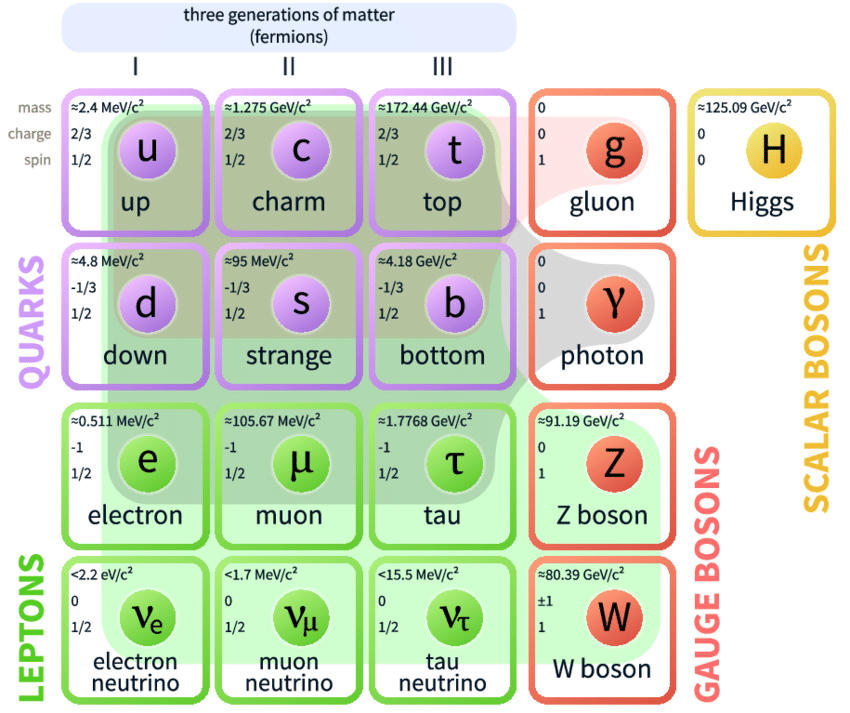
\includegraphics[width=0.75\textwidth]{figures/chapter_SM/SM}
            \caption{
                A schematic diagram of the Standard Model Particles seen in the scale of the experiment of the Large Hadron Collider.
            }
            \label{fig:SM}
        \end{center}
    \end{figure}

\section{Sucessful Prediction}
The Standard Model has many successes in the particle level, and it has made along with many successful predictions, these predictions include:
    \begin{itemize}
        \item existence of W boson %~\cite{}
        \item existence of Z boson %~\cite{}
        \item existence of the charm quark %~\cite{}
        \item existence of the top quark %~\cite{}
        \item existence of the Higgs boson %~\cite{}
    \end{itemize}

\section{Standard Model Measurement}
Many Standard Model properties has been measured under the ATLAS experiment, a summary plot on the cross section of the interactions can be found here:
%Summary plots 

    \begin{figure}[!htb]
        \begin{center}
            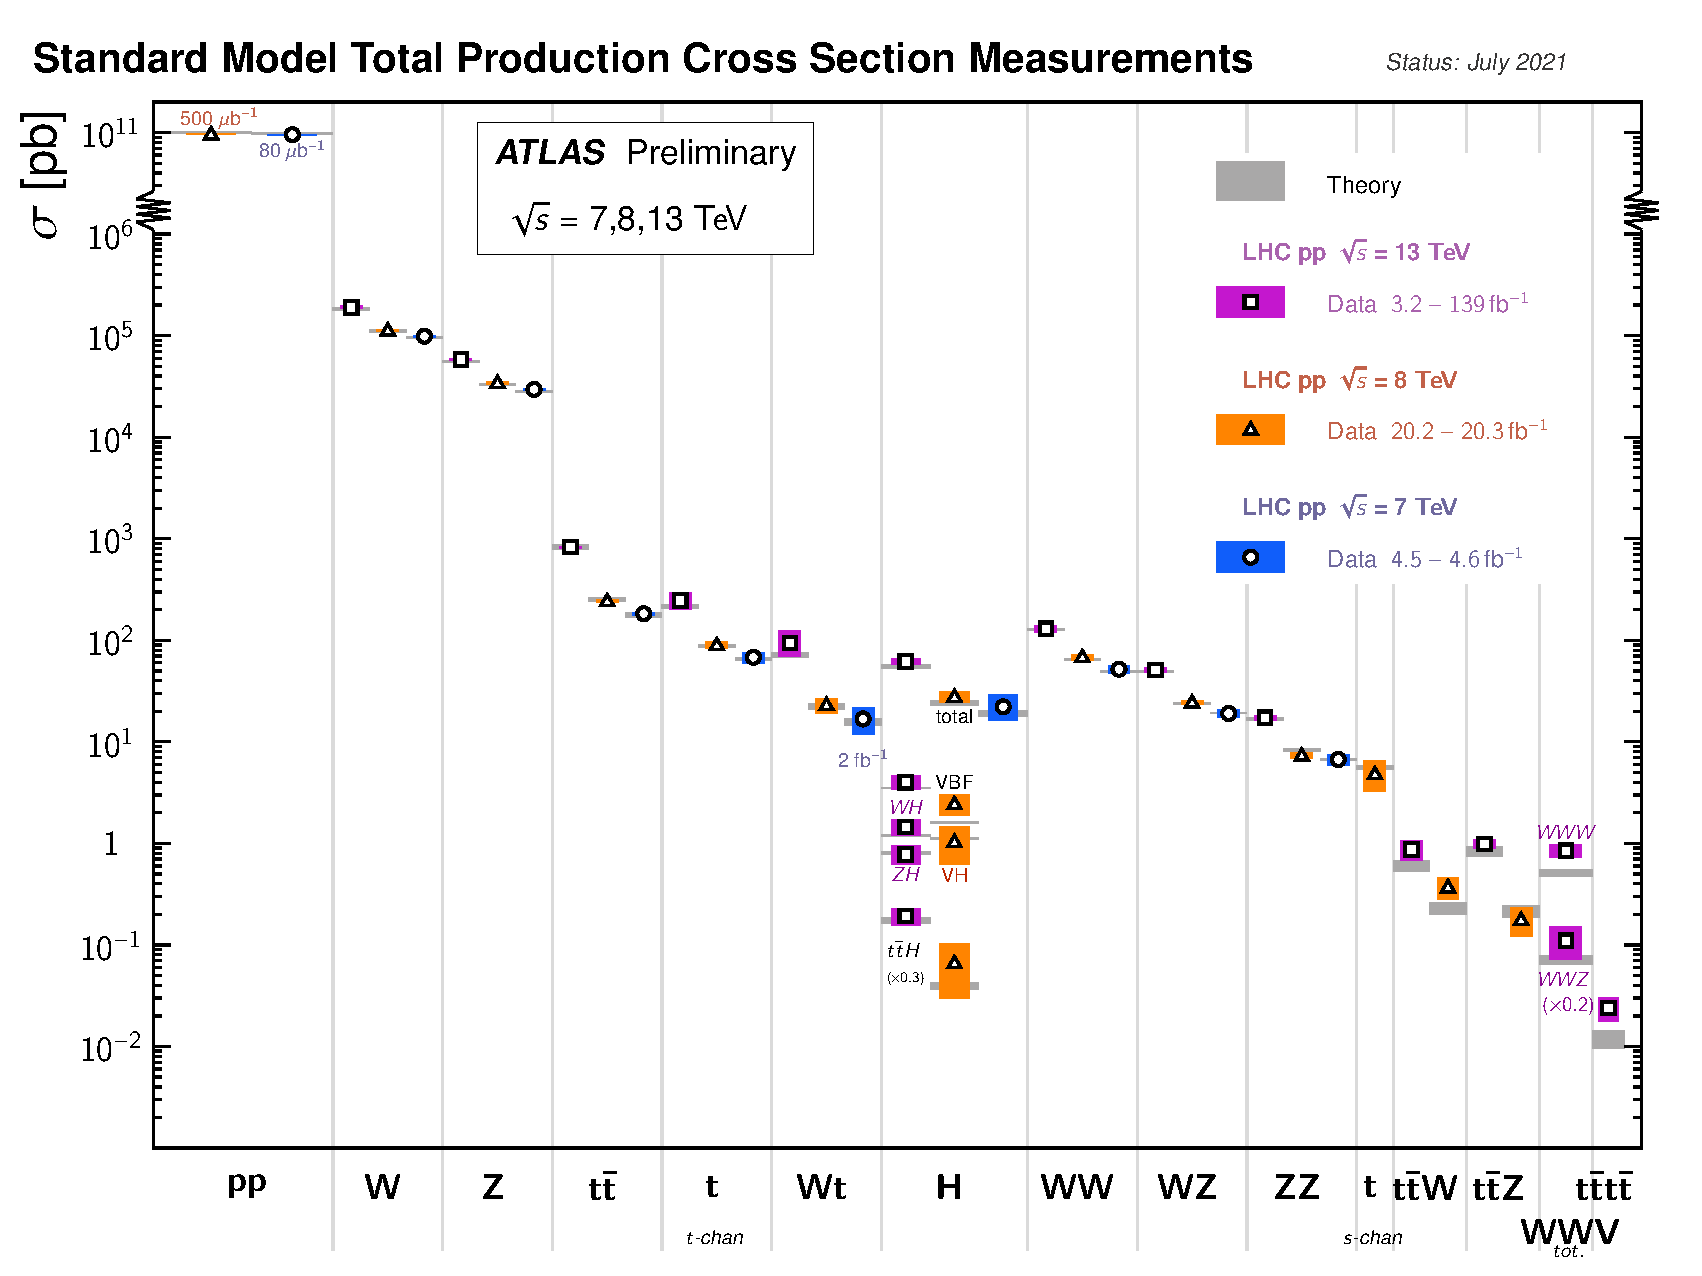
\includegraphics[width=0.75\textwidth]{figures/chapter_SM/SM_Measurement}
            \caption{
                A summary plot on the Standard Model cross-section measurements done by the ATLAS experiment~\cite{ATL-PHYS-PUB-2021-032}.
            }
            \label{fig:SM}

        \end{center}
    \end{figure}



\section{Unresolved Problems in the Standard Model}
The Standard Model of Particle Physics in its current forms has had many standing unresolved problems, leading to the belief that the model, despite its many sucesses is not the ultimate theory on fundamental particles. Here, some of the standing problems of the standard model and their proposed solutions are discussed.

\subsection{Gravity}
The Standard Model does not include gravity, one of four fundamental forces.     

\subsection{Naturalness}
Naturalness is the property in physics theory where the dimensionless ratio between the free parameters and the physical constants should be in the order of 1. When a physical theory takes either a very large or small value outside the order of 1, they are considered unnatural and unlikely to be the fundamental theory. 
The Standard Model shows many naturalness issues in different dimensions: 

\subsubsection{The Cosmological Constant Problem (Dimension 0)}
The Standard Model allows for a 0th dimension constant in its Lagrangian that would not break any of its symmetries. The constant would represent the vacuum energy density, and would account for the quantum fluctuation in vacuum. Under Zelokoch's calulations~\cite{zel1968cosmological}, the relations between the vaccum energy density and the cosmological constant of the Eintein's Equation is directly proportional as such:

\begin{equation}
    \rho_{vac}c^2=\Lambda c^4/8\pi G
\label{eq:cosmoconst}
\end{equation}

The cosmological constant is a well measured value in cosmology from the measurement of the expansion of the universe. The cutting off in either the Planck scale or the electro-weak scale in quantum field theory gives a theoretical prediction value of the vacuum expectation value. However these values do not match. In fact, the experimental measured value of \rho_{vac}is about 40-100 more order of magniture smaller than what's predicted in theory. The order of magnitude discrepancy poses the
biggest naturalness issue in the Standard Model~\cite{V2002}.

%Currently, there are proposition that the discrepany could be due to the fact that the neighboring universe is antropologically different than the whole universe[], or modifications could be done to the Einstein's Equation. But as these propositions violates other universal principle or theorems, none are satisfactory.


%In cosmology, it's known that there is a vacuum energy density that exist in the curvature of the universe that can be expressed as the cosmological constant in the Einstein's Equation. The Cosmological constant is measured with the expansion of the universe and would convert to a vacuum 
%In the 0th order, the cosmological constant as measured by experiment is between 40-100 more order of magniture smaller than predicted. 


\subsubsection{The Higgs Hierarchy Problem (Dimension 2)}
The Higgs hierarchy problem of particle physics describes the apparent large discrepany in order of magnitude between the electro-weak scale and the gravitational scale, the weak force is about $10^{24}$ greater than gravity. Its effect can be seen in the Higgs mass boson as the mass is 17 order smaller than would be expected by the Planck mass. 
A popular solution is quantum correction via supersymmetry, but as more phasespace for supersymmetry is being ruled out, this solution is increasingly unlikely to solve the problem. 

\subsubsection{The Strong CP Problem (Dimension 4)}
The Standard Model allows for a term that describes strong CP violation naturally:

\begin{equation}
    \mathcal{L}$_{QCD}$ \supset \theta$_{QCD}$\epsilon$_\mu\nu\rho\sigma $\mathcal{G}
$^{\mu\nu}\mathcal{G}$^{\rho\sigma} 

\end{equation}

However experimentally, CP violation is not observed, the neutron electro-dipole moment is exceptionally small, this therefore lead to where the free parameter in the term that describes the CP violation is either exceptionally small or zero. It's therefore unnatural for there to be such a term in the Lagrangian.
One well-known solution to the strong CP problem is the introduction of the Peccei-Quinn symmetry~\cite{PQSym}, under this solution, the new field will create a term that naturally cancels with the strong CP term. As under this solution, a new particle call the axion is predicted. Many experiments are on the look out for the particle, but it's never yet observed to-date. It's still up to future experimental result to showcase the validity of the theory.

\subsubsection{Neutrino Mass}
The Standard Model does not predict neutrino to have a mass, however that contradicts with experimental findings. Since neutrino oscillation is observed, there must be mixing between the neutrino mass state and flavor state, forcing the mass of neutrino to be a non-zero value. 

A minor extension to the Standard Model is needed to add in neutrino mass. Currently, there are two leading camps of \nu SM, one predicting neutrino as a Dirac field, like othee leptons in the Standard Model; and another that predicting it as a Majoranna field, in which the anti-neutrino and the neutrino is be the same particle. 

%\subsubsection{Triviality Problem}
%Landau pole + asymmototic freedom 


\subsubsection{Matter-Antimatter Asymmetry}
While the CKM matrix of the standard model does allow for matter-anti matter asymmetry, the measured value of the parameter is not large enough to account for the apparent observed matter-antimatter asymmetry in the universe. As the dominating amount of matter over antimatter is necessary to the formation of most galactic structure, stars and planets, this is a question that is in need to be answered.

\subsubsection{Flavor Problem}
The Stanadard Model does not provide an explanation to why there are 18 free parameters and why they take on the values that they do. The mass hierarchy of the quarks and the special quirkiness of the exceptionally large mass of the top quark are all questions not answered by the Standard Model. 


\subsubsection{Dark Matter}
In experiment, it is estimated that dark matter makes up about 85\% of all matter in the universe, but they are not accounted for in the Standard Model, making the Standard Model only a model that describes about 15\% of the known content of the universe in mass. More details are covered in the dark matter chapter. 

\section{Summary}
The Standard Model of Particle Physics has led to many breakthroughs in human's understanding on the fundamental building blocks of the universe and their dynamics. With the discovery of the Higgs boson in 2008, all the particles predicted by the model are found. Precise measurements are done on all of the 18 model parameters of the Standard Model in the LHC, rendering the collider a huge success in physics precision measurement history. However, despite its successful prediction and insight into existing physics, there remains many open questions and unanswered issues in the theory. All these discrepancies are little tears in the curtains giving us a previledged glimpse to a even more complete theory of truth out there.

In the next chapter, evidence and different hypotheses of dark matter will be examined in length, how it can be searched for in the Large Hadron Collider will be discussed. 

%\section{history}
    %Though the advancement in electrodynamics through the Maxwell's Equations and the progress of Special Relativity, Quantum Theory was re-development with the second quantization\footnote{} , path intergral through the study of Fock, Feynman and Paul Dirac, later led to the development of the quantum field theory.   
    %Paradigm of Quantum field theory, and is the basis where consequent theories in the standard model is based on. 

    %History that lead to the standard model
    %What is the standard model 
%\section{Symmetries}

%1. Electro-Weak theory
%    Q.E.D.
%    Dirac and the problem of annihilation of anti-particle lead to the second quantization, with work from 
%    Gauge theory
%    The unification of eletro-dynamic force and the weak force
%    The Higgs Mechanism / spontaneous symmetry breaking 
%
%4. Quantum Chromodynamics
%    Yang-Mill theory, non-abelian gauge groups. 
%5. Spontaneous Symmetry Breaking 

%-cannot describe atom level in QCD

    %* historically, how it was developed
    %* its sucesses, its predictions lead to W,Z, Higgs boson
    %* Neutrino oscillation or their non-zero mass

%Standard model is the corner stone and a starting point in the journey to particle discoveries, 

\chapter{Theory of Dark Matter}
\label{chapter:DM}
% add what does the different method excludes in the dark matter summary plot


\epigraph{\textit{One does not become enlightened by imaging figures of light, but by making the darkness conscious.}}{--Carl Jung}

%TODO: 1. Evidence Large scale structure of the universe
% 	   2. SUSY and long lived particle model and signature
%      3. 

	


\section{History}
\label{section:history}
    Dark matter is arguably one of the most solid evidence for Beyond-the-Standard-Model physics. In 1933, Fritz Zwicky first conceptualized the existence of a dunkle Materie ("dark matter") holding the galaxies to the cluster center and thus preventing them from flying apart ~\cite{Zwicky}. The proposition was later concurred by different findings by Horace W. Babcock ~\cite{Babcock} and Jan Oort ~\cite{oort}, among many others. The existence of such matter is also supported by evidence across different physics scales including the cosmic microwave background, and bullet cluster collision.

    Dark matter is known for interacting gravitationally and at most weakly (though recent evidence has shown weak scale interaction to be unlikely) with Standard Model particles . It does not interact electromagnetically or strongly. Its known properties does not match any known standard model particle. Very little is known about its composition and interaction mechanism. However, as dark matter makes up about 85\% of the matter in the universe ~\cite{Hinshaw_2013}, five times more than the ordinary matter covered in previous chapter. Its discovery would lead to a breakthrough in human understanding about the universe. Afterall, dark matter plays a major role in astrophysical mechanics, and has lasting effects in galactic cluster formation and the evolution of the universe. Without a proper understanding of dark matter and its composition, human understanding of the universe will be incomplete.

    Experiments and observations over the years have constricted some dark matter properties, but much of the physics is still remains a mystery. It is generally accepted that dark matter is a particle. Various ways are developed to study the mystery particle in telescope, earth based detector and colliders. In the LHC, dark matter can be studied through direct production. If dark matter can be produced in a laboratory, it will make probing many of its other properties possible. 

    In this chapter, evidence for dark matter is reviewed in~\ref{section:evidence}, dark matter and the current properties that restrict its nature will be covered in~\ref{section:properties}; section~\ref{section:candidates} reviews possible dark matter candidates. An overivew of search methods for dark matter is covered in~\ref{section:searches} ; highlights on the theoretical modeling approach used by the LHC of dark matter are discussed in~\ref{section:models}. Lastly, LHC dark matter search signatures are included in~\ref{section:signatures}.

\section{Evidence}
\label{section:evidence}

\subsection{Galactic Rotational Curve}
    The first proposition of dark matter in 1930s in the Coma cluster by Fritz Zwicky and others was later confirmed by further systemic galaxy rotational curve studies by Vera Rubin, Kent Ford ~\cite{Rubin} and Ken Freeman ~\cite{freeman}.  
    Following Zwicky's original argument, galactic clusters and galaxies are treated as stable systems of discrete particles in astrophysical scale. They are therefore govern by the Virial theorem:
% Rubin and Ford studied galaxy M31 region and found that different region moves at a different speed than expected of the mass of the galaxy
%

\begin{align}
\begin{equation}
     \langle T \rangle = -\frac{1}{2} \sum_{k=1}^{N} \langle F_{k} \cdot r_{k} \rangle
    \label{eq:virial}

\end{equation}
\end{align}


    The Virial theorem shows that the there is a direct correlation between the kinetic energy and potential energy in a particle system. In rotating galaxies, there is therefore a correlation between the velocity of the disk and the mass (through gravitational force) of the system. The correlation is as follows: 
    
     $$ v(r) \varpropto \frac{M(r)}{\sqrt{r}}, $$ where r is the distance from the center of the system.

    %Outside of the system, M(r) is a constant, the formula can be further simplified to:

    % \[ v \varpropto \frac{1}{\sqrt{r}} \], 

    However, in observation, it was found that the velocity distribution for many of these cluster does not follow the prediction by the Virial theorem. is close to constant to r in the outer rings ~\ref{M33_figure}.  A missing dark halo of dark matter that is not luminous is proposed to be a part of these galaxies.

\begin{figure}[!htb]
    \begin{center}
        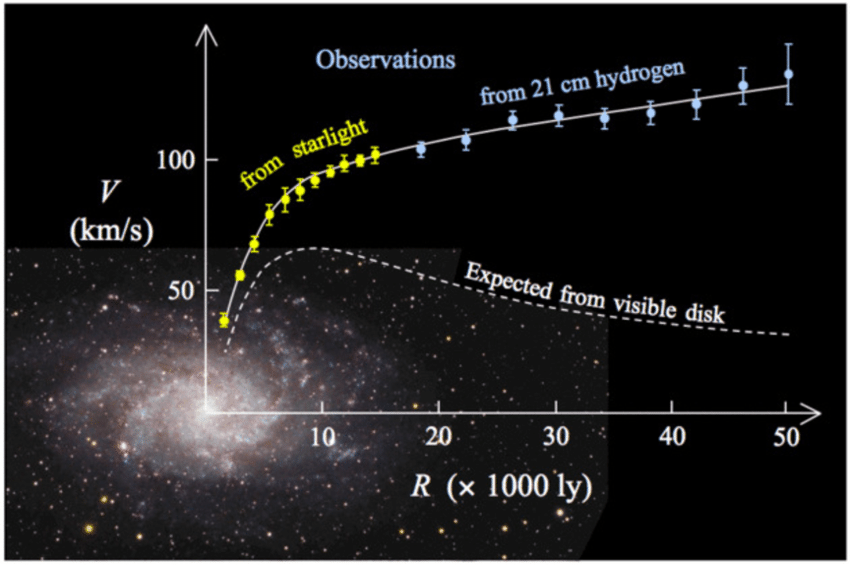
\includegraphics[width=0.75\textwidth]{figures/chapter_DM/M33-rotation-curve}
        \caption{
            Figure here shows the galactic rotational curve of M33, the expected rotational curve is shown in the dotted line. Experimental evidence observes behavior in the solid line.~\cite{M33}.
        }
        \label{fig:M33_figure}
    \end{center}
\end{figure}


\subsection{Gravitational Lensing}

    General relativity shows that massive objects would curve the space-time curvature around them. The details are capulated elegantly in the Einstein's Equation: 
%~\ref{eq:Einstein}: 

\begin{equation}
	R_{\mu \nu} - {1 \over 2}R \, g_{\mu \nu} + \Lambda g_{\mu \nu}= {8 \pi G \over c^4} T_{\mu \nu}, 
    \label{eq:Einstein}
\end{equation}

	In this equation, $R_{\mu \nu}$ is the Ricci curvature tensor, and R is the scalar curvature, together they form the Einstein tensor. $g_{\mu \nu}$ is the metric tensor, and $T_{\mu \nu}$ is the stress-energy tensor. This equation shows that the curvature of space-time is directly related to the mass and energy in that space. 	
	
	Consequentially, light rays that travel through the curved space-time around the massive object would therefore be bent. The effect mirrors that of angled lenses bending light rays due to a velocity difference of light rays across different media, and is called gravitational lensing. 

	There are different forms of lensing effect, roughly arranged by the strength of their effects. Strong lensing effect happens when bending of light result in either multiple images, a light ring or an arc, more typically observed around massive centers of galaxy clusters and galaxies; weak lensing usually involves statistical analysis of many objects over a large region; micro-lensing is detected when the effect only displays as an apparent change in the brightness of the source.

    Figure~\ref{fig:BulletCluster_figure} shows the bullet cluster collision of 1E 0657 -56. It is produced from the combination of gravitational lensing and x ray telescope imaging. The red part of the diagram denotes ordinary matter and the blue part reflects dark matter. In the cluster collision, ordinary matter bend light around them and became luminous from the collision, captured by x-ray imaging; the blue part shows a part of the clusters that did not interact and light up in the collision via gravitational lensing. This is a strong evidence for the existence of non-luminous matter in the clusters.

\begin{figure}[!htb]
    \begin{center}
        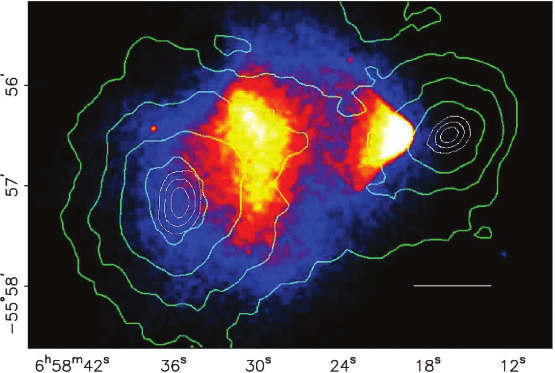
\includegraphics[width=0.75\textwidth]{figures/chapter_DM/BulletCluster}
        \caption{
			Bullet cluster (1E 0657-56) showing two colliding galaxy clusters, the part in red came from x-ray image by Chandra, highlighting normal matter distribution; the part in blue came from gravitational lensing. ~\cite{BulletCluster}.
        }
        \label{fig:BulletCluster_figure}
    \end{center}
\end{figure}


\subsection{Cosmic Microwave Background}

    In the beginning of the universe, ordinary matter and dark matter all exist in a hot plasma soup with frequent interaction between charged particles and photons through Thomson scattering. There comes a very important period in the universe called the recombination period, where the expansion of the universe has cool the plasma soup enough that charged particles began to form neutral atoms. Photons stopped scattering on the charged particles and went on unhindered. Due to red
shifting effect, they form a microwave background of the universe that can still be observed today. This is the Comic Microwave Background. 
This original background is nearly a black body and is therefore very uniform, but there exists small temperature variations. The variation can be decomposed into an angular power spectrum, as shown in Figure~\ref{fig:CMB_figure}

Due to the different interaction between dark matter and ordinary matter with photon and each other, simulation shows that different dark matter and ordinary matter make-up of the universe would result in different angular spectroscopy shape. 

Study from Planck on cosmic microwave background Figure~refgives a clear composition and percentage abundance of dark matter. Dark matter is not only an essential part of the universe, its composition is approximately 5 times as large as ordinary matter. Giving evidence that dark matter makes up the majority of the universe. 
%\figure planck 

\begin{figure}[!htb]
    \begin{center}
        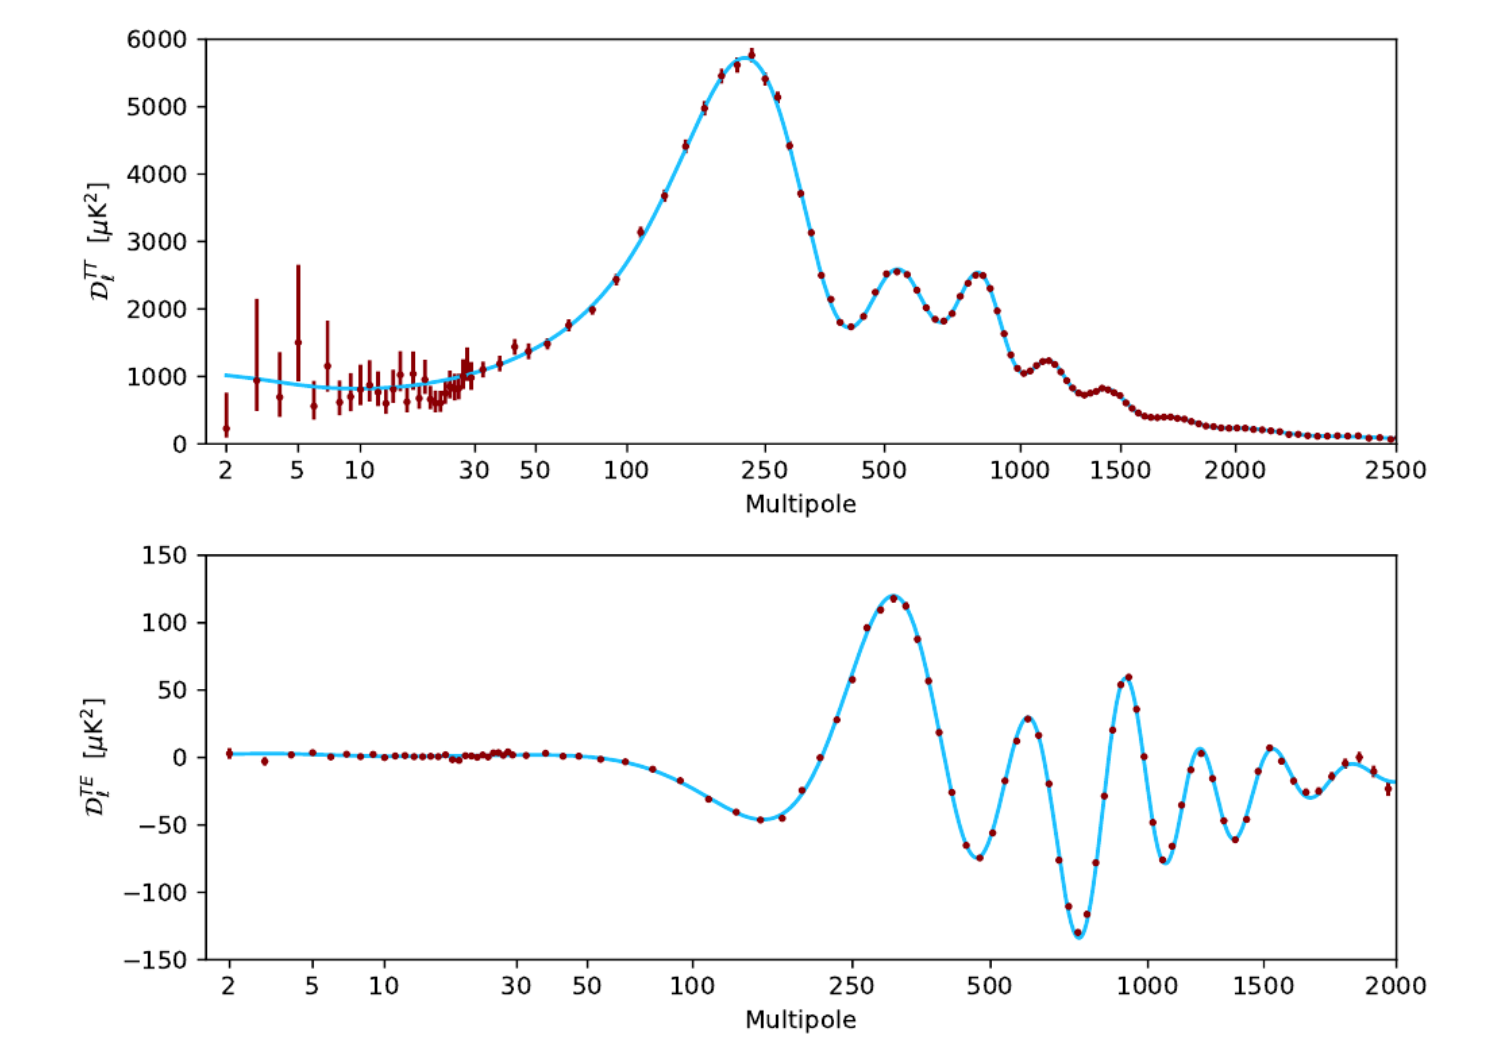
\includegraphics[width=0.75\textwidth]{figures/chapter_DM/CMB-angular-power-spectrum}
        \caption{
			The Cosmic Microwave Background power spectrum measured by Planck.~\cite{CMB}.
        }
        \label{fig:CMB_figure}
    \end{center}
\end{figure}


%\subsection{Large Scale Universe Structure}
%Gravity has a deterministic effect on how the universe is formed, and therefore affects the large scale structure of the universe. The existence of dark matter 
%https://www.forbes.com/sites/startswithabang/2020/10/02/ask-ethan-can-dark-matter-really-explain-the-universes-structure/?sh=5b37659b3b06


\section{Properties}
\label{section:properties}
While dark matter itself has never been directly observed, many studies in the cosmological, astrophysical and particle scale has constrained much of its properties. In this section and the remaining thesis, the following properties of dark matter will be assumed along with its justifications.

\subsection{Dark}

Dark matter got its name from its little to no interaction with light compared to ordinary matter in cosmological observation. Collision of the bullet cluster has also greatly constrained its interaction with itself.  
It is taken that it will not interact with collider detector and its interaction with ordinary matter would be rare in the energy scale of the LHC. 

\subsection{Long Life Time}

As dark matter is seen today in evidence across difference scales (see section ~\ref{section:evidence}). It is assumed to have a long life time since its creation in the early universe. Many theoretical model of dark matter require a $Z_{2}$ symmetry (such as the R parity of supersymmetry). This prevent dark matter particles from decaying into lighter Standard Model objects. In most experimental searches today, it is be treated as a single particle that does not decay further into other detectable SM particles. ~\cite{boveia2018dark}


\subsection{Interact Gravitationally}
Current evidence (see section ~\ref{section:evidence}) suggests that dark matter is massive (i.e. it interacts gravitationally). However, there is no consensus on the mass on the individual parts of dark matter. Current theoretical candidates of dark matter roughly be split into two camps: cold dark matter and hot dark matter. The former group believes that dark matter is made of object massive enough to be non-relativistic; the latter group hold the opposite view. 

\subsection{Cold}
In cosmology, hot/cold refers to the mass of an object. Only objects relatively low in mass would be affected relativistically. Different assumption of the relativistic mass of dark matter has great impact on the galaxy formations and its distribution. From most simulation results, dark matter is taken to be non-relativistic by most physicists and will be assumed for dark matter candidate searched for in the rest of the thesis. 

\subsection{Low Self-Interaction}
Dark matter is believe to have little to no self interaction, Mixed X-ray, optical and gravitational lensing study on the merging galacy cluster 1E-657-65 has restricted its self interaction limit to below $\sigma \over m < 1.25 cm^{2} g^{-1}$ (68\% confidence)~\cite{randall2008constraints}. 
 
%\subsection{Single Particle}
%While there are many composite dark matter models being proposed these days, dark matter is still taken to be a single kind in most effective model/simplified model building for experimental searches. 

\section{Candidates}
\label{section:candidates}

There exist a wide range of candidates for what dark matter could be. In here, a few possible particle candidate of dark matter are outlined here. 

\subsection{Sterile Neutrino}
Standard model does not predict that neutrino has a mass, however, that contradicting with experimental finding and is therefore a problem of the standard model. By replacing right-handed neutrinos in the standard model with gauge singlet fermions that has no interaction other than mixing with normal neutrinos, sterile neutrino is formed by theoretical models. Tuning parameters such its interaction rate with normal neutrino, mass and mixing angle, sterile neutrino can be a possible candidate for dark matter, as it can lead to a right
density of dark matter with stability consistent with the scale of the universe. ~\cite{dodelson1994sterile} They are searched for in radiator experiments such as the Daya Bay \cite{an2014search, wong2017search} and in scintillator experiments like DANSS. ~\cite{alekseev2018search}

% Mass and range  mass keV scale, currently sterile neutrino mass is unknown and therefore can be either hot or cold

%Daya Bay Collaboration, F. P. An et al., “Search for a Light Sterile Neutrino at Daya Bay,” Phys. Rev. Lett. 113 (2014) 141802, arXiv:1407.7259 [hep-ex].
%1310.8642
\subsection{Axion}
Another exisitng problem in the standard model is the strong CP problem. The strong CP problem points to the unnaturalness of CP symmetry observed in neutrons charge distribution measurement. This gives an exceptionally small value to the term that govern strong CP violation in the Standard Model, which is unnatural. The problem can be solved by introducing an additional axion particle and its associated fields to the standard model. ~\cite{peccei1977cp} With the proposition of such field, the CP violation term in strong interaction will be cancelled out naturally, thereby giving an explanation to the unnaturalness to the experimental value. 
The axion proposed is a dark matter candidate, as its calculated life time is much greater than the age of the universe and it shares many properties with the known profile of dark matter. Recent experimental finding from the XENON1T and shows anomalies that could be signs of axions. ~\cite{aprile2020excess}
%ADMX mass mu eV
%https://arxiv.org/pdf/2105.01406.pdf

%Xenon Collaboration, E. Aprile et al,. "Excess Electronic Recoil Events in XENON1T", Phys. Rev. D 102, 072004 (2020), arXiv: 2006.09721


% Non-particle candidates
%\subsection{Modified Newtonian Gravity}
%\subsection{MACHOs}

\subsection{Weakly Interacting Massive Particle (WIMP)}
A very attractive candidate for dark matter is called the weakly interacting massive particle(WIMP). It appears naturally with many Beyond-the-Standard-Model theories that aim to solve other physics problems, including theories of supersymmetry with R-parity and some extra dimensional theory. 
In the study of dark matter in cosmology, it is frequently assumed to be a thermal relic. Thermal relic dark matter is in thermal equilibrium with ordinary matter in the early universe. In thermal equilibrium with ordinary matter, it gets produced and annihilated at the same rate. There comes a point in the universe called freezing out, where the expansion of the universe cools the particle bath and produce temperature lower than possible to produce enough energy statistically for dark matter to
be produced given certain dark matter mass. Dark matter production from ordinary matter ceased. As the universe further expanse, it becomes more difficult for dark matter to find each other to be annihilated to form ordinary matter. Dark matter abundance is locked at this point and remained unchange until today. 
Using this model and the current measured abundance of dark matter in our current universe, the self annihilation cross section of dark matter is $ \langle \sigma \cdot v \rangle \simequal 3 \cdot 10^{26}cm^{3} s^{-1}$. This annihilation cross section scale matches many prediction made in supersymmetry theories. Many Beyond-the-Standard-Model theories, such as SUSY, the Universal Extra Dimension Model, and the little Higgs all predict a particle with known dark matter properties and self interaction rate of the same scale. This is known as the WIMP miracle. ~\cite{Dev_2014}

%\Figure WIMP miracle


\begin{figure}[!htb]
    \begin{center}
        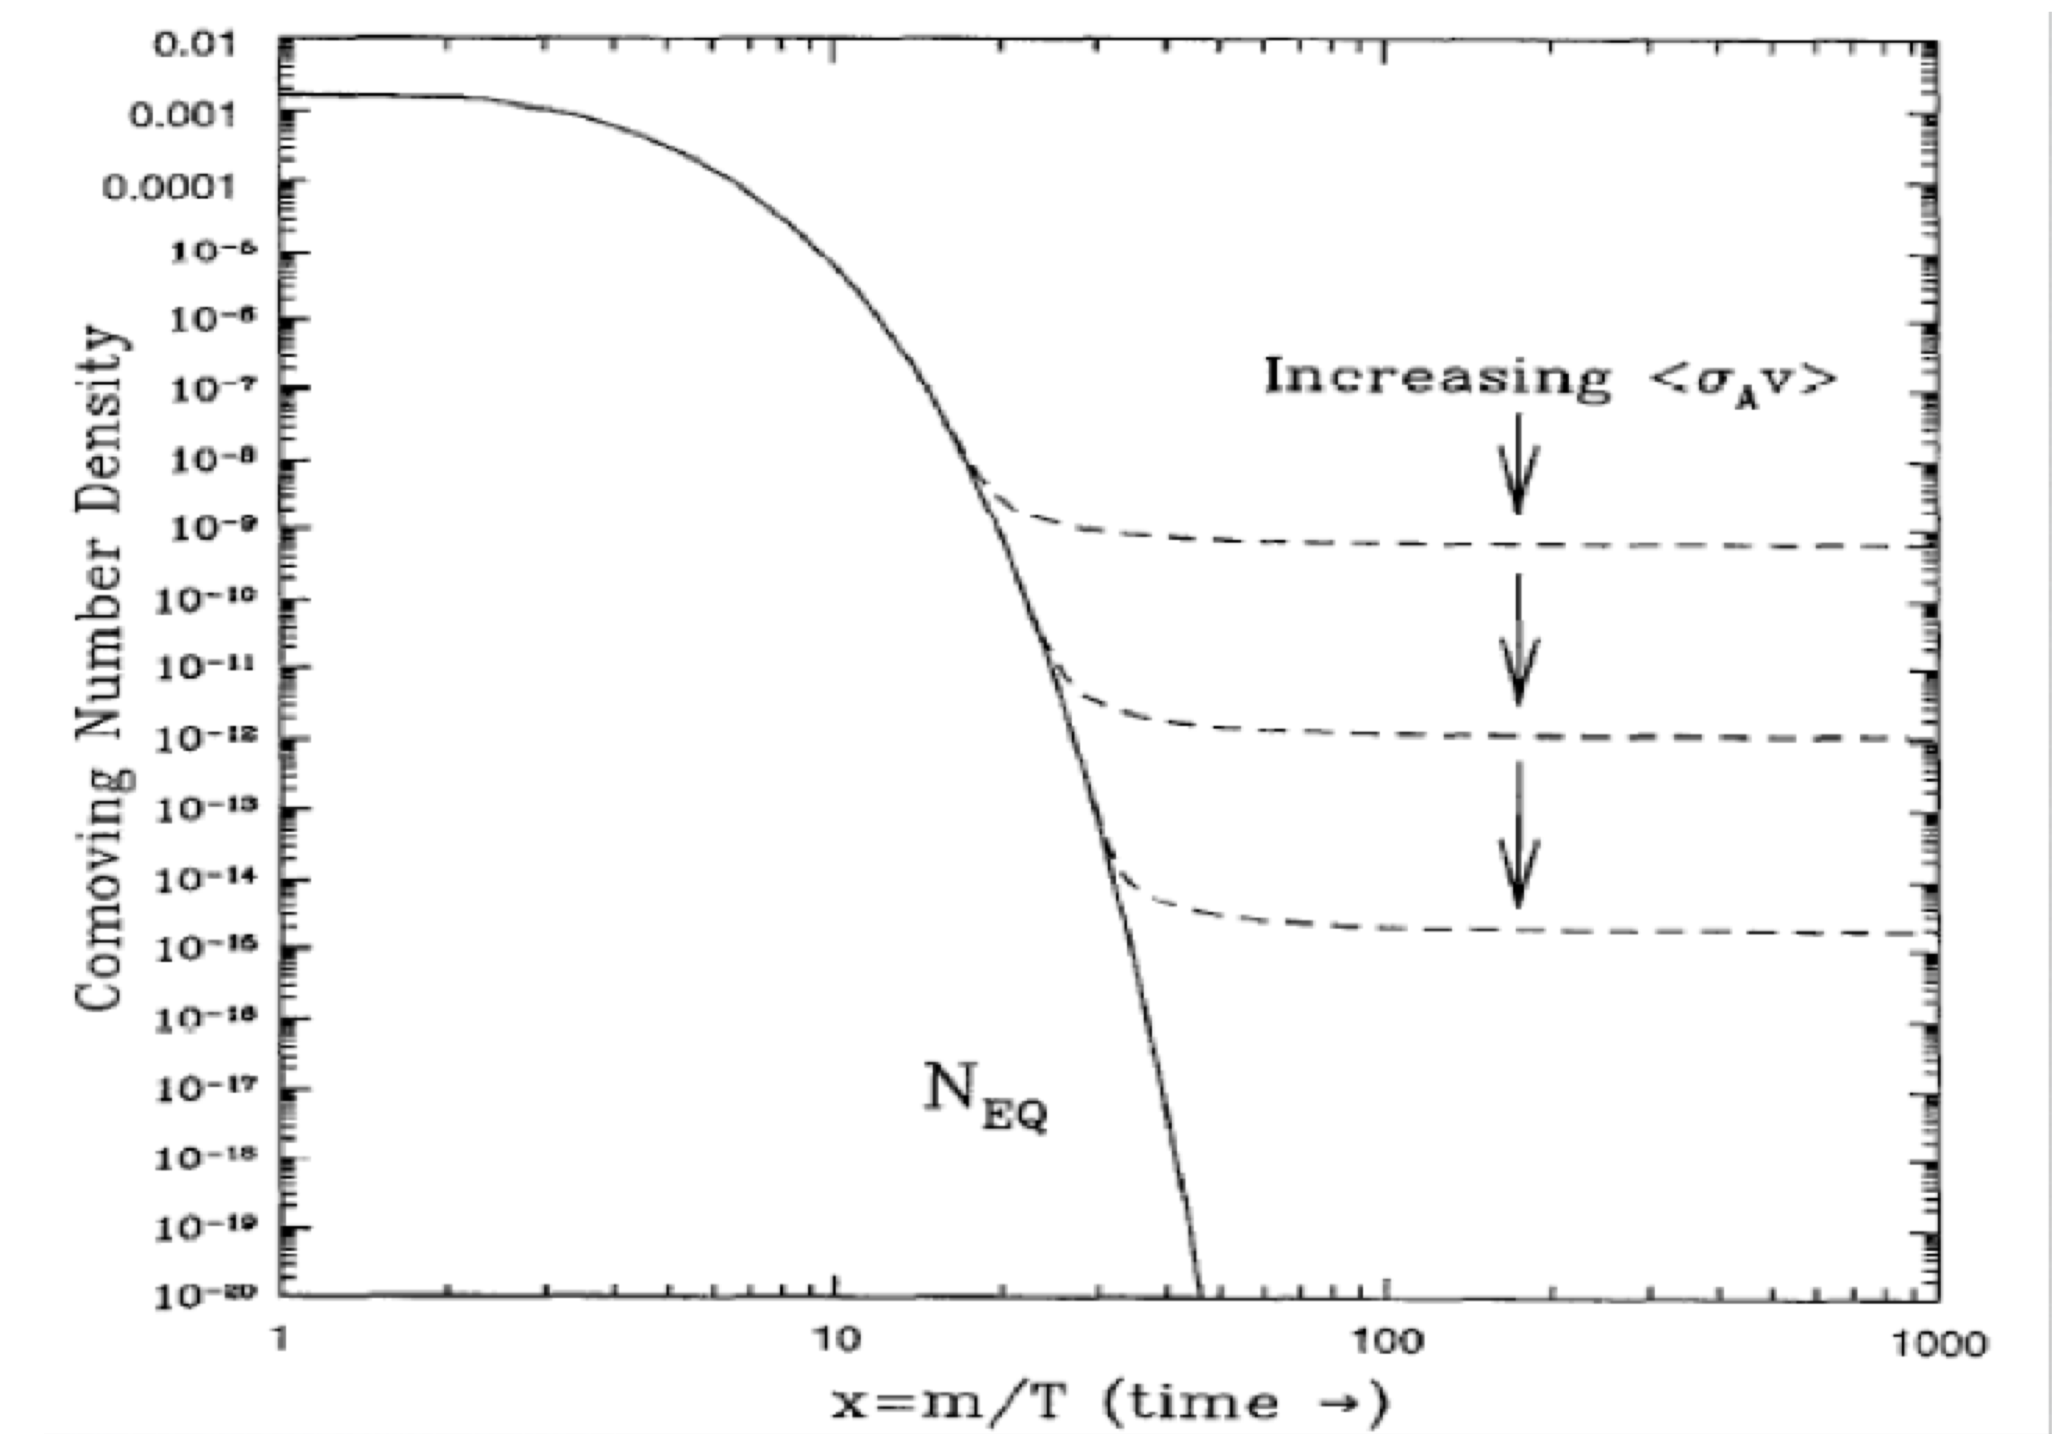
\includegraphics[width=0.75\textwidth]{figures/chapter_DM/WIMP}
        \caption{
		Solid line here shows the change in the densitiy of dark matter in an expanding unverse. In the early universe, the solid line is horizontal, indicating the time when dark matter production and annihilation is equal. The line gradually fall with increase of time when production rate began to decrease with the universe expansion. Later as the universe further expands, the annihilation stops as well and dark matter gets freezes out to different density level with different assumed self interaction annihilation rates.~\cite{WIMP}.
        }
        \label{fig:WIMP_figure}
    \end{center}
\end{figure}


 

%P.S. BHUPAL DEV, ANUPAM MAZUMDAR, & SALEH QUTUB, FRONT.IN PHYS. 2 (2014) 26
%https://indico.cern.ch/event/473000/contributions/1993414/attachments/1209863/1764345/tait-Aspen.pdf

%https://www.particlebites.com/?p=7004
%https://www.forbes.com/sites/startswithabang/2019/02/22/the-wimp-miracle-is-dead-as-dark-matter-experiments-come-up-empty-again/?sh=5ebc59f46dbc

\section{Experimental Search Overview}
\label{section:searches}

Traditionally the search for dark matter is split into different experimental categories sorted by the different detection methods from different dark matter/normal matter interactions. 

\begin{figure}[!htb]
    \begin{center}
        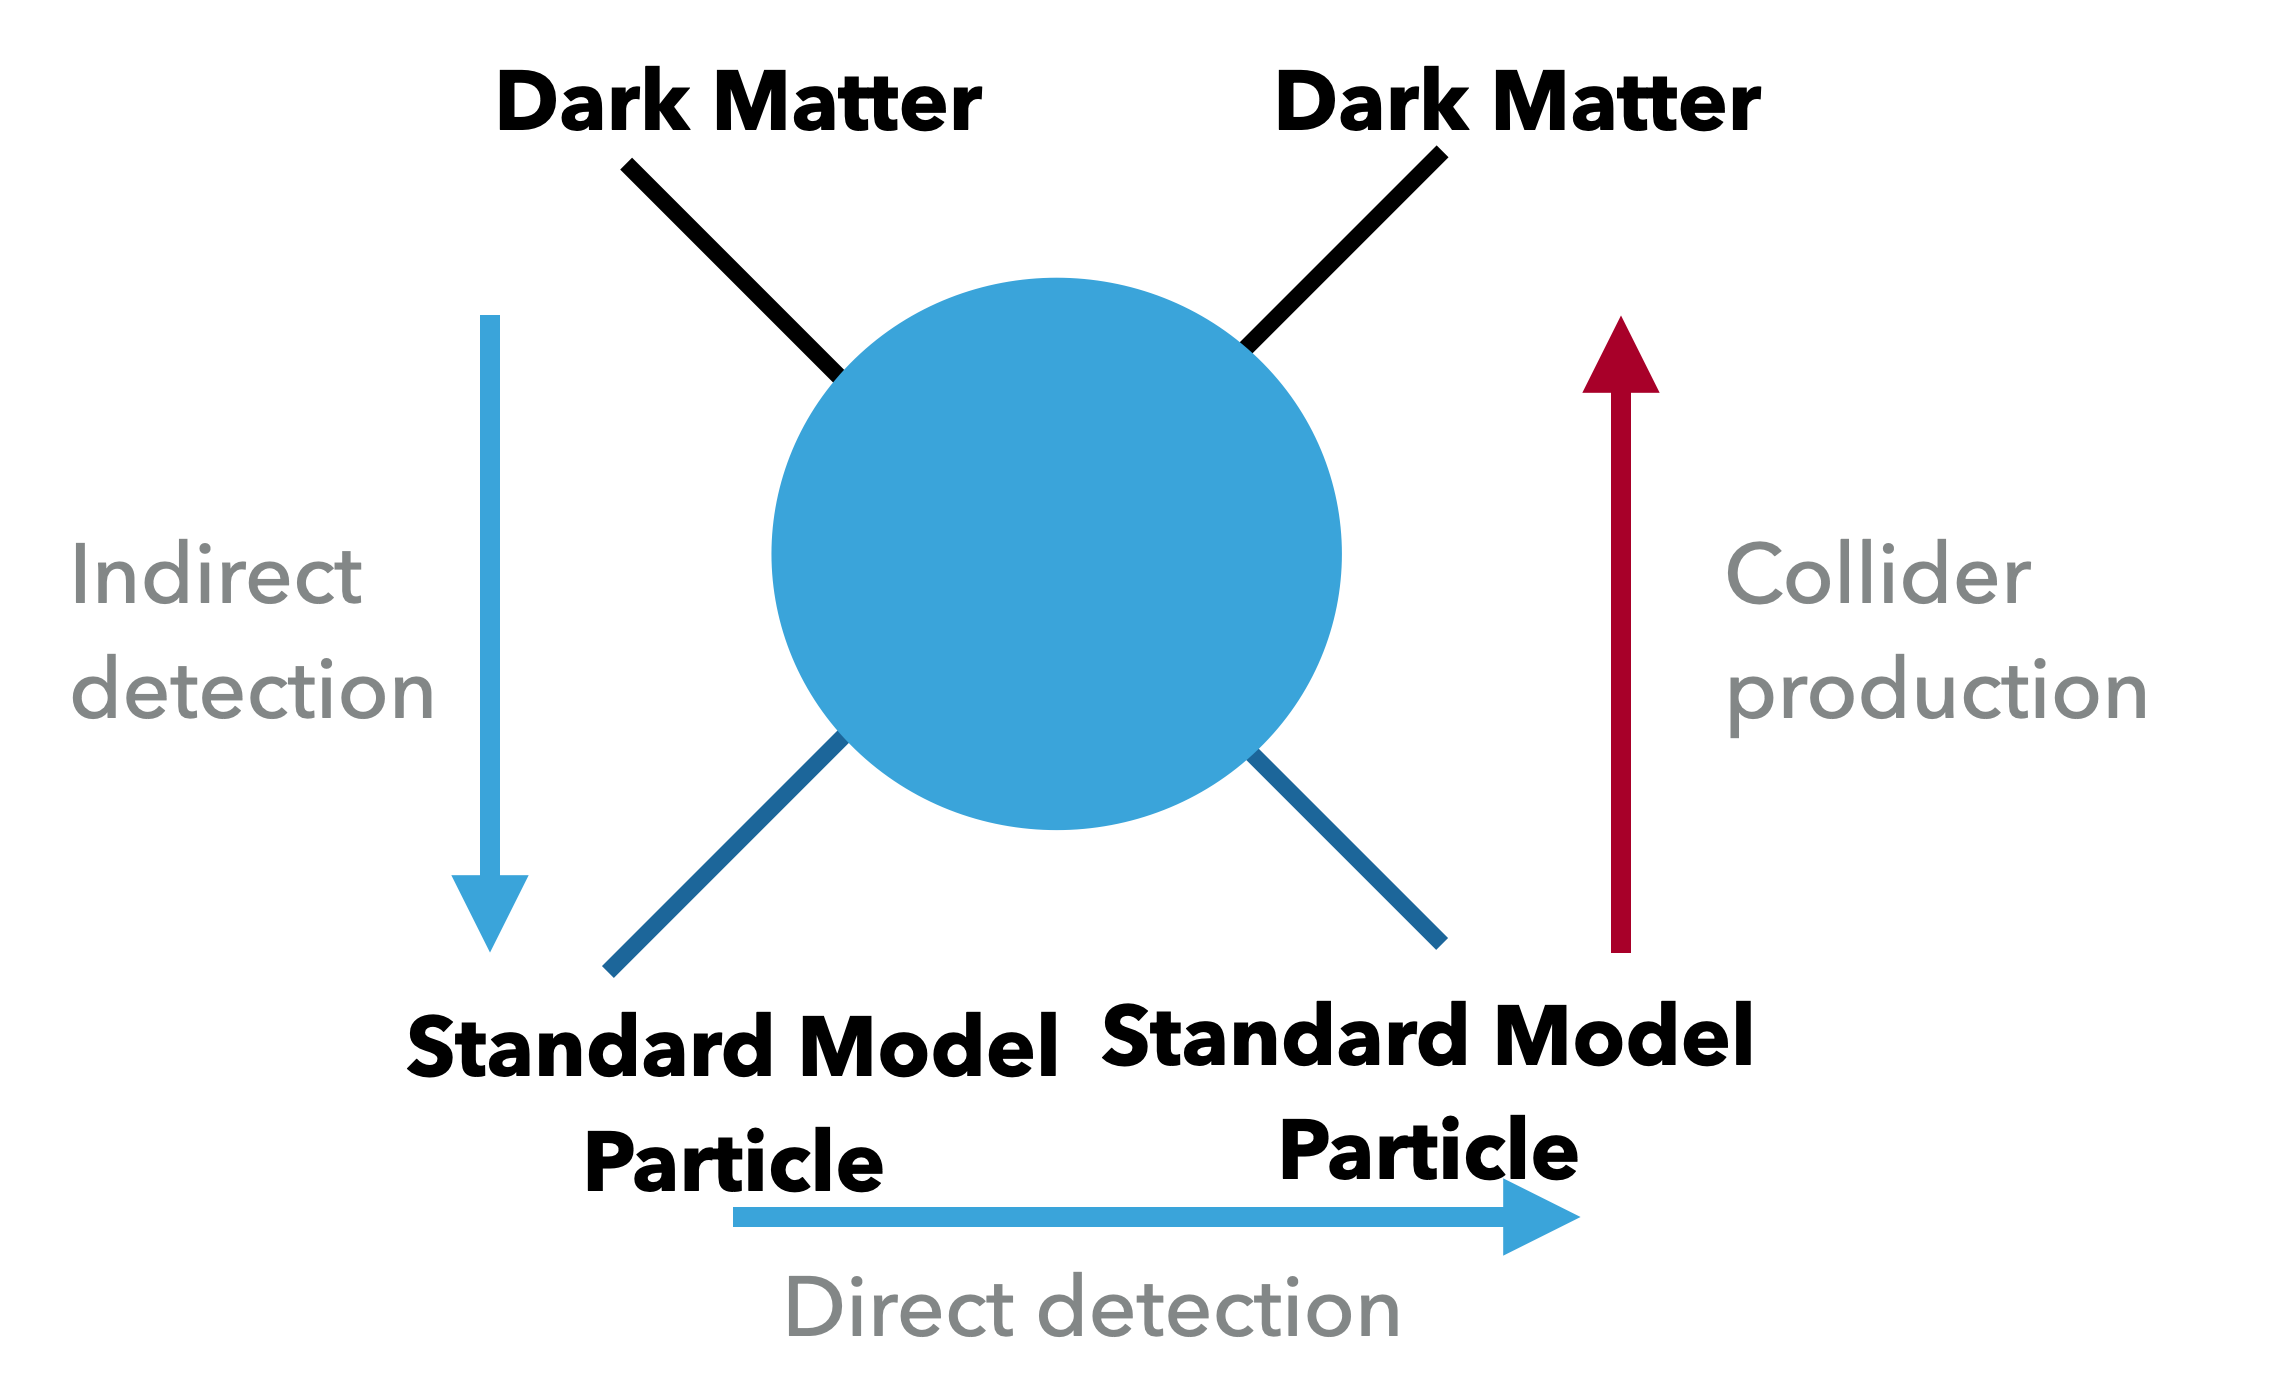
\includegraphics[width=0.75\textwidth]{figures/chapter_DM/Interaction}
        \caption{
			Schematic cartoon showing the different dark matter detection methods facilitated by different interactions thus signatures. 
        }
        \label{fig:interaction}
    \end{center}
\end{figure}

\subsection{Direct Detection}
Dark matter is believed to travel through the universe and passes through the eath. Assuming weak interaction between dark matter and Standard Model nucleons, dark matter can be detected directly with different target objects. 

\[ R \propto N \rho \chi \langle \sigma_{\chi } N \rangle \]

There are different experiments that uses different material and targets different dark matter masses.
Notable experiments include LZ ~\cite{mckinsey2016lz},   Xenon1T ~\cite{aprile2020excess}, SuperCDMS ~\cite{Agnese_2016}, CRESST ~\cite{Angloher_2014} and DAMA ~\cite{Bernabei_2008}. 

As more experiments has excluded much of the theory model phasespace, many of the experiments now faces the challenge of the neutrino floor in low mass dark matter search, which is where neutrino background began to dominate signal region. 



\subsection{Indirect Detection}
Indirect detection looks for annihilation Standard Model product of dark matter. It looks for interaction in places where matter is dense enough to interact, usually in center of galaxies and stars. Experiments include FermiLAT ~\cite{albert2017searching} and H.E.S.S. ~\cite{aharonian2006hess}


\subsection{Collider Production} 
    In the Large Hadron Collider, dark matter can be studied by being directly produced from Standard Model particles.

\section{Theoretical Models in LHC Searches}
\label{section:models}

While there exist a wide range of speculation on the identity of dark matter, the use of LHC as a dark matter searching tool constrains a unique set of dark matter candidate accessible phenomenologically. 
Focusing phenomenologically observable and interpretability for a wide range of theoretical models, different modeling approaches are used to develop benchmark models searching for dark matter in the LHC.
Sorting by an ascending degree of completeness, the literature will review different approaches and models of dark matter used in the LHC.


\begin{figure}[!htb]
    \begin{center}
        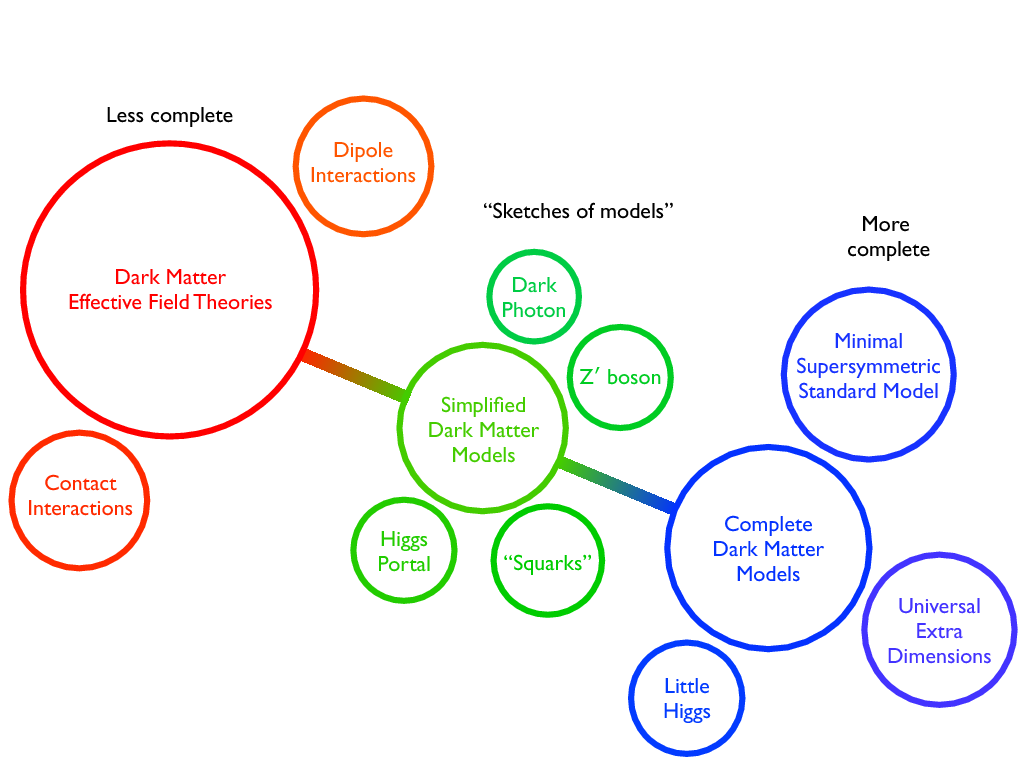
\includegraphics[width=0.75\textwidth]{figures/chapter_DM/Model}
        \caption{
			Colored Scheme showing dark matter modeling approach from more simplistic (left) to more complete models (right).  ~\cite{Abdallah:2024101}.
        }
        \label{fig:Model_figure}
    \end{center}
\end{figure}



\subsection{Simple Portal Models}
The simplest kind of models are simple extensions to the standard model. In these models, dark matter is mediated either through the Higgs or the Z Boson. As the Z portal models are constrained by LEP and DD experiments, dark matter that are mediated through a heavier version of Z boson ( the Z') and additional scalar is also searched for. 

\subsection{Effective Field Theory}
The effective field theory approach condenses a wide range of complete models to simplified versions by focusing on what is experimentally accessible. High mass mediator particles in complete theories as a contact operator. High energy correction and details are integrated out for "effectiveness". All kinematically accessible observables are described by a Lorentz structure and a rate parameter. 
This approach allow for the easily measured experiment values and a framework for a wide range of complete models to be probe with few experimental model search. However, the model has a singularity and is not valid for when the interaction momentum transfer is close to that of the mediator mass. In the LHC, a truncation method is used to bound the events simulated Monte Carlo events below this limit ~\cite{Busoni_2014}.

\subsection{Simplified Model}
The problem in effective field theory can be resolved with the simplified Model appraoch. The contact interaction in EFT is turned into mediator particle s-channel/t-channel exchanges in simplified model. With the price of an increased number of parameters, simplified models can provide the full mechanics of a particle interaction and usually come with more details. 
Simplified models of dark matter in the LHC do not break the global and gauge symmetries of Standard Model, the Lagrangian terms are Lorentz invariant and predicts at least a dark matter candidate that fullfills the properties described in the previous section. 
Some simplified dark matter model used in the LHC include the Two-Higgs Doublet Model (2HDM), where Higgs or a non-standard model exotic Higgs could serve as a mediator to dark matter; other examples include dark photon or a kinetically mixed Z' dark matter model. 
Other than these, simplified model in supersymmetry such as the Phenomenological Minimal Supersymmetric Standard Model (pMSSM) which reduces the over 100 parameters of complete model of Minimal Supersymmetric Standard Model to 19 parameters, predicts candidate dark matter like particles, predicts neutralino as a natural dark matter candidate. 
In addition, other gauge or gravity mediated SUSY theory predicts gravitino as a dark matter candidate. 
% pMSSM Assumes no sources of CP violation Beyond-the-Standard-Model and no flavor-changing neutral currents, and retains uni- versal couplings and masses for first- and second-generation superpartners. %CatDog Antonio DM summary paper.  

\subsection{Less-simplified models}
The LHC dark matter working group is moving towards less simple models with more phenomenological details.
%\subsection{Long-Lived Particle Models}

A detailed list of models used by the LHC by both the CMS and ATLAS can be found in this reference ~\cite{Abercrombie_2020}.

\subsection{The LHC Dark Matter Benchmark}
\label{sec:LHCDM}
The dark matter benchmark from the LHC uses the effective field theory approach. (See section for more detail on this appraoch) It uses contact interaction operator as the basis of the theory model building blocks. This way, the model can be reduced to a handful of experimentally measurable qualities for more complete theory model interpretations. 
In the dark matter benchmark of the LHC, it extends the Standard Model by an additional U(1) symmetry, and assumed dark matter along with some Stanard Model particles are all charged under this. A new gauge boson can thereby facilitate interaction between the standard model and dark matter field. 

The dark matter mediator can either be an axial vector or a vector, the corresponding lagrangians are as such:

\[ \mathcal{L}_{vector}= g_{q} \sum$_{q=u,d,s,c,b,t}$ Z'_{\mu}\bar{q}\gamma^{\mu}q + g_{\chi}Z'_{\mu}\bar{\chi}\gamma^{\mu}\chi \]


\[ \mathcal{L}_{axial vector}= g_{q} \sum$_{q=u,d,s,c,b,t}$ Z'_{\mu}\bar{q}\gamma^{\mu}\gamma^{5}q + g_{\chi}Z'_{\mu}\bar{\chi}\gamma^{\mu}\gamma^{5}\chi \]

This is also applicable to leptons, under this calculation the minimal parameters of the model is reduced to {g_{q}, g_{\chi}, m_{\chi}, M_{med}}. 

Similar arguments can be made for the lepton couplings. 

On ATLAS, these models are generated in the event generator with NLO+PS accuracy with the POWHEG generator, the product goes through parton showering at PYTHIA8 with detector simulation from GEANT4. 


\section{Experimental Signature in the LHC}
\label{section:signatures}

\subsection{Mono-X signature}
    This describes the type of dark matter search where an invisible dark matter is produced directly in the LHC and is "observed" in the detector as missing transverse momentum.
    Dark matter is known to interact only very weakly with normal matter, and thus is assumed to not leave a trace in the LHC detector. When events are produced through proton-proton collision along the z-axis in the LHC, the momentum of all objects along the transverse plane to the z-axis is always zero. Therefore, when an event has missing transverse momentum recoiling against another visible object, the signature would possibly be dark matter.
This class of analysis is named by the standard model object that dark matter recoil against. Mono-jet, mono-Higgs, mono-Z are a few analyses done this way. 

\subsection{Di-object Signature}
    Dark matter can also be searched for without the production of the dark matter particle. The simplified models that predicts dark matter in the mono-X analyses predicts effective mediator particle between standard model particle with dark matter. These effective mediator particles can be directly searched for through via decay back into standard model object. As the process is distinct from any known Standard Model particle processes, an excess of events Beyond-the-Standard-Model prediction for
    such a mediator process could be evidence for dark matter in the LHC. 
These di-object search include dijet, dilepton, diphoton searches. 
In recent years, new techniques such as the trigger-level-analysis and channels that has an additional initial state radiation objects are being pioneered. These result in a search phasespace much greater than the traditional program and greatly extended the of the richness of the LHC serach program.

\subsection{Supersymmetric Signature}	

\subsection{Long-Lived Particle Signature}


The Signature used for this analysis 

\chapter{The Large Hadron Collider And the ATLAS Detector}
\label{chapter:ATLAS}

All data used in this thesis is taken from the ATLAS experiment~\cite{ATLAS:1999vwa} of the Large Hadron Collider(LHC)~\cite{Bruning:782076} in the European Organization of Particle Physics(CERN).

CERN is the largest research organization on particle physics in the world. (See Figure~\ref{fig:LHCOnBorder}for a schematic map) The laboratory was built in the 1950s as a joint European effort to advance particle physics. It includes a total of 23 member states to date. Many major physics discoveries were made at CERN. Most notably, the discovery of the W, the Z boson~\cite{hioki1982does}, and the first man-made antihydrogen atom~\cite{hioki1982does}. In 2012, a boson of mass 125 $GeV/c^{2}$ was discovered, it is believed that it matches the
profile of the long sought after Higgs Boson particle~\cite{chatrchyan2012observation}, which gives an explanation to the origin of mass of matter in the universe. The site with 2660 on-site personnels and 12,400 users from over 70 countries also produced many technological derivatives outside of scientific discoveries. In particular, the World Wide Web was first built at CERN~\cite{berners1994world}.

This chapter presents the hardware and software apparatus in the LHC at CERN used to collect and produce the datasets for the later analyses.
The working and the layout of the LHC, the machine used to accelerate protons and monitor its collisions is presented in Section~\ref{LHC}; the ATLAS detector, the apparatus used to collect proton-proton collision data is described in Section~\ref{ATLAS}. Lastly, the triggering chain: the hardware and software collecting strategy is presented in Section~\ref{trigger}.

\begin{figure}[!htb]
    \begin{center}
        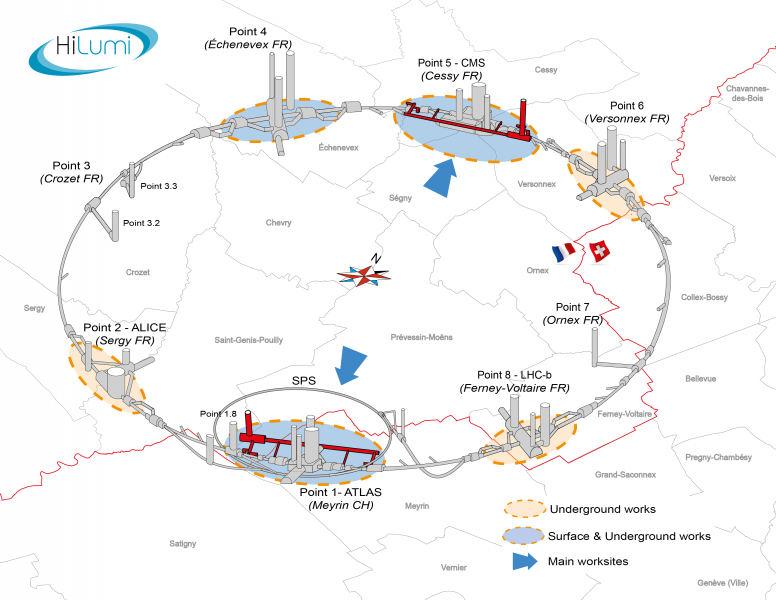
\includegraphics[width=0.75\textwidth]{figures/chapter_ATLAS/LHCOnBorder}
        \caption{
            This figure shows where the CERN is located geographically, across the border between France and Switzerland~\cite{Bruning:782076}.
        }
        \label{fig:LHCOnBorder}
    \end{center}
\end{figure}

\section{The Large Hadron Collider}
\label{LHC}

The LHC is located on the France-Switzerland border. Its main ring is a 27 kilometers tunnel that is 175 meters underground. It's mainly used to collide protons. Lead-lead collisions and proton-lead collisions are also done for a few weeks in each data-taking year. 

The collider was a planned successor to the Large Electron-Positron (LEP)(209 GeV collision) and the Tevatron collider (1TeV) in Fermilab. Since the last two experiments, the community converged on a consensus of an O(10)TeV scale proton collider with the main physics goal to probe electro-weak scale Higgs boson, beyond-the-Standard-Model physics, and further Standard Model measurement studies. The LHC was born.

The LHC reuses the same tunnel as the LEP experiment, with some major modifications were done to the tunnel for the upgrade: to achieve higher center-of-mass energy and to collide proton-proton instead of electron-positron, the angular velocity of the particle colliding would need to be raised. The existing magnet from the LEP experiment was therefore replaced to make way for more powerful cryogenic-based super-conducting magnets to bend higher speed particles. In addition, as the LHC uses a proton-proton beam rather than an electron position in the LEP, an extra beam pipe was required. This is due to the fact that the proton beams collisions could not share the same beam pipe as the position-electron beams in the LEP. The radio frequency system is also modified in the upgrade to the LHC to allow for acceleration of the two separate beams in the LHC.

After the upgrade, the main ring of the LHC allows for particle collision to happen in four main intersection points. These four points are directly inside the four major experiments of ATLAS~\cite{ATLAS:1999vwa}, CMS~\cite{CMS:2006myw}, LHCb~\cite{lhcb2001technical} and ALICE~\cite{Cortese:519145}: 

ATLAS and CMS are general-purpose detectors, data collected from these experiments are used for studies including Standard Model measurement, Higgs property measurement as well as exotic and new physics searches. The similar but slightly different detector structure between the two experiment allow for crosschecks and validation of physics results. ALICE is optimized to study strong physics in the quark-gluon plasma generated from lead-lead collisions. LHCb is a forward detector that specializes in b(bottom quark)-physics measurement. Studies on the bottom quark done in LHCb measures CP violation parameter and could help better understand matter-antimatter asymmetry of the universe. 

In addition to the four major experiments, the LHC currently hosts four more experiments. LHCf looks for forward particles that originate from cosmic radiation~\cite{Adriani:926196}. FASER is an experiment in search of long-lived exotic particles with a lifetime beyond the ATLAS detector~\cite{Ariga:2651328}. MoEDAL, which sits in the cavern of LHCb, looks for the magnetic monopole or highly ionizing stable massive particles (SMP)~\cite{Pinfold:1181486}. TOTEM shares the CMS interaction point; it measures the total
cross-section, diffraction process and elastic scattering processes of particles in the proton collisions~\cite{TOTEM:2004hps}. 

The LHC is designed to operate at a maximum center-of-mass energy of 14 TeV. Protons that get collided at the different interaction points go through many stages before collisions. 

In the following sections, some technical terms related to LHC operation will be discussed. Different parts of the LHC from proton production, proton acceleration to proton collision in the center of the ATLAS detector is also covered.

\begin{figure}[!htb]
    \begin{center}
        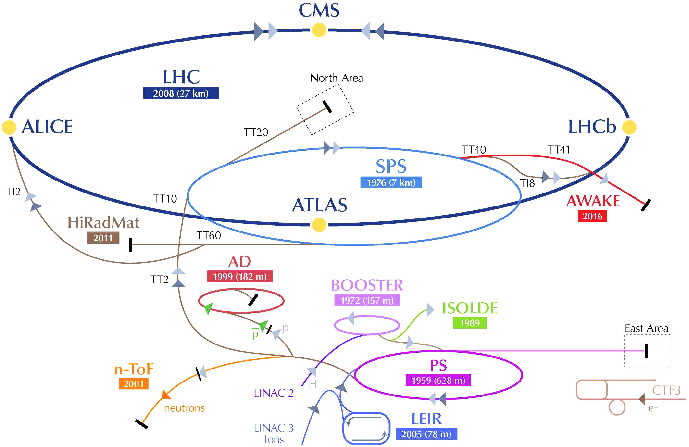
\includegraphics[width=0.75\textwidth]{figures/chapter_ATLAS/LHCAcceleratorComplex}
        \caption{
			This figure shows the accelerator complex of CERN, featuring the experiments and injection chain of the LHC~\cite{Marcastel:1621583}.
        }
        \label{fig:CERNAcceleratorComplex}
    \end{center}
\end{figure}

\subsection{Luminosity}
The instantaneous luminosity is a measure of how many events can be produced under certain detector conditions. It's directly related to the event rate of different processes under production.   
The quantity is given as the following:

\begin{equation}
    L = \frac{F \cdot N^{2}_{p} n_{b} f_{\lambda}}{4\pi\epsilon \beta^{*}}
\end{equation}


\begin{equation}
    \rightarrow = \frac{N_{\textrm{proton in beam 1}} \cdot N_{\textrm{proton in beam 2}} \cdot \textrm{Beam Crossing frequency }}{\textrm{Beam overlap Area}}
\end{equation}

In the formula above, $N_p$ is the number of proton in each beam, $n_{b}$ is the number of bunches per beam, f is the frequency of the beam traveling around the collider, and $\beta^{\*}$ is the beam cross-sectional size at the injection, $\epsilon$ is the beam emittance, F is the beam crossing angle.

The LHC was built to have a peak luminosity at L=$2 \cdot 10^{34}cm^{-2}s^{-1}$, but in most of Run II, it has a nominal value of $10^{34}cm^{-2}s^{-1}$.

While the instantaneous luminosity is a measure of LHC performance in operation, integrated luminosity, denoted by $\mathcal{L} = \int L dt$ is a measure of the amount of data taken over time.

While an increase in instantaneous luminosity increases the event rate in the experiment, it also increases the pile-up, which is multiple occurrences of interactions that happened simultaneously as the target events. Pile-up cleaning will therefore become an increasingly important task as the LHC instantaneous luminosity goes up.

\subsection{Proton Production}
The protons that collide in the LHC came from hydrogen in gaseous form. The electrons are stripped out from getting sent through an ion source. Protons formed are grated to make sure they are in the same direction before being sent off to the injection chain for acceleration. 

\subsection{The Injection Chain}
The acceleration of protons after their production is done through the so-called injection chain. It mainly consists of a series of pre-acceleration steps through the different linear booster and booster rings. As the speed and energy of the particle are effectively restricted by both the accelerator ring size as well as magnet strength in a cyclotron accelerator, a dedicated series of smaller rings in ascending order in size are used to accelerate the beam to a higher energy level before the LHC ring.

The protons first go through a linear accelerator named LINAC2 to be accelerated to 50 MeV. After the acceleration, they enter a synchrotron ring called the Proton Synchrotron Booster, the protons are accelerated to 1.4 GeV at this stage. Subsequently, they are injected into the Proton Synchrotron(PS). The PS accelerates the protons further to 26 GeV and is injected into the Super Proton Synchrotron(SPS), the protons are then further accelerated to 450 GEV and passed onto the LHC ring in \textit{proton bunches}.

These booster rings are existing structures from previous collider experiments~\cite{ATLAS:1999vwa}.

\begin{figure}[!htb]
    \begin{center}
        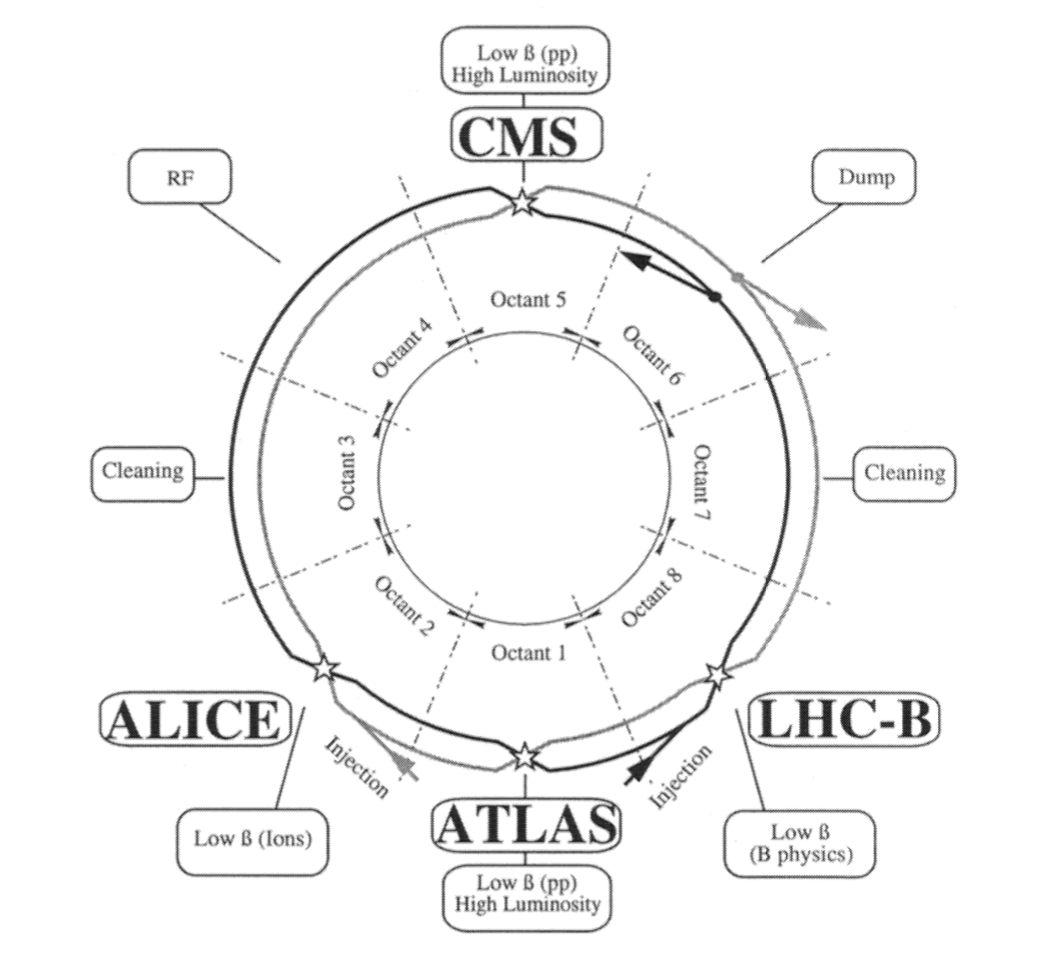
\includegraphics[width=0.75\textwidth]{figures/chapter_ATLAS/LHCRing}
        \caption{
			This figure shows the different parts of the two LHC rings along with its features~\cite{Pettersson:291782}.
        }
        \label{fig:perterson}
    \end{center}
\end{figure}

\subsection{The Radio Frequency Cavities}
After the injection to the LHC, the protons will be further ramped up in energy. Located in IP4 of the LHC main ring, the radio frequency(RF) cavity of the LHC performs the acceleration of particles in the ring. The cavity oscillates its electric field at a fixed 400MHz rate, which accelerates the incoming well-timed protons. In Run II, Protons that arrive in the LHC are accelerated from the 450 GeV injection energy to 6.5 TeV in 10 million loops around the LHC, which takes approximately 20 minutes. Other
than accelerating protons, the cavity also modulates the protons' energy: the slowed protons are accelerated and fast one decelerated. They are grouped into proton bunches.

\subsection{The Beam Dump}
The beam dump of the LHC is located in IP6 of the ring. It is designed to abort the beam for when an issue occurred in the LHC to prevent further damage. 

\subsection{The Magnets}
The magnet systems in the LHC provide a way to control the proton beam after its injection from the SPS. The magnets of the LHC serves a couple of different purposes on the LHC: they bend the proton beams for them to stay on the circular cyclotron tunnels; they also focus and align the beam for collision for maximal interaction rate. Due to the high bending power needed, the main ring of the LHC uses NbTi superconducting magnets.  A supporting cryostatics system cools the magnets down to 1.9K
for the superconducting functionalities. The main dipole system is shown to be able to provide a magnetic field of up to 8.4T under this condition. There are a couple of different kinds of magnets along the
LHC, each providing a different function in maintaining the beam for particle collision. The field quality can be summarized by the harmonic multipole analysis: 

\begin{equation}
 B_{total} = B_y+ iB_x  = B_1\sum_n(b_{n} + i a_{n})(Z/R_{r})^{n-1}
\end{equation}

where $B_y$ is the dipole field in the y-direction, $b_{n}$ and $a_n$ is the multipole coefficients, Z is a complex paramter that describes the coordinates of the magnet, $R_{r}$ is the reference radius, the index of n, refers the to the poles of the magnet field, where n=1 refers to the dipole file, n=2 refers to the quadrupole field and so on. 

\subsubsection*{The Main dipole magnets}
The main magnet is a dipole magnet that bend the proton beams to make them stay on track in the circular tunnels. It can also be used to control the separation of the beam as it enters and exit from different parts of the main ring. 
The LHC has two beam pipes for each proton beam going in the opposite direction from the other. The Magnet has a twin-aperture system that allows it to bend both proton beams together. Figure~\ref{fig:dipole} shows the cross-section of the dipole magnet. 

\begin{figure}[!htb]
    \begin{center}
        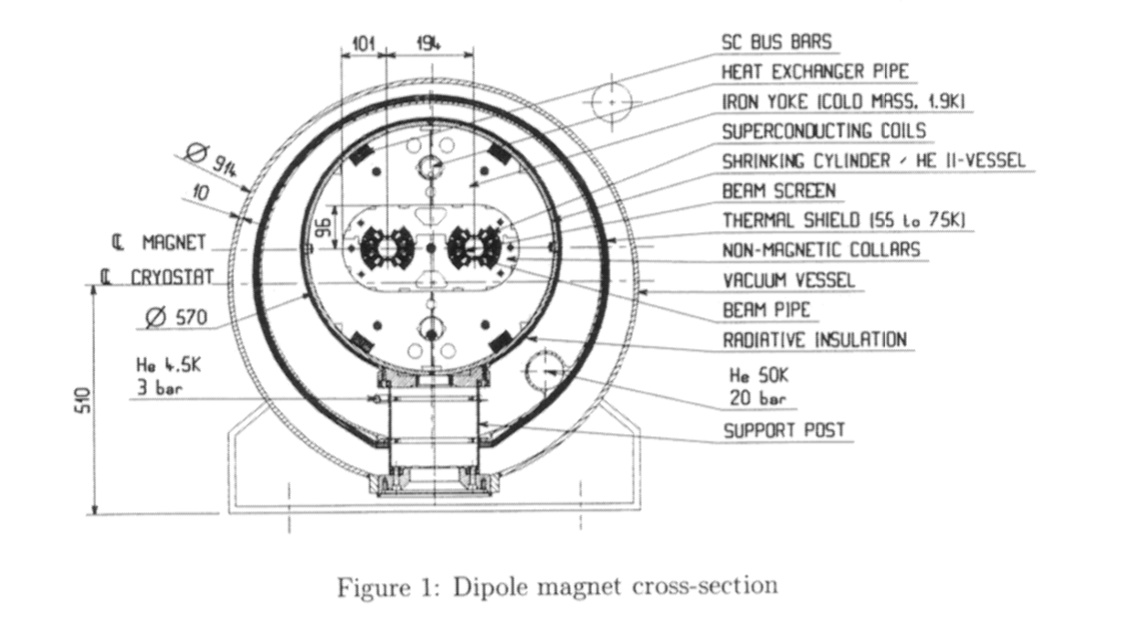
\includegraphics[width=0.75\textwidth]{figures/chapter_ATLAS/DipoleMagnets}
        \caption{
        The cross-section of the dipole magnet~\cite{Bruning:782076}.
        }
        \label{fig:dipole}
    \end{center}
\end{figure}

\subsubsection*{The Quadrupole Magnet}
The Quadrupole magnets are used in the LHC to focuses and defocuses the proton beams for collision. They are built in a way that is much like the main dipole, where single quadrupole magnet is capable of bending two proton beams. Figure~\ref{fig:quadrupole} shows a cross-section of the quadrupole magnet. 

\begin{figure}[!htb]
    \begin{center}
        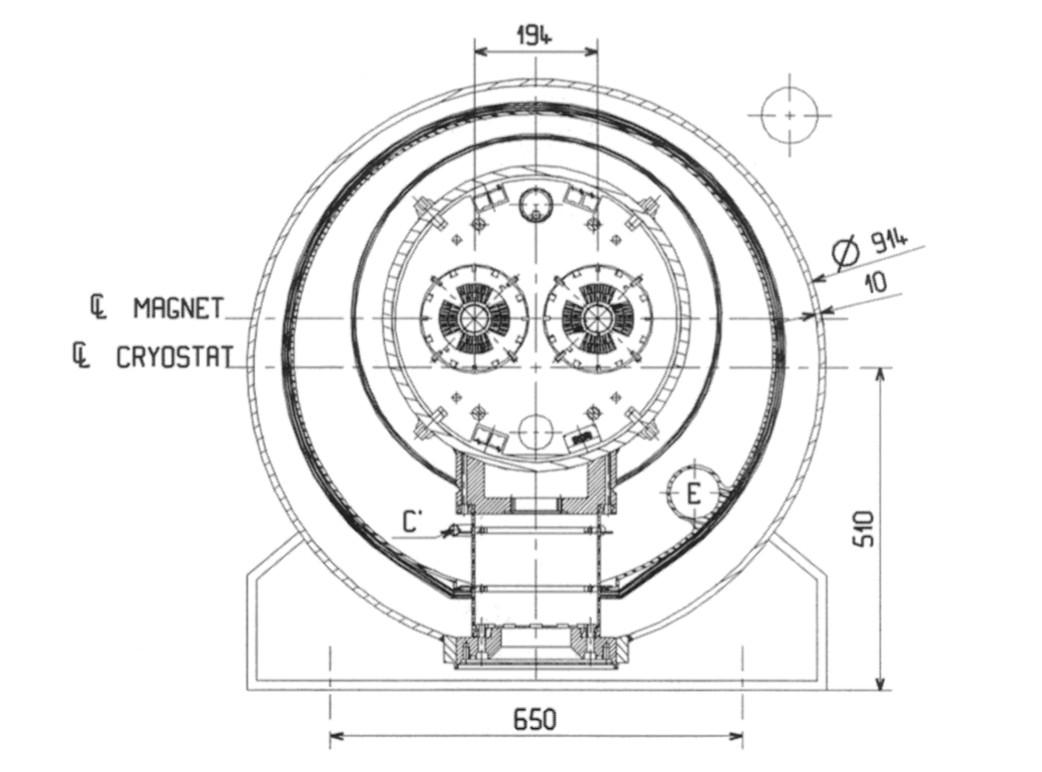
\includegraphics[width=0.75\textwidth]{figures/chapter_ATLAS/QuadrupoleMagnets}
        \caption{
            The cross-section of the quadrupole magnet~\ref{Bruning:782076}.
        }
        \label{fig:quadrupole}
    \end{center}
\end{figure}

\subsubsection*{The Sextupole and Dipole Corrector Magnet}
In addition, there are corrector magnets that correct for the field error of the main magnets mentioned above. More design details can be found in the conceptual design report of the LHC~\ref{Bruning:782076}.

\section{The ATLAS Detector}
\label{ATLAS}
The ATLAS detector is a general-purpose detector. It is the summation of a series of detector systems each produces different tracks to a particle. The ATLAS detector has a special emphasis on the muon system, as the dimuon final state was a main channel for the Higgs discovery. In the following sections, different parts of the detector will be discussed in detail. 

\begin{figure}[!htb]
    \begin{center}
        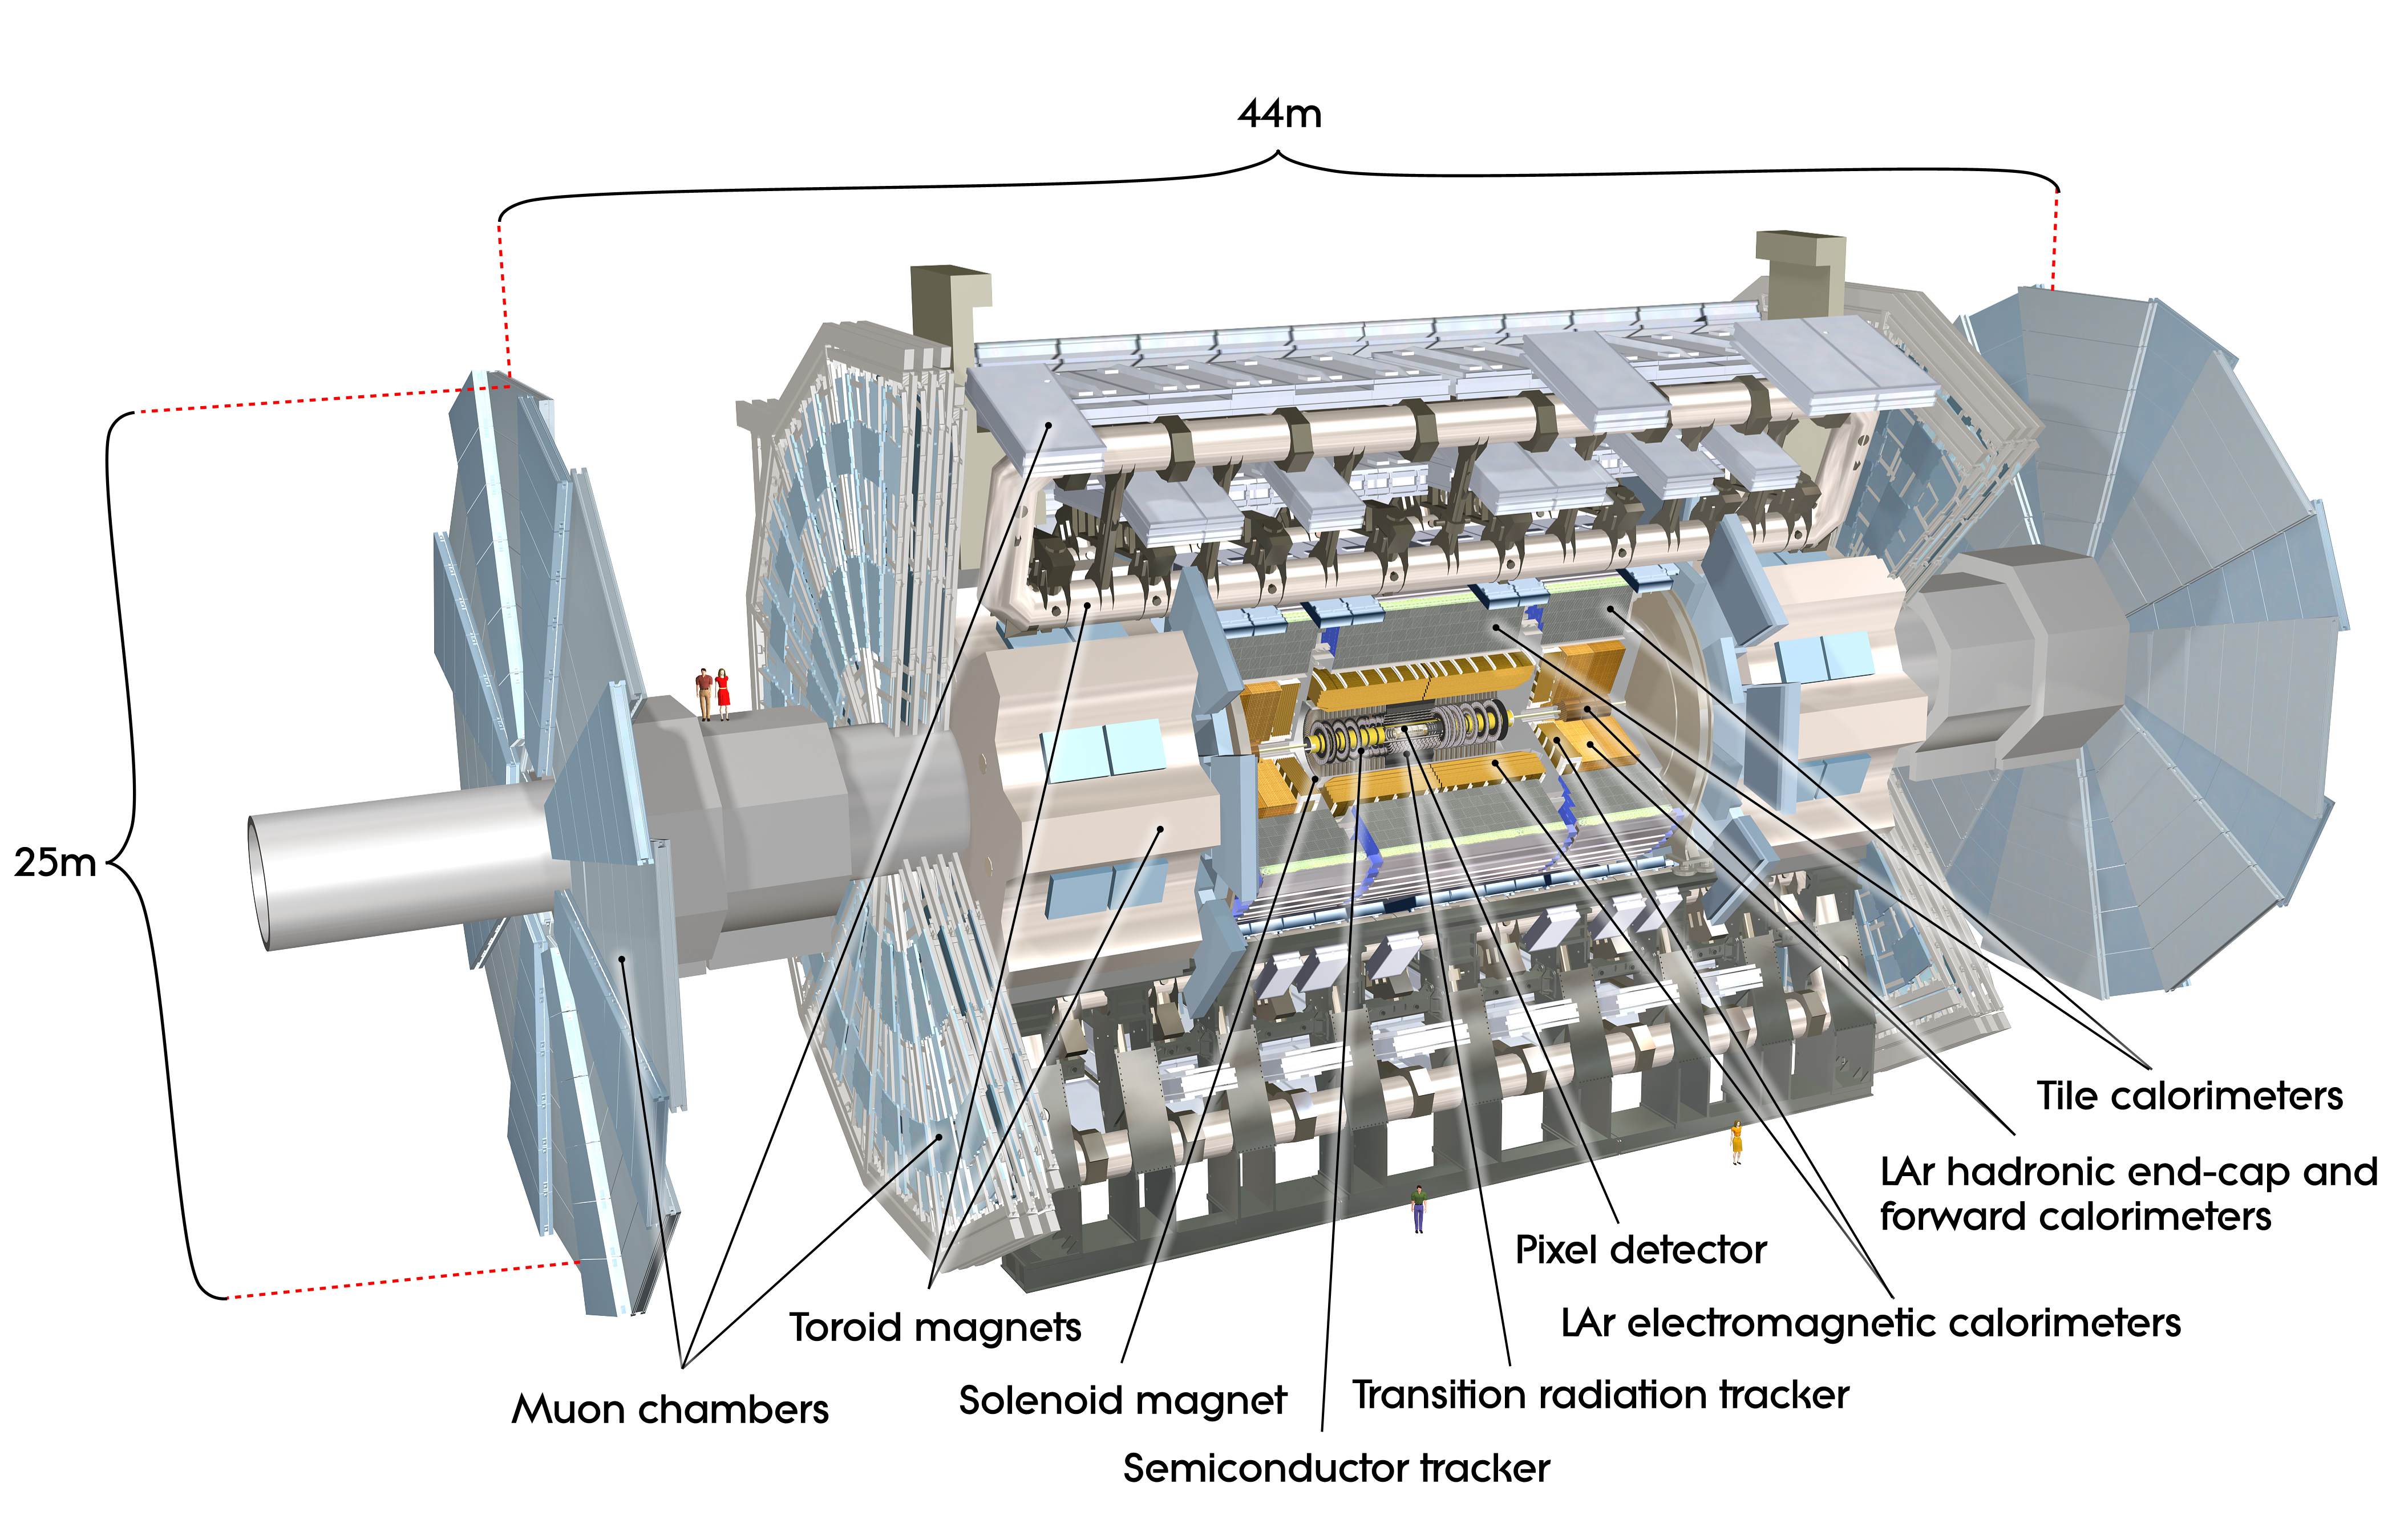
\includegraphics[width=0.75\textwidth]{figures/chapter_ATLAS/ATLASDetector}
        \caption{
			Computer generated image of the ATLAS detector\cite{Pequenao:1095924}. Showing the different parts of the components involved. 
        }
        \label{fig:ATLASDectector}
    \end{center}
\end{figure}


\subsection*{The ATLAS coordinate system}

The ATLAS detector uses a cylindrical coordinate system: Z-$\phi$-$\eta$ to describe the particles location after interactions.
The z-axis runs along the beamline and starts at the origin (center and middle) of the detector. The x-y plane perpendicular to the z-axis described as the transverse plane is represented in the polar coordinate~\ref{fig:Coordinates}. The plane is described by two angles: $\phi$ is the 2$\pi$ azimuthal angle on the x-y plane and the 1$\pi$ polar $\theta$ angle with respect to the z axis is given in term of psuedorapidity, the term is Lorentz invariant and is its conversion to theta is given
by Eq.~\ref{eq:Eta}. The $\delta R$ quantity is used to describe the angular distance between particles, it's defined in Eq.~\ref{eq:deltaR} This quantity is approximately Lorentz invariant. Figure~\ref{fig:Coordinates} shows the ATLAS coordinate system. Figure~\ref{fig:pseudorapidity} shows the pseudorapidity($\eta$) to angle conversion. 

\begin{equation}
    \eta=ln(tan(\theta/2))
    \label{eq:Eta}
\end{equation}

\begin{equation}
\delta R=\sqrt{\delta\eta^{2}+\delta\phi^{2}} 
\label{eq:deltaR}
\end{equation}

\begin{figure}[!htb]
    \begin{center}
        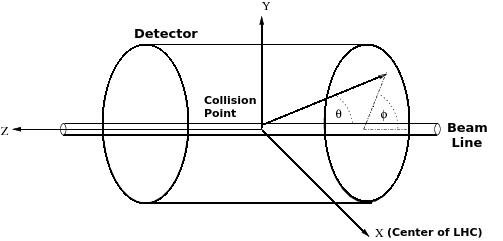
\includegraphics[width=0.75\textwidth]{figures/chapter_ATLAS/Coordinates}
        \caption{
            This figure displays the coordinate of the ATLAS detector system~\cite{2008}.
        }
        \label{fig:Coordinates}
    \end{center}
\end{figure}

\begin{figure}[!htb]
    \begin{center}
        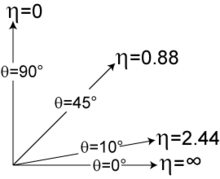
\includegraphics[width=0.75\textwidth]{figures/chapter_ATLAS/pseudorapidity}
        \caption{
            Pseudo-rapidity $\eta$ to angle in degree conversion~\cite{enwiki:1052183914}.
        }
        \label{fig:pseudorapidity}
    \end{center}
\end{figure}



\subsection{Inner Detector}
The inner detector(ID) is the innermost part of the ATLAS detector. Its main function is to record charged particle trajectories. The tracks provide valuable information for the reconstruction of the primary vertices of particle interactions. All four parts of the ID are enclosed by a superconducting solenoid magnet of 2T aligned along the beamline, charged particles are curved into helical trajectories along the beamline. This is be used for charge, mass and momentum calculation as well as particle
identification. 

% TODO insert charge to mass trajectory calculation


The inner detector is made up of four different parts. From inside out, the Insertable B Layer, the Pixel detector, the Semi-Conductor Tracker(SCT) and the Transition Radiation Tracker(TRT). 
Its resolution is the highest in the innermost part of the detector and decreases outward. The following is a detailed description of the four parts of their coverage and detector mechanism. 

Closest to the core of the detector is a very high-resolution insertable B layer(IBL). It was inserted after Run I to further extend the pixel detector coverage to $|\eta|< 2.9$. This helps with b-hadron identification through better vertex reconstruction.

Around the IBL is the Pixel detector. It is made of three layers of fine silicon pixels of spatial resolution of 10$\mu$ m in the r-$\phi$ direction and 115$\mu$ m in the z-direction. It provides a cylindrical coverage that covers up to $|eta|<2.5$. Electron-hole pairs are generated when charged particle passes through the silicon pixel which the signal is then read out through the applied electric field.
Surrounding the pixel detector, there is a silicon microstrip detector called the Semi-Conductor Tracker (SCT), located in radii between 30-51 cm, which is made up of 4 layers of strip silicon sensor. Each SCT layer is made up of two overlapping sets of silicon strips at an angle with one another. The working mechanism of the detector is similar to that of the pixel detector, but the resolution is slightly reduced to 17 $\mu$m in the r-$\phi$ plane and 580 $\mu$ m along the z-axis. 
The outermost part of the ID is called the Transition Radiation Tracker(TRT), made up of gas-filled straws. There are 70 layers in the barrel and 140 layers in each end cap covering up to $|\eta|<2.0$. Each straw tube contains gas that can be ionized by charged particles, the electron formed in the process will then move toward the charged center of the straw to be read out for momentum, trajectory and charge calculation. The TRT also helps with particle identification, as charged particles alsoemit a photon and this probability is related to the Lorentz factor. Lower mass electrons emit more photons than charged hadrons. Therefore, this can be used to identify electrons over hadrons on top of track reconstruction. The TRT has a resolution of 130$\mu$ m in the r-$\phi$ plane.

\begin{figure}[!htb]
    \begin{center}
        \includegraphics[width=0.4\textwidth]{figures/chapter_ATLAS/InnerDetector1}
        \caption{
            This image shows the computer generated image of the inner detector~\cite{Pequenao:1095926}.
        }
        \label{fig:InnerDetector}
    \end{center}
\end{figure}

\begin{figure}[!htb]
    \begin{center}
        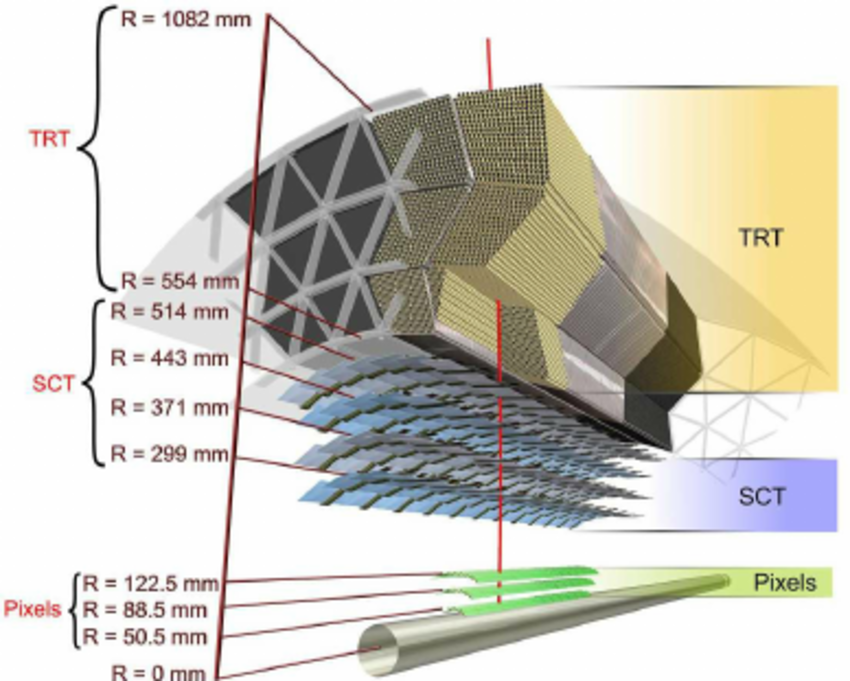
\includegraphics[width=0.75\textwidth]{figures/chapter_ATLAS/InnerDetector2}
        \caption{
            This image shows the computer generated image of the inner detector and its inner layout~\cite{Pequenao:1095926}.
        }
        \label{fig:InnerDetector2}
    \end{center}
\end{figure}

\subsection{Calorimeter}
The main function of the calorimeter is to provide energy measurement for particles. The ATLAS Calorimeter is split into two parts, sorted by the particle interaction method, The Electromagnetic-Calorimeter(E-Cal) utilizes the electromagnetic interaction and measures energy deposit in the form of electron and photon showers; the Hadronic Calorimeter uses strong hadronic interactions, energy is measured in the form of a hadronic shower in quarks and gluons. Both systems utilize a dense passive material for the particle showering and are sampled through a layer of sensitive active element for detection. Below, different components of the ECAL and the HCAL will be described in detail. 

After tracking, the particle will first reach the ECAL. The first layer is the liquid-argon(LAr) electromagnetic(EM) calorimeter. The passive medium for showering is lead. The endcap portion covers $1.375< |\eta| < 3.2$, and the barrel cover up to $|\eta|<1.475$. The innermost layer has the greatest granularity of 0.003, the second layer has a resolution of 0.025 and the third layer is the most coarse. 

The hadronic calorimeter(HCAL) measures hadron showering in the form of quarks and gluons, the barrel portion is made of a tile calorimeter, it uses steel as the passive element for showering and scintillating tiles as the readout active element and the 

The forward calorimeter end cap uses LAr for both the ECAL and HCAL, but copper-tungsten is used as the passive layer instead. 


\begin{figure}[!htb]
    \begin{center}
        \includegraphics[width=0.75\textwidth]{figures/chapter_ATLAS/Calorimeter}
        \caption{
            This image shows the computer generated image of the calorimeter and its inner layout~\cite{Pequenao:1095927}.
        }
        \label{fig:Calorimeter}
    \end{center}
\end{figure}

\subsection{Muon Spectrometers}
The muon spectrometer(MS) measures both the trajectory of muons and perform their triggering. The only type of particles that make it past the calorimeters and reach the muon spectrometer are either non-interacting particles, or they are the minimum ionizing particles, muons. Tracking and measurement of muons can effectively distinguish them from the non-interacting particle which could be neutrinos or beyond the standard model physics particles like dark matter. 
The muon spectrometer system of ATLAS is surrounded by the superconducting toroid magnets, the barrel toroid provide up to 0.5 T between $1.6 < |\eta|<2.7$ , the end cap toroids provide up to 1T. The magnet bends the particles along the beamline into the end caps.
For precision tracking, the muon system is made up of the Monitored Drift Tubes(MDTs) in both the barrel and the endcap region, in the forward region there is a Cathode Strip Chamber(CSCs) in region $|\eta|>2.7$
For triggering, it uses the Resistive Plate Chamber(RPC) in the barrel and the Thin Gap Chambers (TGCs) in the end cap for fast readout. 

%Comparison with CMS

\begin{figure}[!htb]
    \begin{center}
        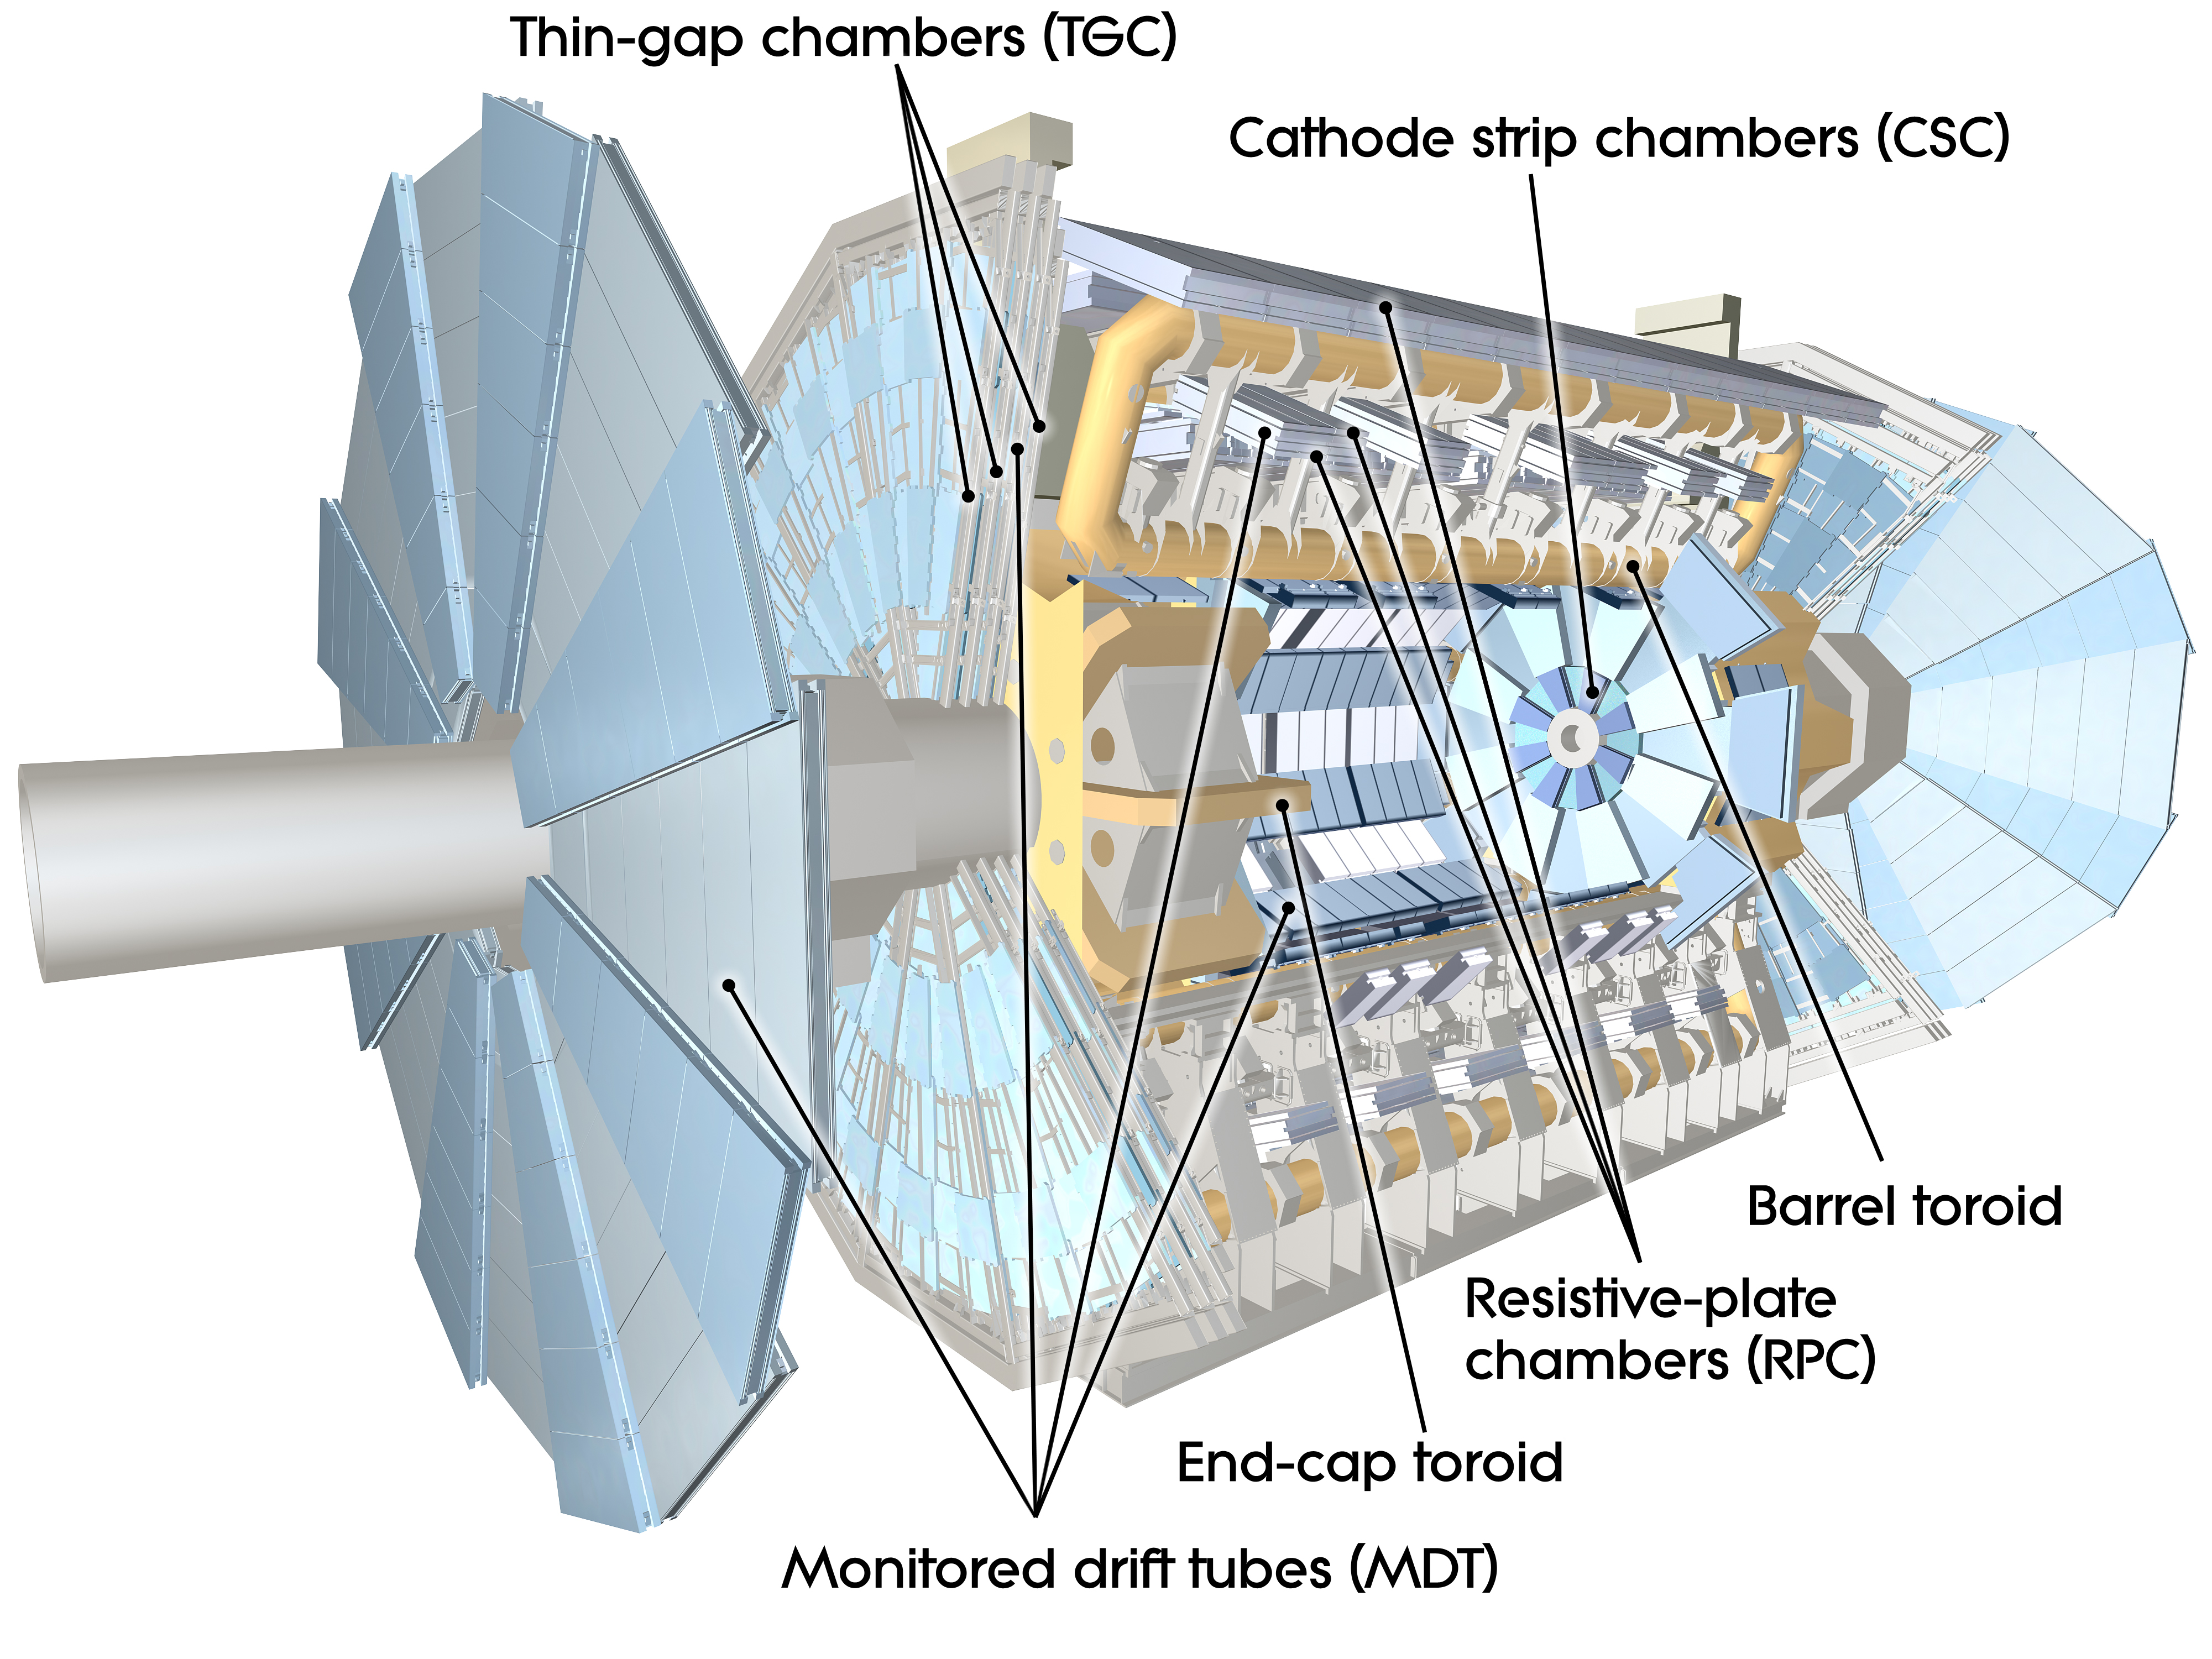
\includegraphics[width=0.75\textwidth]{figures/chapter_ATLAS/MuonSpectrometer}
        \caption{
            This image shows a computer generated image of the muon spectrometer~\cite{Pequenao:1095929}.
        }
        \label{fig:MuonSpectrometer}
    \end{center}
\end{figure}

\section{Data Acquisition of ATLAS}
\label{trigger}
%Data acquisition of ATLAS 
During Run II, the LHC performed proton-proton collision at $\sqrt{s}=13 TeV$ at the instantaneous luminosity of $10^{34}cm^{-2}s^{-1}$. An approximate of 33.7 pp interaction per bunch crossing was delivered. 
At this collision rate, not all data could be processed and saved. The process of selecting experimentally interesting events is called ``triggering". In Run II, triggering is administered and controlled by a central trigger processor which assigns different information from detectors to different part of the trigger computing system. There are two levels of triggering in ATLAS Run II, the low level hardware-based trigger is called L1 triggers, the second level software based high level triggering is called the High-level trigger(HLT). 
The L1 trigger filters through the input at 40 MHz to 100kHz. This is done by looking at energy deposits at the calorimeters that could be
candidate leptons, jets, or photons. Muons are triggered by the hits that formed towers in the MS system. 
Events that pass through the L1 trigger will then be passed onto the HLT. The HLT further filters the 100kHz events received to 1kHz for writing to disk for offline analysis. The HLT is software-based it further defines region-of-interest in detector and filter events that do not fit the trigger selection criteria. High-level objects are created from
the online information and an event loop is used to discard events that do not fulfill the trigger criteria.
Events are saved to ``trigger chains" for later analyses, they are sorted into different analysis derivations with basic criteria applied for different types of analyses. 

\begin{figure}[!htb]
    \begin{center}
        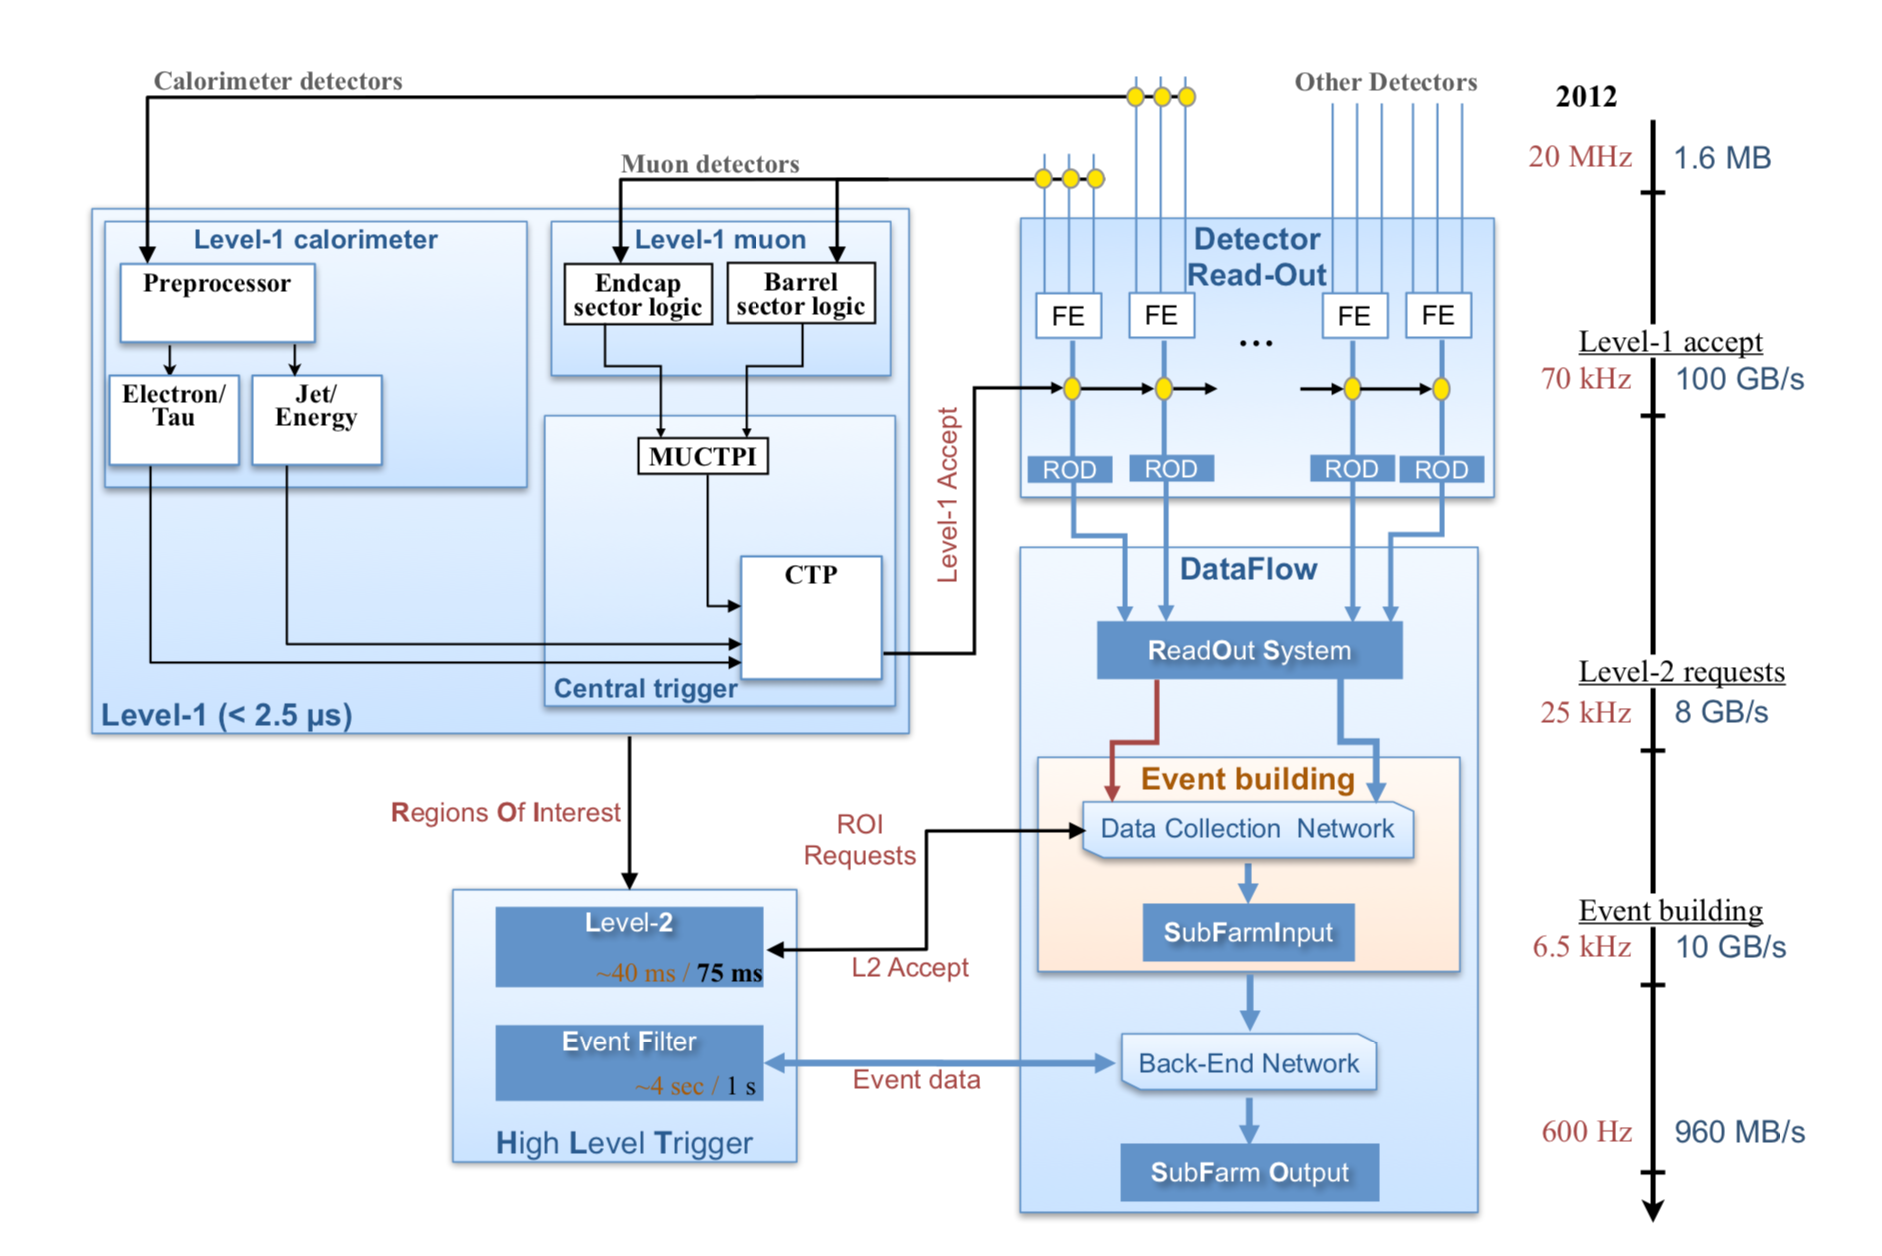
\includegraphics[width=0.75\textwidth]{figures/chapter_ATLAS/TDAQ}
        \caption{
            This image shows the schematic overview of the ATLAS triggering system~\cite{Pequenao:1095929}.
        }
        \label{fig:TDAQ}
    \end{center}
\end{figure}


%\chapter{the New Small Wheel Upgrade}
\label{chapter:NSW}

\chapter{Common Analysis Items}
\label{chapter:CommonAnalysisItems}

%todo IO muons
%todo
After collisions in the LHC, the particles hits exist as different electronic signals from various detector components saved in hard disk, converting these signals into physics objects worth analyzing takes different reconstruction, identification, cleaning, and calibration steps. This chapter will discuss the different steps these detector hits go through before they become analysis-ready physics objects. 

\begin{figure}[!htb]
    \begin{center}
        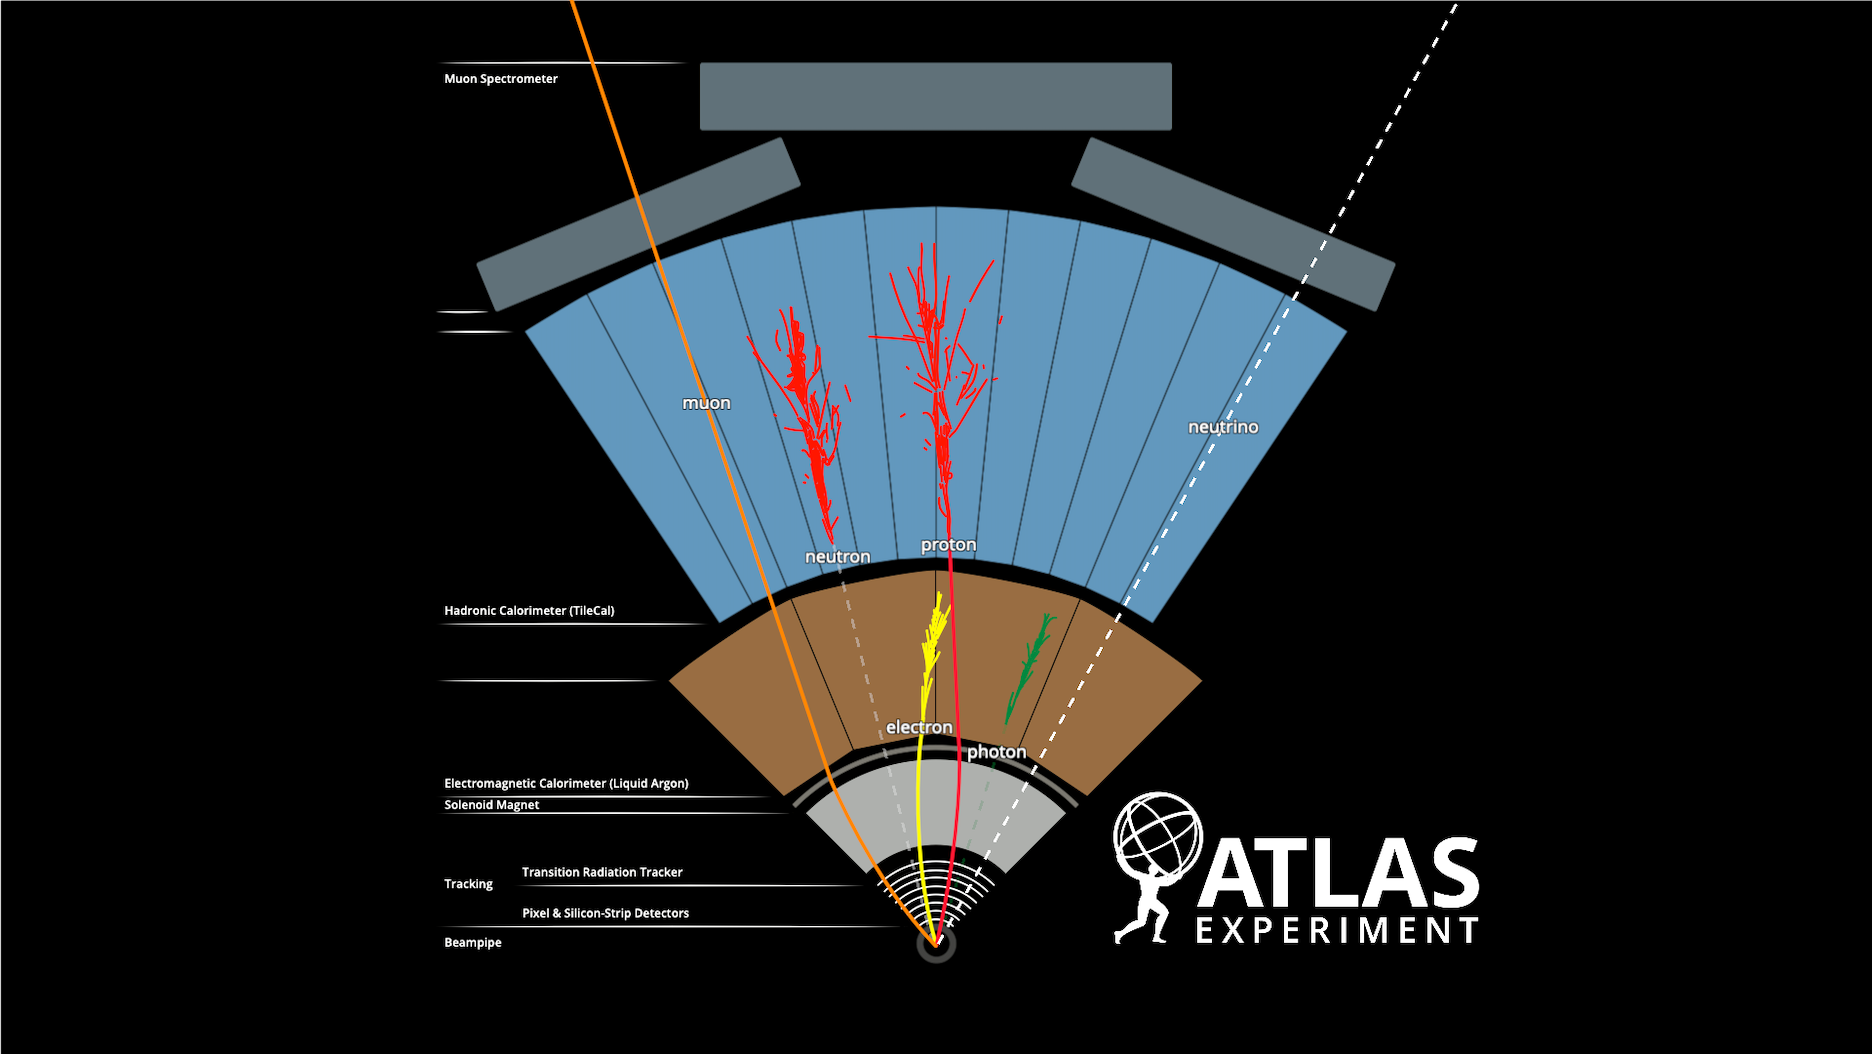
\includegraphics[width=1.1\textwidth]{figures/common_ana/ParticleSignature}
        \caption{        
            Different particles displays a different particle signature characteristics in the ATLAS detector\cite{Mehlhase:2770815}.
        }
        \label{fig:isolationWP}
    \end{center}
\end{figure}

\section{Tracks and primary vertices}

Charged particles leave trajectories in two distinct ATLAS sub-detector systems, namely the inner detector(ID) and the muon system(MS). The inner detector is made up of the pixel detector, the Semiconductor Tracker, and the Transition Radiation Tracker(TRT). Tracking is done for all particles that are charged. 
The MS is made up of Monitored Drift Tubes(MDTs), the Cathode Strip Chambers(CSC), Thin Gap Chambers(TGC), and the Resistive Plate Chambers(RPC). It's mainly used for
track formation of muons, which are minimizing particles that through all of the ID and calorimeters.


\subsection*{Tracks}
To reconstruct a hit from detector raw hit information, a couple of  coincidence measurement across the different subsystems will be used to form a track seed. Then, a Kalman filter is used to fit the tracks,  irrelevant hits from pile-up are removed through the filter rejection.  
A track formed this way is described by the following few track-associated parameters: ($d_{0}$, $z_{0}$, $\phi$, $\theta$, q/p).
%by forward filtering, backward smoothing and outlier rejection of

\begin{figure}[!htb]
    \begin{center}
        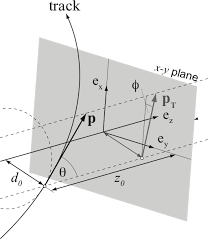
\includegraphics[width=0.45\textwidth]{figures/common_ana/Track}
        \caption{ 
            Track reconstruction in ATLAS. Schematic view of how the parameters associated with track creation.
        }
        \label{fig:isolationWP}
    \end{center}
\end{figure}


\subsection*{Primary Vertex}
Once tracks are formed in the inner detector, primary vertices can be constructed to discriminate an event from other hits. 
Primary vertices are the initial interaction point where the further decay particles that reach the ATLAS detector are formed. Verticing is important as it is effective in discriminating pile-up hits from the ones from the event-of-interest. This is increasingly important in newer LHC runs where the higher luminosity has resulted in additional in-time and out-of-time pile-ups. 

\begin{figure}[!htb]
    \begin{center}
        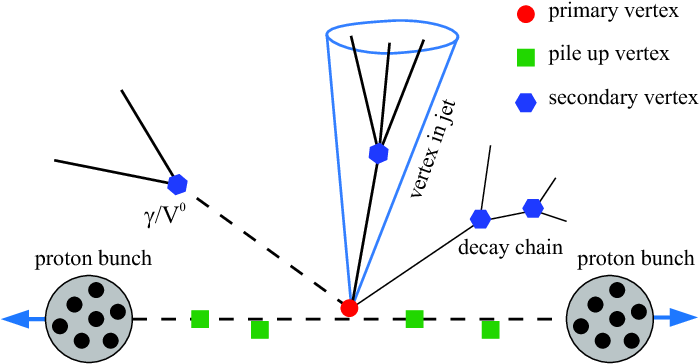
\includegraphics[width=0.75\textwidth]{figures/common_ana/Vertex}
        \caption{        
            Schematic view showing vertexing in ATLAS\cite{4774734}.
        }
    \end{center}
\end{figure}
Vertexing is consist of a couple of different steps:

1. A vertex seed is found by filtering the point where most interactions are found. This is done by an iterative method or imaging method.  

2. Tracks consistent with the chosen vertex seed are put into a group.

3. An adaptive vertex fitting algorithm is used to find the position and the associated error of the vertex. 

4. The unused tracks are used for the next vertex creation. 

There are usually a couple of primary vertices in each bunch crossing, the vertex with the highest PT particles originated from it is considered the hard-primary vertex of the event, the others are considered the pile-up primary vertices. 

With tracks and primary vertices constructed, particle reconstruction can begin. 


\section{Muons}
Muons on ATLAS formed from the tracking and primary vertex information from both the ID and the MS described in the above section. Additinoal information from the calorimeter is also used. There are four main muon reconstruction strategies. Mainly due to different PT muon in different detector location will require different strategies for optimal reconstruction efficiency. There are four muon working points, which uses different reconstruction strategy combination and discriminating cuts to
increase the identification efficiency for different analyses.

\begin{figure}[!htb]
    \begin{center}
        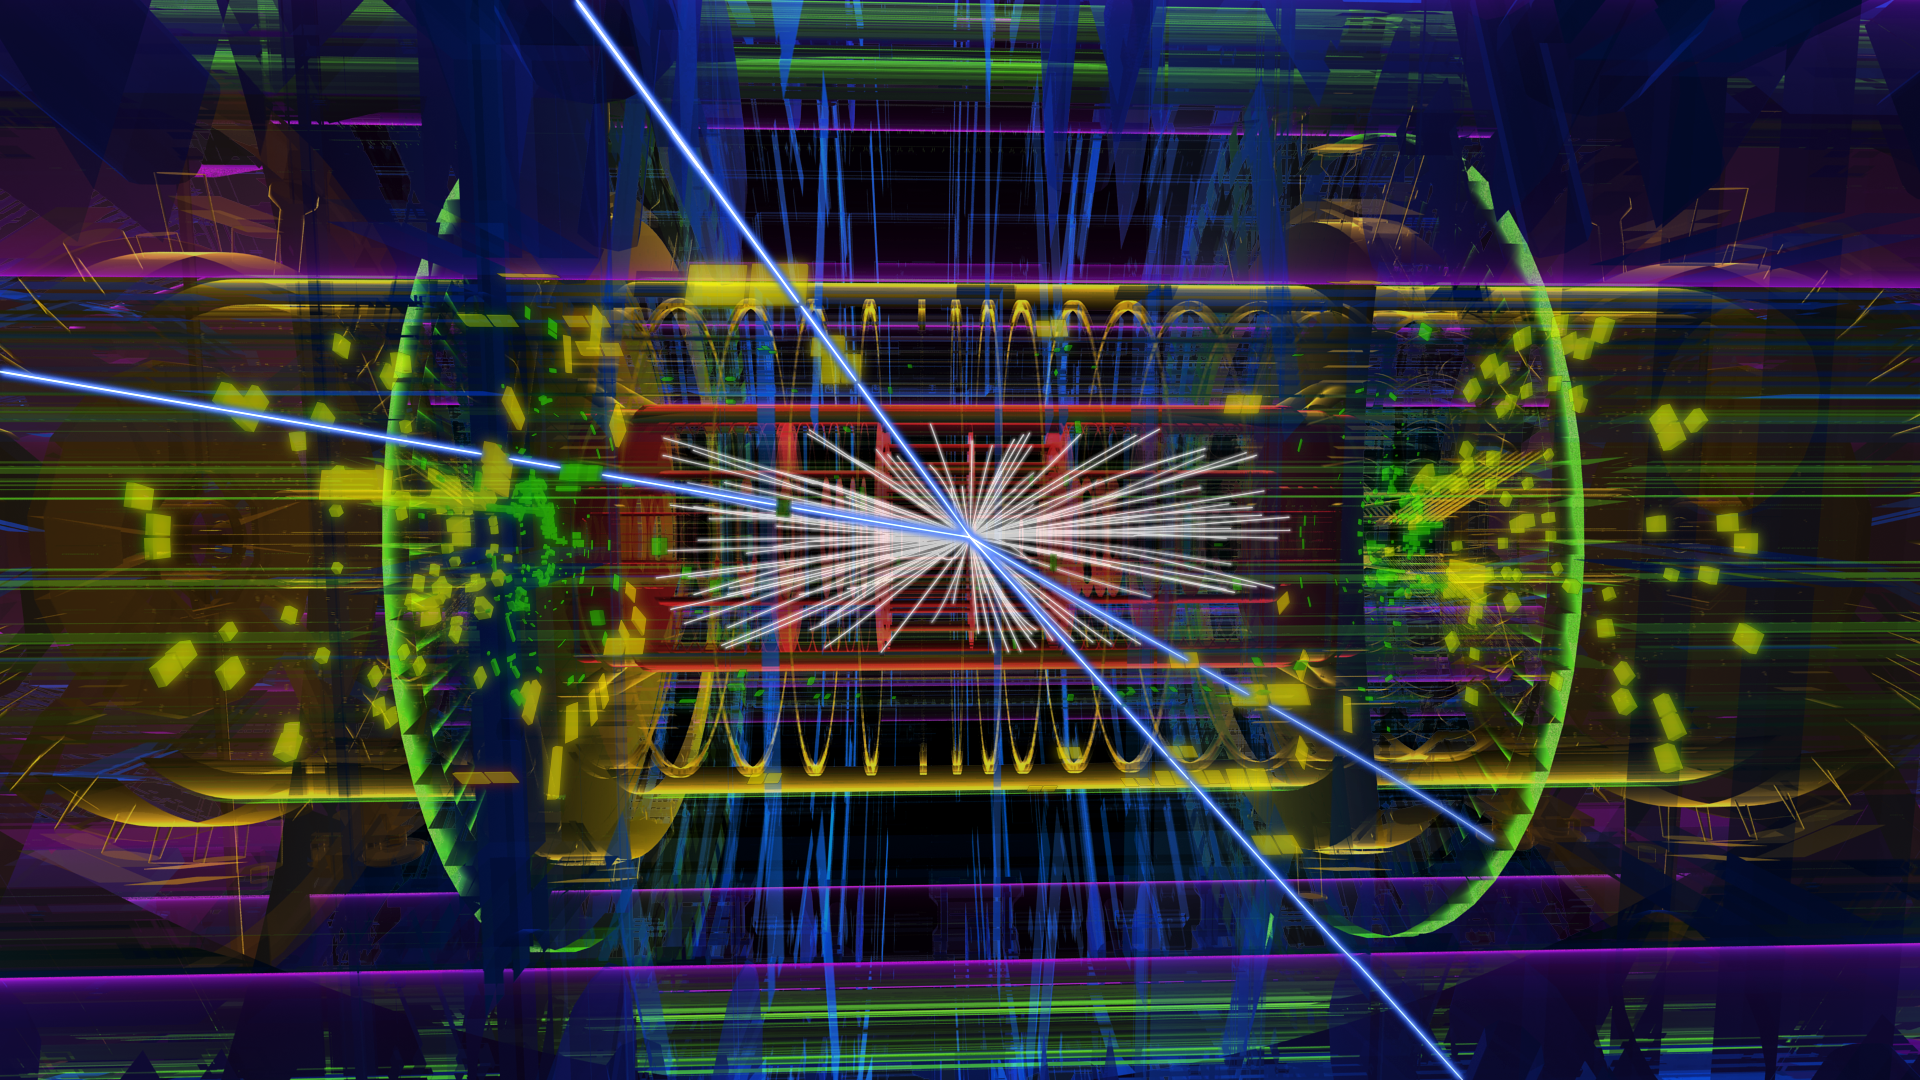
\includegraphics[width=0.85\textwidth]{figures/common_ana/Muon}
        \caption{        
            Event visualization of a four muon event in the ATLAS detector\cite{ATLAS:1697053}.
        }
    \end{center}
\end{figure}

These strategies and working points are result from studies done on the standard samples of Z to $\mu \mu $ and $J/\Psi$ to \mu \mu. 
%As different muon transverse momentum will lead to muon hits depositing in different parts of the detector and different region also require different strategy for best differentiation. 
%forward region also present more difficult muon finding conditions, given this four different muon algorithms are developed. 

\subsection{Muon Reconstruction}
A similar principle is utilized for all four strategies: tracks are found in one part of the detector through pattern finding from hit patterns in the chambers. At least two matching segments from different subdetector parts is needed to form a track candidate. From the track candidate, a couple of global $\chi^{2}$ fits is done to associate other hits and drop outlier from the fit, while removing the outlier hits. The main goal of muon reconstruction is to increase the
reconstruction efficiency, which is the ratio between muon reconstructed and the number of truth muons. 

\begin{itemize}
\item Combined (CB) muon
This strategy is optimal for the muons that are detected in both the ID and the MS in both the barrel region and end-cap region of the detector. Tracks are each constructed from the ID and the MS and a global refit done to remove outliers to improve the fit quality. This is mostly done by an outside-in approach where the tracks in MS are made to match the ones seen in the ID. 

\item Inside-out(IO) muons
    This strategy complements the Combined muon approach and finds muons from an inside-out algorithm. It looks for MS hits that can be associated with ID tracks and recovers some muons that don't make it to the MS fully. 

\item Segment-tagged (ST) muons
This method is used to identify lower PT muons that couldn't make it to multiple layer of the MS. If a track in the ID can be matched to at least one track segment in the MDT in the barrel or CSC in the end-cap, it will be selected as a segment-tagged muon. 

\item Calorimeter-tagged(CT) muon
This method is for even lower PT muons that could not make it to the MS at all. Muons between 15 < $P_{T}$ < 100GeV is formed from matching a track in ID with energy deposit in the calorimeter that matches the minimum-ionizing particle. This is optimized for barrel muons of $|\eta <0.1|$. 

\item Extrapolated(ME) muon}
This strategy is for muons that are very forward and is swamp under noise from pile-up. Muon tracks in the MS chamber with a loose compatibility to the originating IP are ME muons are accepted as ME muons. This strategy extending the acceptance of muons in the forward region from 2.5< $|\eta|$<2.7, where there is no ID coverage and cannot be reconstructed by the above other methods.

\end{itemize}

\subsection{Muon Identification}
Muon identification is a set of selection criteria done on the candidate muons to cut out background from pions/kaon decays that would form muons that are not of interest to analysis. This increases the analysis signal sensitivity. In different analyses, depending on the signal type, different muon identification working points are used.

A couple of criteria are used for muon identification: $q/p_{significance}$, $\rho'$ and $\chi^{2}_{norm}$. They are defined as below:

\subsubsection*{Discrimination Criteria}
\begin{itemize}

\item q/p significance
    \begin{equation}
    $$ q/p_{significance} = |(q/p)^{ID} - (q/p)^{MS}|/\sqrt{\sigma^{MS}_{PT} + \sigma^{ID}_{PT}} $$
    \end{equation}

This is the absolute value of the difference between the charges and the PT measurement divided by the sum of error in the PT measurement of both the ID and MS.

\item $\rho'$
    \begin{equation}
    $$ \rho' = |P_{T}^{MS} - P_{T}^{ID}| / P_{T}^{Combined} $$
    \end{equation}

This is the absolute value of the difference between the PT of the MS and the ID divided by the combined PT of the muon candidate.

\item $\chi_{norm}^{2}$

    This is the $chi^{2}$ of the fit from the combined muon track from both the ID and MS.

\end{itemize}

These selection criteria for the muon groups above result in five different working points.


\subsubsection*{Muon Working Points}
\begin{itemize}

\item MEDIUM \newline
This is the most commonly used working point. q/p significance $<$ 7. It accepts only the CB and IO muons.  

\item LOOSE \newline
    The loose working point accepts all the muons that pass the medium working point. It also accepts low-PT muons, including IO muons with PT lower than 7GeV. Some ST and CT muons are also accepted if they pass certain requirements. 

\item TIGHT \newline
    This working point accepts a subset of the medium working point muons. In addition, they are required to have a normalized $\chi^{2}$ of less than 8. The requirement on q/p compatibility and $\rho'$ depends on $\eta$ and $P_{T}$ of the muon.

\item HIGH $P_{T}$ \newline
This working point only accept muons that also pass the medium working point requirement. Owing to their high PT, the reconstruction can be done with the MS alone for a higher resolution.


\item LOW $P_{T}$ \newline
The Low-$p_{T}$ working point includes all of the muons in the medium working point, it's identical to the medium working point muon set above $P_{T}=18GeV$. But this working point also includes muons with lower pt that does not make it to the middle of the MS, this working point includes muons down to 3 GeV. 

\end{itemize}

\begin{figure}[!htb]
    \begin{center}
        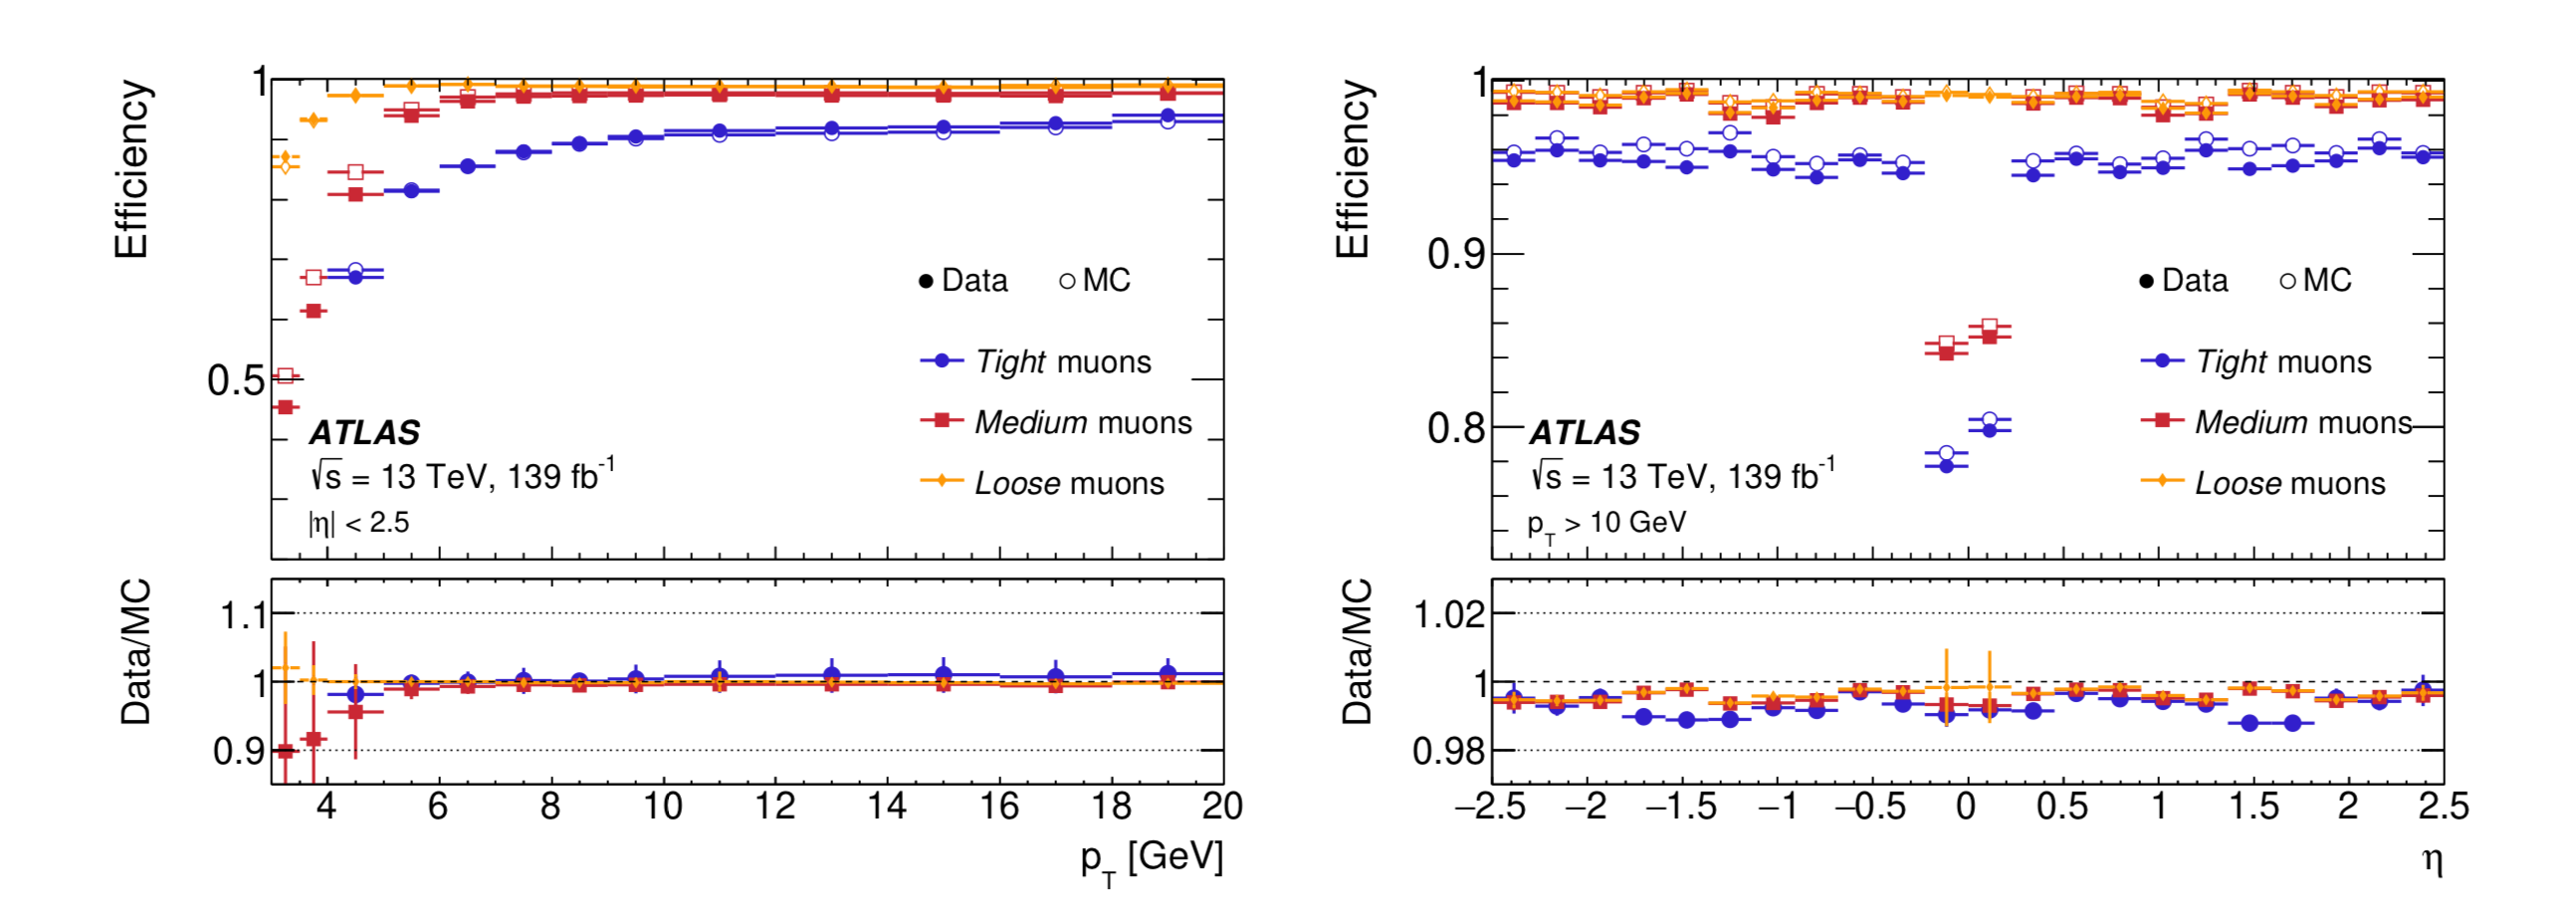
\includegraphics[width=1\textwidth]{figures/common_ana/IdentificationEff}
        \caption{
            This figure shows the reconstruction and identification efficiencies in different variable range in different working points\cite{Aad:2746302}.
    }
        \label{fig:isolationWP}
    \end{center}
\end{figure}



\subsection{Muon Isolation}
In addition to the reconstruction and identification working point, muon isolation is to pick out the muon candidates of interest and drop other ones to the analysis for better sensitivity. On ATLAS, the interesting leptons came from the hard primary vertex decay of radially decaying particles. W, Z, Higgs bosons or other BSM particles such as the Z' are examples decays that concern analyzers. Muons formed are known as "prompt muons", usually clean and do not have many associated neighboring hits. Less interested muons came from the semileptonic decay from jet fragmentation, these muons decays are formed with lots of
neighboring hits. The neighboring hits can be used as criteria to discriminate interesting muons from the less interesting ones, the step is called muon isolation. This increases the signal sensitivity by cutting down the background in searches and measurements.
%They are often classified as "background" processes. To distinguish these leptons and increase signal significance for the lepton
%from processes that concerns us, an isolation criteria is used. 
There are two variables used for muon isolation, one is track-based isolation and the other is calorimeter-based isolation. 

\subsubsection*{Isolation Parameters}
The parameters used in the isolation criteria are defined as the following:
\begin{itemize}
    \item  $P_{T}^{varcone\:size}$ \newline
        The track-based isolation variable, $P_{T}^{varcone\:size}$ are the sum of the PT of all the tracks in a variable-sized cone. The variable-sized cone(varcone) is defined as below.

    
\[ \delta R = min(\frac{10}{P^{\mu}_{T}[GeV]}, \delta R_{max}) \]
The term is PT dependent, the larger the PT, the smaller the cone. 
    \item $E^{topocone\:size}_{T}$ \newline

        A calorimeter based parameter $E^{topocone\:size}_T$ is defined as the sum of the energy deposit in a $\delta R$ size topo cone. 

\end{itemize}

The isolation criteria using the track-based variable is the isolation variable to the transverse momentum to the muon. Studies are done on data Monte Carlo to get the best cut-off point. The different working points are listed as below~\ref{fig:isolationWP}.

%\section{Muon scale and resolution}

\begin{figure}[!htb]
    \begin{center}
        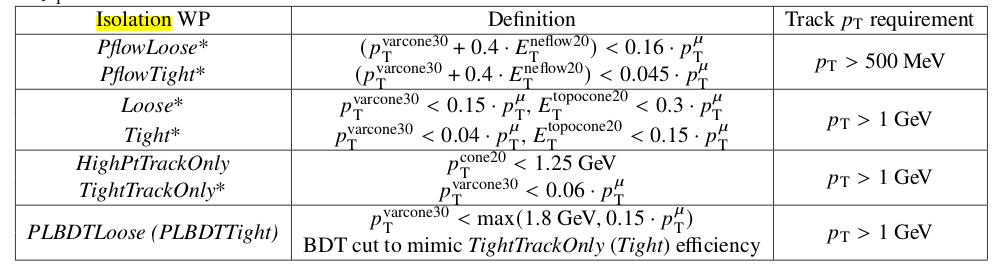
\includegraphics[width=0.75\textwidth]{figures/common_ana/Isolation}
        \caption 
        {
            This figure shows the isolation working points on ATLAS from full run2\cite{Aad:2746302}.}
        \label{fig:isolationWP}
    \end{center}
\end{figure}

\begin{figure}[!htb]
    \begin{center}
        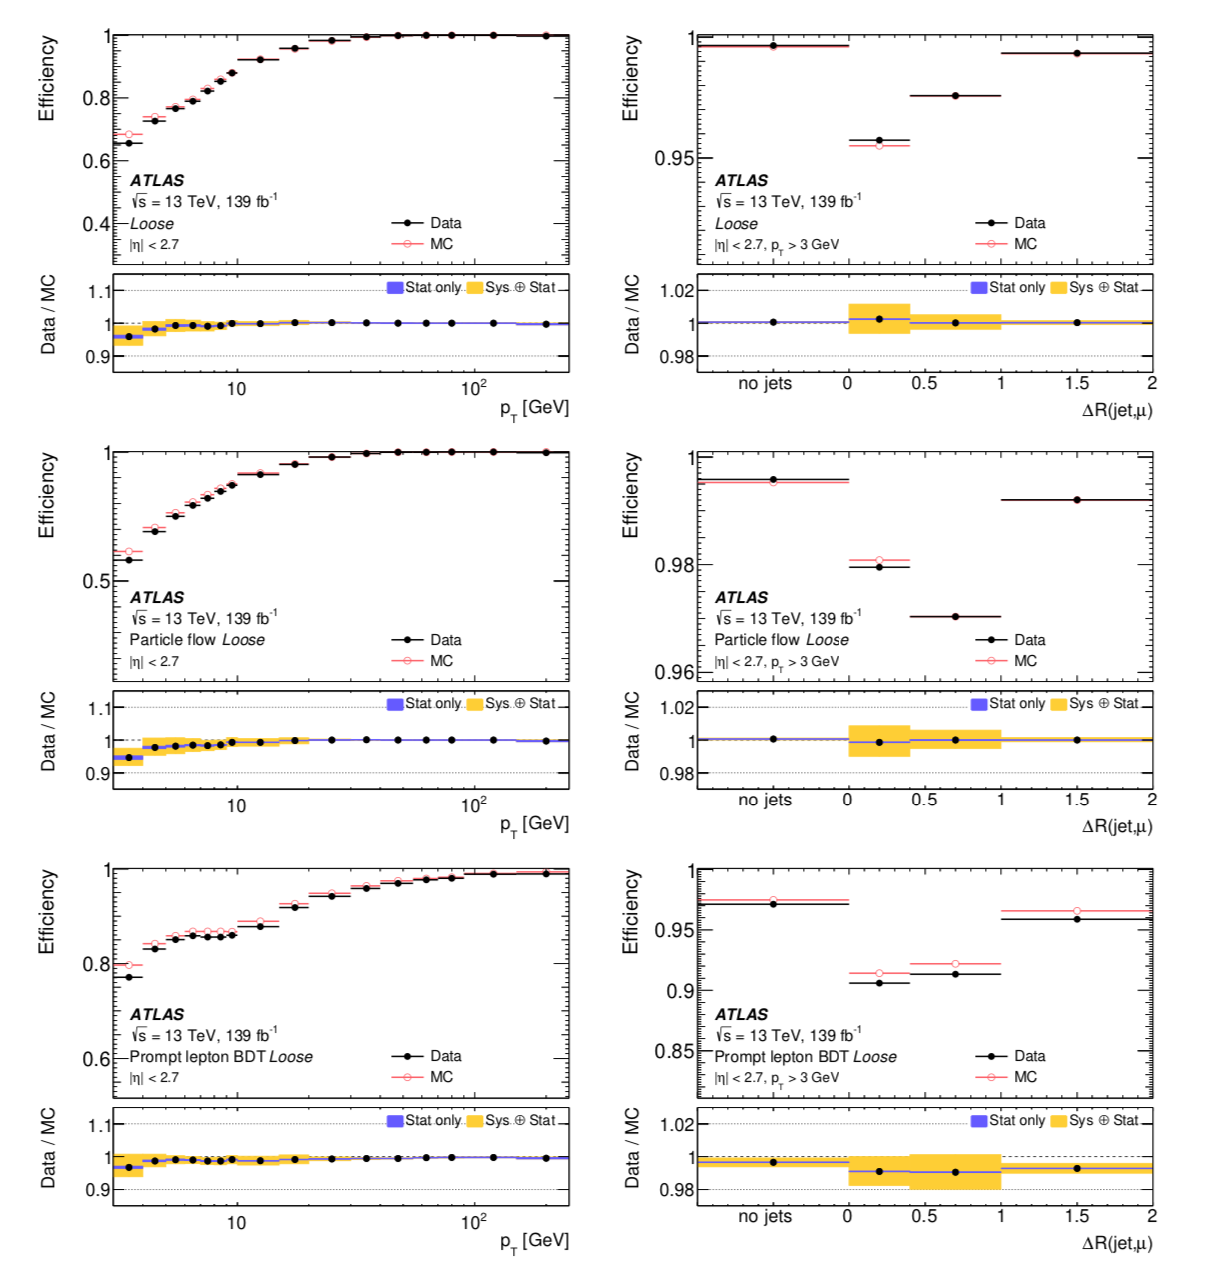
\includegraphics[width=0.75\textwidth]{figures/common_ana/IsolationEff1}
        %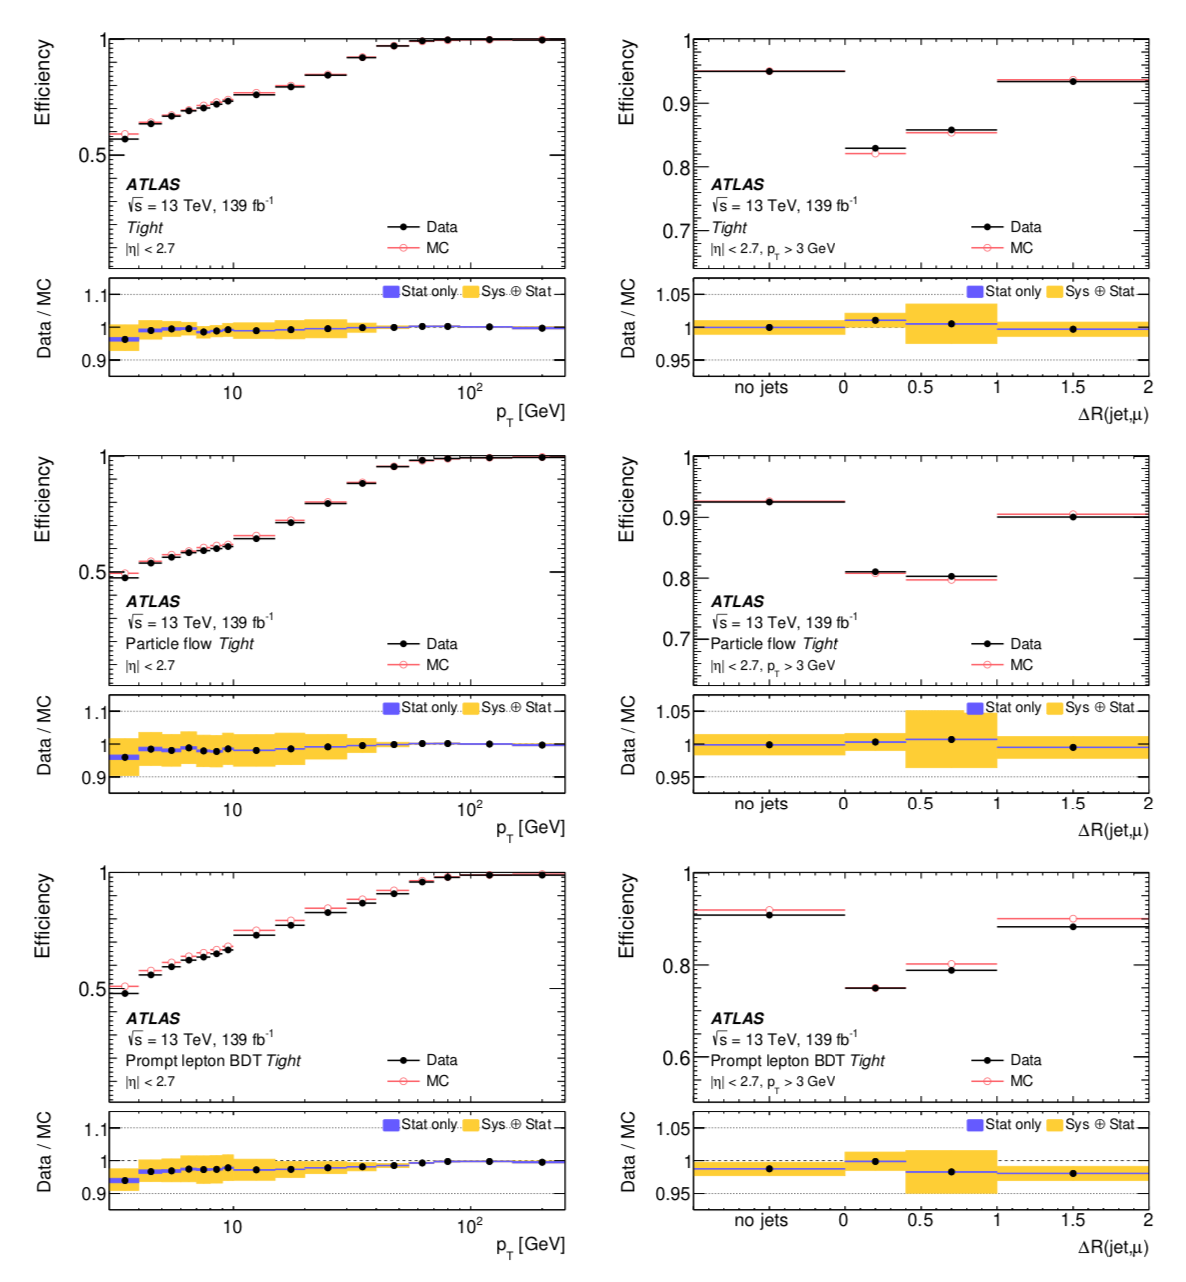
\includegraphics[width=0.75\textwidth]{figures/common_ana/IsolationEff2}
        \caption{
            This figure shows the isolation efficiency in different variable range in different working point\cite{Aad:2746302}.
        }
        \label{fig:isolationWP}
    \end{center}
\end{figure}


\subsection{Muon Calibration}
Given the difference between imperfect Monte Carlo generation and data, a calibration factor is derived from comparing the MC to data for some known physics process $J/\Psi$ to $\mu \mu$ and Z to $\mu \mu$. The calibration is done on the PT of the muon. 
The calibration is dependent on the detector angle, and the formula is summarized as below, where the constants are derived from the data and simulation of the samples.

%In data there is always margin for calibration error, and monte carlo is also not necessarily accurately describing the experimental environment. To match data result to the actual physics process that happened, transverse momentum correction done on both the MS tracks muons and the ID track on the MC result as follows: 

\begin{equation}

\[ P_{T}^{Cor,Det} = \frac{P^{MC, Det}_{T} + \sum_{n=0}^{1} S_{n}^{Det}{\eta, \phi}(P_{T}^{MC, Det})^n}{1+\sum_{m=0}^{2}\delta r_{m}^{Det}(\eta, \phi)(P_{T}^{MC, Det})^(m-1) g_{m}} \]
\label{eq:muoncalib}
\end{equation}


where $P_{T}^{MC, Det}$ is the uncorrected transverse momentum, $g_m$ is a unit Gausssian distribution, $\delta r^{Det}_{m}(\eta, \phi)$ and $s_{n}^{Det}(\eta, \phi)$ are the momentum resolution smearing and scale correction resolution. 

The correction is then applied to the combined muon in the following way:

\begin{equation}
\[ P_{T}^{Cor, CB} = f *P_{T}^{Cor, ID}+ (1-f) \cdot p_{T}^{Cor, MS}\]
\label{eq:muoncalibfactor}
\end{equation}

The weight f in the above is obtained from MC simulation. 



%\begin{equation}
%\[\delta R = min( \frac{10}/P_{T}[GeV] , \delta R_{max} )\]
%\end{equation}



%For better discrimination effciency, in Run II, ATLAS has moved away from an iterative based method and moved towards a image algorithm for primary vertex finding. A brief description is as the
%following:  
%
%1. A three-dimensional binned box is first defined, the x and y dimension is 4 mm long and the z dimension is 400 mm, a 3-d histogram is made for this 3d box as input data. 
%
%2. Helical tracks are back-projected back to this histogram using a voxel ray-tracking algorithm. All the histogram in each bin crossed by a track is incremented by the path length of the linearized rack in that bin. an example back projected in shown 
%% Whats a vortex ray-tracing algorithm? 
%
%3. This projection is Fourier transformed into frequency sapce.
%
%4. A filter composed of both the angular accpetance of the ATLAS tracking detector in the fourier inverse of the angular acceptance and a four-term Blackman-Harris window filter is used to lessen the effect of high frequency variation is used to multiplied by the projection in the above step. 
%
%5. The filtered image is then transformed back to position space in x, y and z.  
%
%5. The resulting imag is passed to a clustering algorithm where the seeds are identified from the peaks. 

\section{Jets}
Jets originate from either quarks or gluons form the p-p collision interaction vertices. Quarks and gluons follows rules from strong physics, they shower and scatter through the hadronization process, and therefore need to go through specific reconstruction steps to be reclustered back into a physical meaningful object for analysis. 

\subsection{Jet Physics}
Parton-parton scattering function in the LHC. 
Hadronization/ infrared and collinear safety

\subsection{Clustering}
The first step of reconstructing jet come first from a clustering of the calorimeter cells hits from the LAr and the tile calorimeters. First, seed-cells with a high signal-to-noise ratio is picked out to avoid pile-up. Then neighboring cells that satisfy  is chosen to add to the original seed cell. They form a proto-cluster. Proton clusters are merged if they satisfy merging requirements. The result of the clustering process is a collection of jet topo-clusters. 

\subsection{Jet finding}
There are a few main jet finding algorithms on ATLAS, which includes the $K_{T}$ algorithm, the Cambridge-A algorithm, and the anti-KT algorithm. 
\subsection{Calibration}
\subsection{Jet Origin Correction}



%\chapter{The Standard Analysis Method for Resonance Finding}
\label{chapter:analysismethod}

\epigraph{\textit{But the truth can be re-found; most often it has already been written elsewhere.}}{--Jacques Lacan, Ecrits}
%TODO Adding Monte Carlo methods \\Edited
%TODO Gaussian process motivation
%TODO Fit function + swift method
%TODO Bayesian method for limit setting
%TODO Add fig:bump
% add to MC generation


\section{Introduction}
Both analyses presented in this thesis fall into the resonance search category, which are analyses that look for bumps like excesses on top of smooth backgrounds. The method is simple in its experimental signature, as can be seen in Figure~\ref{fig:bump} and theoretical calculation. Many particles have been discovered in this way before, which include the $J/\Psi$~\cite{PhysRevLett.33.1406}~\cite{PhysRevLett.33.1404}, the $\upsilon$~\cite{Herb:1977ek}, the $W$~\cite{Arnison:142059}, $Z$~\cite{hollik1984composite}, and the Higgs boson. The method has great potential in making new future discoveries. This chapter describes
the analysis methods used in performing the analyses covered in Chapter~\ref{chapter:dijetISR} and Chapter~\ref{chapter:dimuon}. 

These analyses perform searches in the resonance mass variable, which numerically is the addition of the 4-vector of the two candidate final state particles. The binned invariant mass of this candidate is the search variable.

\begin{figure}[!htb]
    \begin{center}
        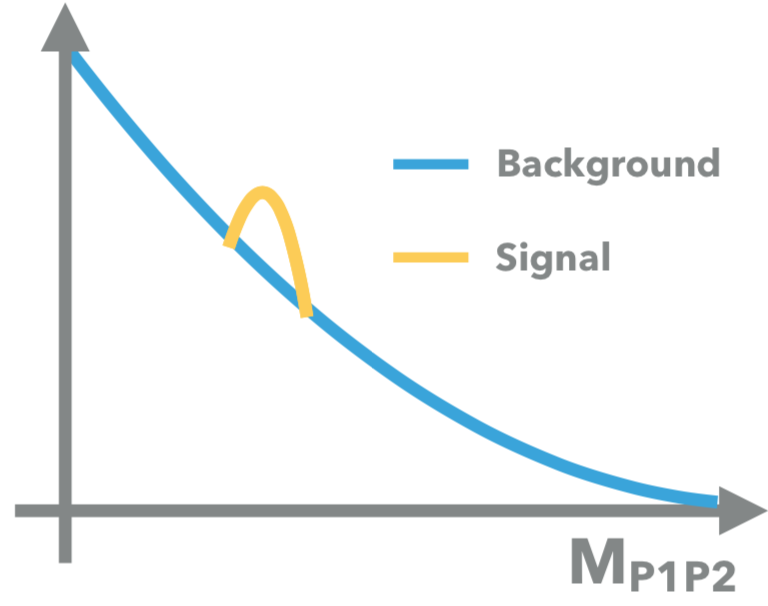
\includegraphics[width=0.75\textwidth]{figures/chapter_analysismethod/resonance}
        \caption{
            This cartoon illustrates a typical resonance finding experimental signature in the resonance mass variable. 
        }
        \label{fig:bump}
    \end{center}
\end{figure}
\FloatBarrier

The chapter below provides a recipe for a resonance finding analysis: Monte Carlo generation(MC) is used to aid statistical procedure formulation. Its generations are detailed in Section~\ref{sec:MC}. Proper data preparation required for both the data and the MC before statistical analysis is discussed in Section~\ref{sec:dataprep}. The background estimation method and their verification tests are given in Section~\ref{sec:backgroundest}. The search for resonances as excesses is quantified statistically. Two separate statistical statements, one on excess finding, and the other one on signal strength upper limit setting are discussed Section~\ref{section:stats}. 

\section{Simulated Physics Events(Monte Carlo)}
\label{sec:MC}
Simulated physics events(Monte Carlo) are used to design the cuts which optimize the selection, verifying the validity of the data-driven background estimation strategies as well as the different systematics.
An event generator used by ATLAS is PYTHIA~\cite{PYTHIA}, which is used to simulate the proton-proton collision, the tree-level generation, the hadronization, the fragmentation as well as the showering. 
Other than PYTHIA, the PowHeg generator~\cite{oleari2010powheg} and NLOJet++~\cite{nagynlojet++} are also used.
The detector effect is simulated by GEANT4~\cite{Agostinelli:602040}.

%It uses different \textit{tunes}, which are models and their parameters to estimate the effect of pile-up and the effect of simulated ``next-to-leading-order" showering. 


\section{Data Preparation}
\label{sec:dataprep}
The data of the analyses discussed in this chapter came from collision data, collected from the ATLAS detector and its triggering hardware and software discussed in Chapter~\ref{chapter:ATLAS}. The data collected as energy deposits and tracks are analyzed and collected analysis objects as discussed in Chapter~\ref{chapter:common_analysis_items}. After that, the dataset goes through several more steps in data preparation before getting analyzed for resonance finding in the chapter: the following is a short outline of how data are being prepared for the analyses.

First trigger chains addition is studied, balancing both events collected and signal sensitivity of the dataset studied. After that, the data is processed with the optimal analysis object working points applied, then, event cuts are introduced to maximize the signal sensitivity while reducing the background events. Later, binning on the target spectrum(in the case of analyses in this thesis, the resonance mass spectrum) is selected, balancing factors of optimal detector resolution and signal sensitivity(discussed in
Section~\ref{sec:binning}). Finally, a cross-check that compares the data and MC is performed variable regions other than the targetted spectrum. An a agreement between MC and data ensures both the previous steps in data preparation are executed correctly and the MC modelling is close enough to data descriptions. After all the data preparation steps are completed, a target signal spectrum is available to be analyzed statistically for resonances. 

\subsection{Binning Strategy} 
\label{sec:binning}

The target spectrum is binned for the resonance hunt. The bins are chosen to be narrower than the width of the expected signal, as this would lower the probability of mistaking fluctuation in a single bin as excess.

The binning is optimized through the mass resolution of the target spectrum. Since mass resolution describe the maximal sensitivity seen in the target spectrum, binnning is often chosen to be factors of the maximal resolution. This avoid the lost of information and allow the signal bump to be wider. 
The mass resolution is found through MC studies. As its main contributor is the detector effect, it can be studied through by performing a Gaussian fit on the $m^{reco}-m^{truth}$ on MC sample, where $reco$ is reconstructed event from GEANT4, and $truth$ is the truth events showering and detector reconstruction from the same event.
A Gaussian fit is performed to find the mean ($\mu$) and the width($\sigma$). The width found for the particular reconstructed mass is the resolution at that mass. 

%A uniform binning is chosen for the dimuon analysis, as it would make the background estimation more simplified. For the dijetISR analysis, to cope with the low statistics in the high mass region, variable bin size based on detector resolution is used. 

\section{Background Modeling}
\label{sec:backgroundest}
After the dataset has been prepared, the spectrum is ready to be analyzed to search for resonances. In order to analyze statistically whether there is an excess of events beyond the Standard Model prediction, a reliable prediction of the Standard Model events in the signal region along with its statistical error is needed. The step to estimate background Standard Model events is known as background modeling.
Many considerations go into background modeling for analysis: accuracy, availability, size of the estimation error and ease of implementation. In ATLAS, the following methods are recommended for background modeling in order of descending preference:
    First, the background estimation can be found by the MC generation of the events when the simulation is reliable and inexpensive for data generation. Second, in cases where the MC generated is low in event count but reliable in shape, an alternative estimation could be executed by scaling up the template from MC. In the case of the two analyses presented in this thesis, neither are there enough MC events nor are the shape of the MC event physically reliable. Thus, another class of methods of background estimation needs to be explored, all relying on the ``smoothness" feature of the background events. These include the fit function method, the expanded sliding window fit method(SWiFT) and the Gaussian Process method~\cite{frate2017modeling}.
    In the following section, the fit function method, the SWiFT method and the Gaussian Process method are discussed.

\subsection{Fit Functions/Global Fit}
\label{sec:fitfunction}
A class of fit functions are used to describe the distribution of the reconstructed mass due to smooth background. The most commonly used forms are cited as the following~\cite{ATL-PHYS-PUB-2020-028}. The selected fit functions are all resistant to capturing localized excess.

    \begin{itemize}

    \item \textbf{Polynomial}
        \begin{equation}
            f(m)= a_0 + a_{1}m + a_{2}m^{2}+...
        \end{equation} Here, m is the resonance mass, and $a_{i}$ are the different parameters.
    \item \textbf{Power Laws}
        \begin{equation}
            f(m)= a_{0}m^{b}
        \end{equation}

    \item \textbf{Exponentials}
        \begin{equation}
            f(m) = a_{0}e^{-b_{0}m} +a_{1}e^{-b_{1}m}+...
        \end{equation}
    \end{itemize}

From the above foundation, a list of historic fit functions has been developed over the years~\cite{Pachal:2063032}.
    %TODO cite 

    \begin{equation}
        f(m)=\frac{p_{0}}{m^{p_{1}}}e^{-(p_{2}m+p_{3}m^{2})}
    \end{equation}See~\cite{UA2:1990gao} for details.

    \begin{equation}
        f(m)=\frac{p_{0}}{m^{p_{1}}}(1-\frac{m}{\sqrt{s}})p_{2}
    \end{equation}See~\cite{1995} for details.

    \begin{equation}
        f(m)=\frac{p_{0}}{m^{p_{1}}}(1-\frac{m}{\sqrt{s}}+)p_{2}
    \end{equation}See~\cite{b582dc2d9c234174bfe2adbc9729bf42} for details.

    \begin{equation}
        f(m)=p_{0}(1-x)^p_{1}x^{p_{2}+p_{3}ln(x)}
    \end{equation}See~\cite{2009} for details.

    \begin{equation}
        f(m)=(1-x)^{p_{0}}x^{p1+p2ln(x)}
    \end{equation}See~\cite{2014} for details.

    In these fit functions, m is the resonance mass, p are the parameters, and x is defined to be $\frac{m}{\sqrt{s}}$.

\subsubsection{Cross-validation}
K-fold cross validation is often used to ensure the fit function is chosen correctly. In the procedure, the original dataset is divided into k different equal event size subsets through a random draw from the original dataset. Each of these subsets is tested by the candidate fit function and validated on the validation set. The best fit is chosen by averaging the p-value of the fit test statististic, $\chi^{2}/NDF$. The best fit is defined to have a p-value of the closest to 0.5.

While the fit function is relatively easy to implement, it is highly restrictive for complicated background shapes since it is low in flexibility~\cite{ATL-PHYS-PUB-2020-028}. When the increased luminosity of the LHC dataset leads to difficulties in fitting the background accurately, SWiFT and Gaussian Process are developed for the challenge. 

    \subsection{Sliding window fit(SWiFT)}
    When the simple fit function failed to model the data, SWiFT can increase the fit flexibility and the degree of freedom by fitting multiple narrower windows rather than the entire spectrum. The SWiFT window fitting procedure is summarized as below:
    
    1. A global fit is performed in the overall spectrum. Only when the overall $\chi^{2}$ p-value is below the fit threshold, SWiFT is attempted. Otherwise, the procedure ends in this step and a global fit method will be used. 

    2. The SWiFT fit will start with the maximum sized window, which is the number of bins of the entire spectrum minus one. The window scan starts from the lowest mass region along the spectrum. A fit is performed in the window. This estimates the spectrum up to the middle point of the window.

    3. The window moves up by one bin along the resonance mass spectrum. Another fit is performed. The prediction up to the middle of the window is added to the prediction in step 2. 

    4. Step 3 is repeated, until the end of the spectrum is reached. The final fit is checked against the threshold p-value of the $\chi^{2}$. If the fit $\chi^{2}$ is below the designated threshold, the background estimation ends. Otherwise, the window size is further reduced by one bin, and step 2 and 3 are repeated until either a fit above the test statistic threshold is found or the minimum window size is reached. The minimum window size is defined by the signal injection test discussed
    below in Section~\ref{sec:signalInjection}.

    Figure~\ref{fig:swift} here shows a doodle on the sliding window method.
    While the SWiFT can provide extra flexibility to the fit, it is also prone to becoming too flexible the signal in data will be estimated as part of the background. To provide the most accurate background prediction while balancing signal sensitivity, SWiFT always aims to use the largest window possible that can still accurately describe the background. 

As the SWiFT window size is not selected until the data is unblinded, a carefully designed unblinding procedure is required. Figure~\ref{fig:unblinding} shows a sample unblinding procedure, as used in the dijetISR resolved analysis in presented in Chapter~\ref{chapter:dijetISR}.

\begin{figure}[!htb]
    \begin{center}
        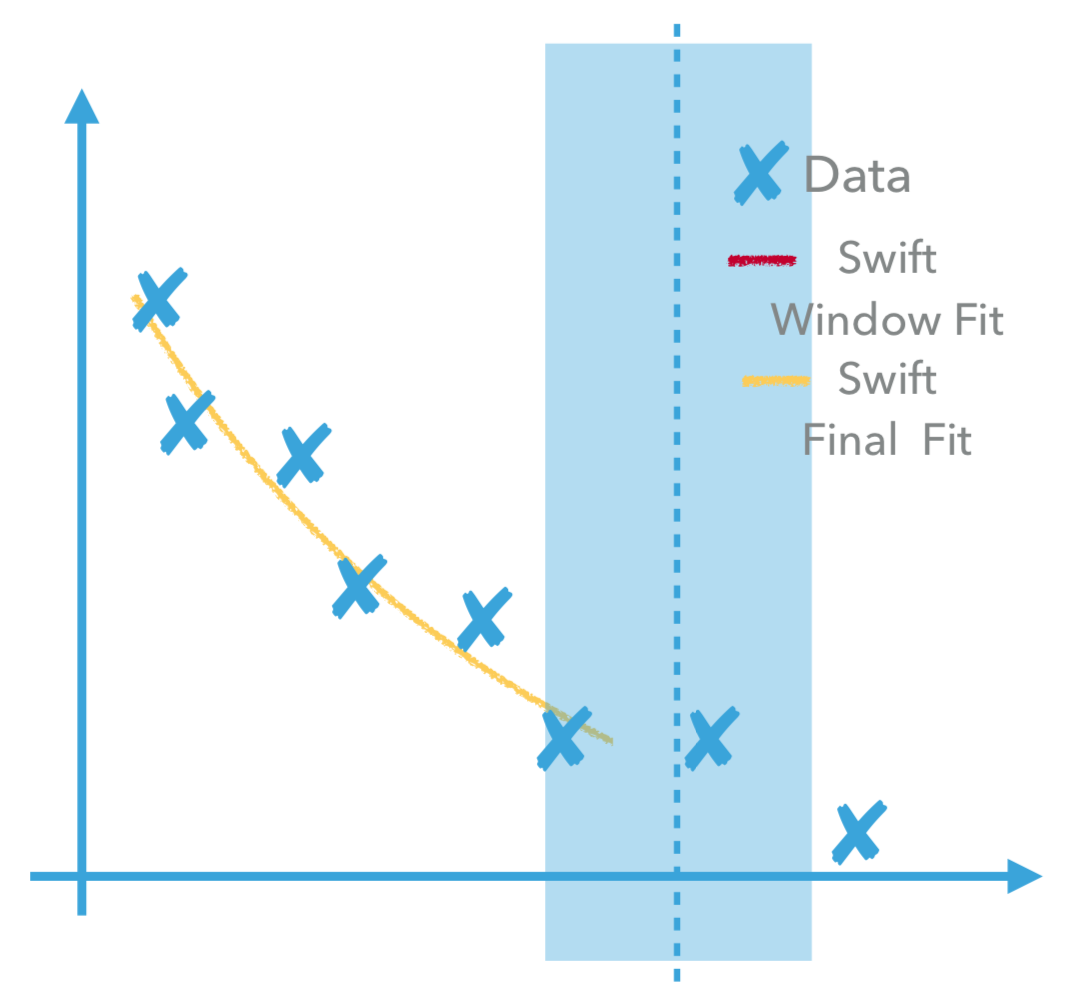
\includegraphics[width=0.75\textwidth]{figures/chapter_analysismethod/swift2}
        \caption{
            This figure shows a doodle on the procedure of the sliding window fit. 
        }
        \label{fig:swift}
    \end{center}
\end{figure}

\begin{figure}[!htb] \begin{center}
        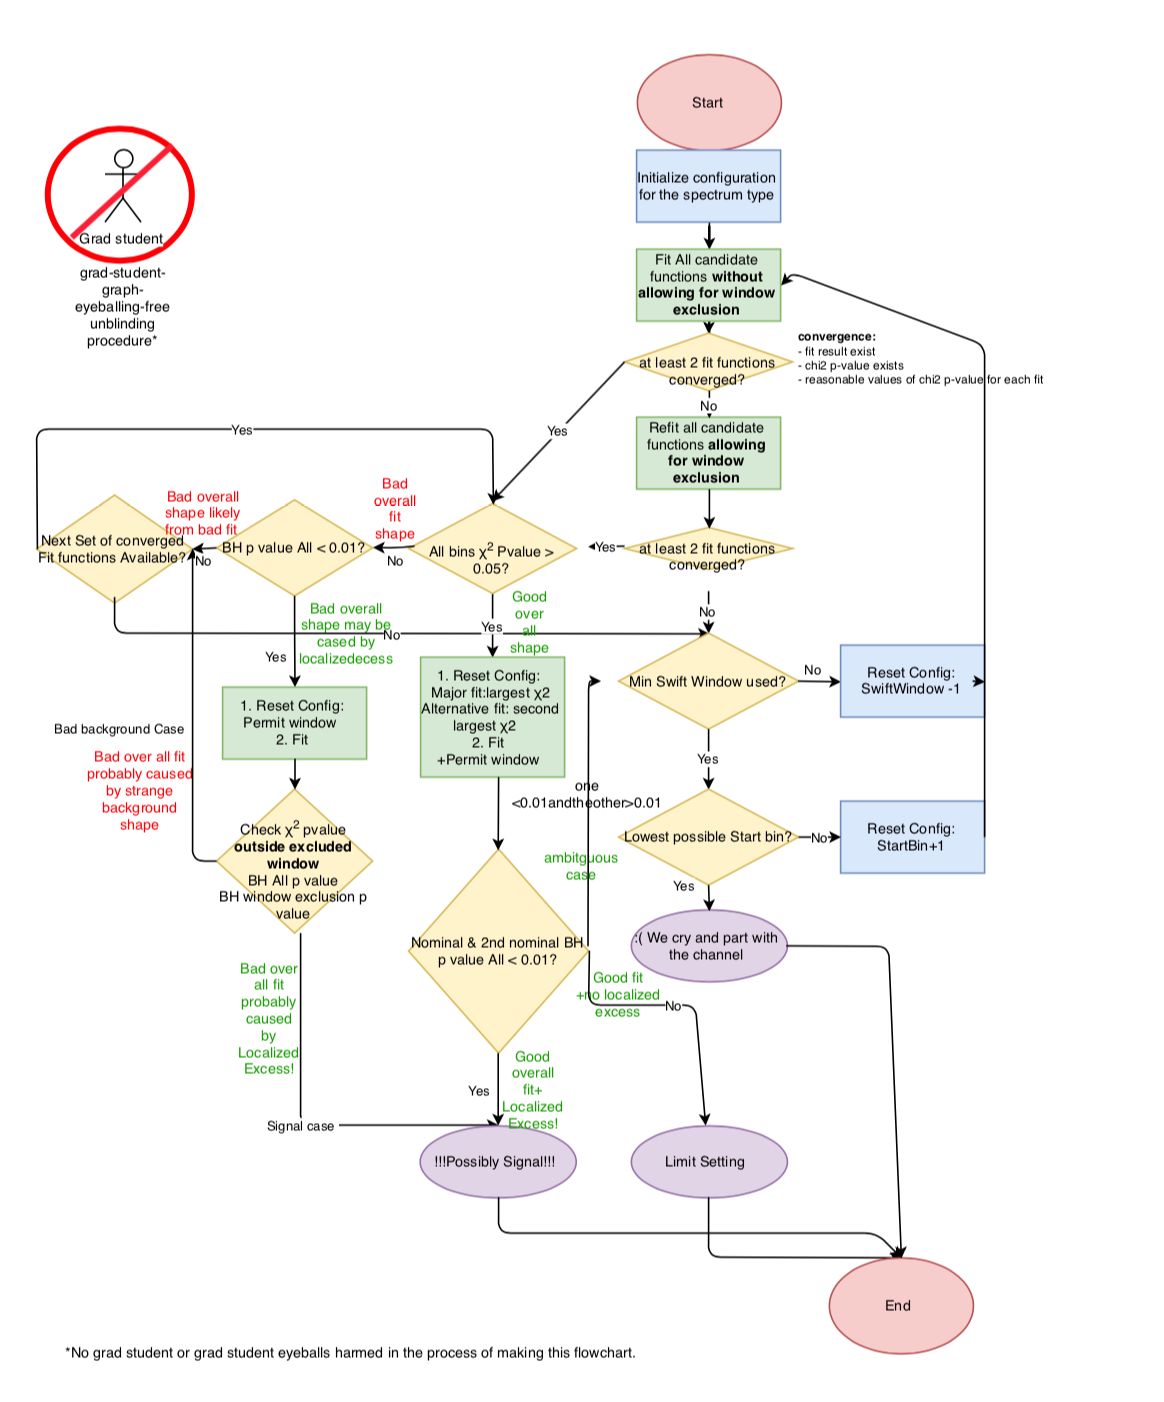
\includegraphics[width=1.05\textwidth]{figures/chapter_analysismethod/swift_unblindingflowchart}
        \caption{
            This figure shows a doodle on the procedure on the unblinding using SWiFT.
        }
        \label{fig:unblinding}
    \end{center}
\end{figure}
\FloatBarrier
    
    \subsection{Gaussian Process} 
    \label{sec:GP}

    Gaussian process background prediction is performed through Bayesian inference. The former estimation of the prior Gaussian joint probability distribution form more constricted posterior distribution with the added information from data. Unlike the above fit function-based method, Gaussian Process predicts an infinite number of functional forms, constrained by a kernel, which defines the bin-to-bin covariance.


    Gaussian process can naturally be applied to the background estimation of a spectrum since the bin event count in background and signal modeling are approximatedly a Gaussian distribution in each bin: In the resonance spectrum background, the prediction in every bin is a Poisson distribution due to its counting experiment nature. Poissonian distributions can be approximately described as a Gaussian Distribution through the Central Limit Theorem~\cite{kwak2017central}. As the distribution between the points is smooth, the relationship between each of the neighboring bins can be described by a joint distribution where the correlation is a covariance matrix. The covariance matrix can embed physics knowledge regarding the detector resolution and object energy scale. The Gaussian process allows for more flexibility in the functions compared to the above two methods, as can be shown here in this covariance matrix diagram:

    \begin{figure}[!htb]
        \begin{center}
            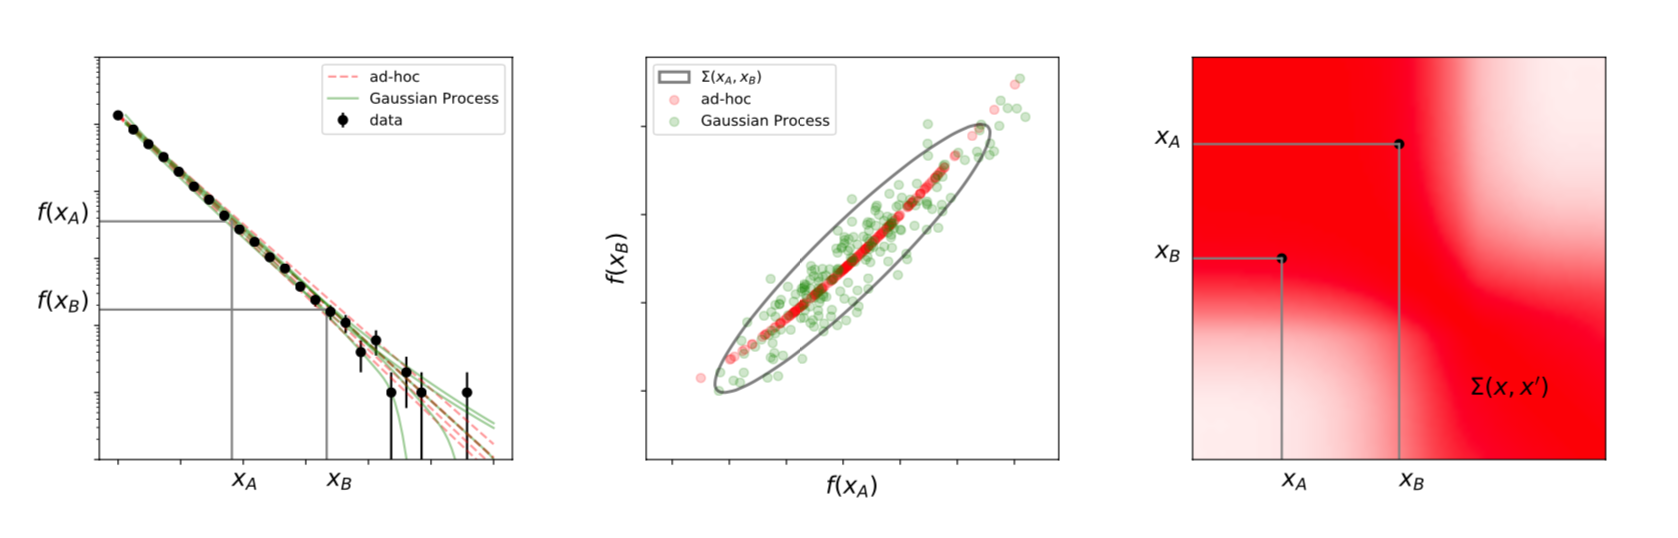
\includegraphics[width=0.7\textwidth]{figures/chapter_analysismethod/GP}
            \caption{
                These figure shows that the Gaussian process fit is able to provide more flexibility than the standard fit function method. The Red line in the first panel shows results from the fit function method and the green line shows the extra flexibility gained by Gaussian Process. The second pane shows that the possible value of the fit functions are relatively constricted (in red) compared to the Gaussian Process prediction (green) when the prediction are sampled at point $X_{A}$ and $X_{B}$. The black line shows the covariance matrix. The third pane shows the Covariant matrix of the kernel, where $X_{A}$ and $X_{B}$ are labeled. ~\cite{frate2017modeling}.
            }
            \label{fig:GaussianProcess}
        \end{center}
    \end{figure}
    \FloatBarrier


\subsubsection{Gaussian Process: Regression}

The Gaussian process background prediction method is a Bayesian method that predicts the posterior probability distribution. The mean function of this posterior probability distribution is the backgrdoun estimation prediction from GP, and the covariance matrix from it is the GP prediction error.

%where the prior distributions can be ``updated" by binning information. From Bayesian inference, a new prediction can be formed from the posterior. It can be shown that the mean and covariance can be given by the following formulae:

    \begin{itemize}

        \item \textbf{The Mean Function}

    \begin{equation}
        \mu(x_{*}|y)  = \mu(x_{*})+ K(x_{*}, x)[K(x, x)+ \sigma^{2}(x)I]^{-1}(y-\mu(x))
    \end{equation}
    Here, $\mu(x_{*}| y} $ is the mean function posterior prediction of of point $x_{*}$, given known data point x and y, K is the kernel, $I$ is the diagonal matrix, $\sigma$ is the white noise term in each bin. $\mu(x_{*})$ is the prior probability distribution. x is a vector of the input mass point, and x' are the same points in a 2d matrix.

    \item \textbf{The Covariance Function}
    \begin{equation}
        \sum(x_{*}, x_{*}') = K(x_{*}, x) - ((K(x_{*}, x')+\sigma^{2}I)^{-1)}[K(x, x')]
    \label{eq:covariance}
    \end{equation}  
    Here, the covariance is defined for $x_{*}$ and $x_{*}$, the data point where the predictions were made, x and x' where the input data points are given. K is the kernel of the Gaussian Process prediction.

    \end{itemize}

    Here, x and y are input data to constrict the distribution, $x_{*}$ is the points where the posterior GP are evaluated from, x' is the same points as x in a 2d matrix.

    \subsubsection{Gaussian Process: the Kernel}
\label{sec:kernel}
From Eq.~\ref{eq:covariance}, kernel is directly related to the covariance function in Gaussian Process. Kernel descibes how the relating neighboring points are related to one another. 
Various kernels are used for different analysis backgrounds with distinct features. A specific example to the dijet spectrum is demonstrated in ~\cite{frate2017modeling}.

%t's found that the simple radial basis function and a white noise kernel are sufficient to describe the background spectrum, the signal is described by another radial basis function kernel of a particular mean value.
%The kernels are given as the following: 
An other more general example is given as below.
%
    \begin{itemize}
        \item \textbf{Background Kernel}

            The background kernel is the addition of the Radial Basis kernel function plus the white noise kernel.
            \begin{equation}
                K_{bkg}(x, x') = A_{1} * exp(-\frac{||x-x'||}{2\sigma^{2}}) *+ K_{noise}
                \label{eq:backgroundkernel}
            \end{equation}
            Here, $A_{1}$ is the amplitude hyperparameter that describes the size of the kernel, $\sigma_{1}$ is the lengthscale parameter.
            The noise kernel is a constant diagonal kernel:
            

			\begin{equation}
            K_{noise}(x_{i}, x_{j}) =
			\begin{cases} \text{noise level} & \text{if $x_{i}==x_{j}$,} \\
			\\
            0 & \text{otherwise.}
			\end{cases}
			\end{equation}

        \item \textbf{Signal Kernel}

            The signal kernel is a square centered exponetial kernel
            \begin{equation}
            K(x_{i}, x_{j})=A_{2}\cdot exp(-(x-m)^{2}/(2\cdot\sigma_{2}^{2}))\cdot exp(-((x'-m)^{2}/(2\cdot\sigma_{2}^{2}))) + K_{noise}
            \label{eq:signalkernel}
            \end{equation}

    \end{itemize}
            Here, $A_{2}$ is the amplitude of the signal kernel, m is the value where the kernel peaked on, and $\sigma_{2}$ is the lengthscale of the signal kernel. 

	Of all the hyperparameters, lengthscale(\sigma) is given special attention as its value descirbes how much neighboring points affect prediction at any given point. Its special treatment is described in the following sections.

    \subsubsection{Gaussian Process: Hyperparameter Optimization}
    \label{sec:hyperparam}
    %The lengthscale($\sigma$) hyperparameter in both kernels(See Eq.~\ref{eq:backgroundkernel} and Eq.~\ref{eq:signalkernel}) is prone to overfitting when the chosen value is too small. This would lead to reduced signal sensitivity and the overfitting of statistical fluctuation. A lower bound is set in these hyperparameters: The lower bound in the background kernel lengthscale is determined by the signal injection test described in Section~\ref{}; the lower bound in the signal kernel lengthscale
    %is chosen through the binning studies in Section~\ref{sec:binning} respectively. 
    Kernels are parametetrized by hyper-parameters. Hyperparameters are higher level parameters that controls and aid the learning of the process through input of data. %In fitting of a mass spectrum and its signal. The kernel hyperparameters are allowed to float and the final values are optimized through the scaled conjugate gradient algorithm, which minimizes the negative log marginal likelihood of the Gaussian Process:


	The lengthscale hyperparameter, with its special nature, has a lower bound set on it through the signal injection test described in Section~\ref{sec:signalinjection}. The minimization of the hyperparameters is performed through a scalar conjugate gradient search. To avoid reaching a local minimum, the initial values of the hyperparameters are chosen through a grid before the minimization. The minimized hyperparameter are compared to the other sets. The set of value with the overall lowest negative log likelihood is chosen to be the optimal hyper-parameters.

    \begin{equation}
        -\ln(L) = -\frac{1}{2} ln |\sum| - (y-\mu(x) ) - \frac{n}{2}\ln(2\pi)
    \label{eq:loglikelihood}
    \end{equation}
    

    In this Gaussian process testing procedure, the hyperparameters are first found on a test fit on the variation of MC, the fixed hyperparameters are then applied to data.
%
\subsection{Background Fitting Tests}
Following the ATLAS smooth background recommendation~\cite{ATL-PHYS-PUB-2020-028}, the following tests are performed to ensure the validity of the background estimation for resonance searches.

\subsubsection{Signal Injection Test}
\label{sec:signalInjection}

    Increasing the number of parameters in a fit function, using smaller windows size in SWiFT, or using a background kernel lengthscale in the Gaussian Process all increases flexibility in modeling the background. However, the increased flexibility in background modeling often comes with the price of decreased signal sensitivity. An overly flexible background estimation would fit the signal away as part of the background. 
    Therefore a test to quantifies the signal sensitivity of the background estimation is necessary. The test is called the signal injection test. On ATLAS, it is required that the background modeling provides sensitivity to signals of at least 3 $\sigma$ of the background error.

    The background error is defined by the generation of 10,000 bin-by-bin Poissonian toys from the original background MC spectrum, and by refitting the toys by Gaussian Process background kernel estimation. A Gaussian fit is performed on the prediction of each bin, the resulting width of the Gaussian fit in each bin is defined to be the 1 $\sigma$ background estimation. 

    %defined by the width of the Gaussian envelope from the pseudoexperiment fits. The background estimation passes the signal injection test when it passes such requirement.

    In addition to quantifying signal sensitivity, the signal injection test is used to constrain the lower bound of the lengthscale in Gaussian Process and SWiFT window size. The window size or lengthscale value is restricted by to a lower bound that would return a background estimation that provides sensitivity to signals of at least 3 $\sigma$ background error in size.

    Signals of different mass widths are generated from a Gaussian distribution. Poissonian noise is thrown randomly on the distribution to create a pseudo signal distribution. The mass widths are chosen to be 1\%, 3\% and 5\% respectively. Signal of different scales with corresponding error is generated and is injected into the background MC distribution.

    For each chosen maximum lengthscale/SWiFT window, and different signal widths, the below is performed with the bumphunter.

   1. First a background fit is performed on the background MC distribution, the bump-hunting~\cite{choudalakis2011hypothesis} procedure is performed as described in the above section. If the overall bumphunter p-value are below the critical value for window exclusion, the next step is performed. Otherwise, the background fit strategy has to be reviewed. A different fit function or Gaussian Process kernel is needed.

   2. A small signal is injected in the background MC distribution, a fit is reperformed, and the bumphunter window and overall p-value is calculated again. 

   3. An increasing signal size is injected into the spectrum and step2 is repeated until a signal of size large enough to lead to a small enough bumphunter statistic p-value.(The test statistic is defined in Section~\ref{teststatistics}) When the p-value is below 0.01, window exclusion in the bumphunting procedure is triggered. The signal size injected just before the window exclusion is the largest signal the search is not sensitive to. The minimal signal size injected that triggers the window exclusion is the smallest signal size that the search is sensitive to. 


%Starting with the smallest signal size and the smallest width, the bumphunter procedure detailed in section~\ref{} is ran on the signal injected background MC. The signal size injected increases, until the bumphunting procedure finds a window with bumphunter statistic p-value $<$ 0.01 that a bumphunter window exclusion is triggered. The size of the signal injected right before the window exclusion triggering is the ``just below"
%triggering signal size, and the signal size that triggers the window exclusion is known as the ``just above" signal size. The "just below"
%window size is the largerst signal that the background estimation is not sensitive to; and the ``just above" signal size is the smallest signal that the background estimation is sensitive to. When the background kernel lengthscale is chosen to be 4 GeV, the background model is sensitive to signal 3 $\sigma$ or above in background error. 
%

%\begin{figure}[!htb]
%    \begin{center}
%        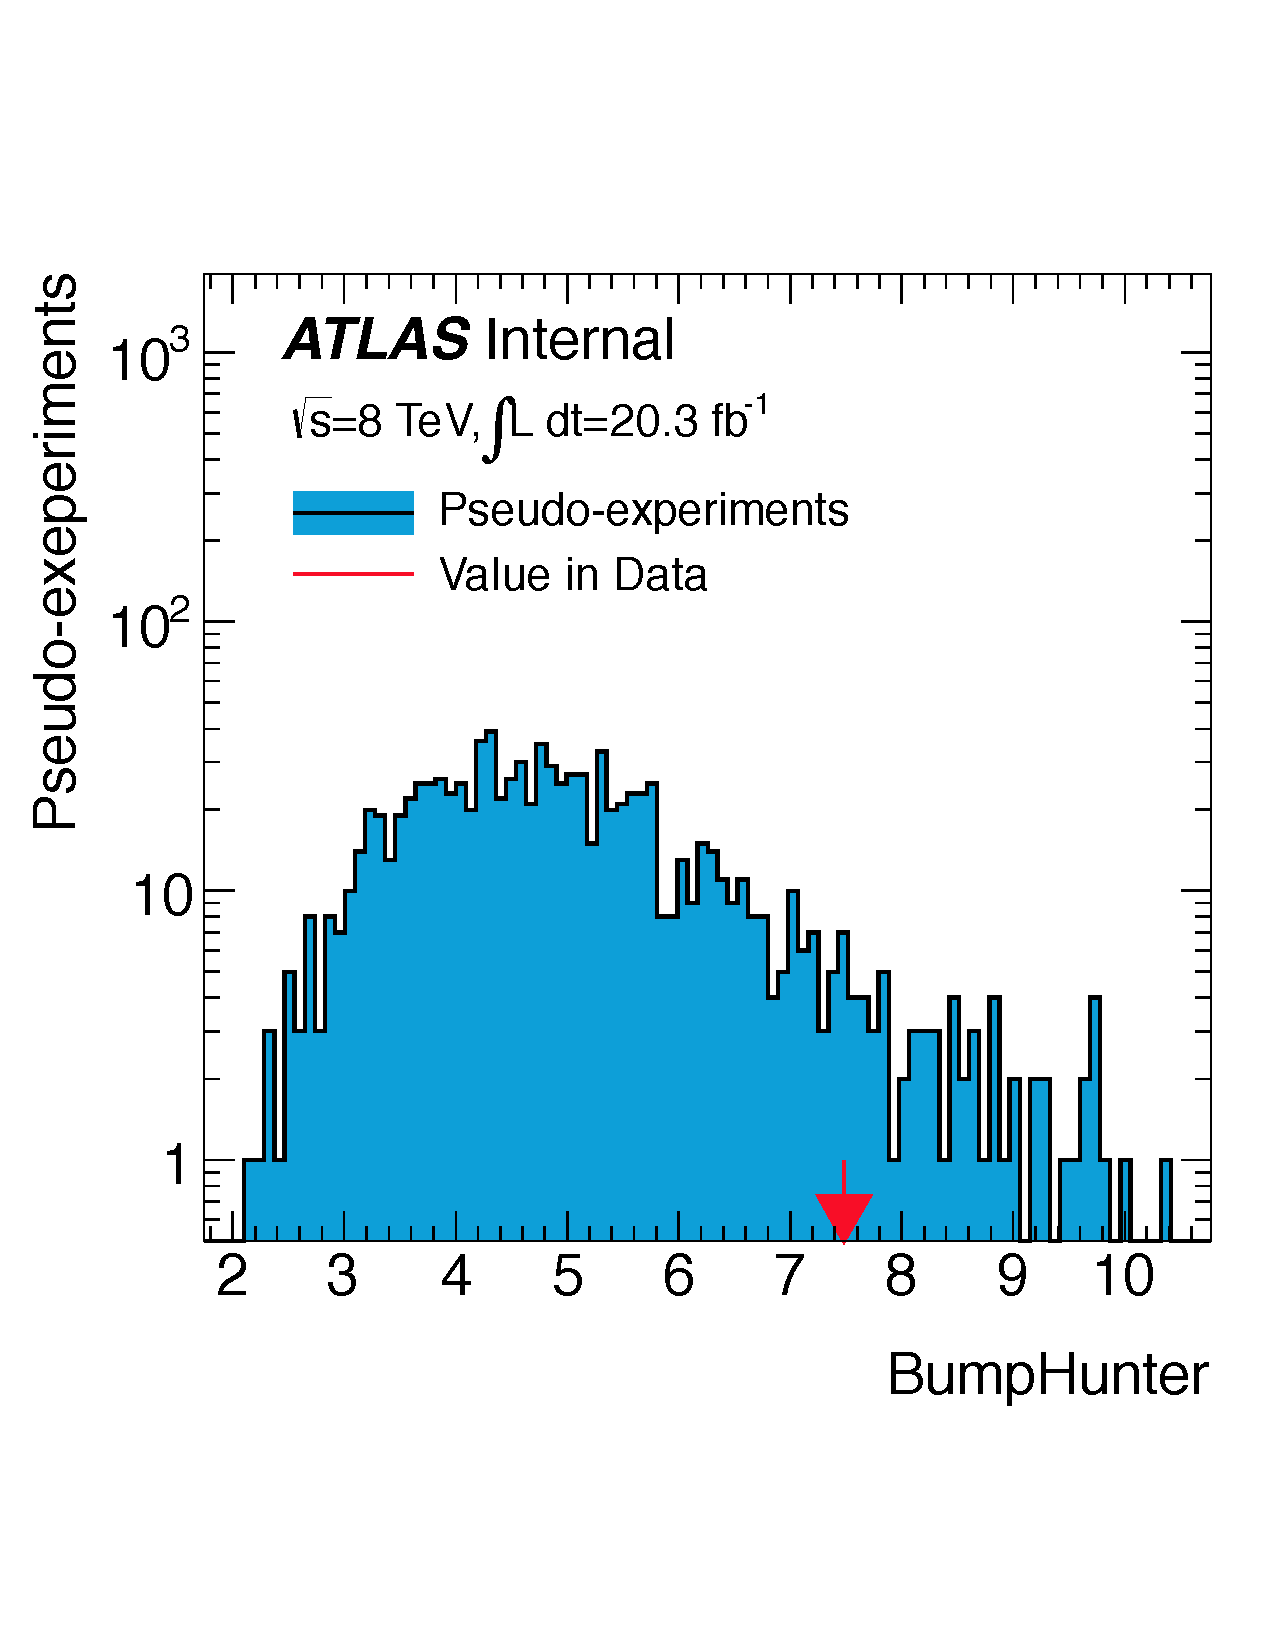
\includegraphics[width=0.75\textwidth]{figures/chapter_analysismethod/bumphunter}
%        \caption{
%            This diagram shows the bumphunter test statistics distribution, where the red arrow shows the observed value. 
%        }
%        \label{fig:teststats}
%    \end{center}
%\end{figure}
%\FloatBarrier
   
   %The background fit, or parametrically, the SWiFT window size/Gaussian process lengthscale, is said to have passed the test if the largest signal the search is not sensitive to is within 3 $\sigma$ of the background error bands. 

   %The smallest lengthscale value/SWiFT window size where the largest signal the search is not sensitive to stays in the error bands is the minimal SWiFT window/Gaussian Process fit value that can be used during unblinding. 

\begin{figure}[!htb]
    \begin{center}
        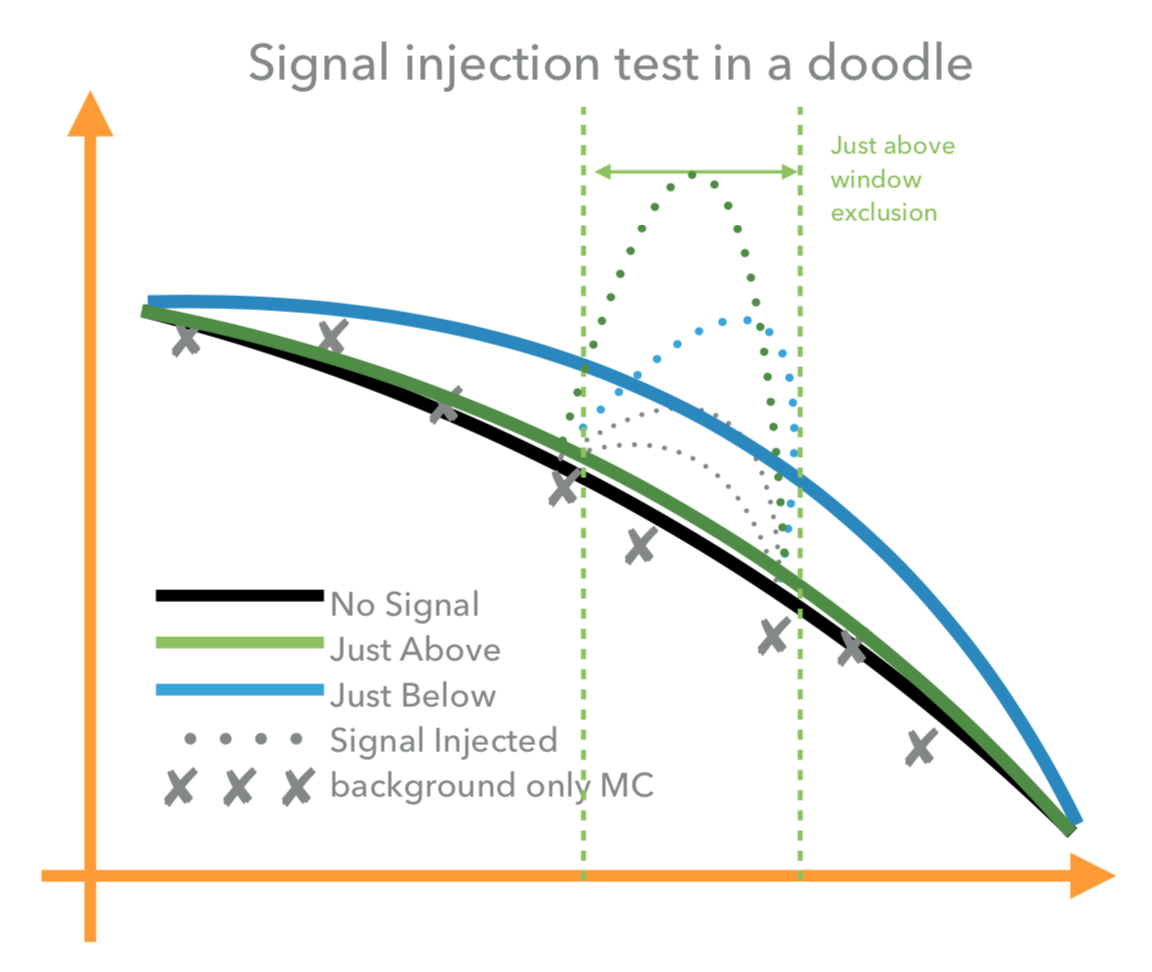
\includegraphics[width=0.7\textwidth]{figures/chapter_analysismethod/SignalInjectionTest}
        \caption{
            This figure shows a doodle of the procedure of the signal injection test. An increasingly large signal is injected to the background MC spectrum until the window exclusion procedure of bumphunter is triggered.
        }
        \label{signalinjection}
    \end{center}
\end{figure}
\FloatBarrier

\subsubsection{Spurious Signal Test} 
    \label{sec:spurious}
    %\epigraph{\textit{-``Test for signal extracted from the background estimation alone"}}

    To measure the amount of possible false signal in the background modeling method, the spurious signal test is performed. The spurious signal test models the amount of signal that the background plus signal fit when no signal is present.  It statistically quantifies the stability of the background estimation. It is also sometimes used as a measure of the background fit error.

Using the different variations of background only MC spectrum, a signal plus background fit is performed, the signal extracted is compared against the background error defined in the last section. The spurious signal test is considered passed if the signal extracted versus the background error ratio is $<$ 0.5.

    The spurious signal is defined as the following:
    
    \begin{equation}
        S_{spur} = S_{fit} - S_{template}
    \end{equation}

    Here $S_{fit}$ comes from the signal fit component of the background + signal fit, $S_{template}$ changes with the kind of analysis being performed. It is set to be 0 for a search.     
    %The median of the 10000 pseudo experiment fit is taken to be the spurious signal value. 
    %In the figure below, a sample spurious signal fit is shown~\ref{spurioussignal}.
    %In general, the spurious signal has to stay within 50\% of the background error bands, defined as the error bands generated from the fitting of 10000 background MC pseudo experiment from the Poisson distribution with the background fit only.
    %If the background fit stays within the 50\% requirement, it passes the spurious signal test.

\begin{figure}[!htb]
    \begin{center}
        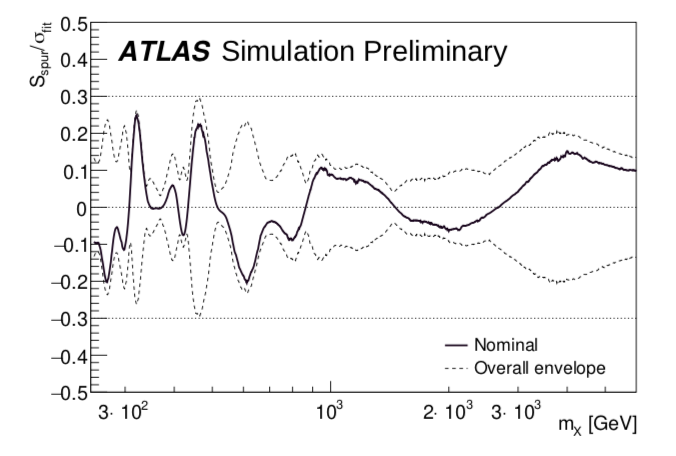
\includegraphics[width=0.75\textwidth]{figures/chapter_analysismethod/Spurious}
        \caption{
            This figure shows the example results of a spurious signal test. Here, the error $\sigma$ is defined as $\sigma_{tot} = \sqrt{\sigma^{2}_{fit}+ S_{spur}^{2}}$ ~\cite{ATL-PHYS-PUB-2020-028}.
        }
        \label{spurioussignal}
    \end{center}
\end{figure}
\FloatBarrier

After the data preparation steps and tests performed on background estimation. The mass spectrum and estimation are both ready for statistical testing for possible resonances. 

\section{Statistics Testing}
\label{section:stats}
Statistical testing is the quantification of whether an excess is seen or what experimental bound can be drawn from the final analysis. 

The statistics testing on a hypothesis can be presented as a test on the significance Z: 

\begin{equation}
 Z= \Phi^{-1}(1-p) 
 \label{eq:significance}
\end{equation}

Here, p is numeric probability representation of the agreement between the data and the model given a hypothesis. $\Phi$ is its conversion of the p-value into quantile of a cumulative Gaussian distribution. From here on, Z will be referred to as the significance and p will be referred to as the p-value.

There are two distinct statistics tests in a typical resonance search analysis. Each test is compared to a threshold value of Z. The two tests will be referred to as ``the search" and the ``limit setting". Details are described in the following sections.

%Before the Here, the null hypothesis is the hypothesis that include only known processes from the Standard Model hypothesis with no excess; the alternative hypotheis is the hypothesis that include both background and signal of a certain signal strength.

%\begin{itemize}
%    \item \textbf{1.  The Search}
%()corresponds to $p = 2.87 \cdot 10^{-7}$.


%the Bayesian tool is used for the dijetISR analyses, whereas the frequentist method is used for the dimuon analysis. 
%\end{itemize}

\subsection{The Search}
\label{sec:thesearch}
%\epigraph{\textit{-``The Rejection/Acceptance of the null hypothesis"}}

The search aims to look for model independent statistical excesses present in data. This test is implemented in comparison to the null hypothesis, where it is defined to be the Standard Model prediction. The search is implemented in a frequentist manner through the Bumphunter method~\cite{choudalakis2011hypothesis}. This section describes the statistics principle behind this test and details the bumphunting procedure. 

%From comparing the data test statistics value to pseudoexperiement, if the significance Z $>$ 5, the null hypothesis is rejected. Something beyond the Standard Model is observed in the data to a statistically significant degree, otherwise, the Standard Model prediction is accepted. In the Higgs boson analysis of 2012, a significance of Z $>$ 5 was observed in the search.


\subsubsection{The Search: The Statistics Principles}
The probability of having made a measurement in each bin can be described by a probability distribution. As each bin is considered an independent event in a fixed data-taking period and physical variable value. The probability distribution takes the Poissonian probability distribution form:

\begin{equation}
 P(x=k|\lambda) = \frac{\lambda^{k}e^{-\lambda}}{k!} 
 \label{eq:Poissonian}
\end{equation}

Here, $\lambda$ is the expected value of the measured quantity $x$, $k$ is the number of occurrences, e is Euler's number.

The test is implemented in a frequentist manner. It compares the observation outcome x with a fixed critical value $\alpha$ of a probability distribution generated from pseudo-experiment. The value used to reject or accept the null hypothesis is quantity called the p-value. Statistically, it is known to be a false-discovery probability(See Eq.~\ref{eq:test}). If the observation compared with the pseudo-experiment distribution is smaller than the critical p-value, the null hypothesis is rejected. The rejection criteria can be shown in the following mathematical form:

\begin{equation}
    P(x \ni w|H_0)<= \alpha 
    \label{eq:test}
\end{equation}

Here, $H_0$ is the prediction from the null hypothesis, and alpha is the critical value below which the null hypothesis will be rejected. The value is usually taken to be 0.01 for the bumphunter experiment. It corresponds to a probability of 1\%. $x$ is the observed value out of all possible outcome $w$.  

\subsubsection{The Search: Test Statistics}
\label{teststatistics}

The test statistic is a function of the observable $x$, the p-value in~\ref{eq:test} can be rewritten as:
    
\begin{equation}
    p = P(T>=t_{0}| H_{0})
\label{eq:pvaluetestStats}
\end{equation}

Here, $H_0$ is the null hypothesis, $t_0$ is the test statistic of the null hypothesis, and T is the observed test statistic.

Equation~\ref{eq:pvaluetestStats} evaluate the p-value of the observed value. T is a function of the observed $x$ in the window. It's the probability of the observed test statistics obtaining a value at least as extreme as $t_{0}$. A small p-value refects a poor agreeement between the observed T value and the hypotheis $H_{0}$.

Various test statistics are available to quantify the level of agreement between an observation and a hypothesis. If the test is concerned with overall agreement between data and the model, the $\chi^{2}$ test or the log-likelihood of the Poissonian distribution are fitting candidates.

The bumphunter test statistics instead quantifies localized excesses, the test statistics is defined in a window and calculated for the bins within. It is a more powerful test for the kind of deviation expected in resonance hunting.

In a window defined from bin number m to n, the observed data and prediction can be given as the following: 
    \begin{equation}
         d= \sum_{i=m}^{n} d_i 
    \end{equation}

    
    \begin{equation}
         b= \sum_{i=m}^{n} b_i
    \end{equation}

    Here d is the total number of events in the window observed, where $d_i$ is the count in each of the bins from m to n. 
    Here b is the total number of events in the window predicted, where $b_i$ is the event count in each of the bins from m to n.
    
    Assuming the observed counts in each bin follow a Poissonian distribution, the test statistic is:

\begin{equation}
    t^{\textrm{BH}}=
    \begin{cases} \sum_{n=0}^{d} \frac{b^{n}}{n!} e^{-b} &  \textrm{for $d < b$}
    \\
    \sum_{n=d}^{\infty} \frac{b^n}{n!} e^{-b} &  \textrm{for $b \leq d$}
    \end{cases}
\end{equation}

    The above expression can be represented by the Gamma function($\gamma$): 

\begin{equation}
    t^{\textrm{BH}}=
    \begin{cases} 1-\gamma(d+1, b) &  \textrm{for $d < b$}
    \\
    \gamma(d,b) &  \textrm{for $b \leq d$}.
    \end{cases}
\end{equation}
    

    The p-value of the bumphunter test statistic is evaluated for every windows from two-bin wide to half the spectrum($t^{\textrm{BH}}$). The overall bumphunter test statistic is defined by the to be the log of the smallest p-value calculated from the smallest p-value window, and can be represented as the following($t^{\textrm{BH}}_{0}$):

%    \begin{equation}
%        t_{0}^{\textrm{BH}} = - \ln(t_^{\textrm{BH}}_{\textrm{min}}) 
%    \end{equation}

    Significance Z and the p-value can be calculated from this test statistic in Eq.~\ref{eq:pvaluetestStats} and thereby provide an overall bumphunting hypothesis could have generated data this unlikely or more. If the p-value is lower than 0.01. %the null hypothesis is rejected, otherwise, it is accepted.

    %In addition to the bumphunter test statistics, there is the tailhunter, KS, Jeffreys and no sidebands bumphunter that can also be chosen for different signals searched for in other physics analyses. More information can be found in the Bumphunter paper\cite{choudalakis2011hypothesis}.

    \subsubsection{The Search: The Bumphunting Procedure}
    % Look up the bumphunter fit. 
    The bumphunting procedure is defined to look for excesses as defined by the bumphunter statistics~\cite{Pachal:2063032}.

    1.  First a background model fit is performed. (See Section~\ref{sec:backgroundest}). The $\chi^{2}$ of the fit is verified to have a p-value $>$ 0.01. Otherwise, the fit will be revised or moved to an alternative method.

    2.  If the background fit passes the $\chi^{2}$ test, the bumphunting test can begin. In all defined windows, bumphunter test statistic and their p-values are calculated. If the overall bumphunter test statistic has a p-value above 0.01, stop, no excess is found. Alternatively, if any one of the windows has  $p< 0.01$, the window most discrepant window (the window with the lowest p-value) is removed, and the fit is reperformed. If the new fit with the window removed has a p-value above 0.01, it shows the discrepancy is completely contained in the window removed.

    3. After reperforming the fit with the window removed, if an overall bumphunter statistics p-value is found to be over 0.01, Stop. A local discrepancy may have been discovered in the removed window. Otherwise, if the newly discovered most discrepant window is adjacent to the window removed, it demonstrates that the signal peak may still be outside of the window, one more bin of window exclusion will be added to the removed window. If the newly discovered most discrepant window is not adjacent to the window removed, one bin of each side is added to the original removed window. The fit is re-performed with the new window removed. This step is repeated until either the p-value of the fit with the removed window has a p-value above 0.01, or no additional window could be added to the exclusion because all bins has been added to the removal window.

    Summarizing from the above, three end results are possible in the search test:

    1. If no window is excluded and the fit has a bumphunter p-value statistics above 0.01. No excess is found. 

    2. If there is one excluded window and a background fit with a bumphunter statistics p-value of above 0.01. An excess up to a certain significane is quoted.

    3. In all other scenarios, more tests are required. The background model fit could be problematic and need further testing.  

\section{Limit Setting}
\label{sec:limits}

%\epigraph{\textit{Finding signal strength value where the alternative hypothesis is rejected to a 95\% confidence level}}

Statistically, the upper limit setting is the finding of the signal strength where the alternative hypothesis is rejected at a 95\% confidence level. The signal strength can also be represented as a cross-section or cross-section in fiducial volume for reinterpretation for different models. 
The limit setting results consist of a 95\% confidence upper limit bound on signal strength over the resonance masses and an expected limit of median significance along with statistical uncertainties with the null hypothesis. 
%It is possible to compare the observed 95\% upper limit against the expected limit. The comparison between the bands and the upper limit line can be seen as a discovery test, as if no beyond the Standard Model excess is seen, the upper limit line would stay between the 5 $\sigma$s error band in the expected limit. 

The limit setting can be performed in two different ways, the Bayesian statistical way and the frequentist way. While the interpretation and implication of the results made with the different methods are different, the results produced are designed to be comparable across different analyses. 

The Bayesian method is used for the dijetISR analysis(Chapter~\ref{chapter:dijetISR}) and the frequentist method is used for the dimuon analysis(Chapter~\ref{chapter:dimuon}). A description of the dimuon frequentist limit is given as below. 
%The 95\% confidence level corresponds to a critical p-value of 0.05 or a Z value of 1.64.

%The limit is a hypothesis testing procedure that test both the compares the null hypothesis of absence of signal ($H_{0}$) to the hypothesis where there is a signal($H_{1}$). 
%The limit is a projection of the $H_0$ and $H_1$ hypothesis in either the cross-section or the signal strength axis. This provide another way to discuss signal discovery, and information on an 95\% confidence limit in the If $H_1$ shows agreement with $H_{0}$ when fluctuation is taken into account, the 
%Even in the absence of a signal, a statement can be made about the signal strength value that is ruled out by the signal+background. 
%
%The limit setting procedure can be done in both the frequentist and Bayesian way on ATLAS, and in the analyses presented, the dimuon analysis is done in the frequentist way, whereas the dijet analysis is done in the Bayesian way. 

%\subsection{Bayesian limits}


\subsection{Frequentist Limits}
\label{sec:freq}
The limit is a statement on where the observed data lies given all the other possible outcomes given a hypothesis. The 95\% CL upper limit is result of a procedure which if run in hypothetical similar experiments would include (exclude) the true value 95\% (5\%) of the time.

The following subsection describes the test statistics used for the limit setting. A formulation of the traditional frequentist calculation is presented. The Asimov approximation method used to approximate the frequentist limit from a representative dataset is described, which is the ATLAS standard, and it saves computing resources. The formulae for the limit calculation using this method are given. Adaptation with the Gaussian Process is also discussed. 

\subsubsection{Frequentist Limits: The Test Statistic}
\label{sec:freqTestStats}

The probability distribution of the observable $x$ in each bin of the histogram can be given by a Poissonian probability distribution. This probability distribution is a function of many parameters, including the signal strength, and other systematic uncertainty parameters, for example, the variation in luminsoity. As these variable are not the target parameter where limit is set, they are known as the nuissance paramters. From the Poissonian distribution, its likelihood function can be parameterized as such, with thepredicted signal event and background events made explicit:

\begin{equation}
    L(\mu, \theta) =  \prod_{i=0}^{N} \frac{(\mu \cdot s_{j} + b_{j})^{n_j}}{n_{j}!}e^{(-\mu \cot s_j + b_j)} \prod_{k=1}^{M}\frac{u_{k}}
{m_{k}!} e^{(-u_{k})}
\label{eq:likelihood}
\end{equation}

Here, $L$ is the likelihood product from the target distribution multiplied by systematic parameter distributions, $\mu$ is the signal strength, $s_j$ is the number of expected signal events in the jth bin, $b_j$ is the number of expected background events in the jth  bin, $n_j$ is the number of observed events in each bin; N is the total number of bins. The likelihood is also affected terms in other distributions, these
are not the target distribution and can be accounted for as the nuisance parameters, which
include: here $u_k$ is the predicted value by the model, and $m_{k}$ is the observed value. 

When the likelihood function is maximized, the most optimal value of all the parameters is obtained. However, since in limit setting, the only parameter we are interested in learning about is the signal strength, the influence from the unknown true value of the nuisance parameters can be taken into account or eliminated. A ``profiled likelihood" function is constructed to achieve this. This quantity, when maximized, gives the overall most likely signal strength prediction while taking into account fluctuations in the other nuisance parameters. 

\begin{equation}
\lambda(\mu) = \frac{L(\mu, \hat{\hat{\theta}})}{L(\hat{\mu}, \hat{\theta})}
\label{eq:profilelikelihood}
\end{equation}

Here, the denominator is the maximized unconditional likelihood function, where $\hat{\mu}$ and $\hat{\theta}$ are the parameter values that would maximize the unconditional likelihood function; the numerator is the conditional likelihood function.

%To aid the optimization process and also to reflect the nature of the excess search experiment that neglects negative signal event value, the test statistics defined as the following, the negative log taken on the likelihood ratio aid the optimization computing procedure.
To aid the optimization process, it is usually the negative log of the profiled likelihood that is used for the limits calculation:

\begin{equation}
    q_{\mu} = -2 ln \frac{L(\mu, \hat{\hat{\theta}})}{L(\hat{\mu}, \hat{\theta})}
\label{teststats}
\end{equation}


\subsubsection{The Frequentist Limits: The Limits Formulae}
\label{sec:freqlimits}

From this test statistics, the p-value calculated from different assumed signal strength assumptions and observed data can be found. The signal strength where the data can reject the signal hypothesis up to 95\% confidence is called the observed limit, and the signal strength of median significance along with the fluctuation is called the expected limit. 

\begin{itemize}


\item \textbf{The Observed 95\% Upper Limit}
\begin{equation}
\mu_{up/lo} = \hat{\mu} +- \sigma\Phi^{-1}(1-\alpha/2)
\end{equation}

\item \textbf{The Expected Median Limit}
\begin{equation}
    \mathrm{med}[\mu_{up}|\mu'] = \mu' + \sigma\Phi^{-1}(1-\alpha) 
\end{equation}

\item \textbf{The Error Band}
\begin{equation}
    \mathrm{band}_{N\sigma} = \mu' + \sigma(\Phi(1-\alpha)+-N)
\end{equation}

\end{itemize}


Here, $\mu$ is the signal strength being considered, $\alpha$ is the significance associated with 95$\%$ confidence and the median significance respectively, $\Phi$ is the cumulative Gaussian distribution where the observed p-value lies.

Note that the calculation of the denominator in~\ref{eq:likelihood} is CPU-intensive, and can be approximated.


\subsubsection{The Frequentist Limits: The Asymptotic distribution}
\label{sec:asymp}


From the Wald theorem, the test statistic can be approximated: 

\begin{equation}
-2\ln(\lambda(\mu))= \frac{(\mu- \hat{\mu})^{2}}{\sigma^{2}} +O(1/\sqrt{N})
\label{eq:wald}
\end{equation}

Here, $\mu$ is the observed value, whereas the $\hat{\mu}$ is the expected strength that would maximize the likelihood, $\sigma$ is the expected spread in the distribution. 

If the terms in O are neglected, it follows that the test statistic will then asymtotically follow a non-central chi-square distribution: 

\begin{equation}
    f(q_{\mu}) = \frac{1}{2\sqrt{q_{\mu}}} \frac{1}{\sqrt{2\pi}} [exp(-\frac{1}{2}(\sqrt{q_{\mu}}+ \sqrt{\Lambda})+ exp(-\frac{1}{2}(\sqrt{q_{\mu}-\sqrt{\Lambda}})^{2})]
\end{equation}
Here, $\Lambda$ is the non-centrality term, it can be shown that it can be estimated to be:

\begin{equation}
    \Lambda=2\ln(\lambda_{A}(\mu))
    \label{eq:Lambda}
\end{equation}

A detailed proof can be found in~\cite{2011}. 

%\[ \lambda_{A}(\mu) = \frac{L_{A}(\mu, \hat{\hat{\theta}})}{L_{A}(\hat{\mu}, \hat{\theta})} \]


%Following certain estimation, the non-centrality term, \Lambda, can be given by the following:


%Following from this, it can be shown mathmatically the median significance, the error bands, as well as the upper limit exclusion can be given as the following: 


%The upper limit is given by: 
%\[ \

%The median significance of the expected limit is given by
%\[ \Lambda = \frac{(\mu- \hat{\mu})^{2}}{\sigma^2}=-2ln{lambda} \], where mu is the expected value, this is known as the asimov dataset. 


%\begin{figure}[!htb]
%    \begin{center}
%        \includegraphics[width=0.75\textwidth]{figures/chapter_analysismethod/asimovApproximation}
%        \caption{
%			Generation showing convergence of the Asimov dataset and the median significance dataset from full generation. .
%        }
%        \label{fig:Model_figure}
%    \end{center}
%\end{figure}
%
%
%\[ Z^{2}_{median} = -2ln{\lambda_{median}} \]
%
%As can be shown from the MC generation plot here, the median conversed 
%
%Using the above approximation, one distribution can be used instead of a large amout of ensemble data, the above is known as the Asimov dataset. 


%There are some special cases where the 

%From the Wilk's theorem, the upper limit on the signal strength $\mu_{95}$ can be given as the following:


\subsubsection{Frequentist Limit: The Asimov dataset}
\label{sec:asimov}

The finding of $\hat{\hat{\mu}}$ in the denominator in E~\ref{teststats} is CPU intensive, the dataset is large with many dimensions. The Asimov dataset reduces the calculation here by showing that $\hat{\hat{\mu}}$ can be approximated by $\mu'$, the expected value of the strength parameter. From this, CPU intensive calculation of the p-value can be avoided. Significance and thus the upper limit and the observed limit fluctuation can be reduced to simple formulae that only
require calculations from the representative Asimov dataset. 
A proof is given in the following section, and the formulae used for the upper limit and expected limit calculation in this thesis are included in the end. 

From the definition, true parameters values will result in the maximum likelihood and therefore the derivative of the ${L}$ will be equal to 0. 

\begin{equation}
\frac{\partial{L}}{\partial{\theta_{j}}} \sum_{i=0}^{N}(\frac{n_{i}}{\nu_{i}}-1) \frac{\partial{\nu_{i}}}{\partial{\theta_{j}}}+ \sum_{i=0}^{N}(\frac{m_{i}}{u_{i}}-1) \frac{\partial{u_{i}}}{\partial{\theta_{j}}} =  0 
\end{equation}

Here, n is the number of events in the bin in the signal region, and N is the total number of bins, and m is the number of events in bins in the control region may help further constrain the background, M is the maximum number of bins. 

The maximal likelihood value for $n_{i,A}$ and $m_{i,A}$ in the Asimov distribution is associated with their expectation value. 

\begin{equation}
    n_{i,A} = E[n_{i}] = \nu_{i} = \mu s_{i}(\theta) + b_{i}(\theta)
\end{equation}

\begin{equation}
    m_{i,A} = E[m,i] = u_{i}(\theta)
\end{equation}

The optimal parameters $\theta$ can be estimated through large-size Monte Carlo generation. And it is called the Asimov dataset.
The only missing part from the above estimation is $\sigma$, which can be approximated as the following: 
Since, 

\begin{equation}
    \lambda_{A}(\mu) = \frac{L_{A}(\mu, \hat{\hat{\theta}})}{L_{A}(\hat{\mu}, \hat{\theta})}
= \frac{L_{A}{\mu, \hat{\hat{\theta}}}}{L_{A}(\mu', \theta)}
\end{equation}


From Eq.~\ref{eq:wald} and Eq.~\ref{eq:Lambda}:
\begin{equation}
2\ln(\lambda_{A}(\mu)) \approx \frac{(\mu-\mu')^{2}}{\sigma^{2}}=\Lambda
\end{equation}

$\sigma_{A}$ can therefore be approximated:

\begin{equation}
    \sigma_{A}^{2} = \frac{(\mu-\mu')^{2}}{q_{\mu,A}}
\end{equation}

When there is no signal, $\mu'$ is taken to be zero. 

Following from the above, the test statistic, the upper limits, the discovery median significance can all be found through substituting $\hat{\mu}$ as $\mu'$ by the Asimov method. As these result derives directly from the above, only the results are quoted here. 

\begin{itemize}
    \item \textbf{The Test Statistics Distribution}

\begin{equation}
    F(t_{\mu}| \mu) = 2\Phi(\sqrt{t_{\mu}})-1
\label{eq:teststatistics}
\end{equation}

Here F is the distribution of the statistics, $t_\mu$ is the test statistic at the given $\mu$ value of the distribution. 

\item \textbf{The P-value of a Hypothesized $\mu$ for an Observed Value $t_\mu$}

\begin{equation}
p_{\mu} = 1-F(t_{\mu}| \mu)=2(1-\Phi(\sqrt(t_{\mu})))
\end{equation}


\item \textbf{The Significance}

\begin{equation}
Z_{\mu} = \Phi^{-1}(1-p_{\mu})  = \Phi^{-1}(2\Phi(\sqrt{t_{\mu}})-1)
\end{equation}

\end{itemize}

From this calculation, the limit calculation in the above~\ref{sec:limits} can be utilized for a limit calculation. 

%\subsection{The Search (discovery test)}
%A hypothesis is said to be rejected if its p-value is below a certain threshold z value of alpha. This is the basis of the discovery test.
%Using the test statsitics:
%
%
%
%\begin{equation}
%\[ Z_{0}= \Phi(1-p_{0})= \sqrt(q_{0}) \]
%\end{equation}



%In the experiment, statistical fluctuation need to be taken into account, it can either be taken as that the data has room to fluctuate, or that the expected value from the model can fluctuate and change. Either way, the sigificance will fluctuate even if $\mu'$ is assumed to be true and hold fixed. In the analysis, it's taken that data will be fluctuating. 
%
%In the case where there is assumed that there is no background. Using the fluctuation, the significance can be calculated as the following: 
%
%\begin{equation}
%Z_{0}= 
%\begin{cases}
%    1& \text{\mu* \sigma    \hat{\mu}\gt 0}
%    2& \text{0    \hat{\mu}<0}
%\end{cases}
%\end{equation}


%For the expected limit test, the significance can be written as:
%\begin{equation}
%    \[ Z_{0}(\mu'+N\sigma) = med[Z|\mu'] +N \] 
%\end{equation}
%

%\begin{equation}
%    \[ max[Z_{0}(\mu'+N\sigma) = med[Z|\mu'] -N, 0] \] 
%\end{equation}

\subsubsection{Frequentist Limits: Gaussian Process Adaptations}
    The Gaussian process is shown to be able to be incorporated within the Asimov method of frequentist limit setting~\cite{frate2017modeling}.
    In the Figure~\ref{fig:chi2}, the likelihood ratio in the Gaussian process is a proxy for the profile likelihood ratio used in the Asimov limit. It can be seen that it approximately follows the $\chi^{2}$ distribution, satisfying a requirement that follows from the Wald approximation that allows for the Asimov approximation of limits.

    \begin{figure}[!htb]
        \begin{center}
            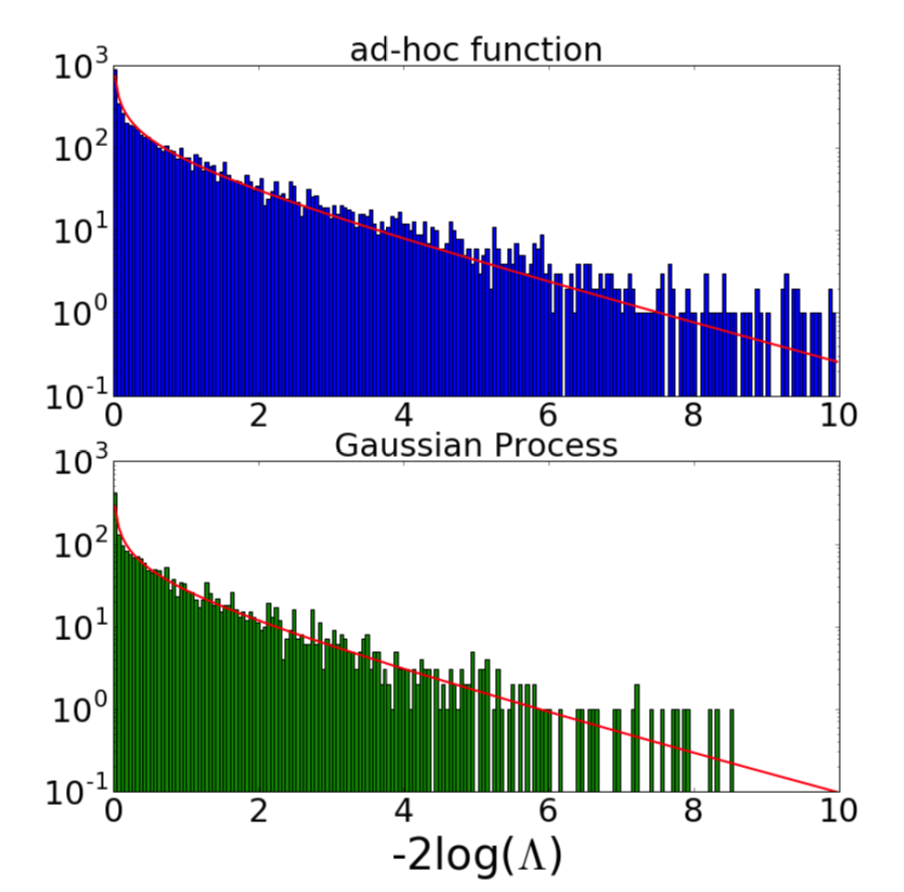
\includegraphics[width=0.75\textwidth]{figures/chapter_analysismethod/chi2}
                \caption{
                This figure shows the negative log of the $\Lambda$ which is an approximation of the measure of the profiled likelihood ratio defined in~\ref{eq:profilelikelihood}. The top part is the distribution for background only pseudo-experiments, whereas the bottom is the background + signal distribution. They show a reasonable agreement to the $\chi^{2}$ fit, a required condition for the Asimov approximation for a frequentist limit setting~\cite{frate2017modeling}. 
            }
            \label{fig:chi2}
        \end{center}
    \end{figure}
    \FloatBarrier

    A new test statistic for Gaussian Process that is parametrized by the kernel hyper-parameters is used instead for limit setting:

\begin{equation}
    -ln(\Lambda) \textrm{, where }\Lambda= 2ln(\frac{L_{\textrm{GP signal + bkg fit}}(\mu, \hat{\hat{\theta}})}{L_{\textrm{GP bkg fit}}(\hat{\mu}, \hat{\theta})})
\end{equation}

Here, $\ln(\Lambda)$ is the new test statisitics used for the limit setting L is the likelihood defined in Eq.~\ref{eq:loglikelihood}. The numerator is the likelihood with both the background and signal kernel, whereas the denominator is likelihood with just the background kernel. 

With the above procedure in place, actual data from analysis is ready to be analyzed for resonance in the dijetISR and dimuon channels.

 
%
\chapter{The Search for the Resolved Dijet ISR Signature}
\label{chapter:dijet}

Disclaimer:
This chapter is taken from the paper of \cite{2019} directly.
The full ATLAS author list can be found there. The individual author contribution including my own can be found in the end of the chapter.

%\include{ANA-EXOT-2018-05-PAPER/ANA-EXOT-2018-05-PAPER.tex}

%-------------------------------------------------------------------------------
\section{Introduction}
%% \label{sec:intro}
%-------------------------------------------------------------------------------

\let\oldTeV\TeV
\let\oldGeV\GeV
\renewcommand{\TeV}{\oldTeV\xspace}
\renewcommand{\GeV}{\oldGeV\xspace}

% \newcommand{\ZprimeLimitStatement}{for masses $m_{\Zprime}$ of 250~\GeV and $\approx$400--550~\GeV, for couplings values of $\gq\sim 0.3$ and larger}
%\newcommand{\PhotonGaussianLimitStatement}{from approximately 340~fb at a mean mass of 250~\GeV to approximately 6~fb at 1.2~\TeV}
\newcommand{\PhotonGaussianLimitStatement}{from approximately 100--150~fb at a mean mass of 200~\GeV to approximately 10--20~fb at 1.2~\TeV}
\newcommand{\JetGaussianLimitStatement}{from approximately 100~fb at a mean mass of 350~\GeV to approximately 50~fb at 550~\GeV}
\newcommand{\JetZprimeLimitStatement}{\textbf{To be updated} for $\gq$ above 0.20 at mass $m_{\Zprime}=350$~\GeV and $\gq$ above 0.22 at $m_{\Zprime}=550$~\GeV}

Searches for resonant enhancements of the dijet invariant mass distribution (\mjj) are an essential part of the LHC physics programme.
%New particles produced directly in LHC collisions must interact with the constituent partons of the proton, and they may also decay to partons in the final state.
New particles with sizeable couplings to quarks and gluons are predicted by many models, such as those including resonances with additional couplings to dark-matter particles~\cite{Chala:2015ama,LHCDMF:2015}.

Searches for dijet resonances with masses of several hundreds of \GeV to just above 1~\TeV have been carried out at lower-energy colliders~\cite{Arnison:1983dk,Albajar:1988rs,Bagnaia1984283, Aaltonen:2008dn,Alitti:1990kw} and at the LHC, which has also extended search sensitivities into the multi-$\TeV$ mass range~\cite{EXOT-2010-01,CMS-EXO-10-010,CMS-QCD-10-016,CMS-EXO-11-015,EXOT-2010-07,EXOT-2011-07,EXOT-2011-21,EXOT-2013-11,CMS-EXO-12-016,EXOT-2015-02,CMS-EXO-13-001,CMS-EXO-16-056,CMS-EXO-16-032,EXOT-2016-20,EXOT-2016-21}.
Despite using higher integrated luminosities than earlier colliders, these LHC searches have been limited at lower masses by a large multi-jet background. 
Multi-jet events are produced at such high rates that fully recording every event would saturate the online data selection (called \textit{trigger}) and data acquisition systems.
To avoid this, minimum transverse momentum ($\ptmin$) thresholds are imposed on triggers collecting events with at least one jet (called single-jet triggers).
These thresholds create a lower bound on the sensitivity of searches 
%using these triggers 
at a mass of approximately $\mjj \approx 2\ptmin$, where $\ptmin$ is typically several hundred $\GeV.$
Consequently, searches for dijet resonances at the LHC have poor sensitivity for masses below $1\,\TeV$, and set limits on the couplings of the resonance to quarks in this light-resonance region which are weaker than limits in heavy-resonance regions~\cite{Dobrescu:2013coa}.
Nevertheless, despite the difficulty of recording events containing light resonances, they remain a viable search target at the LHC, both from a model-agnostic point of view~\cite{Harris:2011bh} and, for example, in models of spin-dependent interactions of quarks with dark matter~\cite{Chala:2015ama,LHCDMF:2015}. 

Recently, ATLAS and CMS have published searches for low-mass dijet resonances using several complementary strategies to avoid trigger limitations.
For $\mjj~>~450\,\GeV$, the most stringent limits are set by searches recording only partial event information~\cite{CMS-EXO-16-032,EXOT-2016-20}.

Another search avenue is opened by data in which a light resonance is boosted in the transverse direction via recoil against a high-$\pt$ photon~\cite{An:2012ue,Shimmin:2016vlc}.
Requiring a high-\pT photon in the final state reduces signal acceptance but allows efficient recording of events with lower dijet masses.
At even lower resonance masses, the decay products of the resonance will merge into a single large-radius jet. 
Searches for this event signature have been used to set limits on resonant dijet production at both ATLAS~\cite{EXOT-2017-01} and CMS~\cite{CMS-EXO-17-001,Sirunyan:2018ikr}.
However, these searches become less sensitive above $200\,\GeV$--$350\,\GeV$, when the decay products fall outside the large-radius jet cone.
%% btagged: EXOT-2016-33, goes to 0.57 TeV
%% TLA: EXOT-2016-20, goes to 0.45 TeV
%% Boosted: EXO-17-001, goes up to 0.22 TeV

This Letter presents a new search for resonances in events containing a dijet and a high-\pT photon in the final state, using proton--proton ($pp$) collisions recorded at a centre-of-mass energy $\sqrt{s} =$ 13~\TeV and corresponding to an integrated luminosity up to 79.8~\ifb.
The search targets a dijet mass range of \ApproxMassRangeGamma.
This range covers masses below the range accessible using single-jet triggers or partial-event data and above the mass range where the resonance decay products merge.
The search is performed using samples of events selected either with or without criteria designed to identify jets originating from bottom quarks (\textit{$b$-jets}).
Searching in a subset of the data selected with $b$-jet identification criteria enhances sensitivity to resonances which preferentially decay into bottom quarks.
This search probes masses above $225\,\GeV$, obtaining results complementary to the reach of previous dijet searches at a centre-of-mass energy of $\sqrt{s} =$ 13~\TeV: below approximately $600\,\GeV$, previous ATLAS di-$b$-jet searches lose sensitivity~\cite{EXOT-2016-33}, while the range of the CMS boosted di-$b$-jet search~\cite{Sirunyan:2018ikr} is limited to a mass region up to 350~\GeV. Another complementary CMS search for resonances with masses above $325\,\GeV$ decaying to $b$-jets at a centre-of-mass energy of $\sqrt{s} =$ 8~\TeV is described in Ref.~\cite{CMS-EXO-16-057}.

%% A complementary search, recording only partial event data in order to efficiently trigger on dijet events without requiring an ISR object, has been performed also focusing on light resonances with dijet masses of 425~\GeV--1.05~\TeV~in ATLAS~\cite{tla} and with dijet masses of 450~\GeV--1.6~\TeV~in CMS~\cite{Khachatryan:2016ecr}. Another recent complementary search for resonances with masses of 600~\GeV and above decaying to heavy-flavour jets is described in Ref.~\cite{lowMassDiB}.

%-------------------------------------------------------------------------------
\section{ATLAS detector}
%% \label{sec:detector}
%-------------------------------------------------------------------------------


%\newcommand{\AtlasCoordFootnote}{%
%ATLAS uses a right-handed coordinate system with its origin at the nominal interaction point (IP) in the centre of the detector and the $z$-axis along the beam pipe.
%The $x$-axis points from the IP to the centre of the LHC ring, and the $y$-axis points upwards.
%Cylindrical coordinates $(r,\phi)$ are used in the transverse plane, with $\phi$ being the azimuthal angle around the $z$-axis.
%The pseudorapidity is defined in terms of the polar angle $\theta$ as $\eta = -\ln \tan(\theta/2)$.
%It is equivalent to the rapidity for massless particles. 
%Transverse momentum and energy are defined as $\pt\equiv p \sin{\theta}$ and $\ET\equiv E \sin{\theta}$, respectively.
%Angular distance is measured in units of $\Delta R \equiv \sqrt{(\Delta\eta)^{2} + (\Delta\phi)^{2}}$.}
%
%The ATLAS experiment~\cite{PERF-2007-01,Capeans:1291633,CERN-LHCC-2012-009,Abbott:2018ikt} at the LHC is a multipurpose particle detector with a forward--backward symmetric cylindrical geometry\footnote{\AtlasCoordFootnote\xspace} with layers of tracking, calorimeter, and muon detectors over nearly the entire solid angle around the $pp$ collision point.
%The directions and energies of high transverse momentum particles are measured using tracking detectors, finely segmented hadronic and electromagnetic calorimeters, and a muon spectrometer, within axial and toroidal magnetic fields.
%The inner tracker consists of silicon pixel, silicon microstrip, and transition radiation tracking detectors, and reconstructs charged-particle tracks in $|\eta| < 2.5$.
%Lead/liquid-argon (LAr) sampling calorimeters provide electromagnetic (EM) energy measurements with high granularity.
%A steel/scintillator-tile hadronic calorimeter covers the central pseudorapidity range ($|\eta| < 1.7$).
%The endcap and forward regions are instrumented with LAr calorimeters for EM and hadronic energy measurements up to $|\eta| = 4.9$.
%The trigger system~\cite{TRIG-2016-01} consists of a first-level trigger implemented in hardware, using a subset of the detector information to reduce the accepted rate to 100 kHz, followed by a software-based trigger that reduces the rate of recorded events to about 1 kHz.
%
%-------------------------------------------------------------------------------
\section{Data samples and event selection}
%% \label{sec:analysis}
%-------------------------------------------------------------------------------

%% You can find some text snippets that can be used in papers in \texttt{template/atlas-snippets.tex}.
%% Some of the snippets need the \texttt{jetetmiss} option passed to \texttt{atlasphysics}.
%% %\input{atlas-snippets}

The result presented in this Letter is based on data collected in $pp$ collisions at $\sqrt{s} = 13\,\TeV$ during 2015--2017.
The signal consists of events with two jets from the decay of a new particle, and an additional photon, radiated off one of the colliding partons.

Data were collected via either a single-photon trigger or a combined trigger requiring additional jets, to allow a lower \pT requirement on the photon. 
The data collected with the single-photon trigger are used to search for resonances with masses from 225 GeV to 450 GeV, while the data collected with the combined trigger are used to search for resonances with masses from 450 GeV to 1.1 TeV.  

The single-photon trigger requires at least one photon candidate with $\photonPtTrig > 140\,\GeV$, where $\photonPtTrig$
is the photon transverse energy as reconstructed by the software-based trigger.
The combined trigger requires a photon and two additional jet candidates, each with $\pt > 50\,\GeV$.
The combined trigger requires $\photonPtTrig > 75\,\GeV$ for the 2016 data, increasing to $\photonPtTrig > 85\,\GeV$ for the 2017 data.
This trigger was not active during the 2015 data-taking period.
As a consequence, the single-photon trigger recorded $79.8\,\ifb$ of data and the combined trigger recorded $76.6\,\ifb$ of data.
Both triggers are fully efficient within uncertainties in the kinematic regimes used for this analysis.

After recording the data, a subset of collision events consistent with the signal are selected to populate $\mjj$ distributions for subsequent analysis.
A brief description of the reconstruction methods is given below together with the event selection.

In all of the events selected for analysis, all components of the detector are required to be operating correctly. 
In addition, all events are required to have a reconstructed primary vertex~\cite{ATLAS-CONF-2014-018}, defined as a vertex with at least two reconstructed tracks, each with $\pT > 500~\MeV$. 

Photon candidates are reconstructed from clusters of energy deposits in the electromagnetic calorimeter~\cite{PERF-2017-02}.
The energy of the candidate is corrected by applying energy scale factors measured with $Z \rightarrow e^+e^-$ decays~\cite{PERF-2013-05}.

The trajectory of the photon is reconstructed using the longitudinal segmentation of the calorimeters along the shower axis (shower depth) and a constraint from the average collision point of the proton beams.
Candidates are restricted to the region $|\eta| < 2.37$, excluding the transition region $1.37 < |\eta| < 1.52$ between the barrel and endcap calorimeters to ensure that they arise from well-calibrated regions of the calorimeter. An additional requirement is applied on the transverse energy of the photon candidate after reconstruction, which is required to have $\photonPt > 95\,\GeV$, where $\photonPt$ is the  transverse energy of the photon candidate after reconstruction.
%These requirements ensure the candidates arise from well-calibrated regions of the calorimeter.
%and have an energy above the thresholds of the two triggers required.

Quality requirements are applied to the photon candidates to reject events containing misreconstructed photons arising from instrumental problems or from non-collision backgrounds.
Further \emph{tight} identification requirements are applied to reduce contamination from $\pi^0$ or other neutral hadrons decaying into two photons~\cite{PERF-2017-02}.
The photon identification is based on the profile of the energy deposits in the first and second layers of the electromagnetic calorimeter.
In addition to the tight identification requirement, candidates must meet \emph{tight isolation} criteria using calorimeter and tracking information, requiring that they be separated from nearby event activity~\cite{PERF-2017-03,HIGG-2016-17}.
%% The transverse energy deposited in the calorimeters in a cone of size $\Delta R = 0.4$ around the cluster barycentre, excluding the energy associated with the photon cluster, is required to be less than $2.45~\textrm{GeV} + 0.022 \times \photonPt$.
%% The energy in the cone is corrected for the leakage of the photon energy from the central core and for the effects of additional $pp$ interactions occurring within the same and neighbouring bunch crossings (pile-up)~\cite{PERF-2017-03,Aad:2010sp}.
%% Additionally, the scalar sum of transverse momentum of tracks measured by the inner tracker in a cone $\Delta R = 0.2$ around the candidate must be less than $0.05 \times \photonPt$.
%% The photon candidates without matching tracks in the inner tracking detector are classified as \emph{unconverted} photon candidates.
%Photons may interact with detector material, producing one or more charged-particle tracks and failing to meet the photon isolation criteria.
%To recover these events, \emph{converted} 
Converted photon candidates matched to one track or a pair of tracks passing inner-detector quality requirements~\cite{PERF-2017-02} and satisfying tight identification and isolation criteria are also considered.
Any pair of matching tracks must form a vertex that is consistent with originating from a massless particle.
%% The position of this conversion vertex is used when computing the photon trajectory if tracks from the conversion have hits in the silicon detectors. 
%% A single-track photon candidate must include tracking measurements in the TRT and at least one measurement in the silicon detector after the innermost layer of the pixel detector.
%% The criteria for unconverted candidates to be isolated from nearby event activity must also be satisfied by converted candidates.
% Tracks participating in the converted photon candidate are not included in the isolation calculation.
%These photon requirements are satisfied by approximately 83\% and 97\% of the events produced by a typical new physics resonant signal as described below, with a mass of 250 GeV and a coupling to quarks of 0.2.

Jets are reconstructed using the anti-$k_{t}$ algorithm~\cite{antikT,Cacciari:2006} with radius parameter $R = 0.4$ from clusters of energy deposits in the calorimeters~\cite{PERF-2014-07}.
Quality requirements are applied to remove events containing spurious jets from detector noise and out-of-time energy deposits in the calorimeter from cosmic rays or other non-collision sources~\cite{ATLAS-CONF-2015-029}.
Jet energies are calibrated to the scale of the constituent particles of the jet and corrected for the presence of multiple simultaneous (pile-up) interactions~\cite{PERF-2014-03,PERF-2016-04}.

After reconstruction, jets with transverse momentum $\jetPt > 25\,\GeV$ and rapidity $|\jetEta| < 2.8$ are considered.
To suppress pile-up contributions, jets with $\jetPt < 60\,\GeV$ and $|\jetEta|<2.4$ 
are required to originate from the primary interaction vertex with the highest summed $\pT^2$ of associated tracks.
If a jet and a photon candidate are within $\Delta R = 0.4$, the jet candidate is removed.

These requirements retain approximately 30\% of a typical signal sample. 

Jets which likely contain $b$-hadrons are identified (\btagged) with the \textsc{DL1} flavour tagger~\cite{ATL-PHYS-PUB-2017-013}.
Tracks are selected in a cone around the jet axis, using a radius which shrinks with increasing \jetPt.
The selected tracks are used as input to algorithms which attempt to reconstruct a $b$-hadron decay chain.
The resulting information is passed to a neural network which assigns a $b$-jet probability to each jet.
To account for mismodelling in simulated $b$-hadron decays, a comparison of the discrimination power of this network in data and Monte Carlo simulation is performed and correction factors are applied to simulation to reproduce the data~\cite{PERF-2016-05}.
Jets are considered \btagged when the \textsc{DL1} score exceeds a threshold consistent with a 77\% $b$-hadron identification efficiency on a benchmark $t \bar{t}$ sample. At this threshold, only 0.7\% light-flavour jets and 25\% charm-jets are retained.

Events which contain at least one photon candidate and two jets are selected using the above criteria
and separated into four categories for further analysis. 
Two of the categories are constructed with flavour-inclusive criteria, for which \btagging\ results are ignored.
One of these two categories contains events recorded via the single-photon trigger, and the other category contains events recorded via the combined trigger.
To ensure the trigger is fully efficient, events in the single-photon-trigger category are required to have a photon with $\photonPt >150\,\GeV$ and events in the combined-trigger category are required to have a photon with $\photonPt > 95\,\GeV$ and two jets with $\jetPt > 65\,\GeV$.
The remaining two categories consist of events selected as in the flavour-inclusive categories, except that the two highest-\jetPt jets must satisfy the $b$-tagging criteria and have $|\jetEta| < 2.5$ to ensure that they fall within the acceptance of the tracking detectors.

Dijet production at the LHC occurs largely via $t$-channel processes, leading to jet pairs with high absolute values of $\yStar = (y_1-y_2)/2$, where $y_1$ and $y_2$ are the rapidities of the highest-\pT\ (leading) and second-highest-\pT\ (subleading) jet, respectively.
On the other hand, heavy particles tend to decay more isotropically, with the two jets having lower $|\yStar|$ values.
Therefore, $|y^*| < 0.75$ is required for all four categories.
This selection rejects up to 80\% of the multi-jet background events while accepting up to 80\% of the signal events discussed below.
A further selection is applied to select events above a given invariant mass depending on the trigger, $\mjj > 169~\GeV$ for the single-photon trigger and $\mjj > 335~\GeV$ for the combined trigger.
This is so that the background can be described by a smoothly falling analytic function satisfying the goodness-of-fit criteria described in~\ref{sec:background}.

%%%%%%%%%%%%%%%%%%%%%%%
%% Cut definition
%
%
\begin{table}[!h]
\setlength{\tabcolsep}{10pt}
	\centering
	\caption[]{Event selections used to construct each of the four event categories, as described in the text.}
        \begin{tabular}{ l c c c c}
                \toprule
                 Criterion & Single-photon trigger & Combined trigger \\
                 \midrule
                        Number of jets & \multicolumn{2}{c}{$\njet \geq 2$} \\ 
                        Number of photons & \multicolumn{2}{c}{$\nphoton \geq 1$} \\
                        Leading photon & $\photonPt > 150~\GeV$ & $\photonPt >  95~\GeV$ \\
                        Leading, subleading jet & $\jetPt > 25~\GeV$ & $\jetPt> 65~\GeV$ \\
                        Centrality & \multicolumn{2}{c}{$|\yStar|=|y_{1} - y_{2}|/2 < 0.75$}  \\
                        Invariant mass & $\mjj > 169~\GeV$ & $\mjj > 335~\GeV$ \\
                \midrule
                \midrule
                        Criterion (applied to each trigger selection) & Inclusive & $b$-tagged \\
                \midrule
                        Jet $|\eta|$ & $|\jetEta| < 2.8$ & $|\jetEta| < 2.5$ \\
                        $b$-tagging & -- & $\ntag\geq 2$ \\
                \bottomrule
        \end{tabular}   
    %Events are collected using a single-photon trigger for low dijet masses and collected with a multi-object ``combined'' trigger for high dijet masses.
    %These two categories are further subdivided into flavour-inclusive categories and categories requiring that the two leading jets pass \btagging\  requirements (defined by the 77\% fixed efficiency working point of the ATLAS DL1 tagger).
    %All jets in the analysis are required to fall within $|\eta| < 2.8$.
    %For the \btagged selections, the two highest-\pt jets must lie within the tracker acceptance, $|\eta| < 2.5$.
        \label{tab:analysisselection}
\end{table}

The above selections, summarised in Table~\ref{tab:analysisselection}, yield 2,522,549 and 15,557 events acquired by the single-photon trigger for the flavour-inclusive and \btagged categories, respectively. 
They yield 1,520,114 and 9,015 events acquired by the combined trigger in the corresponding categories.

The distributions of $\mjj$ for events in each of the four categories are shown in Fig.~\ref{fig:data}.
Hypothetical signals with $m_{\Zprime}= 250\,\GeV$ and $m_{\Zprime}= 550\,\GeV$, as further discussed in Section~\ref{sec:limits}, are overlaid.

At the largest dijet masses considered, the combined-trigger categories provide greater sensitivity to signals than the single-photon-trigger categories due to their greater signal acceptance. The sensitivity is defined as $S/\sqrt{B}$, where $S$ and $B$ are the number of signal and background events in the simulation samples described in Section~\ref{sec:limits}. 
At the smallest dijet masses considered, the jet $\pT$ thresholds of the combined trigger cause those categories to lose efficiency for signals and bias the $\mjj$ distributions of the background processes.
Therefore, to optimise the search across a wide range of signal masses, the invariant mass spectra selected using the combined-trigger categories are used in the search for signal masses above $450\,\GeV$, while the spectra obtained with the single-photon trigger are used for lower masses.

\section{Background estimation}
\label{sec:background}

To estimate the Standard Model contributions to the distributions in Fig.~\ref{fig:data}, smooth functions are fit to the data.
The dijet searches of the CDF, CMS, and ATLAS experiments~\cite{Aaltonen:2008dn,EXOT-2010-01,CMS-EXO-11-015,EXOT-2013-11,EXOT-2015-02,EXOT-2015-02,EXOT-2013-11,Alitti:1990kw,CMS-EXO-16-032} have successfully modelled dijet mass distributions in hadron colliders using a single function over the entire mass range considered in those searches.
This approach is not suitable when data constrain the fit too tightly for a single function to reliably model both ends of the distribution simultaneously.
Here, a more flexible technique is adopted, similar to that used in recent ATLAS dijet resonance searches~\cite{EXOT-2016-21,EXOT-2016-20}. 
In this technique, a single fit using a given function over the entire mass distribution is replaced by many successive fits.
For each bin of the mass distribution, the same function is used to fit a broad mass range centred on the bin, and the background prediction for that bin is taken to be the value of the fitted function in the centre of the range.
The process is repeated for each bin of the mass distribution and the results are combined to form a background prediction covering the entire distribution. For invariant masses higher than the \mjj\ range used for the search (above 1.1 TeV), the window is allowed to extend beyond the range as long as data is available.

A set of parametric functions are considered for these fits:%\footnote{\textcolor{red}{NOTE: The UA2 function is never used, we could avoid discussing it here? Or keep to demonstrate the difficulty of alternative modeling?}}:

\begin{equation}
f(x) = p_1 x^{-p_2} \mathrm{e}^{-  p_3  x - p_4  x^2}
\label{eq:ua2}
\end{equation}

or 

\begin{equation}
f(x) = p_1 (1 - x)^{p_2} x^{p_3 + p_4\ln x  + p_5(\ln x)^2} \label{eq:5par},
\end{equation}

\noindent
where $x = \mjj/\sqrt{s}$ and $p_i$ are free parameters determined by fitting the $\mjj$ distribution.
In addition to the five-parameter function in Eq.~(\ref{eq:5par}), a four-parameter variant with $p_5 = 0$ and a three-parameter variant with $p_5 = p_4 = 0$ are also considered.
The width of the mass range used for the individual fits was optimised to retain the broadest possible range while maintaining a $\chi^2$ $p$-value above 0.05 in regions of the distribution that do not contain narrow excesses, where excesses are identified using the \BumpHunter algorithm described in the next section. 
The sliding window procedure cannot be extended beyond the lower edge of the \mjj range used in each signal selection. 
Therefore, until the optimal number of bins is reached on each side of a given bin center, the start of the window is fixed to the lower edge of the spectrum and the fitted functional form is evaluated for each bin in turn. 
This procedure allows for a stable background estimate while maintaining sensitivity to signals localised in the \mjj distribution. 
Tests performed by adding sample signals to smooth pseudo-data distributions confirmed that this approach can find signals of width-to-mass ratios up to 15\%, with sensitivity increasing for narrower signals.  The ranges of the individual fits vary from 750~\GeV in the narrowest case to 1600~\GeV in the widest case. A signal with a 15\% width-to-mass ratio constrained by the narrowest fit would have an absolute width of 163~\GeV, or less than one quarter of the fit range.
 
%% Samples of simulated events are used to characterise the hypothetical resonances as well as to study the kinematic distributions of background processes. However, these samples are not used to estimate the background contributions, except to validate the data-driven background estimation procedure (described in Sec.~\ref{sec:background}).
Monte Carlo samples of background containing a photon with associated jets were simulated using \textsc{Sherpa}~2.1.1 \cite{Gleisberg:2008ta}, generated in several bins of photon transverse momentum at the particle level (termed as $\photonPt$ for this paragraph), from 35~\GeV up to energies where backgrounds become negligible in data, at approximately 4~\TeV.
The matrix elements, calculated at next-to-leading order (NLO) with up to three partons for  $\photonPt<70$~\GeV or four partons for higher $\photonPt$,
were merged with the \textsc{Sherpa} parton shower~\cite{Schumann:2007mg} using the \textsc{ME+PS@LO} prescription~\cite{Hoeche:2009rj}.
The \textsc{CT10} set of parton distribution functions (PDF)~\cite{Lai:2010vv} was used in conjunction with the dedicated parton shower tuning developed by the \textsc{Sherpa} authors.
These samples, alone and in combination with the signal samples discussed below, were used to validate the background model obtained with the above mentioned method, and they were also used to verify that the fitting procedure is robust against false positive signals. Additionally, the simulated samples were used to calculate the fractional dijet mass resolution, which was found to be in the range 8\%--3\% for the masses of 225~\GeV up to 1.1~\TeV considered in this search.

% This ansatz also describes the {\textsc Sherpa} simulation of Standard Model processes that yield a jet pair and ISR photon and high-statistics \PYTHIA simulations of three-jet events, described above. A log-likelihood-ratio statistic employing Wilks's theorem~\cite{wilks1938} was used to determine if the background estimation would be significantly improved by an additional degree of freedom.

%% With the current dataset and using the same criteria as Ref.~\cite{}, Eq.~\ref{func} was found to be sufficient for the $X+\gamma$ analysis. Eq.~\ref{func} with $c_4$ set to zero was found to be sufficient for $X+j$ search. The lower bound of the fit range, \FitStartGamma for the $X+\gamma$ search and \FitStartJet for the $X+j$ search, is chosen to exclude kinematic bias from the $\pt$ requirement of the photon and jet trigger, respectively. The fit is performed on the binned data, with varying bin widths proportional to the detector $\mjj$ resolution, which varies from approximately 6\% at $\mjj=250$~\GeV to 2.7\% at $\mjj=1.5$~\TeV.

\begin{figure}
  \centering
  \begin{subfigure}[b]{0.49\textwidth}
    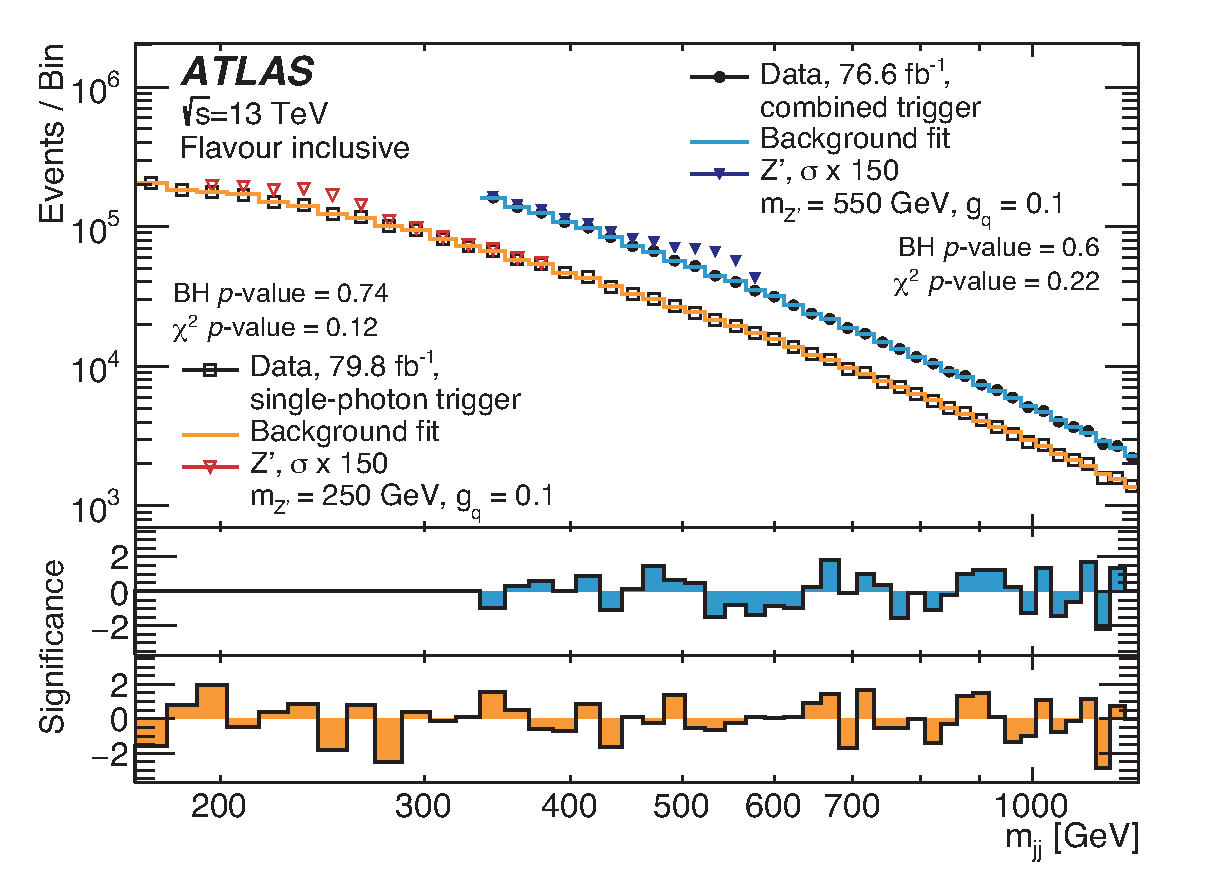
\includegraphics[width=\textwidth]{figures/ISR_resolved/figure1_inclusive_withTrigLabels_noBumpLimits}
    \caption{\label{fig:1a}}
  \end{subfigure}
  \begin{subfigure}[b]{0.49\textwidth}
    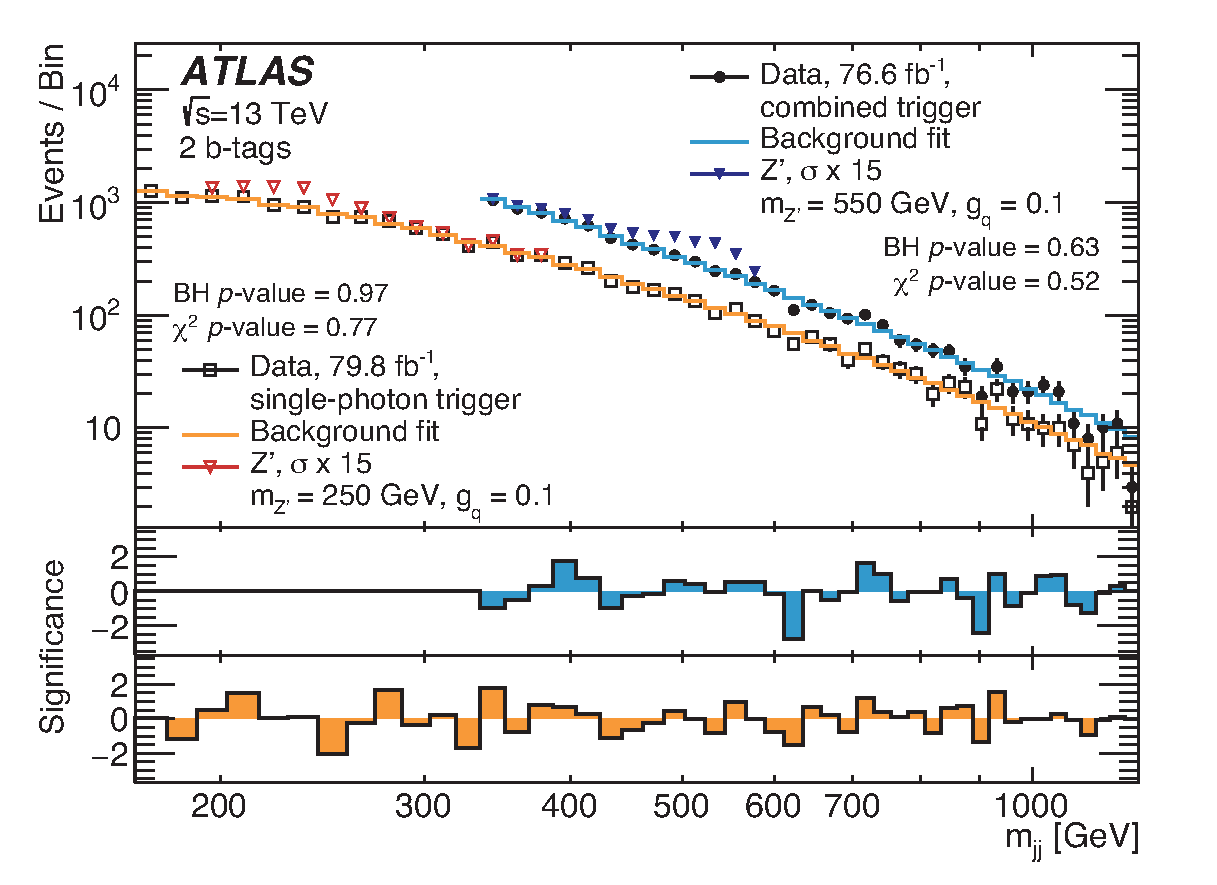
\includegraphics[width=\textwidth]{figures/ISR_resolved/figure1_nbtag2_withTrigLabels_noBumpLimits}
    \caption{\label{fig:1b}}
  \end{subfigure}
  \caption[]{Dijet mass distributions for the \subref{fig:1a} flavour-inclusive and \subref{fig:1b} \btagged categories.
  In both figures, the distribution for the sample collected using the combined trigger with $\photonPt > 95\,\GeV$ and two $\jetPt > 25\,\GeV$ jets (filled circles) and the distribution for the sample collected using the single-photon trigger with $\photonPt > 150\,\GeV$  (open squares) are shown separately. 
  The solid lines indicate the background estimated from the fitting method described in the text.
%    For the flavour-inclusive distributions, the method uses the 5 parameter variant of Eq.~(\ref{eq:5par}) in the single-photon triggered case and the 4 parameter variant of Eq.~(\ref{eq:5par}) in the combined trigger case.
%    In the \btagged categories, the method uses the 4 parameter variant of Eq.~(\ref{eq:5par}) in the single-photon triggered case and the 3 parameter variant of Eq.~(\ref{eq:5par}) in the combined trigger case.
    Also shown are 
    %the most-discrepant mass interval identified by \BumpHunter\ (dashed vertical lines) and 
    the $p$-values  both by a $\chi^2$ comparison of data to background estimate and by \BumpHunter (BH). 
    The solid and empty triangles represent a $\Zprime$ injected signal with \gq = 0.1, masses of 550 and 250~\GeV, respectively, where the theory-cross section is multiplied by the factor shown in the legend.
    The bottom panels show the significances of bin-by-bin differences between the data and the fits for the combined trigger (middle) and single-photon trigger (bottom).
    These Gaussian significances are calculated from the Poisson probability, considering only statistical uncertainties on the data.
  }
  \label{fig:data}
\end{figure}


\section{Search results}
\label{sec:result}
%-------------------------------------------------------------------------------

Fig.~\ref{fig:data} shows the results of fitting each of the observed distributions, as described in Section~\ref{sec:background}.
For each distribution, the function among those in Eqs.~(\ref{eq:ua2}) and (\ref{eq:5par}) and their variants which yields the highest $\chi^2$ $p$-value (shown in the figure), in absence of localized excesses, is chosen as the primary function for the fitting method.
The function with the lowest $\chi^2$ $p$-value which still results in a $p$-value larger than 0.05 is chosen as an alternative function.
The primary and alternative functions for each of the four search categories are shown in Table~\ref{tab:fitsummary}.
The alternative function is used to estimate the systematic uncertainty of the background prediction due to the choice of function, as described below.

%%%%%%%%%%%%%%%%%%%%%%
% Summary of fit functions

\begin{table}
  \caption[]{Summary of functions used for background fits to each category.
    The five-parameter function (5~par.) is given in Eq.~(\ref{eq:5par}).
    The four-parameter variant (4~par.) sets $p_5 = 0$, while the three-parameter variant (3~par) sets $p_5 = p_4 = 0$.}
    %The UA2 function is given by Eq.~(\ref{eq:ua2}). 
  \begin{tabularx}{\textwidth}{ l | *4{>{\centering\arraybackslash}X}@{}}
    \toprule
    \centering
		Fit               						        & Flavour-inclusive, single~$\gamma$~trigger     & Flavour-inclusive, combined~trigger 			& \btagged, single~$\gamma$~trigger   		   & \btagged, combined~trigger.        \\ \midrule
        Primary fit 								    & Eq.~(\ref{eq:5par}), 5~par.   & Eq.~(\ref{eq:5par}), 4~par. & Eq.~(\ref{eq:5par}), 4~par. & Eq.~(\ref{eq:5par}), 3~par. \\
        ($\chi^2$ $p$-value)       						& (0.11) 					    & (0.23)  					  &  (0.75)  				    & (0.53) 					  \\ \midrule
        Alternative fit 							    & Eq.~(\ref{eq:5par}), 4~par.	& Eq.~(\ref{eq:ua2}) 		  & Eq.~(\ref{eq:5par}), 3~par. & Eq.~(\ref{eq:5par}), 5~par.\\ 
 	    ($\chi^2$ $p$-value)       						& (0.07) 					    & (0.20)  					  &  (0.75)  				    & (0.44) 					  \\ \bottomrule
 	\end{tabularx}
    \label{tab:fitsummary}
\end{table}

%% In all cases the fits agree with the observed data with a  $p$-value above $0.5$.
%% The lower panels of the figure show the significances of bin-by-bin differences between the data and the fits. These Gaussian significances are calculated from the Poisson probability considering only statistical uncertainties. The data have been overlaid with examples of the signals described in Sec.~\ref{sec:samples}.
The statistical significance of any localised excess in each $\mjj$ distribution is quantified using the \BumpHunter~(BH) algorithm~\cite{Aaltonen:2008vt,Choudalakis:2011bh}.
The algorithm compares the binned $\mjj$ distribution of the data with the fitted background estimate, considering mass intervals centered in each bin location and with widths of variable size from two bins up to half the mass range used for the search (169 or 335 GeV to 1.1 TeV, for the single and combined trigger respectively). 
%In Figure~\ref{fig:data}, the region labelled \emph{\BumpHunter\ interval} depicts the most discrepant interval found for each distribution.

The statistical significance of the outcome is evaluated using the ensemble of possible outcomes by applying the algorithm to many pseudo-data samples drawn randomly from the background fit.
Without including systematic uncertainties, the \BumpHunter\ $p$-value -- the probability that fluctuations of the background model would produce an excess at least as significant as the one observed in the data, anywhere in the distribution -- is $p > 0.5$ for all distributions.
Thus, there is no evidence of a localised contribution to the mass distribution from new phenomena.

\section{Limit setting}
\label{sec:limits}

Limits are set on the possible contributions to the $\mjj$ distributions from two kinds of resonant signal processes.
As a specific benchmark signal, a leptophobic $\Zprime$ resonance is simulated as in Refs.~\cite{LHCDMF:2015,EXOT-2015-02}.
The $\Zprime$ resonance has axial-vector couplings to quarks and to a fermion dark-matter candidate.
The coupling of the $\Zprime$ to quarks, $\gq$, is set to be universal in quark flavour.
The mass of the dark-matter fermion is set to a value much heavier than the $\Zprime$, such that the decay width to dark matter is zero.
The total width $\Gamma_{\Zprime}$ is computed as the minimum width allowed given the coupling and mass $m_{\Zprime}$; this width is $3.6\%$--$4.2\%$ of the mass for $m_{\Zprime}=0.25$--$0.95$~\TeV and $\gq=0.3$. 
The interference between the $\Zprime$ in this benchmark model and the Standard Model $Z$ boson is assumed to be negligible.
A set of event samples were generated at leading order with $m_{\Zprime}$ values in the range 0.25--1.5~\TeV and with $\gq=0.3$ using \MGMCatNLOV{2.2.3}~\cite{Alwall:2014hca}; the \textsc{NNPDF3.0 LO} PDF set~\cite{Ball:2012cx} was used in conjunction with \PYTHIA~8.186~\cite{Sjostrand:2007gs} and the \textsc{A14} set of tuned parameters~\cite{ATL-PHYS-PUB-2014-021}.
For these samples, the acceptances of the kinematic selections in the flavour-inclusive categories range from 1\% to 2.5\%, increasing with signal mass, for the sample collected by the combined trigger and from 4\% to 10\% for the sample collected by the single-photon trigger. 
For the \btagged categories, the kinematic acceptance is defined relative to the full flavour-inclusive generated samples, leading to acceptance values of 0.2\%--0.4\% and 0.7\%--1.6\% for the combined and single-photon trigger, respectively. 
The reconstruction efficiencies range from 74\% to 80\% for the flavour-inclusive categories and from 40\% to 48\% for the \btagged categories, decreasing with increasing signal mass.

%In each search, a Bayesian method with a constant prior is applied to the $\mjj$ data and simulation of signals for discrete mass values to set 95\% credibility-level (CL) upper limits on the cross-section times acceptance for the signals described above~\cite{EXOT-2010-07}.
Limits are set on the considered new-physics contributions to the $\mjj$ distributions using a Bayesian method. 
A constant prior is used for the signal cross-section and Gaussian priors for nuisance parameters corresponding to systematic uncertainties. 
The expected limits are calculated using pseudo-experiments generated from the background-only component of a signal-plus-background fit to the data, using the same fitting ranges and functions selected as the best model in the search phase.  
Signal hypotheses at discrete mass values are used to set 95\% credibility-level (CL) upper limits on the cross-section times acceptance ~\cite{EXOT-2010-07}.
The limits are obtained for a discrete set of points in the $\gq$--$m_{\Zprime}$ plane, shown in Fig.~\ref{fig:limits_zprime}. 
 %% The signal mass range probed by the $X+\gamma$ search ranges from 250 GeV to 950 GeV, while the mass range for the  $X+j$ search spans 350 to 550 GeV. In both searches, the choice of mass points ensures that the presence of signal does not bias the background estimation. In the case of the $X+j$ search, the sensitivity to signal masses above 550 GeV is reduced by the increasing number of events where the subleading and third leading jets do not correspond to the decay  products of the  $\Zprime$. For the $\Zprime$ model considered above, the acceptance is \SignalAcceptanceForMassPointGamma\% for $m_{\Zprime}=350$~\GeV~and a coupling of $\gq$ = 0.3 in the $X+\gamma$ search, and \SignalAcceptanceForMassPointJet\% for the same benchmark point in the $X+j$ search.

\begin{figure}
  \centering
  \begin{subfigure}[b]{0.49\textwidth}
	  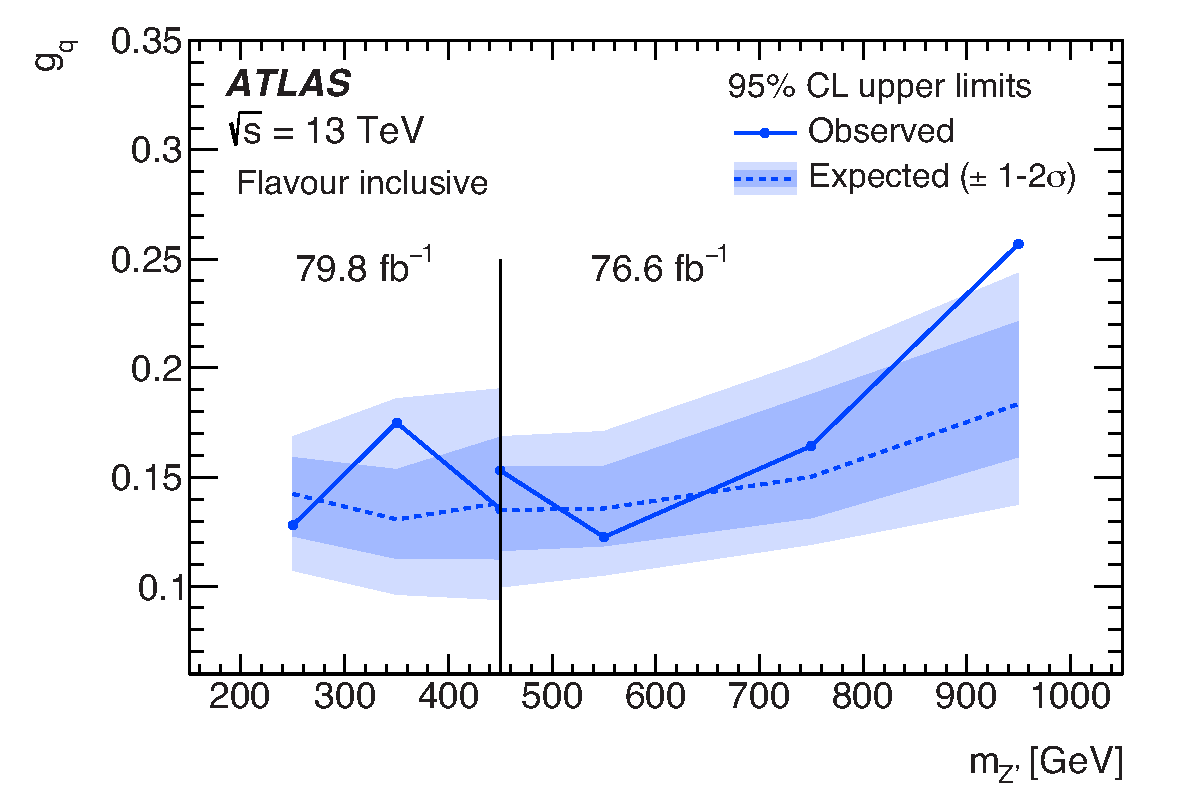
\includegraphics[width=\textwidth]{figures/ISR_resolved/2dlimits/Limits_2D_inclusive.pdf}
%	\caption{Flavour-inclusive}
	\caption{\label{fig:limit_single_inc_0p2}}
  \end{subfigure}
  \begin{subfigure}[b]{0.49\textwidth}
	  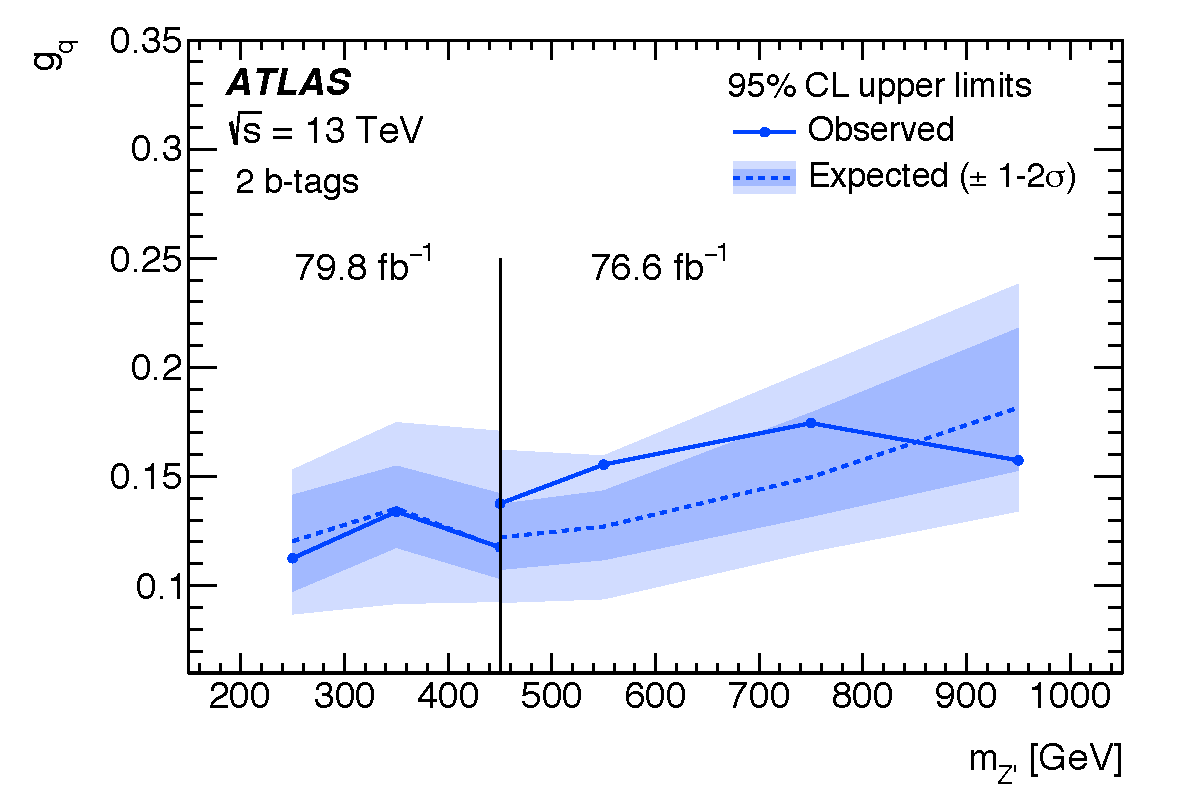
\includegraphics[width=\textwidth]{figures/ISR_resolved/2dlimits/Limits_2D_btagged.pdf}
%	\caption{\btagged}
    \caption{\label{fig:limit_single_btag_0p2}}

  \end{subfigure} \\
  \caption[Upper limits on $\Zprime$ contributions]{
    Excluded values of the coupling between a $\Zprime$ and quarks, at 95\% CL, as a function of $m_{\Zprime}$, from \subref{fig:limit_single_inc_0p2} the flavour-inclusive and \subref{fig:limit_single_btag_0p2} the \btagged categories.
    Below $450\,\GeV$ the distribution of events selected by the single-photon trigger is used for hypothesis testing, while above $450\,\GeV$ the combined trigger is used.} \label{fig:limits_zprime}
\end{figure}

\begin{figure}
  \centering
  \begin{subfigure}[b]{0.49\textwidth}
    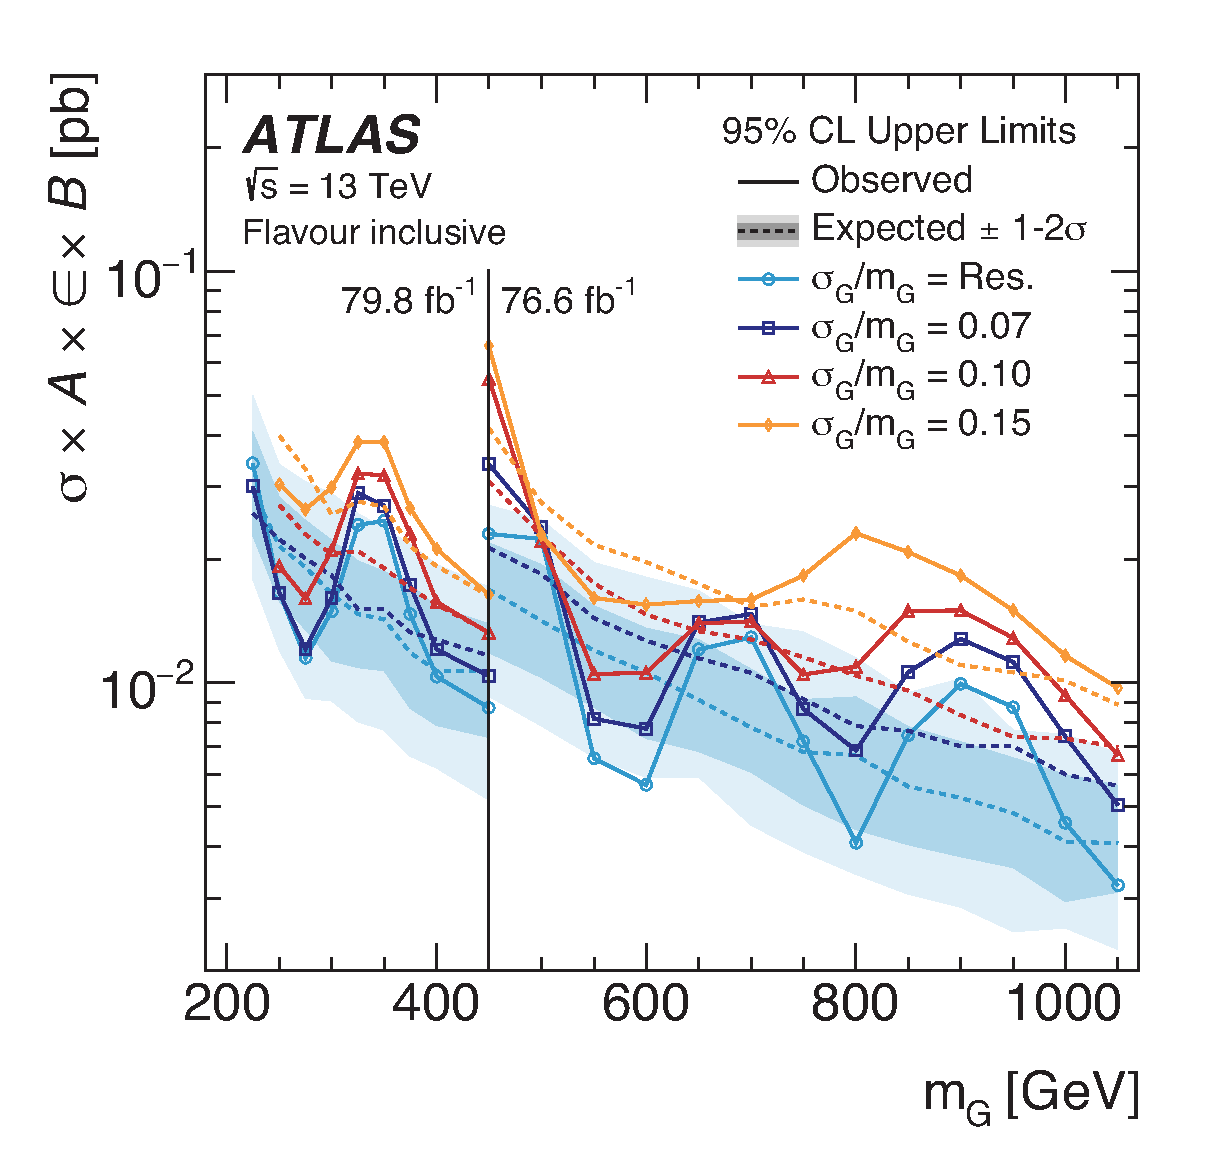
\includegraphics[width=\textwidth]{figures/ISR_resolved/GenericGaussians_CombinedInc}
	  %% \caption{Flavour-inclusive}
	  \caption{\label{fig:limit_gaussian_inc}}
  \end{subfigure}
  \begin{subfigure}[b]{0.49\textwidth}
    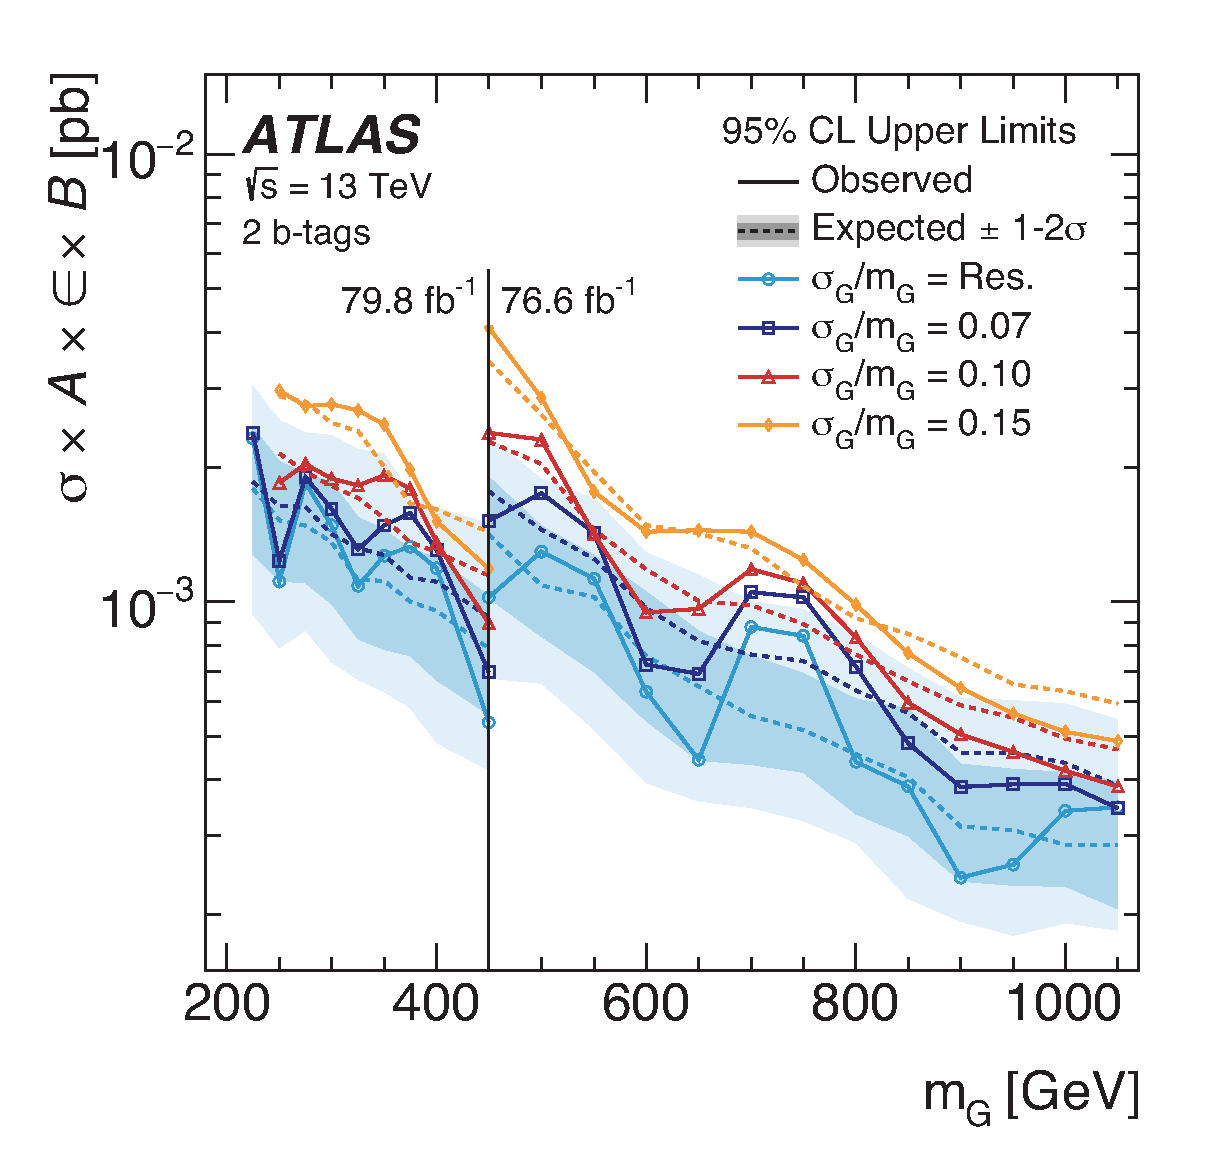
\includegraphics[width=\textwidth]{figures/ISR_resolved/GenericGaussians_Combined2b}
	  %% \caption{\btagged}
	  \caption{\label{fig:limit_gaussian_btag}}
  \end{subfigure}
  \caption[]{Upper limits on Gaussian-shape contributions to the dijet mass distributions from \subref{fig:limit_gaussian_inc} the flavour-inclusive and \subref{fig:limit_gaussian_btag} the \btagged categories.
    The curve denoted ``Res.'' represents the limit on intrinsically narrow contributions with Gaussian mass resolution ranging from 8\% to 3\% for the mass range considered.
    Below $450\,\GeV$, the distribution of events selected by the single-photon trigger is used for hypothesis testing, while above $450\,\GeV$ the combined trigger category is used.
    While the vertical axis is shared between the two selections, the signal acceptance is not the same below and above the line, and this results in different limits for the $450\,\GeV$ resonance mass point. 
    Thus the two sets of limit points correspond to two different interpretations of the product of cross-section, acceptance, efficiency, and branching ratio, $\sigma \times A \times \epsilon \times \mathcal{B}$.}
  \label{fig:limits_gaussian}
\end{figure}

%The limit setting method uses a constant prior for the signal cross-section and Gaussian priors for nuisance parameters corresponding to systematic uncertainties.
%The expected limits are calculated using pseudo-experiments generated from these priors, centred around the best fit model from the search phase.

%% The limits on the coupling $\gq$ are obtained from the cross-section limits on nearby discrete model points using the fact that the signal cross-section scales with $\gq^2$.

A more generic set of limits is shown in Fig.~\ref{fig:limits_gaussian}. These limits apply to the visible cross-section from a Gaussian-shape contribution to the $\mjj$ distribution, where the visible cross-section is defined as the product of the production cross-section, the detector acceptance, the reconstruction efficiency, and the branching ratio, $\sigma \times A \times \epsilon \times \mathcal{B}$.
The Gaussian-shape contributions have mass $m_\mathrm{G}$ and widths that span from the detector mass resolution, denoted ``Res.'' in the figure, ranging from 8\% to 3\% for the mass range considered, for an intrinsically narrow resonance, up to 15\% of the mean of the Gaussian mass distribution.

%% Limits are set only when $m_G$ is within at least twice the width of the Gaussian from the endpoints of this range.

%% This places 95\% CL upper limits on the cross-section times acceptance (visible cross-section) for new processes producing a photon or a jet and a resonance jet pair.
%% As the width increases, the expected signal contribution is distributed across more bins.
%% Therefore wider signals are affected less than narrower signals by statistical fluctuations of the data in a single bin. The searches have reduced sensitivity to wider signals compared to narrower signals.

%% For sufficiently narrow resonances, the results obtained for Gaussian signals may be used to set limits in BSM models beyond the one considered explicitly in this note. 
%% These limits can be used when off-peak contributions to the reconstructed $\mjj$ distribution predicted by the BSM model, such as those due to jet-combinatorics, PDF, and non-perturbative effects~\cite{Harris:2011bh}, can be safely neglected or truncated, leaving a Gaussian core. This is the case of the  $\Zprime$ axial vector signals used as benchmark in these searches. Signals with an intrinsic width much smaller than 5\% should be compared to the limit curve for a width equal to the experimental resolution.
%% Predicted signals with larger widths should be compared with the limit that corresponds most closely to the width of the Gaussian contribution predicted by the model.
%% More instructions can be found in Appendix A of Ref.~\cite{EXOT-2013-11}.

Both the choice of fit function and statistical fluctuations in the $\mjj$ distribution can contribute to uncertainties in the background model.
To account for the fit function choice, the largest difference between fits among the variants of Eq.~(\ref{eq:ua2}) and~ Eq.~(\ref{eq:5par}) that obtain a $p$-value above 0.05, is taken as a systematic uncertainty.
The uncertainty related to statistical fluctuations in the background model is computed via Poisson fluctuations around the values of the nominal background model.
The uncertainty of the prediction in each $\mjj$ bin is taken to be the standard deviation of the predictions from all random samples.

The reconstructed signal mass distributions are affected by additional uncertainties related to the simulation of detector effects.
The jet energy scale uncertainty is applied to the $\Zprime$ mass distributions using a four-principal-component method~\cite{PERF-2016-04,ATL-PHYS-PUB-2015-014,ATL-PHYS-PUB-2015-015}, leading to an average 2\% shift of the peak value for each mass distribution.
For the Gaussian-shape signal models, this average 2\% shift is taken as the uncertainty of the mean of each Gaussian distribution.
In the case of the \btagged\ categories, uncertainties of the \btagging\ efficiency are the dominant uncertainties in each mass distribution.
To account for these uncertainties, the contribution of each simulated event to a given mass distribution is reweighted by 5\%--15\% for each jet, depending on its $\pt$~\cite{PERF-2016-05}.

The remaining uncertainties are modelled by scaling each simulated distribution by 3\% to account for jet energy resolution in all categories~\cite{PERF-2016-04}, 2\% for photon identification uncertainties in the single-photon-trigger categories and 1.4\% in the combined-trigger categories~\cite{PERF-2017-02}, 3\% to account for efficiencies of the combined trigger, and 1\% for PDF-related uncertainties (only applied to the mass distributions of $\Zprime$ signals).

All these uncertainties are included in the reported limits; further uncertainties of the theoretical cross-section for the \Zprime model are not considered.

The uncertainty of the combined 2015--2017 integrated luminosity is derived following a methodology similar to that detailed in Ref.~\cite{DAPR-2013-01} and using the LUCID-2 detector for the baseline luminosity measurements in 2017~\cite{LUCID2}.
The estimates for the individual datasets are combined and applied as a single scaling parameter with a value of 2\% for the single-photon-trigger categories and 2.3\% for the combined-trigger categories.

%-------------------------------------------------------------------------------
\section{Conclusion}
%% \label{sec:conclusion}
%-------------------------------------------------------------------------------

Dijet resonances with a width up to 15\% of the mass, produced in association with a photon, were searched for in up to $79.8\,\ifb$ of LHC $pp$ collisions recorded by the ATLAS experiment at $\sqrt{s}=13\,\TeV$. The observed $\mjj$ distribution in the mass range $169\,\GeV < \mjj < 1100\,\GeV$ can be described by a fit with smooth functions without contributions from such resonances.

%no significant evidence of resonant phenomena beyond the Standard Model is seen in the mass range $225\,\GeV < \mjj < 1100\,\GeV$.

In the absence of a statistically significant excess, limits are set on two models: $\Zprime$ axial-vector dark-matter mediators and Gaussian-shape signal contributions.
All mediator masses within the analysis range are excluded for a coupling value of $\gq = 0.25$ and above, with the exclusion limit near a coupling of $\gq=0.15$ for most of the mass range.
The \btagged categories yield $\Zprime$ limits comparable to the flavour-inclusive categories, assuming that the $\Zprime$ decays equally into all quark flavours, and provide model-independent limits that can be reinterpreted in terms of resonances decaying preferentially into $b$-quarks.
For narrow Gaussian-shape structures with a width-to-mass ratio of 7\%, the flavour-inclusive categories exclude visible cross-sections above 12~fb for a mass of 400~\GeV and above 5.1~fb for a mass of 1050~\GeV.
When wider signals with a width-to-mass ratio of 15\% are considered, the exclusion limits are weaker at the lower mass values, with visible cross-sections above 21~fb excluded for a mass of $400\,\GeV$ and those above 9.7~fb excluded for a mass of $1050\,\GeV$. 

These results significantly extend the constraints by ATLAS and other experiments at lower centre-of-mass energies on hadronically decaying resonances with masses as low as 225 GeV and up to 1100 GeV.


%\include{sections/chapter_SearchForBoostedDijetISR}
%\chapter{The Resonance Search on the Dimuon Signature}
\label{chapter:dimuon}

\section{Introduction}

    % Why this is interesting  
    Owing to its unprecedented high energy, the run I and early run II of ATLAS has long focused on the high mass resonances searches. This has left some gaps in the low mass region that are unexplored. In the two lepton final state, there has been an analysis after the Z boson peak since the beginning of Run 1, however the mass region below the Z mass peak has left a region totally uncovered on ATLAS.

\begin{figure}[!htb]
    \begin{center}
        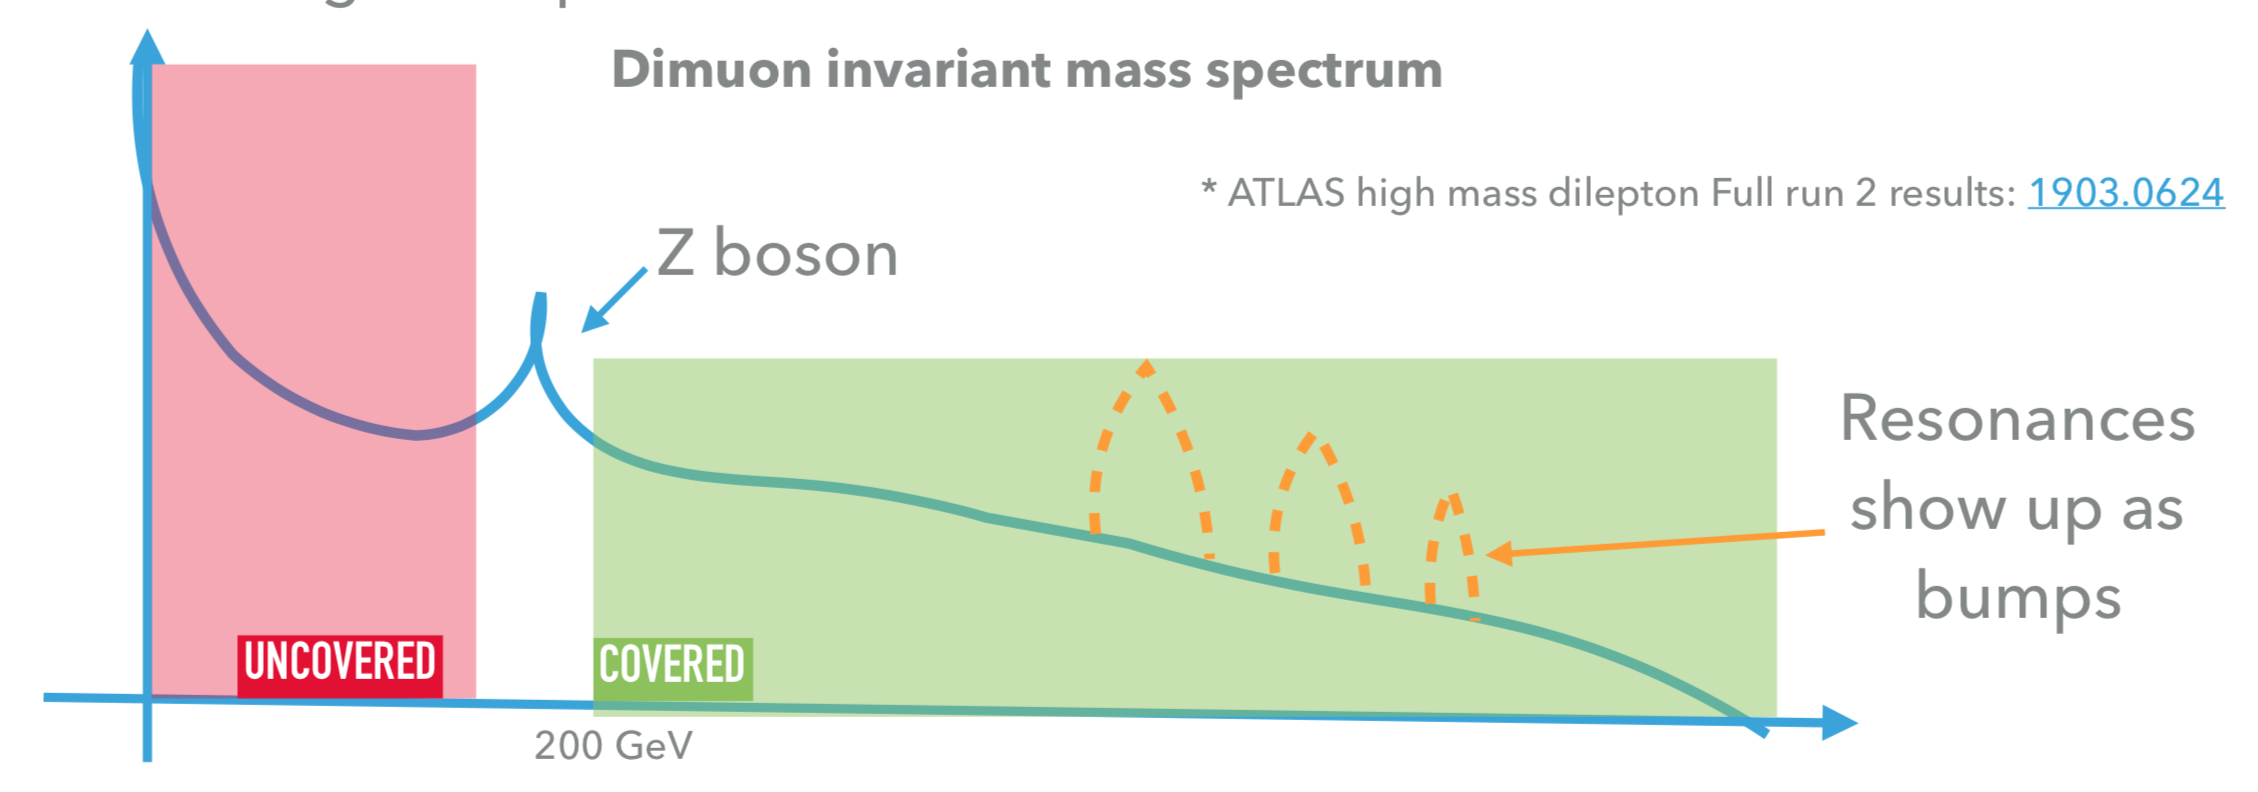
\includegraphics[width=0.75\textwidth]{figures/chapter_dimuon/dimuonStudies}        
        \caption{
        This cartoon illstrate the target signal region of the analysis and how it has not been covered by the previous high-mass dilepton analysis. }
            \label{fig:dimuonstudies}
    \end{center}
\end{figure}
   
    Since ATLAS collide partons, there are fewer background on leptons than jet processes, this allows lower transverse momentum lepton events to be saved. Using two muons as the resonance final state items, lower mass resonances can be searched for, going below the limits of the dijet resonances. The signal significance would be higher compared to jet. 

    This search results is interesting to the theoretical community for the dark matter benchmark interpretation possible.

%\section{Historical searches}    
%    Previous searches has been done directly in Tevatron experiment. Indirect constraints has been made in LEP as well. 
%
%    CMS results and tevatron results: 
%    
%    This study will be an independent finding from ATLAS and the first search done in this region.  


\section{The Search Channels}
Since there is a trigger turn-on feature near 45 GeV in the distribution due to the cut in muon transverse momentum in trigger, 
This analysis is based on a pheno-study first done here\cite{2014}.

There are two search channels in the analysis, each covering a different mass region, namely the boosted and the 

\begin{figure}[!htb]
    \begin{center}
        \includegraphics[width=0.75\textwidth]{figures/chapter_dimuon/turnedon}
        \caption{
        this figure shows the trigger turn on curve in the inclusive dimuon channel, and how utilizing the boosted channel a smooth background is possible in the lower mass region from 10-45 gev. samples used here are from the monte carlo sample in section~\ref{}, a minimal cut of muon pt >14 gev are done on the two leading muons. }
            \label{fig:turnon}
    \end{center}
\end{figure}

\section{Signal Theoretical Model}

    The analysis uses the dark matter LHC benchmark model and dark photon model outlined in~\ref{sec:LHCDM}.
Other models that are of interest and can be searched for in this analysis includes the W', the quantum blackholes,and axion models. 
The following search focuses on the search on the vector dilepton signature from the dark photon model and the dark matter benchmark. But as Gaussian limits are also set, the results will be reinterpretable for many other models that predicts scalar or axion-vector resonances. 

\begin{figure}[!htb]
    \begin{center}
        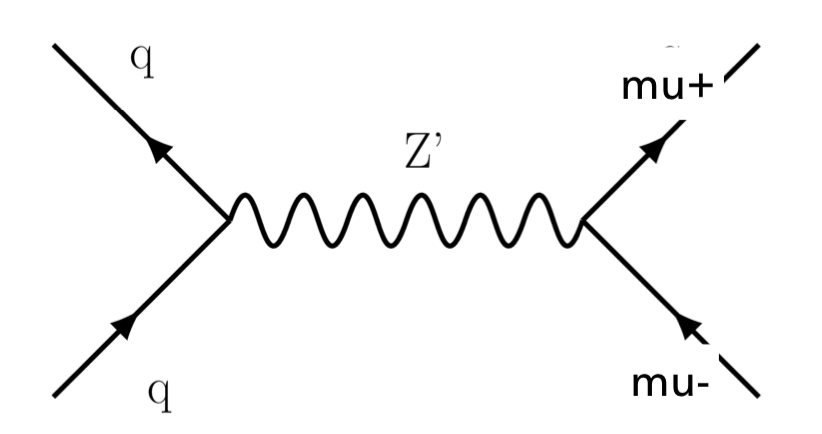
\includegraphics[width=0.75\textwidth]{figures/chapter_dimuon/dimuonFeynman}
        \caption{
            This figure shows the Feynmann diagram of the inclusive dimuon signal as the signal for the analysis. }
            \label{fig:dimuonFeynmann}
    \end{center}
\end{figure}


\begin{figure}[!htb]
    \begin{center}
        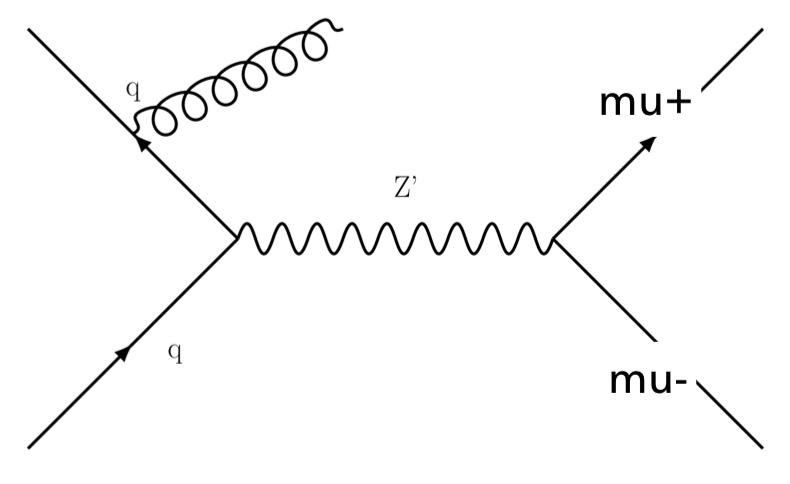
\includegraphics[width=0.75\textwidth]{figures/chapter_dimuon/dimuonISRFeynmann}
        \caption{
        This figure shows the Feynmann diagram of the boosted dimuon ISR signa used as the signal for the analysis. }
            \label{fig:dimuonFeynmann}
    \end{center}
\end{figure}

    The different signal distributions across different kinematics are shown here. 

\begin{figure}[!htb]
    \begin{center}
        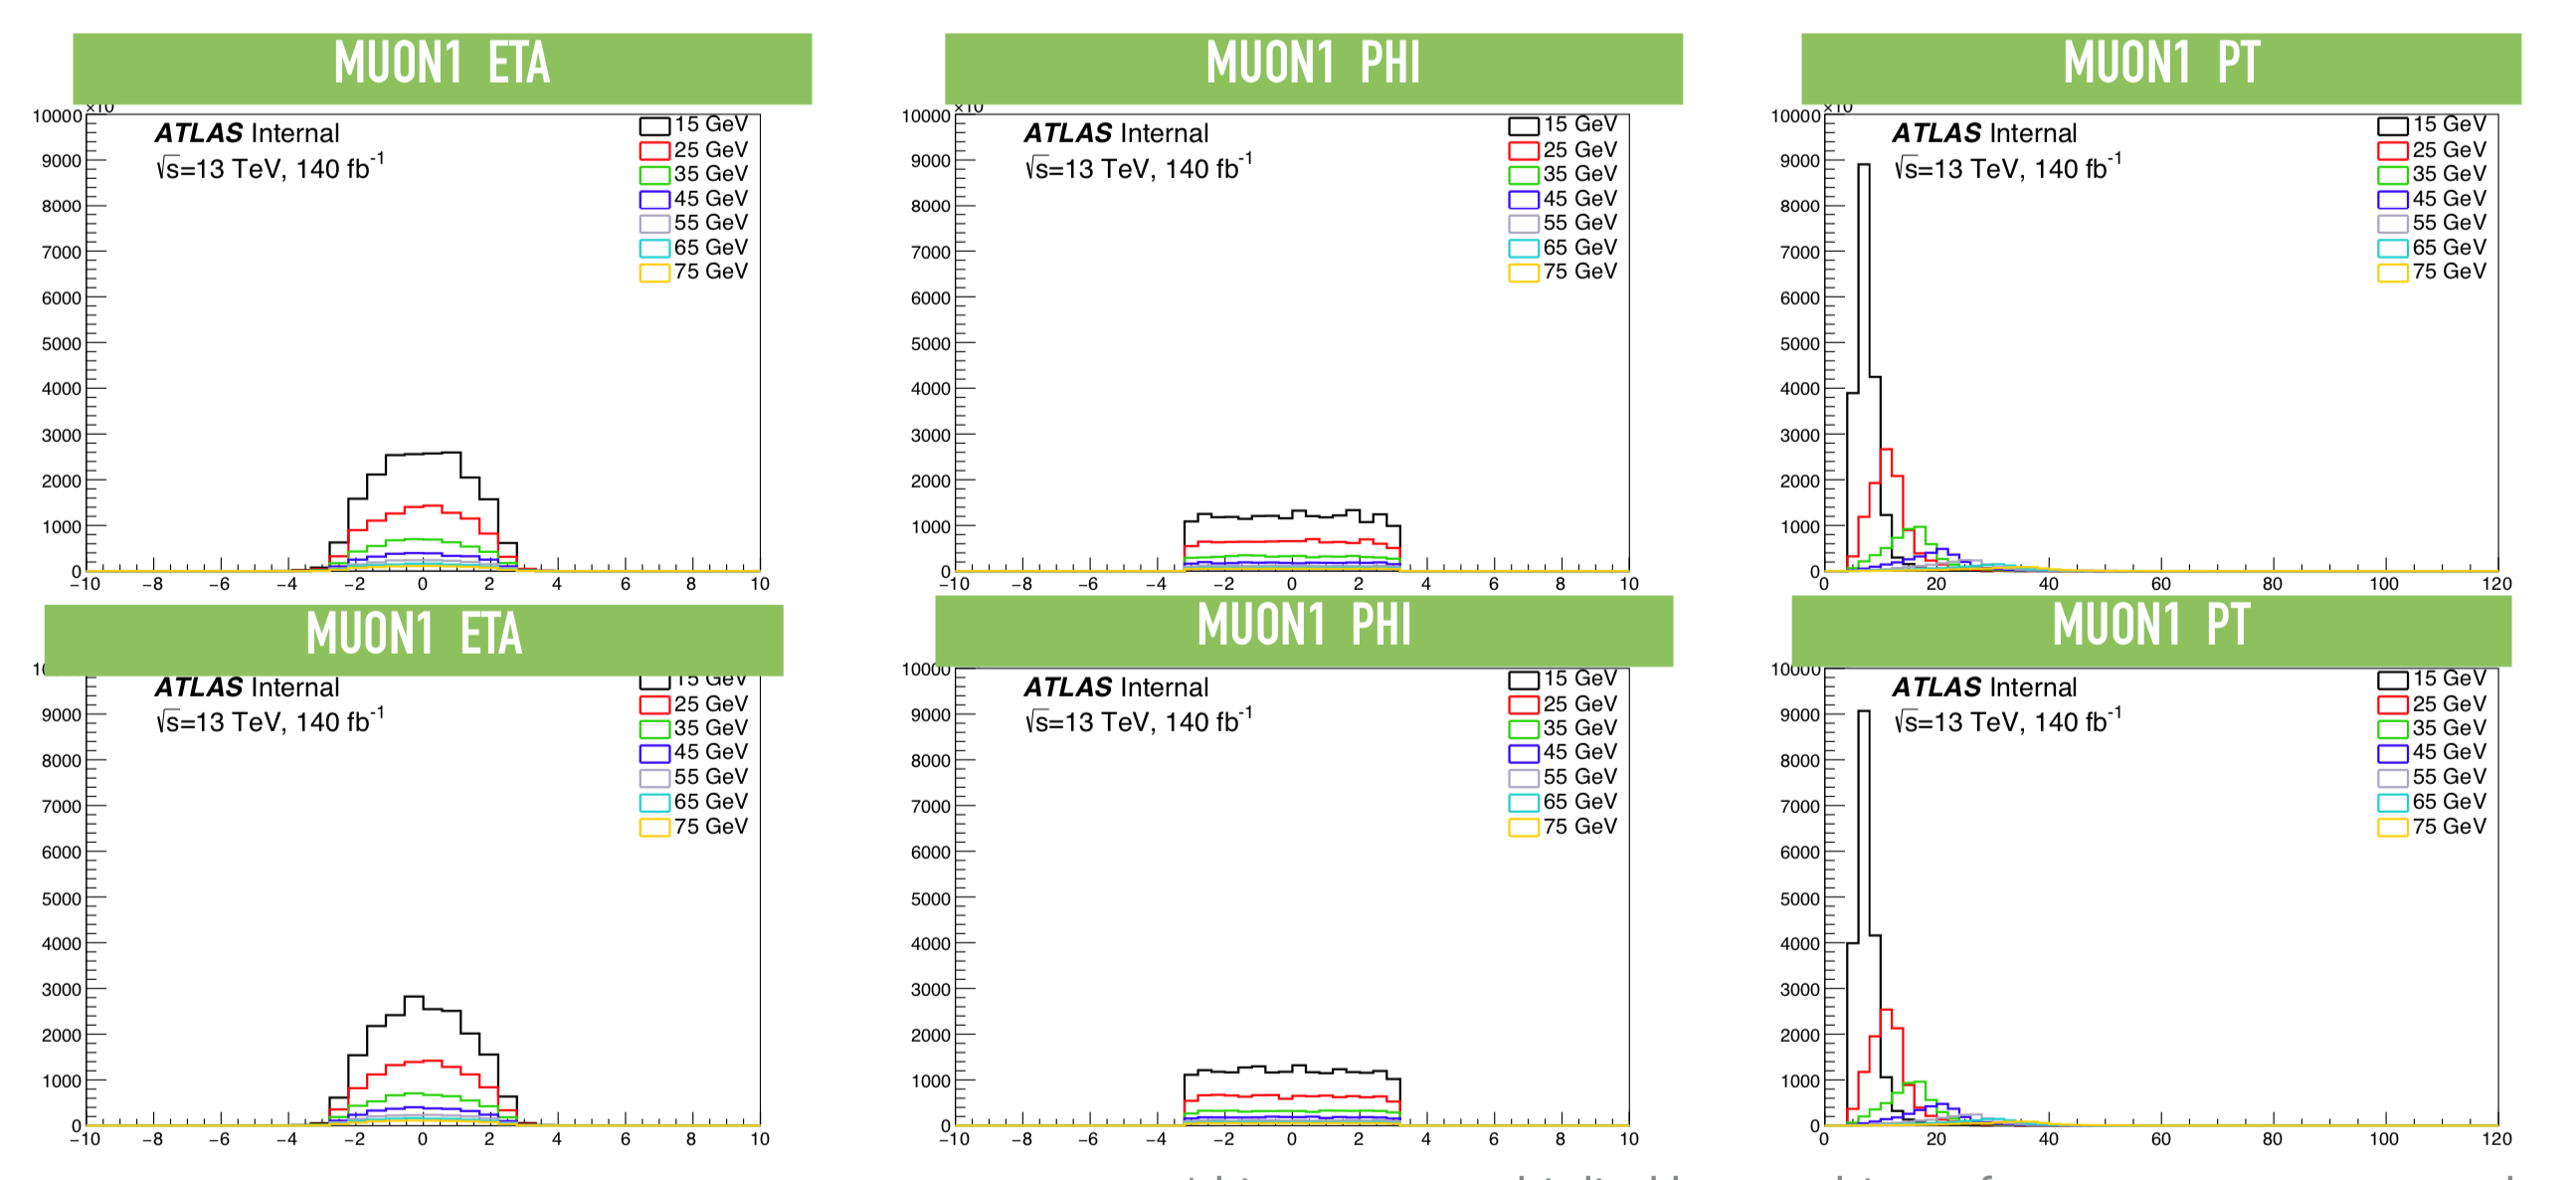
\includegraphics[width=0.75\textwidth]{figures/chapter_dimuon/dimuondist1}
        \includegraphics[width=0.75\textwidth]{figures/chapter_dimuon/dimuondist2}
        \includegraphics[width=0.5\textwidth]{figures/chapter_dimuon/dimuondist3}
        \includegraphics[width=0.2\textwidth]{figures/chapter_dimuon/dimuondist4}
        \caption{
        This figure shows the signal distribution of the inclusive dimuon samples generated. A minimal cut of muon pt >14 gev are done on the two leading muons. }
        \label{fig:dimuon}
    \end{center}
\end{figure}


\begin{figure}[!htb]
    \begin{center}
        \includegraphics[width=0.75\textwidth]{figures/chapter_dimuon/dimuonISRdist1}
        \includegraphics[width=0.5\textwidth]{figures/chapter_dimuon/dimuonISRdist2}
        \includegraphics[width=0.5\textwidth]{figures/chapter_dimuon/dimuonISRdist3}
        \includegraphics[width=0.2\textwidth]{figures/chapter_dimuon/dimuonISRdist4}
        \caption{
        This figure shows the signal distribution of the boosted dimuon samples generated. A minimal cut of muon pt >14 gev are done on the two leading muons. }
       \label{fig:boosted}
    \end{center}
\end{figure}


\section{Data preparation}

\subsection{Samples Used for the Analysis}
The following are the samples used for the analysis.

\begin{table}[!htb]
    \begin{center}
    \caption{
        The table shows the Monte Carlo dataset used for the analysis. 
    }
\label{tab:MC samples}
\begin{tabular}{|l|l|}
\hline
\textbf{MC Type}   & \textbf{DSID}                                                         \\ \hline
Z+ jets $\mu\mu$   & 364100 - 364113 , 364198-364203                                       \\ \hline
Z+jets $\tau \tau$ & 364128 - 364141 , 364210-364215                                       \\ \hline
$t\bar{t}$         & 410472                                                                \\ \hline
Diboson Sherpa     & 364253 - 364255 , 363355 - 363360 ; 363489 ; 364250 ; 364288 - 364290 \\ \hline
Top decay          & 410644 - 410645 , 410658 - 410659 ; 410648 - 410649                   \\ \hline
W + jets munu      & 364156 - 364169                                                       \\ \hline
$b\bar{b}$         & 363833                                                                \\ \hline
$c\bar{c}$         & 363834                                                                \\ \hline
\end{tabular}
\end{center}
\end{table}


\begin{table}[!htb]
    \begin{center}
    \caption{
        The table shows the Data dataset used for the analysis. 
    }
\label{tab:MC samples}
\begin{tabular}{|l|l|}
\hline
\textbf{Data Taking year}   & \textbf{Data Period} \\ \hline
2015   & D-J                                       \\ \hline
2016   & A-L                                       \\ \hline
2017   & B-F, H                                    \\ \hline
2018   & B-F, I, K, L-O, Q                         \\ \hline
\end{tabular}
\end{center}
\end{table}


\subsection{Trigger Chain}
The analysis takes the "OR" of the three trigger chains :

\begin{itemize}
    \item{HLT_2mu14}
    \item{HLT_mu22_mu8noL1}
    \item{HLT_mu26_ivarmedium}
\end{itemize}

\begin{figure}[!htb]
    \begin{center}
        \includegraphics[width=0.75\textwidth]{figures/chapter_dimuon/TriggerChain}        
        \caption{
        This cartoon illstrate the trigger used for the different trigger region. A is HLT_2mu14, B represents HLT_mu22_mu8noL1; C shows HLT_mu26_ivarmedium. }
    \end{center}
\end{figure}

%The efficiency are calculated for each region for the subsequent weighting of in the trigger scale factor.
%\begin{equation}
%    SF= \epsilon_{data}/\episilon_{MC}
%\end{equation}

\subsection{Background composition}
The background composition of the Monte Carlo is shown here:

\begin{figure}[!htb]
    \begin{center}
        \includegraphics[width=0.75\textwidth]{figures/chapter_dimuon/backgroundcomposition}
        \includegraphics[width=0.75\textwidth]{figures/chapter_dimuon/backgroundcomposition2}
        \caption{
        This cartoon illstrate the background composition of the samples }
    \end{center}
\end{figure}

\subsection{Event Selection}
Following the above trigger cuts, the following event selections are made on the muons:

\subsubsection*{Muon Working Point}
The medium working point is chosen for the muons, details to the working point can be found here: 

The choice is made on the medium working point over low PT, as the trigger threshold effectively cut out most muons below 8GeV. The Low PT working point only has a higher efficiency over the medium working point below  6 GeV. 

\subsubsection*{Isolation Working Point}
FixedCutPflowLoose is chosen to be the isolation working point, details on the working point description can be found here:~\ref{}. 


\subsubsection{Fake Estimation}
Fakes are objects that are not opposite signed dimuon pairs that falls into the selection requirement in data event selection due to misidentifications.
Since the fakes mainly comes from QCD ATLAS processes, the amount from same signed process and opposite signed process are approximately the same. 
Fakes in the background sample can be estimated from the same signed leptons in data. Studies found that the content is less than 1\% of all the background contribution. The estimated same signed leptons contribution is added to the MC background composition.

\begin{figure}[!htb]
    \begin{center}
        \includegraphics[width=0.75\textwidth]{figures/chapter_dimuon/backgroundcomposition}
        \caption{
        This cartoon illstrating the amount of fakes in the background composition. SS refers to same signed lepton in the data sample set, whereas OS refers to the opposite sign lepton pairs in data. }
    \end{center}
\end{figure}

\subsubsection{Superfast dimuon samples}
Due to the low statistics in the primary background sample in  Z > \mu \mu, fast generation relying on Pythia8 and a smearing function for the detector effect has been used to lower the statistical fluctuation. More details on the fast simulation can be found in the Higgs to $\mu \mu $ int note.

%\subsection{Sensitivity Test}
%Sensitivity test is done on the 

\subsection{Dimuon Mass Spectrum Resolution}
The mass spectrum resolution are done on the Powheg samples of Z > $\mu \mu
$. A Gaussian distribution fit is performed on the resonance mass $m_{\mu\muTruth} - m_{\mu\muReco}$ quantity. From the fit, the width of the Gaussian is obtained~\ref{fig:fit}, and is shown to follow the following distribution in figure~\ref{fig:sigma}.

\begin{figure}[!htb]
    \begin{center}
        \includegraphics[width=0.75\textwidth]{figures/chapter_dimuon/fitError}        
        \caption{
            A Gaussian distribution fit is made on the the difference between the truth dimuon resonance mass and the reconstructed dimuon resonance mass. }
    \end{center}
\end{figure}
   
\begin{figure}[!htb]
    \begin{center}
        \includegraphics[width=0.75\textwidth]{figures/chapter_dimuon/sigma}        
        \caption{
        From the fitted Gaussian distribution, the width is obtained for different resonance mass. They are plotted here. The width-to-mass resolution $\sigma_{m_{\mu\mu}}/m_{\mu\mu}$ is found to be close to 1.5\%.}
    \end{center}
\end{figure}


\subsection{Binning Strategy}
Using the resolution of the study from the last section and the mass distribution given in the theoretical signal section, the overall binning is chosen to be 0.25 GeV, it will allow for all signal searched for to be at least 2 bin wide. Signal that are at least two bin wide are significantly less prone to accidental "discoveries" due to statistical fluctuation.

\subsubsection{MC/Data Comparison}
A detailed description on the MC/Data comparison test can be found here,\ref{sec:MCData}.  
The agreement is shown to be good between the prepared MC and data. It shows that the MC is ready to be used for the subsequent tests.

\begin{figure}[!htb]
    \begin{center}
        \includegraphics[width=0.75\textwidth]{figures/chapter_dimuon/MCDataCompare}
        %\includegraphics[width=0.75\textwidth]{figures/chapter_dimuon/MCDataCompare2}
        %\includegraphics[width=0.75\textwidth]{figures/chapter_dimuon/MCDataCompare3}
        %\includegraphics[width=0.75\textwidth]{figures/chapter_dimuon/MCDataCompare4}
        %\includegraphics[width=0.75\textwidth]{figures/chapter_dimuon/MCDataCompare5}
        \caption{
        Monte Carlo and data comparison. A reasonable agreement is seen. Showing that the MC is ready to be used for the subsequent studies.
        }
    \end{center}
\end{figure}

\section{Background Fitting}

The Gaussian process background fitting method is being used for this study, a back-up fit function method is also used. Details on how these methods are motivated can be found here~\ref{section:backgroundest}.  

\subsection{Gaussian Process}

The Gaussian process background and signal kernels are given as cited here~\ref{sec:kernel}.

The minimum background lengthscale is studied through the signal injection test described here~\ref{signalInjection}.

Signal of mass widths of 1\%, 3\% and 5\% of different sizes are injected into the mass spectrum. It's found that a minimum lengthscale of 4 GeV is needed for the background kernel for the background model to be sensitive to signal of 3\sigma background error size and above.


\subsubsection{Signal injection test}
\begin{figure}[!htb]
    \begin{center}
        \includegraphics[width=0.75\textwidth]{figures/chapter_dimuon/signalInjection}        
        \caption{
        This figure illustrate a signal injection test performed at the mass point  }
            \label{fig:dimuonstudies}
    \end{center}
\end{figure}

\subsubsection{Background Modelling}
Using the minimal lengthscale chosen for the background and allowing other hyperparameters to float, tests fits are performed on the nominal fit, and also done on the different statistical variation of the background, the 1 $\sigma$ up and 1 $\sigma$ down variation of the fast simulation Pythia, as well as the $\eta$ variation.
The fitting result shows that Gaussian Process works well for all of these statistical variations. 

\begin{figure}[!htb]
    \begin{center}
        \includegraphics[width=0.75\textwidth]{figures/chapter_dimuon/Nominal}        
        \includegraphics[width=0.75\textwidth]{figures/chapter_dimuon/NominalBH}        
        \includegraphics[width=0.75\textwidth]{figures/chapter_dimuon/NominalFit}        
        \caption{
        These figure illustrates the nominal fit, along with the bumphunter test statistics and the observed value distribution. It's shown that the most discrepant window does not fall below the critical p-value of 0.01. Details on the bumphunting procedure can be found here. }
            \label{fig:dimuonstudies}
    \end{center}
\end{figure}


\begin{figure}[!htb]
    \begin{center}
        \includegraphics[width=0.75\textwidth]{figures/chapter_dimuon/UpVariation}
        \includegraphics[width=0.75\textwidth]{figures/chapter_dimuon/DownVariation}
        \includegraphics[width=0.75\textwidth]{figures/chapter_dimuon/EtaVariation}
        \caption{
        These figure illustrates the Gaussian Process background fits on the different variation of the MC generated. }
    \end{center}
\end{figure}



\subsection{Spurious signal test}
Details on the spurious signal can be found here~\ref{spurious}.
The spurious signal test results on the Gaussian process is shown here:

\begin{figure}[!htb]
    \begin{center}
        \includegraphics[width=0.75\textwidth]{figures/chapter_dimuon/spurious}        
        \caption{
        This figure illustrate a spurious signal test result on the different background variation fits.}
            \label{fig:dimuonstudies}
    \end{center}
\end{figure}


\section{Statistics Testing}
Details on the statistical test can be found here~\ref{}. During the time where the thesis was written, the data was not unblinded. Monte Carlo studies were done. A sample signal is injected into the spectrum to test the bumphunter, and the limit is generated using background MC assuming no signal was found.

\section{The Search}
A sample signal the size of 3$\sigma$ background error is injected into the spectrum, the test is done to illustrate that the search is capable of picking out the signal.
    


\begin{figure}[!htb]
    \begin{center}
        \includegraphics[width=0.75\textwidth]{figures/chapter_dimuon/signalinjected}
        \includegraphics[width=0.75\textwidth]{figures/chapter_dimuon/signalinjected2}
        \caption{
        These figures illustrate a test done on signal injected at 55 GeV, and the window exclusion that picked out the signal injected in there.}
%            \label{fig:dimuonstudies}
    \end{center}
\end{figure}

section{Limit Setting}
Preliminary limit setting is still currently under test, figure\ref{} shows a preliminary result from the Asimov method. 

begin{figure}[!htb]
   \begin{center}
       \includegraphics[width=0.75\textwidth]{figures/chapter_dimuon/limits}       
       \caption{
       This figure illustrate a spurious signal test result on the different background variation fits.}
            \label{fig:dimuonstudies}
   \end{center}
end{figure}

n alternative fit function limits calculated by approximation based on the fit function method is shown here, it's expected that the analysis will have comparible sensitivity to LHCb. 

begin{figure}[!htb]
   \begin{center}
       \includegraphics[width=0.75\textwidth]{figures/chapter_dimuon/limits}
       \caption{
       This figure illustrate a spurious signal test result on the different background variation fits.}
            \label{fig:dimuonstudies}
   \end{center}
end{figure}



section{Future Work}
he analysis is on its way to completing the final strategies and to be unblinded on data soon.

\section{Alternative fitting}
An alternative fitting method is done through the fit function method.

\section{Systematics}
section{Future Extensions}


%
\chapter{Future Resonance Finding}
\label{chapter:weird}

0. Introduction

1. Trigger level analysis

2. Future of resonance finding

3. Statisitcal method  


%\chapter{Concluding Words: Anomalous Resonance as a Question}

%So tell me, what is it that I do not know?
%Anomalous resonances as a question to what can be looked for in physics
%A question in disguise
% add projected exclusion plot 

%I had a dream where I swallowed a cheerio shaped hole. 
%In a dream I swallowed a cheerio shaped hole.
%The question in the form of a bump.%
%This is not a search but rather a question in disguise. 
% Search claims thhat we actually do know someonthing about the bump.
% queer in search of joussance 

%\epigraph{\textit{The bud disappears when the blossom breaks through, and we might say that the former is refuted by the latter; in the same way when the fruit comes, the blossom may be explained to be a false form of the plant’s existence, for the fruit appears as its true nature in place of the blossom. The ceaseless activity of their own inherent nature makes these stages moments of an organic unity, where they not merely do not contradict one another, but where one is as necessary as the other; and constitutes thereby the life of the whole.}}{--Georg Hegel}

Particle physics has come a long way since its early days. Since the discovery of the Higgs Boson in 2012, the Standard Model is considered completed. But human's quest to understand fundamental physics is far from over. Many existing issues in Standard Model points to a picture out there unknown, yet to be understood. This evidence, especially those concerning Dark Matter, drove the resonance search analyses presented in Chapter~\ref{chapter:dijetISR} and Chapter~\ref{chapter:dimuon}.
However, as a highly distinguishable signature, resonances hunting offers much more than a tool to hunt for a specific candidate. In the age where most exotic and SUSY searches returned empty results, what ought to concern physicists regarding data is no longer merely what can be searched for, but also what can be \textit{asked}: what questions can be asked of data for them to reveal to us what we do not know? This chapter summarizes some directions that can be taken in the resonance hunting regime for future studies.
%But the search for the little bump is perhaps not just a search
%for dark matter, it is also a question on what is possible to be searched for and what lies between the boundaries of the known and unknown of our understanding. What is it that we do not know about? 


%Perhaps the gauge of what a physicist
%
%But human's search for truth is far from that.  However, along with all the compelling evidence, a complete physics theory is out there to be discovered. The analyses presented in Chapter~\ref{chapter:dijet} and Chapter~\ref{chapter:dimuon} both offered results important to answering of the question of Dark Matter. But in the age where new physics
%theory seems to be out of reach with most evidence, the quest of resonance hunting, is perhaps not merely to search for a theoretical candidate to what's out there. Is not in actuality a search, but rather, is a question in disguise. 
%What is possible for us to look for? The little bumps like signature is what lies between the known and the unknown of our understanding? Future lies in good miner and searcher for new things, it lies in physicists being good question askers in coaxing data from telling us its stories. 
%As a highly distinguishable signature, resonances not just a tool for catch, but also a question we can ask on what borders between the known and unknown. 
%
%the more compelling question that these analyses is no longer a particular theory candidate, but instead, to ask what is possible to be looked for?
%
%Instead the search for resonances, in their various methods, can be thought of as asking 
%
%the search for a more complete understanding to the nature of the world is far from over. One way to further our search is through these ripple nuggets of resonances. Driven by the question of Dark Matter, the analyses presented in Chapter~\ref{chapter:dijet} and Chapter~\ref{chapter:dimuon} bothoffers additional evidence to the search of the
%Dark Matter mediator Z'. The searches are also important in the following way, namely they extends beyond the previous ground and explored new tools for future resonance hunting effort. perhaps it's offering an alternative not just in the search but also in the method itself. Instead of 
%what is it possible to be looked for? 


%Figure here shows the dark matter exclusion limit plots from the dark matter chapter.

\section{Unexplored Landscape of the Two Body Resonances}
Chapter~\ref{chapter:topo} explored uncovered two-body final states in resonance hunting in detail. The paper has since been superseded by newer results ~\cite{2020}. The surveys offer an overview of all two-body final states that are left unsearched for in collider physics that could provide a wealth of sources for possible places to look for new physics signatures.

\section{Gaussian Process as a Background Modeling Method}
The Gaussian Process-based background estimation method is currently being finalized in ATLAS with the dimuon analysis in Chapter~\ref{chapter:dimuon}. It provides a more flexible method better suited for high luminosity for smooth background modeling for other resonance hunting analyses where MC is limited. The method offers the advantage of being \textit{generalizable} for any final state with a smooth background estimation in the signal region. The method will be applicable to many other future analyses. 
%Gaussian Process can also be extended to perform searched in the 2-dimensional search space for increased signal sensitivity.

\section{Data Scouting}
Due to limited bandwidth, the trigger described in Chapter~\ref{chapter:dimuon} set a lower bound in the mass of the resonance that could be searched for. Searching for a signal with initial state radiation mitigates this but it also results in a lowered sensitivity to the signal. Data scouting is a method proposed to create a special triggering stream and object to mitigate the limit triggering bandwidth by storing only partial events. Only information directly related to the analysis will be
stored. Currently, the dimuon data scouting analysis is under study in ATLAS and will be a future area with promising improved sensitivity. 

\section{Anomaly Detection for Resonances with Machine Learning Method}
The concept of “model-independent” searches is not unfamiliar to LHC. Searches for new particles often include model-independent results in the form of excesses beyond certain statistical significance LHC also has its dedicated general search ~\cite{General2019}. However, these current approaches are not truly model-independent: they are either signal model-dependent in the sensitivity optimal kinematic cut for targeted search or LHC background dependent in the general search. Search
sensitivity is greatly diminished if the anomaly is not as predicted by the signal or background models. An improved method will instead teach data to perform optimal selection on its own based only on the anomaly observed in data. One recent proposal is the weakly supervised Classification Without Labels (CWoLa) hunting method~\cite{CWoLA2019}. This technique discards the usual supervised Signal-over-background (S/B) kinematic strategy, where the optimal selection is made based on
the maximal S/B ratio of a specific model combination. In utilizing CWoLa for resonance hunting, the bump-like signal produces a signal-rich center-band and signal-deprived side-bands optimal for optimal sensitivity kinematic cuts training. If a new particle is embedded in the dataset, CWoLa training will produce a selection cut that maximizes events in the central-band-bump without any underlying S/B model assumptions. The data is made to reveal surprising anomalies on its own from the data alone.
The existing two-quark final state resonance CWoLa search~\cite{CWOLA2020} to other final states including muons, photons, and other uncovered resonance signatures. While the dijet analysis has proven the feasibility of the method in ATLAS, many detailed technical aspects, further generalizations, and expansions into larger feature spaces must still be performed. The new analyses on muon and photon final states will go beyond the predecessor by focusing the training on additional features including
the jet substructure of the ISR jet. More complicated signal topologies, where the primary resonant decay object can be composite, can also be explored using simpler muon/photon final state objects. The CWoLa model-independent searches will serve as complementary additions to current physics analyses’ model-dependent and independent search methods, and it will push sensitivity into new regions with attuned understanding driven by the data itself. 

%otheer anomaly searches are driven by-%rthe. It could open a new chapter where data are made to tell the truth behind. 


%\include{sections/chapter1}
%\include{sections/chapter2}
%\include{sections/chapter3}
%\include{sections/chapter4}
%\include{sections/chapter5}
%\include{sections/chapter6}
%\include{sections/chapter7}
%\include{sections/chapter8}
%\include{sections/chapter9}
%\include{sections/chapter10}

% These commands fix an odd problem in which the bibliography line
% of the Table of Contents shows the wrong page number.
\clearpage
\phantomsection

% "References should be formatted in style most common in discipline",
% abbrv is only a suggestion.



% The Thesis Manual says not to include appendix figures and tables in
% the List of Figures and Tables, respectively, so these commands from
% the caption package turn it off from this point onwards. If needed,
% it can be re-enabled later (using list=yes argument).
\captionsetup[figure]{list=no}
\captionsetup[table]{list=no}


\addcontentsline{toc}{chapter}{Bibliography}
\printbibliography
%\bibliographystyle{unsrt}
%\bibliography{bib/references.bib}

% If you have an appendix, it should come after the references.
%\appendix

\chapter{Basics of Machine Learning}
\label{app:ml}



\end{document}
